\documentclass[11pt,a4paper]{article}
\usepackage[margin=2.2cm]{geometry}
\usepackage{amsmath,amssymb}
\usepackage{graphicx}
\usepackage{booktabs}
\usepackage{tabularx}
\usepackage{array}
\usepackage{float}
\usepackage{caption}
\usepackage{xcolor}
\usepackage[hidelinks]{hyperref}
\usepackage{enumitem}
\setlist{itemsep=2pt,topsep=4pt}
\graphicspath{{figs/}}
\newcommand{\Tneed}{T_\mathrm{need}}
\newcommand{\mK}{\ensuremath{\,\mathrm{mK}}}
\newcommand{\K}{\ensuremath{\,\mathrm{K}}}
\newcommand{\mm}{\ensuremath{\,\mathrm{mm}}}
\newcommand{\ltf}{\ensuremath{\ell_{2,\mathrm{flow}}}}
\renewcommand{\arraystretch}{1.15}
\newcolumntype{L}{>{\raggedright\arraybackslash}X}

\title{Uniform heating in a 3\,mm millifluidic channel:\\straight, sine and serpentine channels, one outlet and four branches\\[4pt]\large Final study, 17 November 2026}
\author{}
\date{17 November 2026}

\begin{document}
\sloppy
\maketitle
\tableofcontents
\newpage

%=====================================================================
\section{Summary}
%=====================================================================
Water enters a 3\mm{} wide channel at 70\,$^\circ$C and must leave 2\K{} warmer with a
temperature that is as uniform as possible: either across a single outlet, or as the same
temperature and flow rate in each of four branches. Heat comes only from wall heaters held at
a fixed temperature (at most 99\,$^\circ$C). Every run uses the same channel: width 3\mm,
depth 3\mm, heated or wavy length 24\mm, flow 6\,mL/min.

\begin{figure}[H]
\centering
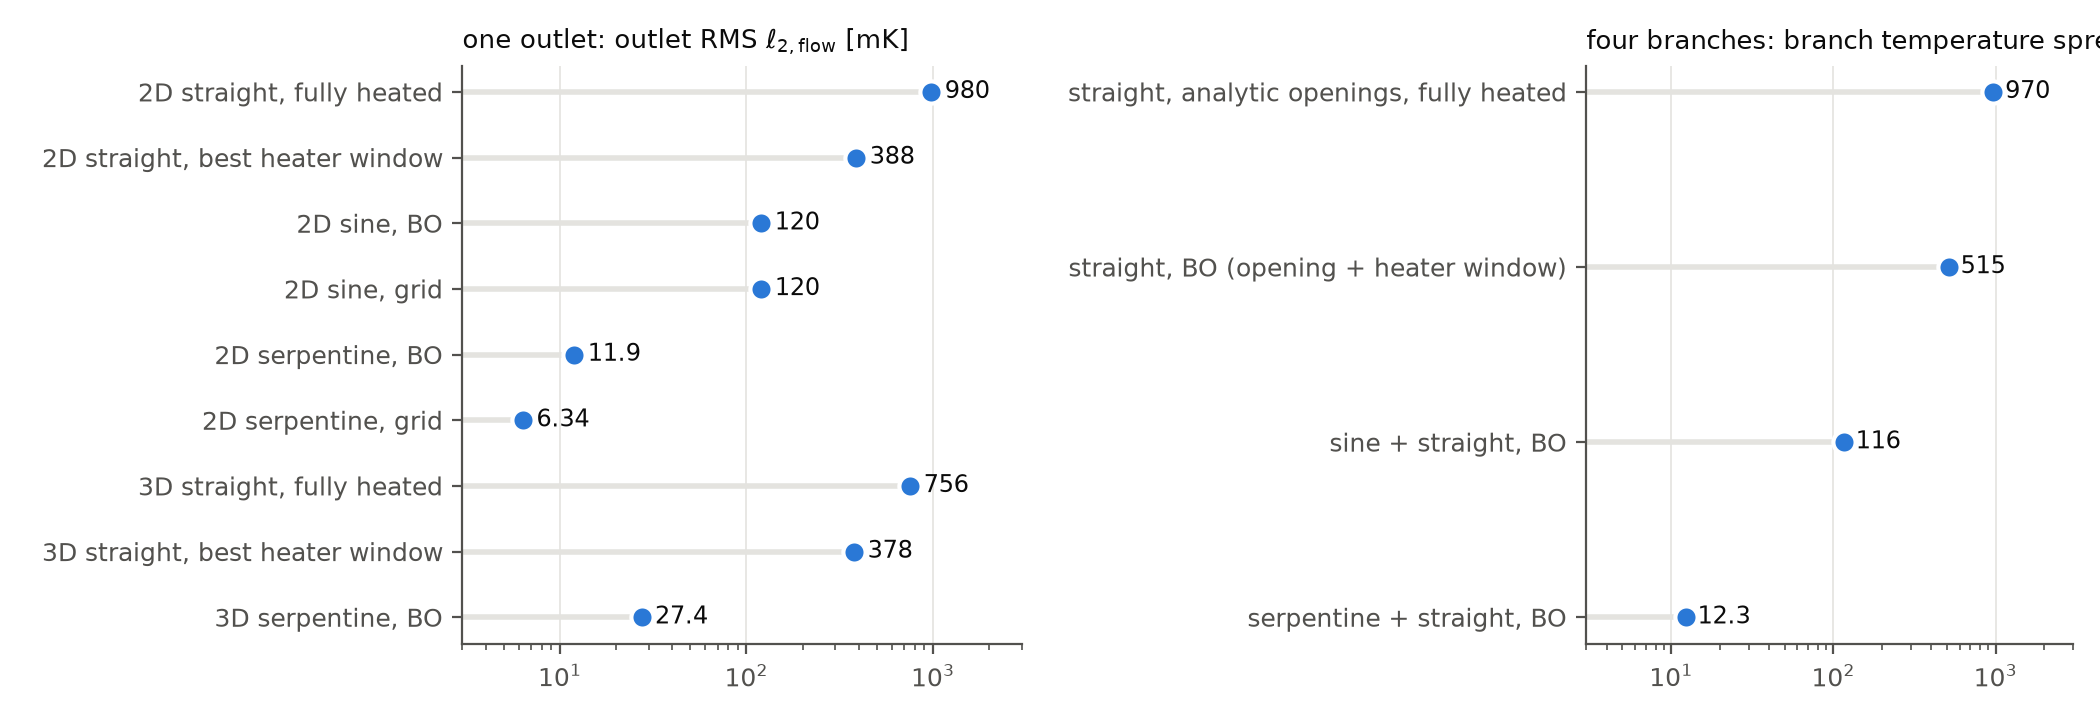
\includegraphics[width=\textwidth]{summary.png}
\caption{Best result of every run (fine mesh, log scale; lower is better). Left: RMS
deviation of the outlet temperature from the target, weighted by the flow. Right: RMS
deviation of the four branch bulk temperatures from the target. The flow imbalance of the
branched designs is in Table~\ref{tab:branch}.}
\end{figure}

\begin{table}[H]
\centering\small
\begin{tabularx}{\textwidth}{@{}l l l L@{}}
\toprule
case & method & result (fine mesh) & best design \\
\midrule
\multicolumn{4}{@{}l}{\textbf{One outlet, 2D} \quad score \ltf} \\
straight, fully heated & reference & 980\mK & heater along all 24\mm \\
straight, heater window & sweep of 209 windows & 388\mK & start 0, length 2.4\mm{} (shortest below 99\,$^\circ$C) \\
sine & BO, 50 + 3 runs & 120\mK & $\lambda$ 11.1, $a$ 1 ($A$ 2.0\mm), heater 7.2\mm \\
sine & grid, 112 + 3 runs & 120\mK & same design \\
serpentine & BO, 50 + 3 runs & 11.9\mK & $\lambda$ 8.7, $A$ 3.1, heater 14.4\mm \\
serpentine & grid, 106 + 3 runs & \textbf{6.3\mK} & $\lambda$ 8.3, $A$ 2.1, heater 9.6\mm \\
\midrule
\multicolumn{4}{@{}l}{\textbf{One outlet, 3D (depth 3\mm)} \quad score \ltf} \\
straight, fully heated & reference & 756\mK & heater on all four walls, 24\mm \\
straight, heater window & sweep of 105 windows & 378\mK & start 0, length 1.2\mm{} (shortest in the sweep) \\
serpentine & BO, 28 + 4 runs & \textbf{27.4\mK} & $\lambda$ 7.3, $A$ 3.5 (both at a bound), heater 19.2\mm \\
\midrule
\multicolumn{4}{@{}l}{\textbf{Four branches, 2D} \quad branch temperature spread / flow imbalance} \\
straight, analytic openings & reference & 970\mK{} / 0.87\,\% & $\rho$ 0.532, fully heated \\
straight & BO, 16 + 2 runs & 515\mK{} / 0.16\,\% & $\rho$ 0.540, heater 2.4\mm{} at 99\,$^\circ$C \\
sine + straight & BO, 150 + 3 runs & 116\mK{} / 0.82\,\% & $\lambda$ 10.0, $a$ 1, sine 68\,\%, heater 1 40\,\% \\
serpentine + straight & BO, 150 + 3 runs & \textbf{12.3\mK} / 3.9\,\% & $\lambda$ 7.9, $A$ 3.5, serpentine 78\,\%, no heater 2 \\
\bottomrule
\end{tabularx}
\caption{All results. ``Heater'' lengths are measured from the start of the wavy section.}
\label{tab:summary}
\end{table}

\textbf{Main findings.}
\begin{itemize}
  \item \textbf{The serpentine wins everywhere, by a factor of 10--20 over the sine and 15--150 over
        the straight channel.} At 6\,mL/min the water spends about 2\,s in the channel, and heat diffuses
        only about 0.6\mm{} in that time, against a 1.5\mm{} half-width. Only folding the flow helps.
        The serpentine can fold it much more strongly than the constant-width sine, whose amplitude is
        capped by the bend radius ($A \le 2.0\mm$ at $\lambda = 11$).
  \item \textbf{The best layout is always a short-to-medium heater at the inlet, then unheated meanders.}
        The meanders after the heater mix the hot wall layers into the core. In every wavy design the
        heater stops well before the end, at 30--80\,\% of the wavy length.
  \item \textbf{3D is 2--4$\times$ worse than 2D for the serpentine} (27\mK{} vs 6--12\mK), and its
        best design sits at the edge of the search box: the smallest wavelength and the largest amplitude
        allowed. A tighter or taller serpentine is likely to be better still.
  \item \textbf{Branched:} the serpentine + straight design brings the four branch temperatures within
        30\mK{} of each other (from 1.94\K{} for the straight reference), but at a 3.9\,\% flow imbalance,
        against 0.2--0.9\,\% for the straight and sine designs. The flow weight in the loss decides that trade-off.
  \item \textbf{BO and grid agree for the sine}, and for the serpentine the grid found a 2$\times$ better
        design. Most of that gap is coarse-mesh noise, because the coarse and fine meshes rank these
        designs differently (Section~\ref{sec:u2d}).
\end{itemize}

%=====================================================================
\section{Set-up}
%=====================================================================
\subsection{Physics (all runs)}
\begin{itemize}
  \item \textbf{Fluid.} Water with constant properties (the values used in all earlier runs) ($\rho = 972.4$\,kg/m$^3$,
        $\mu = 0.355$\,mPa\,s, $k = 0.669$\,W/mK, $c_p = 4196$\,J/kgK). Steady laminar flow at
        6\,mL/min, mean speed 11\,mm/s in the $3\times3\mm$ section, $Re \approx 91$. Fully
        developed inlet. Flow is solved first, then heat.
  \item \textbf{Temperatures.} $T_\mathrm{in} = 343.15\K$ (70\,$^\circ$C), target
        $\Tneed = T_\mathrm{in} + 2\K$, ambient 293.15\K.
  \item \textbf{Heater.} The heated walls are held at one temperature $T_\mathrm{heat}$, coupled
        through $h_\mathrm{heat} = 10^5$\,W/m$^2$K. $T_\mathrm{heat}$ is solved so that the outlet
        bulk temperature is exactly $\Tneed$, and it is limited to 99\,$^\circ$C. A design that would
        need more is \emph{clamped} and misses the target, which the loss then penalizes.
  \item \textbf{Losses.} Unheated walls lose heat with $h_\mathrm{loss} = 2$\,W/m$^2$K. The 2D
        models add the same loss for the top and bottom walls as a volume term. The four branches
        use $h_\mathrm{loss,br} = 10$\,W/m$^2$K, to stand in for longer real branches.
  \item \textbf{2D vs 3D.} The 2D models represent the channel in the $x$--$y$ plane; depth enters
        only through the flow rate and the top/bottom loss. In 2D the heater covers the two side
        walls. In 3D it covers all four walls, and a symmetry plane at mid-depth halves the model.
\end{itemize}

\subsection{Geometries}
\begin{description}
  \item[One outlet (2D).] 2\mm{} inlet port, then the 24\mm{} straight, sine or serpentine section,
        then a 3\mm{} straight before the exit line where the score is measured, then an
        adiabatic 3\mm{} extension so the outflow condition does not distort the profile.
  \item[One outlet (3D).] As in 2D: 2\mm{} inlet port, 24\mm{} channel, 3\mm{} outlet straight.
        The heater starts at $x = 2\mm$, the start of the channel.
  \item[Four branches (2D).] 2\mm{} port, then a wavy section (fraction $f$ of $L_\mathrm{main} = 24\mm$)
        with heater 1, then a straight section with heater 2, then a 6\mm{} fan into four
        branches with 2\mm{} outlet ports at 4\mm{} pitch. Both heaters start at the start of their
        section. The branch inlet widths are symmetric, $r = (1, \rho, \rho, 1)$, so a single
        opening ratio $\rho$ remains free.
  \item[Sine walls.] Centre line $A\sin(2\pi x/\lambda)$, walls offset by $w/2$ along the normal,
        so the width across the flow is 3\mm{} everywhere. The walls fold over unless
        $A \le A_\mathrm{max}(\lambda) = \min\!\big(3.5,\ \lambda^2/(4\pi^2(w/2 + 0.05))\big)$.
        The search variable is $a = A/A_\mathrm{max}(\lambda) \in [0,1]$, so every point is feasible.
  \item[Serpentine walls.] Straight legs joined by circular arcs with centre-line radius
        $R_\mathrm{bend} = 1.55\mm$, width 3\mm{} everywhere, $A \le 3.5\mm$,
        $\lambda \ge 6.5\mm$ (the arcs need $\lambda > 4R_\mathrm{bend}$). The wave ends at the apex of its last crest.
\end{description}

\subsection{Flow rate: 6 instead of 20\,mL/min}
The study plan asked for 20\,mL/min or whichever flow rate was faster to simulate. Solve
times on the same meshes:

\begin{table}[H]
\centering\small
\begin{tabular}{@{}lccc@{}}
\toprule
case & 6\,mL/min & 20\,mL/min & slow-down at 20 \\
\midrule
2D straight, coarse & 11\,s & 12\,s & 1.1$\times$ \\
2D sine, coarse / fine & 13 / 25\,s & 18 / 56\,s & 1.4--2.2$\times$ \\
2D serpentine, coarse / fine & 20 / 51\,s & 46 / 69\,s & 1.4--2.3$\times$ \\
2D branched, coarse & 19\,s & 25\,s & 1.3$\times$ \\
3D straight, coarse & 40\,s & 46\,s & 1.2$\times$ \\
3D sine, coarse & 62\,s & 529\,s & 8.5$\times$ (only solved with a flow ramp) \\
\bottomrule
\end{tabular}
\end{table}

6\,mL/min is faster, converges reliably in 3D, and avoids the separated and possibly unsteady
flow that a steady 2D model cannot represent at 20\,mL/min. The geometry still matters at
6\,mL/min: the residence time is about 2.2\,s, and the thermal diffusion length
$\sqrt{\alpha t} \approx 0.6\mm$ is well short of the 1.5\mm{} half-width. In single test
runs the straight, sine and serpentine shapes differed by 12--16$\times$, so the flow was
not raised to 10\,mL/min.

\subsection{Meshes}
\begin{itemize}
  \item \textbf{2D:} mapped quadrilateral meshes graded towards the walls; the fine mesh has half the
        element size of the coarse one. Fine meshes: 45--75k elements (one outlet), 105--165k (branched).
  \item \textbf{3D:} mapped prisms. Coarse: 20 across the width, $h_{xy}$ 0.12\mm, 8 layers in half
        the depth (75k elements). Fine: 28 across, $h_{xy}$ 0.08\mm, 12 layers (235--285k).
        Mesh check in Section~\ref{sec:u3d}.
\end{itemize}

%=====================================================================
\section{Methods}
%=====================================================================
\subsection{Losses}
All scores are computed in Python from the raw outlet data that each run stores:
\begin{align*}
  \ltf &= \sqrt{\int u\,(T-\Tneed)^2\,dA \Big/ \int u\,dA}, \qquad
  \ell_{2,\mathrm{area}} = \sqrt{\tfrac{1}{A}\int (T-\Tneed)^2\,dA},\\
  \text{branch} &= \underbrace{\frac{\mathrm{RMS}_i(T_{b,i}-\Tneed)}{\Delta T}}_{\text{branch\_T}/\Delta T}
                 + 0.25\,\underbrace{\mathrm{RMS}_i\!\left(\frac{Q_i}{\bar Q}-1\right)}_{\text{branch\_Q}} .
\end{align*}
\begin{itemize}
  \item The one-outlet runs minimize $\ltf$, the RMS deviation seen by the fluid that actually
        leaves. It is never smaller than $|T_\mathrm{bulk} - \Tneed|$, so an under-heated outlet
        cannot score well. ($\ell_{2,\mathrm{area}}$ can be fooled by slow, hot fluid near the walls.)
  \item The branched runs minimize ``branch''. $T_{b,i}$ and $Q_i$ are the bulk temperature and
        flow rate of branch $i$. With the flow weight 0.25, a 1\,\% flow imbalance costs as much as
        5\mK{} of temperature spread.
  \item The field-map titles show $\ell_{2,\mathrm{area}}$. The tables use the loss that was optimized.
\end{itemize}

\subsection{Heater sweeps on one flow solve}
The flow, and therefore the mesh, does not depend on where the heater is. Each geometry
therefore gets one flow solve, followed by heat-only re-solves for a list of heater windows, and
is scored by its best window:
\begin{itemize}
  \item 2D wavy designs: heater 1 from the start of the wavy section, length 10, 20, \dots, 100\,\%.
  \item 2D straight references (one outlet and branched): every start 0--90\,\% in 5\,\% steps
        and every length from 5\,\% in 5\,\% steps with start + length $\le 100\,\%$, 209 windows.
  \item 3D straight reference: the same starts, every second length (5, 15, 25, \dots\,\%), 105 windows.
  \item 3D serpentine: from the channel start, length 2.4--24\mm{} in 10 steps.
\end{itemize}
The heater length is therefore not a BO or grid variable. The one-outlet searches have only two
variables, ($\lambda$, $a$) or ($\lambda$, $A$).

\subsection{Bayesian optimization (BO)}
\begin{enumerate}
  \item Variables are mapped to $[0,1]$ ($\lambda$ on a log scale). Constraints are checked before
        a run, so infeasible designs cost nothing.
  \item \textbf{Initial design:} $n_\mathrm{init}$ space-filling runs on the coarse mesh (Latin
        hypercube, then a greedy maximin selection).
  \item \textbf{Surrogate:} a Gaussian process on $\log_{10}(\text{loss})$, with a Mat\'ern-5/2
        kernel, one length scale per variable, and a white-noise term that absorbs mesh noise.
  \item \textbf{Next points:} maximize expected improvement over 20k random and local candidates.
        Parallel workers get batches through the constant-liar trick.
  \item \textbf{Failed runs} (bad geometry or no convergence) are recorded and penalized at the
        worst observed value + 0.5 decades.
  \item \textbf{Fine stage:} the best $k$ distinct coarse designs are re-run on the fine mesh. The
        reported result is the best fine run.
\end{enumerate}

\subsection{Staged grid search}
The grid works in the same unit cube, so log-scaled variables are spaced logarithmically
(\texttt{comsol\_opt/gridcase.py}). It reads a \texttt{grid:} section from the same YAML file
as BO. It shares BO's workers, history file, resume and losses.
\begin{itemize}
  \item \textbf{Level 0:} a full grid (sine: 12 $\lambda$ $\times$ 8 $a$; serpentine: 10 $\lambda$ $\times$ 8 $A$).
  \item \textbf{Zoom 1:} $3\times3$ points at $\pm\tfrac12$ step around the 3 best distinct designs.
  \item \textbf{Zoom 2:} $3\times3$ points at $\pm\tfrac14$ step around the best design.
  \item \textbf{Fine stage:} the 3 best on the fine mesh.
\end{itemize}

\subsection{Which runs got a grid}
With the heater handled by the sweep, the one-outlet searches have only two variables, so BO
(50 runs) and a grid (about 110 runs) cost about the same, and both were run for the 2D cases.
\begin{itemize}
  \item The 3D grid was dropped: same variables as the 3D BO, and about 4$\times$ the cost.
  \item The branched grid was dropped as agreed: five variables, and about 6--7\,h for little gain over BO.
\end{itemize}

\subsection{Run time}
All runs ran on the shared server (i7-14700F), 3--4 COMSOL servers side by side, each with 4 cores.

\begin{table}[H]
\centering\small
\begin{tabular}{@{}llr@{}}
\toprule
stage & runs & wall time \\
\midrule
A & 2D references, branched straight BO & 48\,min \\
B & 2D one-outlet BO (sine, serpentine) & 14\,min \\
C & 2D one-outlet grids & 24\,min \\
D & branched BO (sine, serpentine) & 53\,min \\
E & 3D straight reference, 3D mesh check & 25\,min \\
F & 3D serpentine BO (+ 2 extra fine checks) & 32 + 10\,min \\
\midrule
 & total (01:32--04:56) & 3\,h 24\,min \\
\bottomrule
\end{tabular}
\end{table}

%=====================================================================
\section{One outlet, 2D}\label{sec:u2d}
%=====================================================================
\begin{figure}[H]
\centering
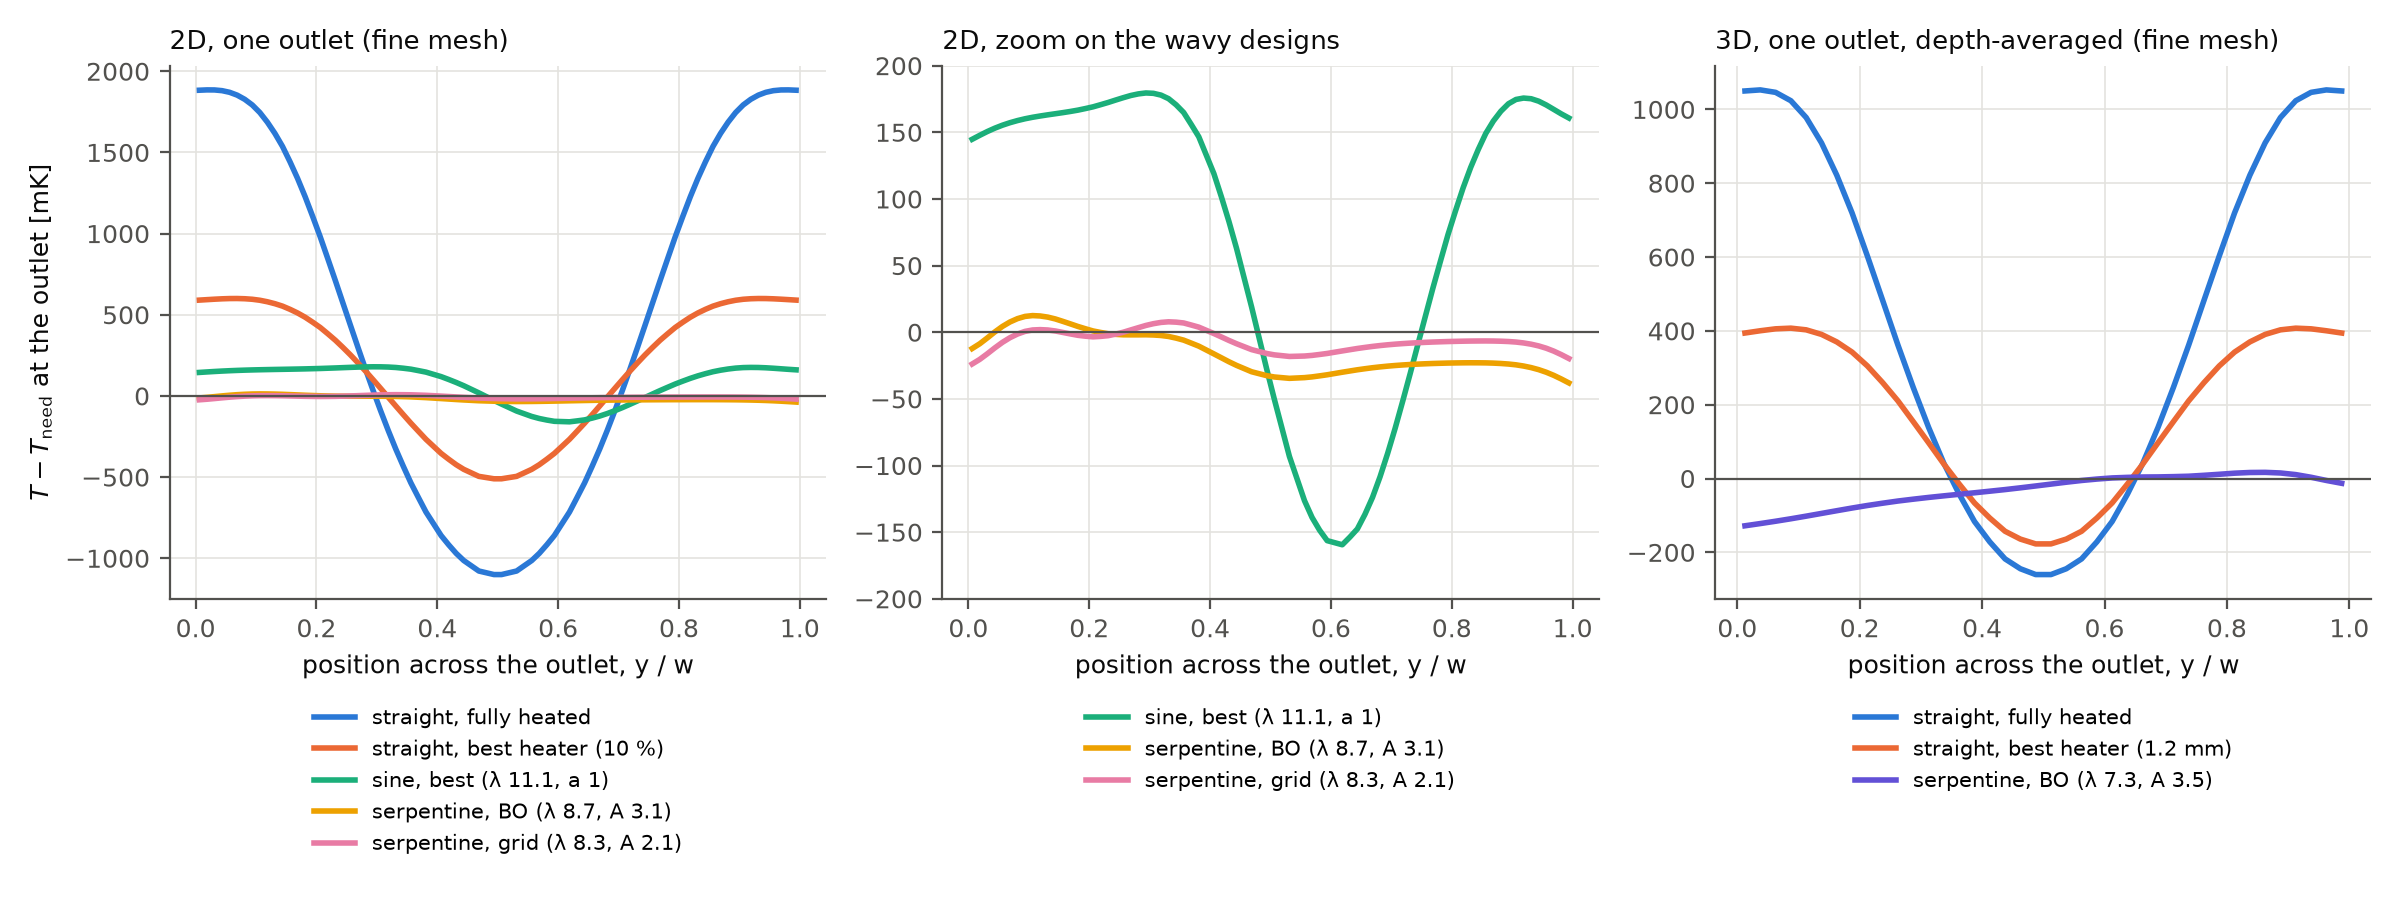
\includegraphics[width=\textwidth]{outlet_profiles.png}
\caption{Outlet temperature profiles of the best designs. The straight channel leaves hot
fluid at the walls and cold fluid in the core. A short inlet heater halves the error, because
the rest of the channel then has time to even it out. The serpentine profiles are flat to within
$\pm 40\mK$. In 3D the serpentine leaves a slight tilt across the outlet.}
\end{figure}

\begin{figure}[H]
\centering
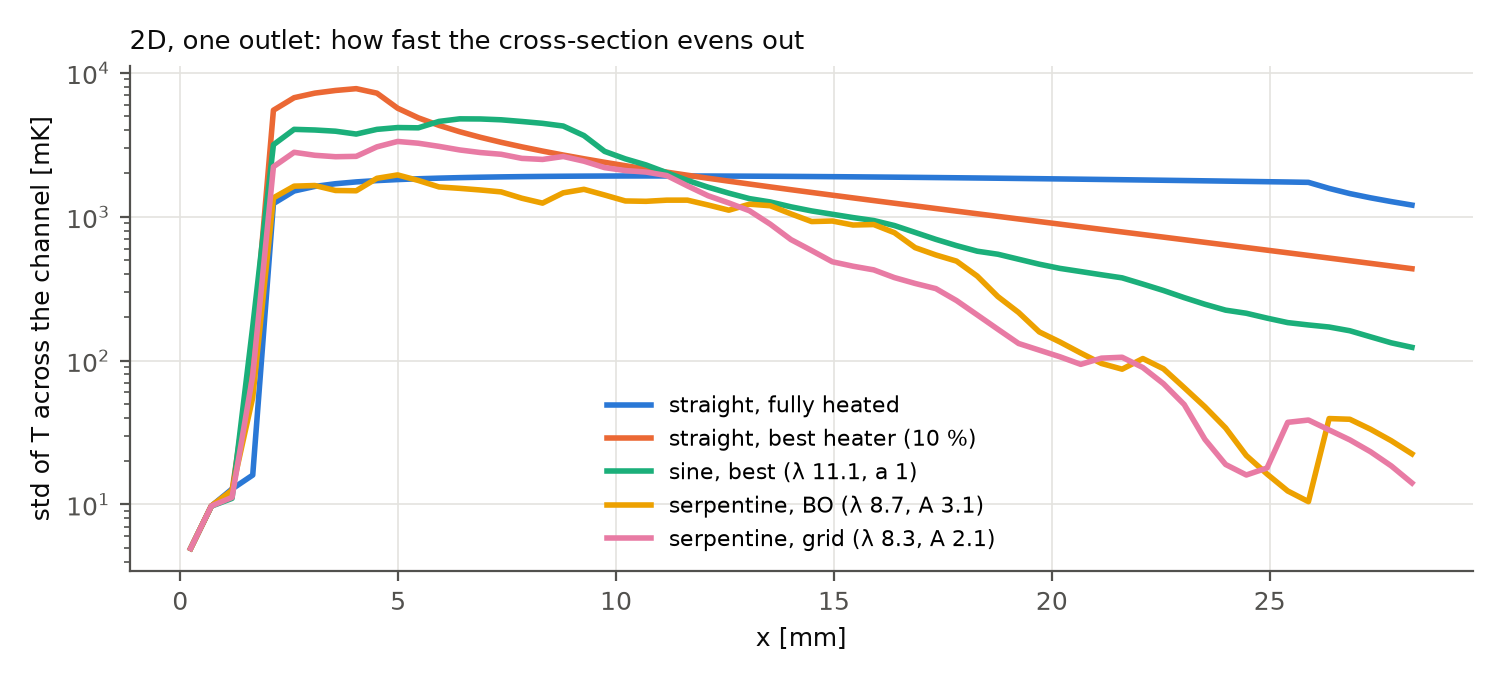
\includegraphics[width=0.8\textwidth]{along_x_2d.png}
\caption{Spread of the temperature across the channel along $x$ (2D). The heater starts at
$x = 2\mm$. The straight channel evens out only by diffusion, slowly. The serpentines lose a
decade every 6--8\mm{} once the heater stops.}
\end{figure}

\subsection{Straight references}
\begin{itemize}
  \item \textbf{Fully heated:} 980\mK. The heater only has to reach 76\,$^\circ$C, but the
        wall layers stay hot (+1.9\K) and the core stays cold ($-1.1\K$).
  \item \textbf{Best heater window:} 388\mK, a 2.4\mm{} heater right at the inlet at
        98\,$^\circ$C, just under the limit.
  \item \textbf{The best window is the shortest one that reaches the target} (start 0, 2.4\mm).
        The answer is simply ``heat early, then let it diffuse''. The 1.2\mm{} windows would need
        more than 99\,$^\circ$C.
\end{itemize}

\subsection{Sine (constant width)}
\begin{itemize}
  \item \textbf{BO and grid find the same optimum:} $\lambda \approx 11.1\mm$ and $a = 1$ (on the
        bend limit, $A = 2.0\mm$), heater 30\,\%, 120\mK.
  \item \textbf{Every good design is on the bend limit} ($a = 1$, Figure~\ref{fig:land}). This is the same
        result as the earlier 1\mm{} work. The constant-width sine cannot bend sharply enough
        to fold a 3\mm{} channel.
  \item \textbf{3.2$\times$ better than the best straight channel}, but still 10--20$\times$ worse than the serpentine.
\end{itemize}

\subsection{Serpentine}
\begin{itemize}
  \item \textbf{BO: 11.9\mK} ($\lambda$ 8.7, $A$ 3.1, heater 60\,\%).
  \item \textbf{Grid: 6.3\mK} ($\lambda$ 8.3, $A$ 2.1, heater 40\,\%).
  \item \textbf{Same valley.} Both lie in a narrow valley at $\lambda \approx 8.3$--$8.7\mm$ that
        runs from $A \approx 1.9$ to 3.5 (Figure~\ref{fig:land}). Outside it the score is 10$\times$ worse.
  \item \textbf{The 2$\times$ gap is mostly mesh noise.} The coarse and fine meshes disagree by up to
        1.7$\times$ here:
  \begin{itemize}
    \item BO's coarse best (\#35, $A$ 2.16) scored 12.3\mK{} coarse but 20.6\mK{} fine;
    \item BO's coarse second (\#31, $A$ 3.10) scored 14.0\mK{} coarse but 11.9\mK{} fine;
    \item the grid's fine re-runs of 3 neighbouring points ($A$ 1.88 / 2.0 / 2.13) gave 10.9 / 6.5 / 6.3\mK.
  \end{itemize}
  \item \textbf{Ranking within 2$\times$ needs the fine mesh.} The grid happened to fine-check the best
        spot of the valley.
\end{itemize}

\begin{figure}[H]
\centering
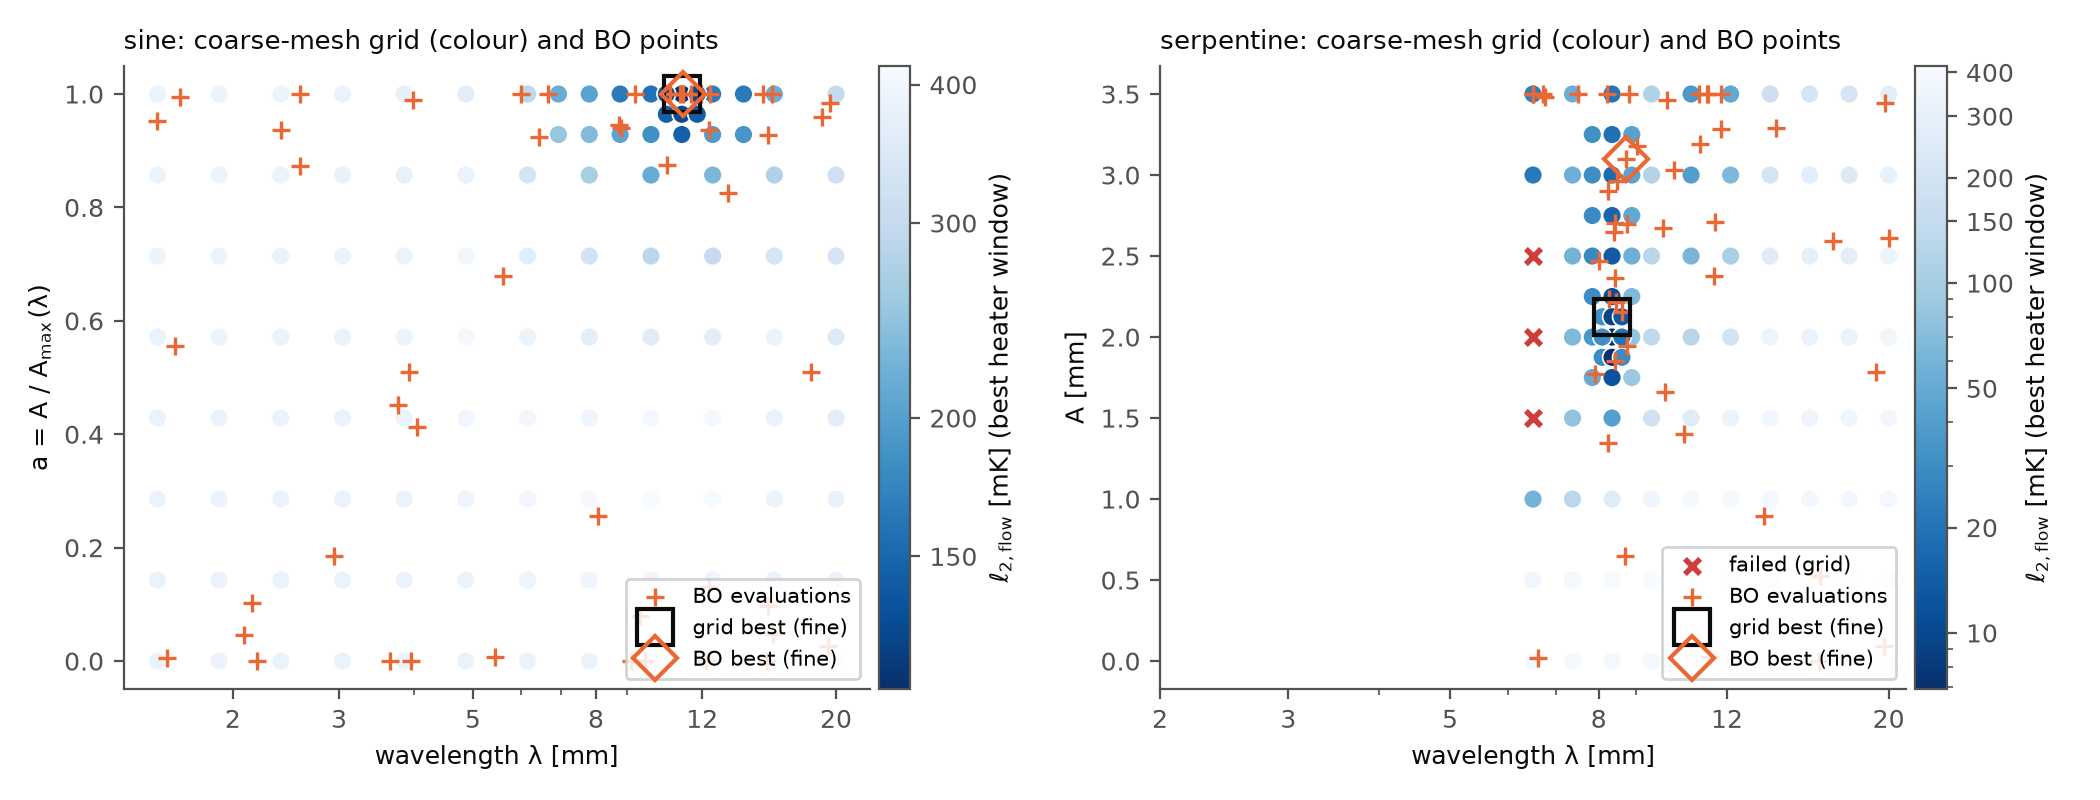
\includegraphics[width=\textwidth]{grid_landscape.png}
\caption{Coarse-mesh grid of the 2D one-outlet sine (left) and serpentine (right), with the
BO evaluations ($+$) and both fine-mesh winners. Colour: $\ltf$ with the best heater window,
dark is better. The serpentine $\lambda$ range starts at 6.5\mm.}
\label{fig:land}
\end{figure}

\begin{figure}[H]
\centering
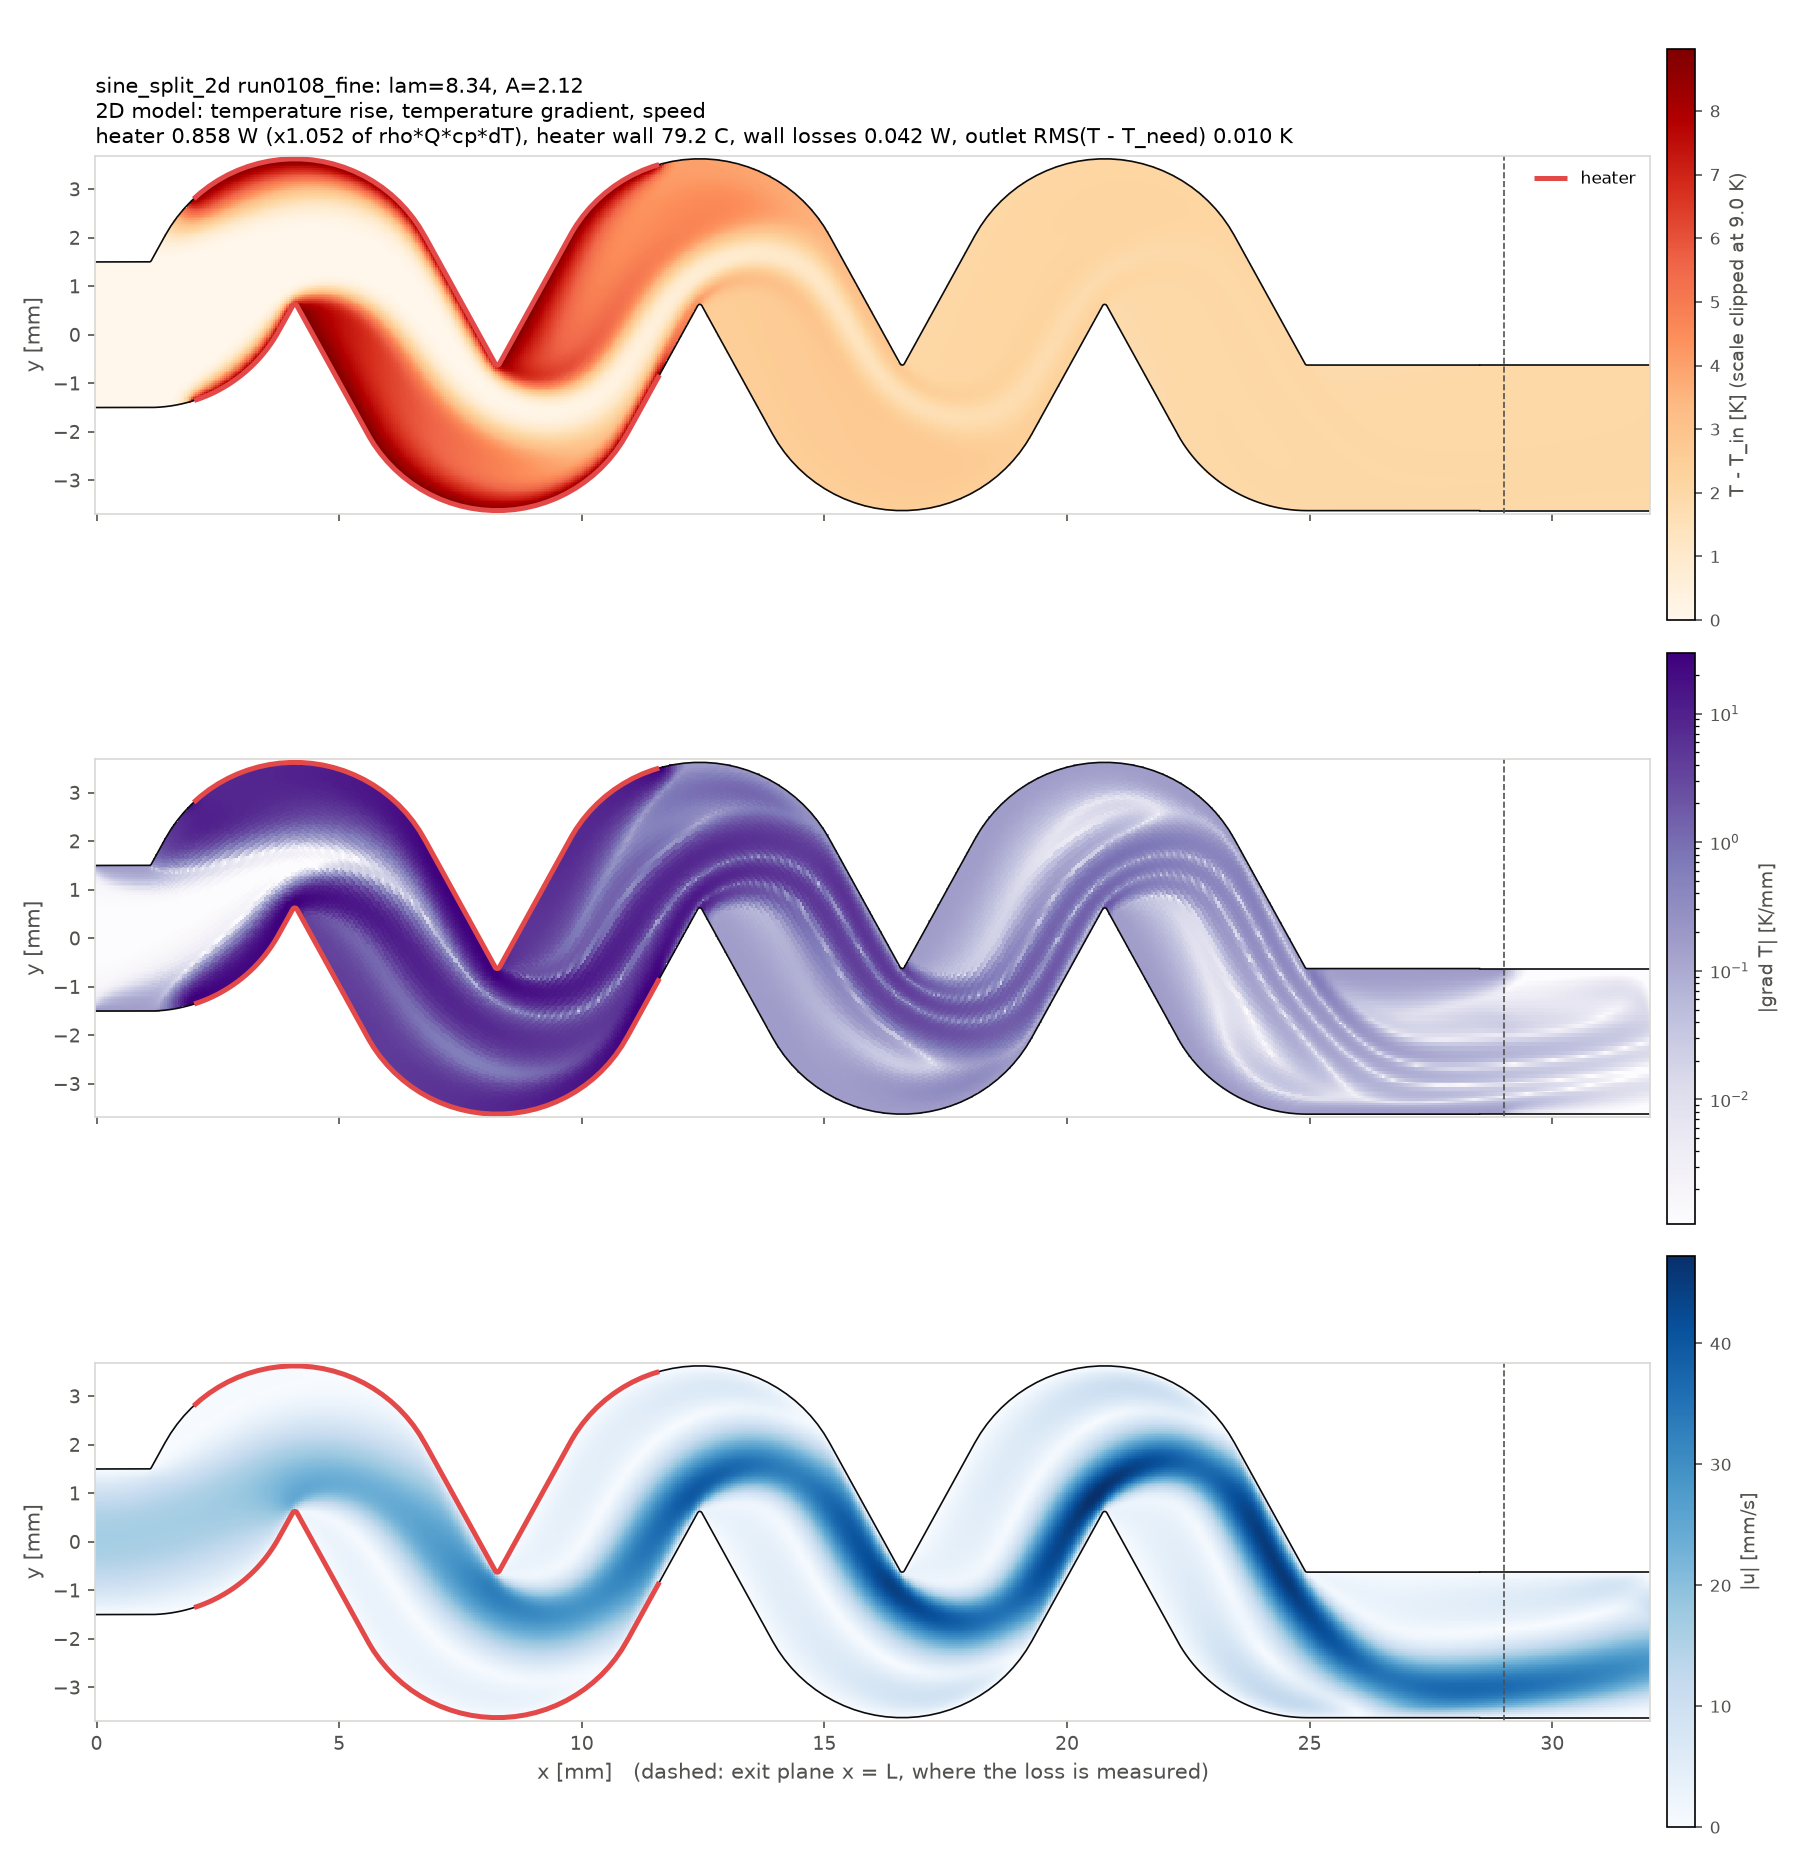
\includegraphics[width=0.85\textwidth]{runs/final_u2d_serp_grid_maps.png}
\caption{Best 2D design (serpentine, grid \#108). A 9.6\mm{} heater at 79\,$^\circ$C on the first
bends, then three unheated bends fold the hot wall layers into the core.}
\end{figure}

%=====================================================================
\section{One outlet, 3D}\label{sec:u3d}
%=====================================================================
\subsection{Mesh check}
One serpentine ($\lambda$ 8, $A$ 3) on three meshes, three heater lengths each:

\begin{table}[H]
\centering\small
\begin{tabular}{@{}lrrccc@{}}
\toprule
mesh & elements & time & heater 2.4\mm & heater 12\mm & heater 24\mm \\
\midrule
coarse (20 across, $h_{xy}$ 0.12, 8 layers) & 75k & 231\,s & 30.4\mK & 44.7\mK & 91.7\mK \\
fine (28, 0.08, 12) & 235k & 497\,s & 41.6\mK & 46.3\mK & 80.5\mK \\
reference (36, 0.06, 16) & 535k & 618\,s & 43.3\mK & 44.6\mK & 77.9\mK \\
\bottomrule
\end{tabular}
\end{table}

\begin{itemize}
  \item \textbf{The fine mesh is within 4\,\% of the reference.}
  \item \textbf{The coarse mesh reads up to 30\,\% low,} but it orders the heater lengths the same
        way. It was used for the BO search, and only fine results are reported.
\end{itemize}

\subsection{Straight references}
\begin{itemize}
  \item \textbf{Fully heated:} 756\mK. That is lower than 2D (980\mK), because in 3D the heater also
        covers the top and bottom walls.
  \item \textbf{Best window:} 378\mK, a 1.2\mm{} heater at the inlet (93\,$^\circ$C). This is the
        shortest window in the sweep, and it stays below 99\,$^\circ$C, so an even shorter one might do slightly better.
\end{itemize}

\subsection{Serpentine BO}
\begin{itemize}
  \item \textbf{Budget:} 8 initial and 20 BO runs (2 failed to converge), then the 4 best distinct
        designs on the fine mesh.
  \item \textbf{Best: \#29 at 27.4\mK} ($\lambda$ 7.26, $A$ 3.5, heater 19.2\mm, wall at 72.5\,$^\circ$C);
        \#28 ($\lambda$ 6.5, $A$ 3.43) scored 28.0\mK.
  \item \textbf{The two extra fine checks were worse:} 64.8 and 54.7\mK{} at $\lambda \approx 9.1$.
  \item \textbf{The optimum is on the edge of the box.} The best designs have the smallest $\lambda$
        and the largest $A$ allowed, so the search was stopped by its bounds, not by the physics.
  \item \textbf{3D prefers a long, cool heater.} 2D prefers a short, hot one. In 3D the bends drive
        a secondary flow over the depth, so the fluid keeps mixing while it is being heated. The cool
        wall (72.5\,$^\circ$C, only 0.5\K{} above the outlet target) leaves little to mix afterwards.
\end{itemize}

\begin{figure}[H]
\centering
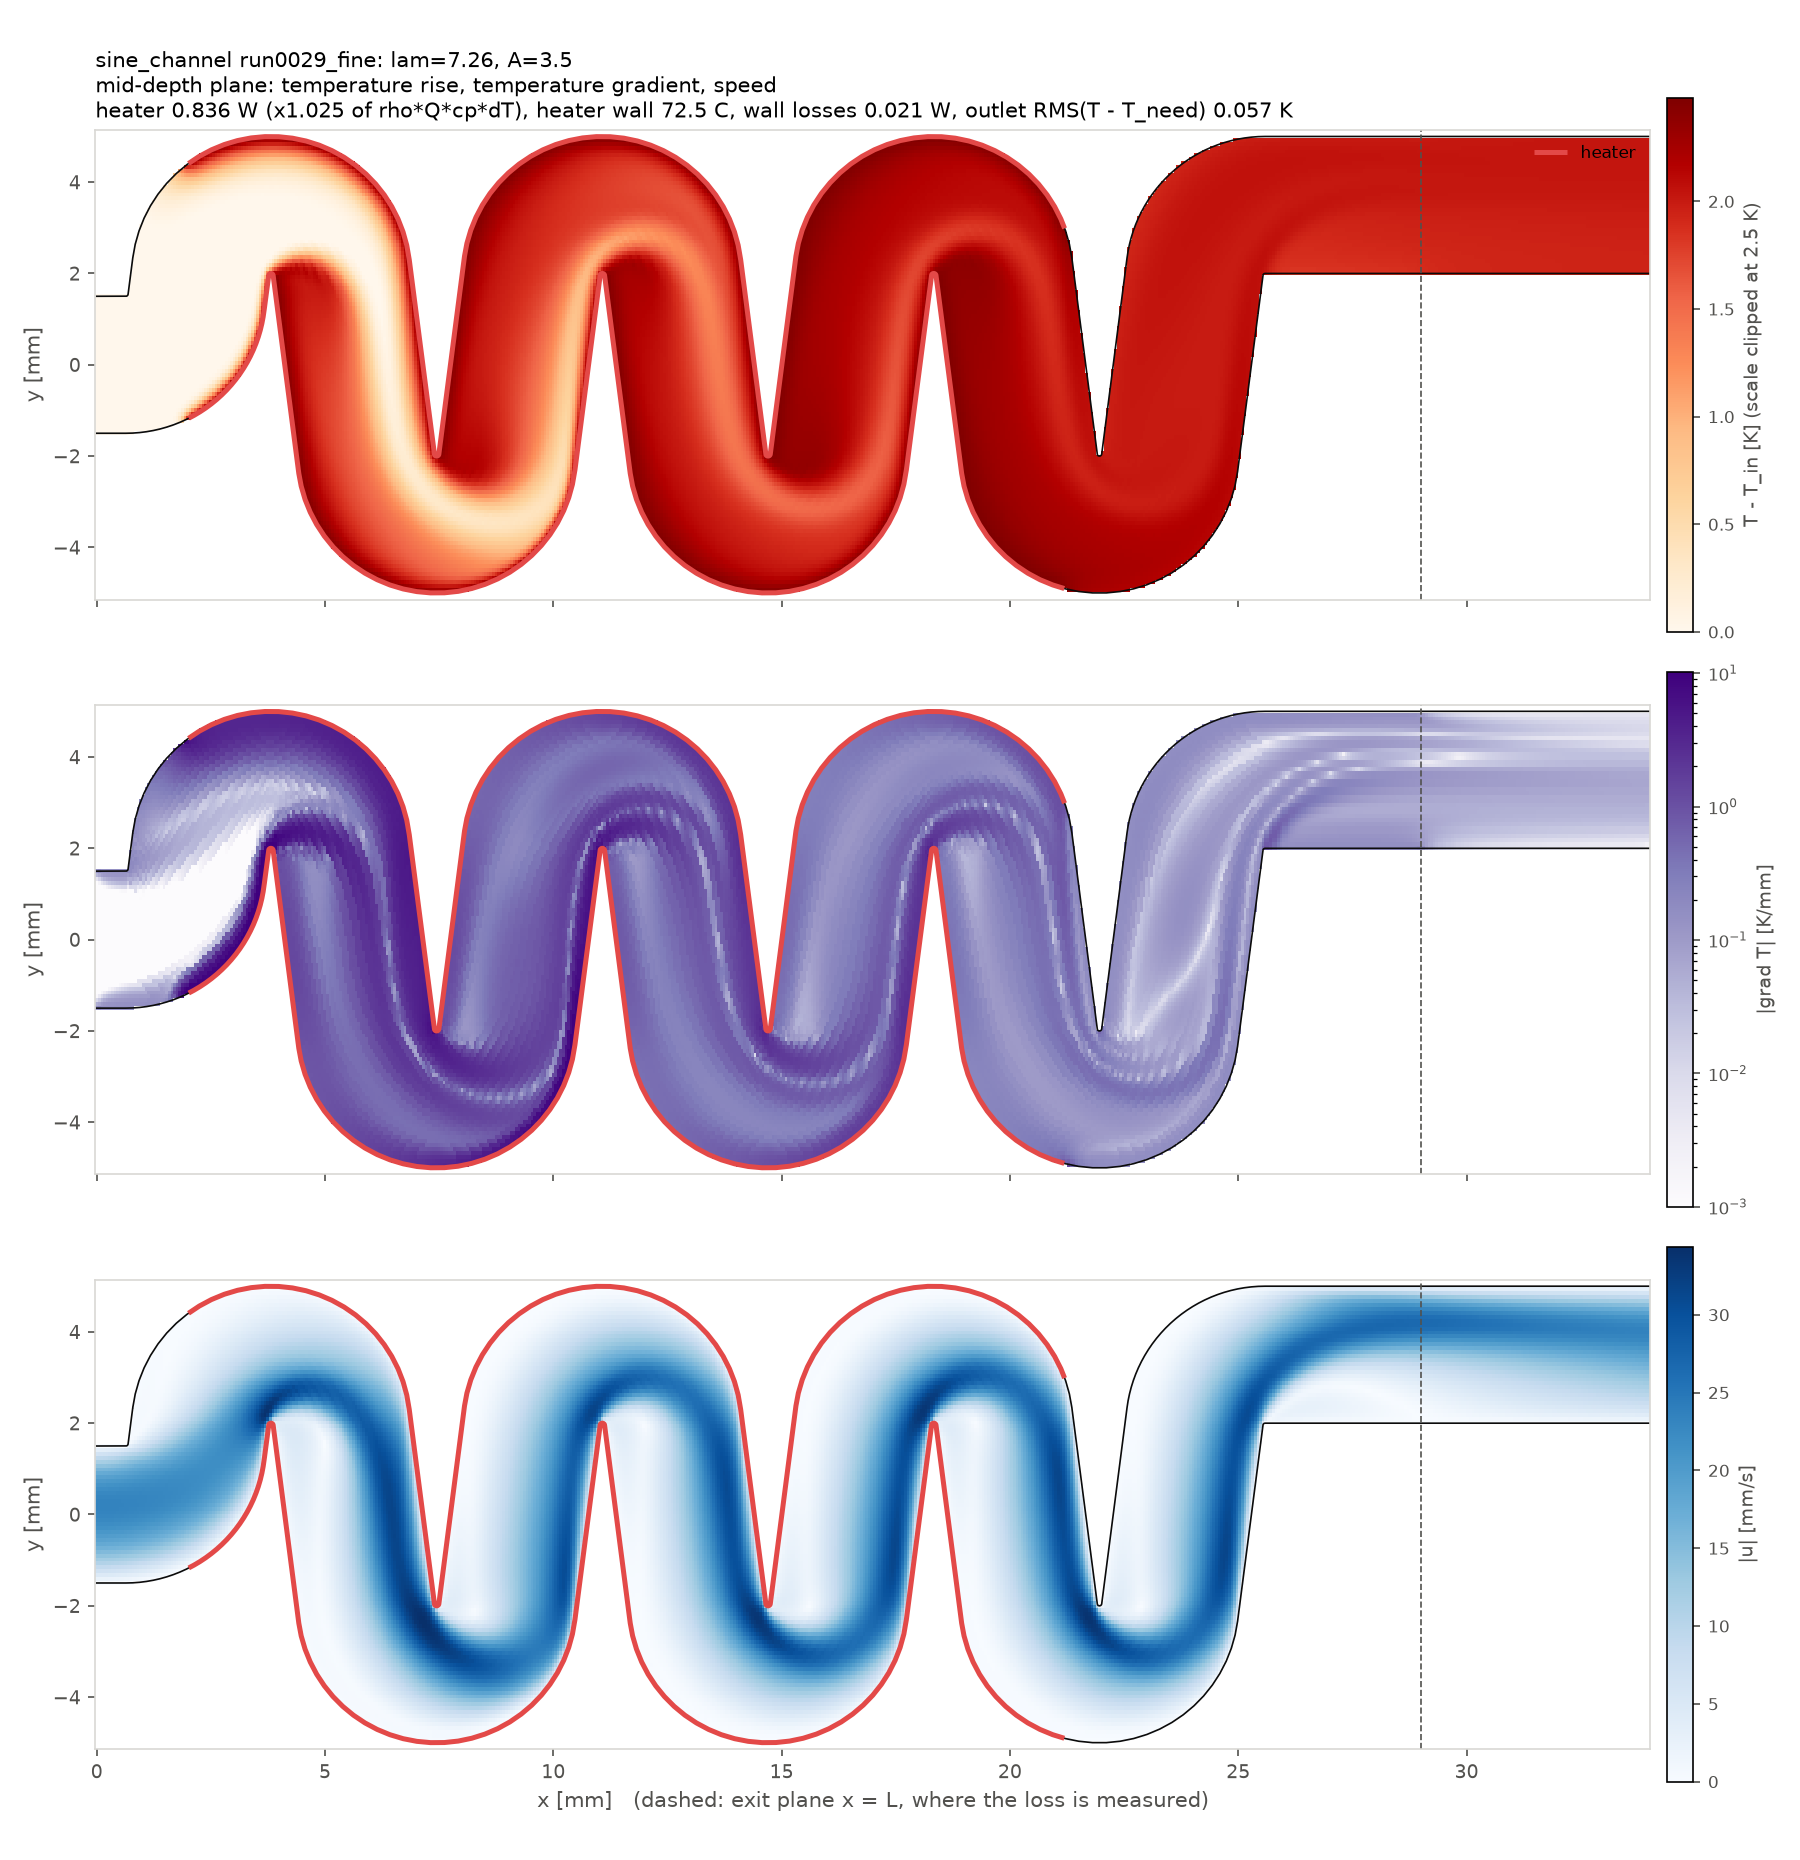
\includegraphics[width=0.85\textwidth]{runs/final_u3d_serp_maps.png}
\caption{Best 3D design (\#29), mid-depth plane. The heater covers 19.2\mm{} at 72.5\,$^\circ$C.}
\end{figure}

\textbf{2D vs 3D.}
\begin{itemize}
  \item The 3D serpentine (27\mK) is 2--4$\times$ worse than the 2D ones (6--12\mK).
  \item Its best $\lambda$ (7.3) is shorter than in 2D (8.3--8.7).
  \item The 2D results do not transfer quantitatively to a 3\mm{} deep channel, where the top and
        bottom walls matter as much as the side walls. 2D is still a good first filter for which shapes work.
\end{itemize}

%=====================================================================
\section{Four branches, 2D}\label{sec:br}
%=====================================================================
\subsection{Reference: analytic openings}
\begin{itemize}
  \item \textbf{Equal-flow cuts.} For a parabolic profile $u \propto \eta(1-\eta)$ across the channel,
        the flow through $[0,\eta]$ is $F(\eta) = 3\eta^2 - 2\eta^3$. Equal quarters need
        $F(\eta_1) = \tfrac14$, i.e.\ cuts at $\eta = 0.326,\ 0.5,\ 0.674$.
  \item \textbf{Opening ratio.} The inlet widths are then $0.326w,\ 0.174w,\ 0.174w,\ 0.326w$, so
        $\rho = 0.174/0.326 = 0.532$.
  \item \textbf{Flows:} within $\pm 0.87\,\%$, because the outer branches are longer and resist more.
  \item \textbf{Temperatures:} fully heated, the outer branches take the hot wall fluid ($+0.96\K$)
        and the inner branches the cold core ($-0.98\K$).
\end{itemize}

\subsection{Results}
\begin{table}[H]
\centering\footnotesize\setlength{\tabcolsep}{4pt}
\begin{tabular}{@{}lccccc@{}}
\toprule
design & $T_{b,i} - \Tneed$ [mK] & max$-$min & RMS & $Q_i/\bar Q - 1$ [\%] & loss \\
\midrule
straight, reference & $+962,\ -979,\ -979,\ +962$ & 1940\mK & 970\mK & $\pm 0.87$ & 0.487 \\
straight, BO & $+162,\ -711,\ -711,\ +162$ & 873\mK & 515\mK & $\pm 0.16$ & 0.258 \\
sine + straight & $+139,\ -94,\ -133,\ +90$ & 273\mK & 116\mK & $+0.2,\ +0.8,\ +0.4,\ -1.4$ & 0.060 \\
serpentine + straight & $+10,\ +10,\ +1,\ -20$ & 30\mK & 12.3\mK & $+1.4,\ -4.9,\ -2.1,\ +5.6$ & 0.016 \\
\bottomrule
\end{tabular}
\caption{Best branched designs (fine mesh), branches in order across the fan.}
\label{tab:branch}
\end{table}

\begin{itemize}
  \item \textbf{Straight, BO over $\rho$ and the heater window.}
  \begin{itemize}
    \item $\rho = 0.540$, close to the analytic 0.532, gives the best flow balance (0.16\,\%).
    \item Temperature cannot be fixed in a straight channel. The best is a 2.4\mm{} heater at the
          99\,$^\circ$C limit, and even that misses the bulk target by $-0.27\K$.
  \end{itemize}
  \item \textbf{Sine + straight.}
  \begin{itemize}
    \item Sine on 68\,\% of the length at the bend limit, heater 1 on 40\,\% of the sine, heater 2 on
          97\,\% of the straight.
    \item 116\mK, 0.8\,\%: 4.4$\times$ better than the straight channel in temperature.
    \item The fine re-run of another candidate (\#152, $\rho$ 0.81) got 29\mK{} but 20\,\% flow
          imbalance. Wider inner openings trade flow balance for temperature.
  \end{itemize}
  \item \textbf{Serpentine + straight.}
  \begin{itemize}
    \item Serpentine on 78\,\% of the length at $A = 3.5\mm$ (the bound), heater 1 on 70\,\% of it,
          no heater 2.
    \item 12.3\mK{} RMS and a 30\mK{} spread: 80$\times$ lower RMS than the reference.
    \item The flow balance is worse (3.9\,\% RMS, up to 5.6\,\%). The jet leaving the last bend
          still leans to one side when it reaches the fan. The best opening ratio is 0.47, below the
          analytic 0.53.
    \item The neighbouring designs (\#151, \#152, with heater 2 on) score almost the same: 12.8--20\mK,
          2.6--4.2\,\%.
    \item 8 of 150 runs failed (bends that do not fit).
  \end{itemize}
\end{itemize}

\begin{figure}[H]
\centering
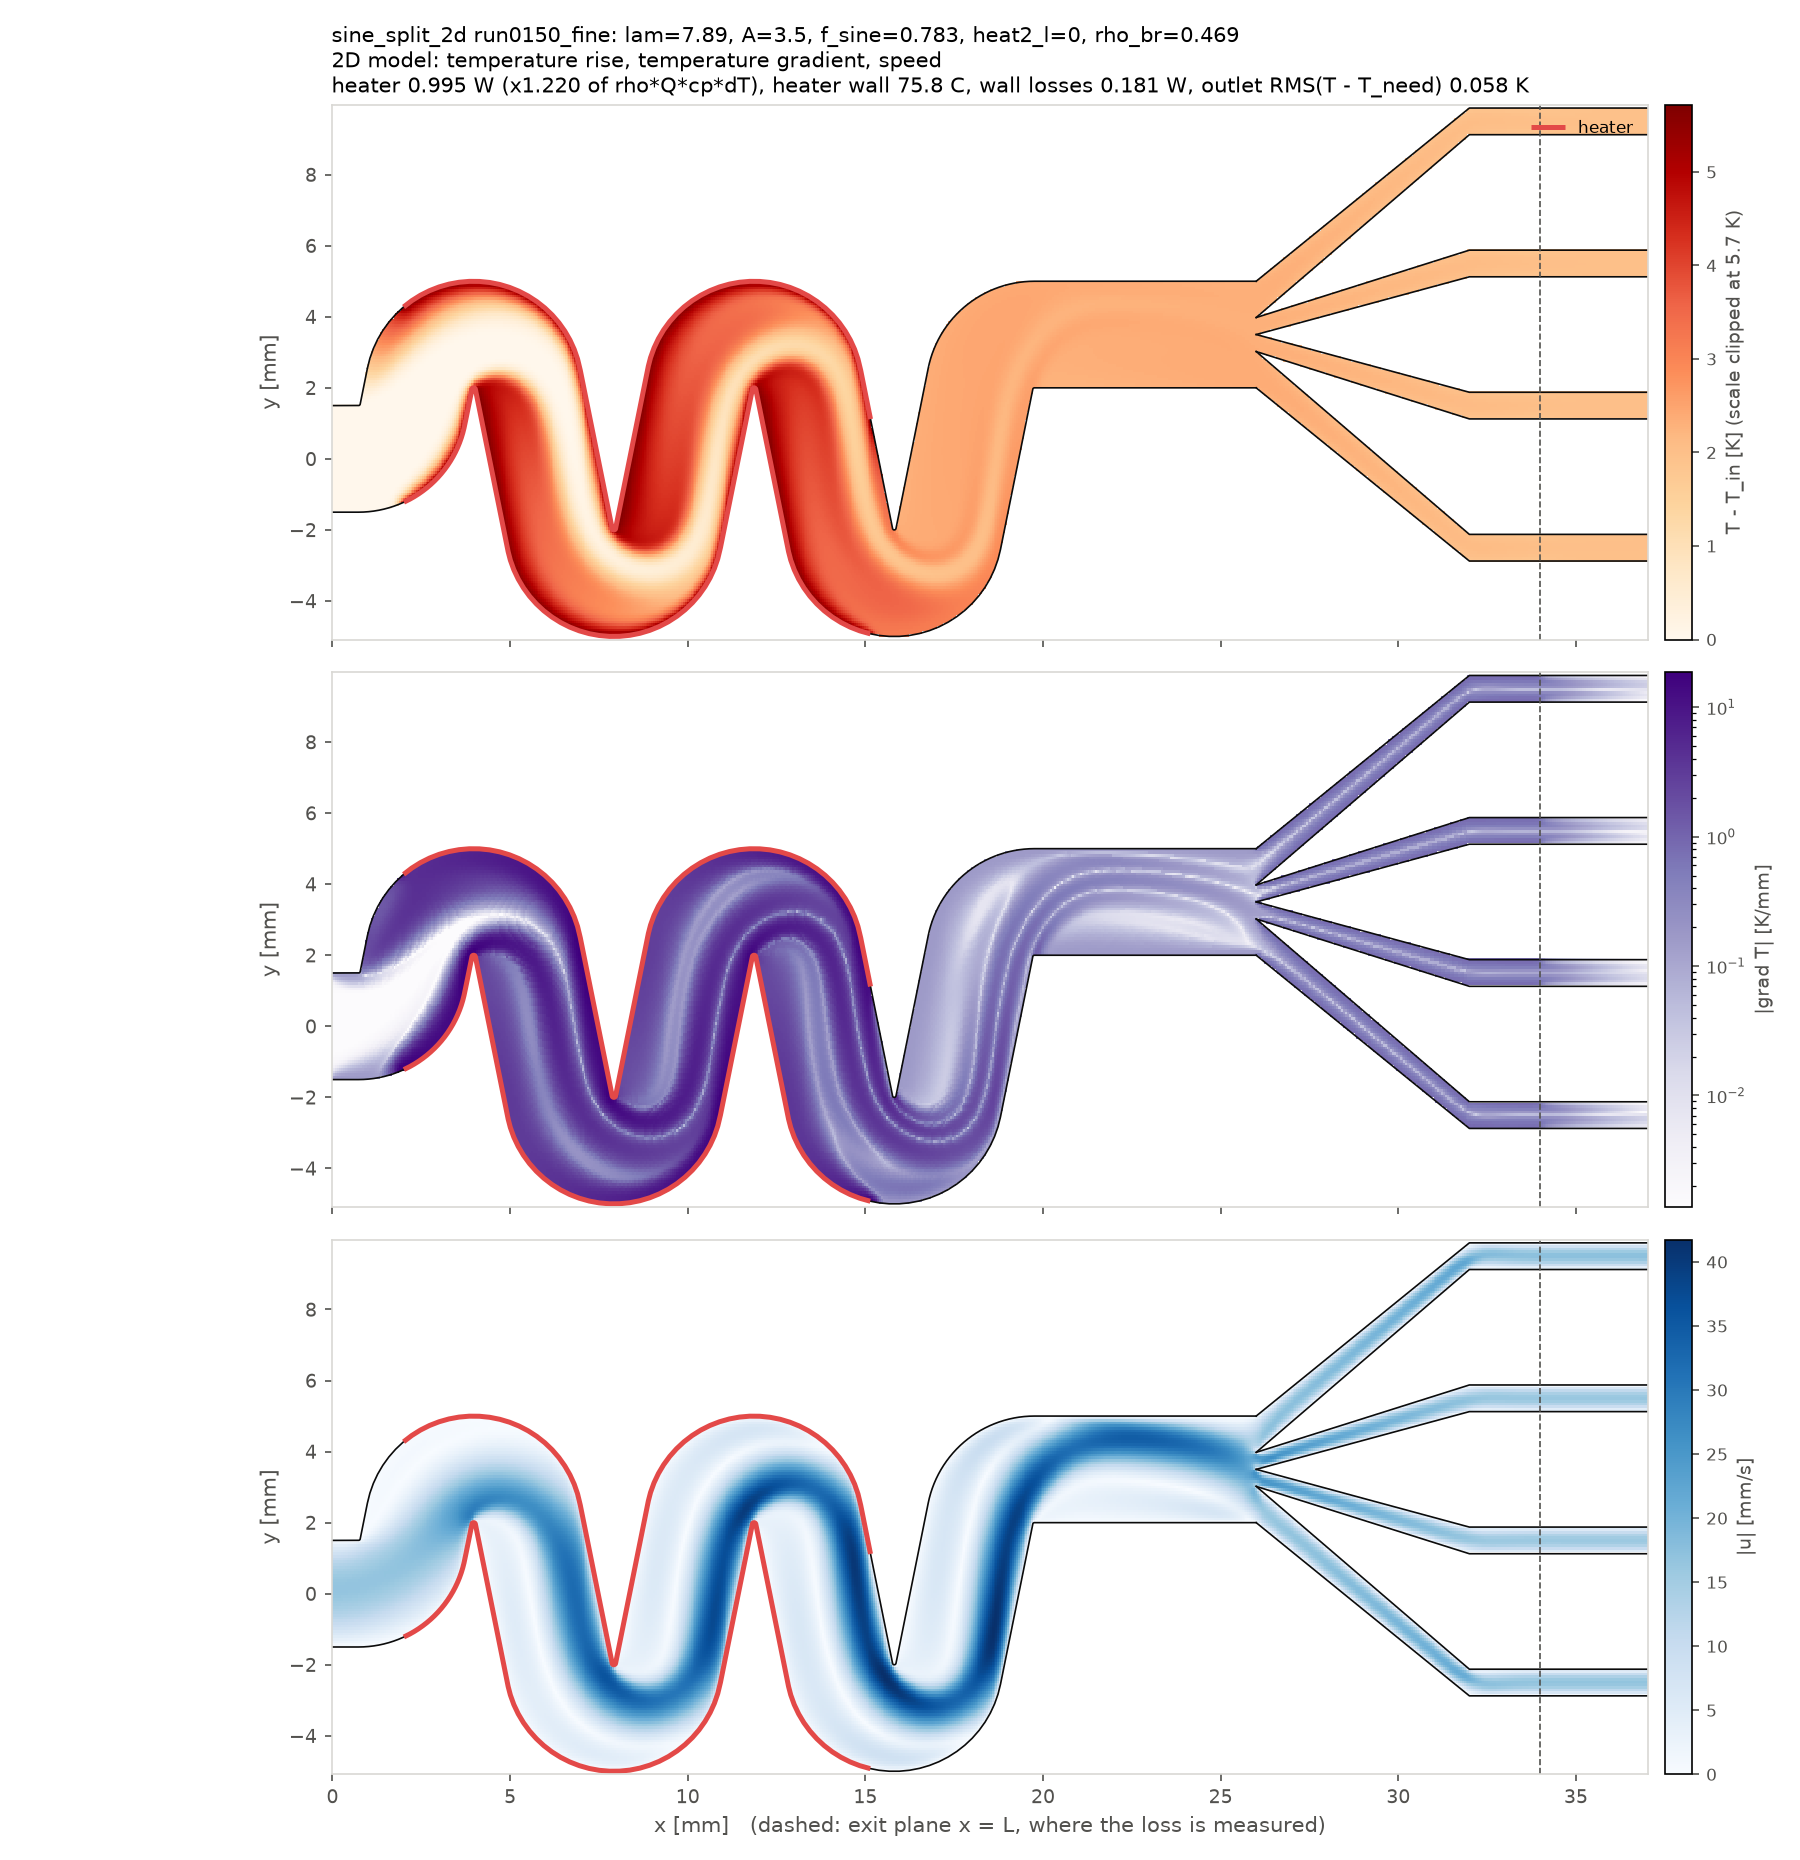
\includegraphics[width=0.85\textwidth]{runs/final_b2d_serp_maps.png}
\caption{Best branched design (serpentine + straight, \#150). Speed panel: the jet from the last
bend runs along the upper wall of the straight section and is still off-centre at the fan.}
\end{figure}
\begin{figure}[H]
\centering
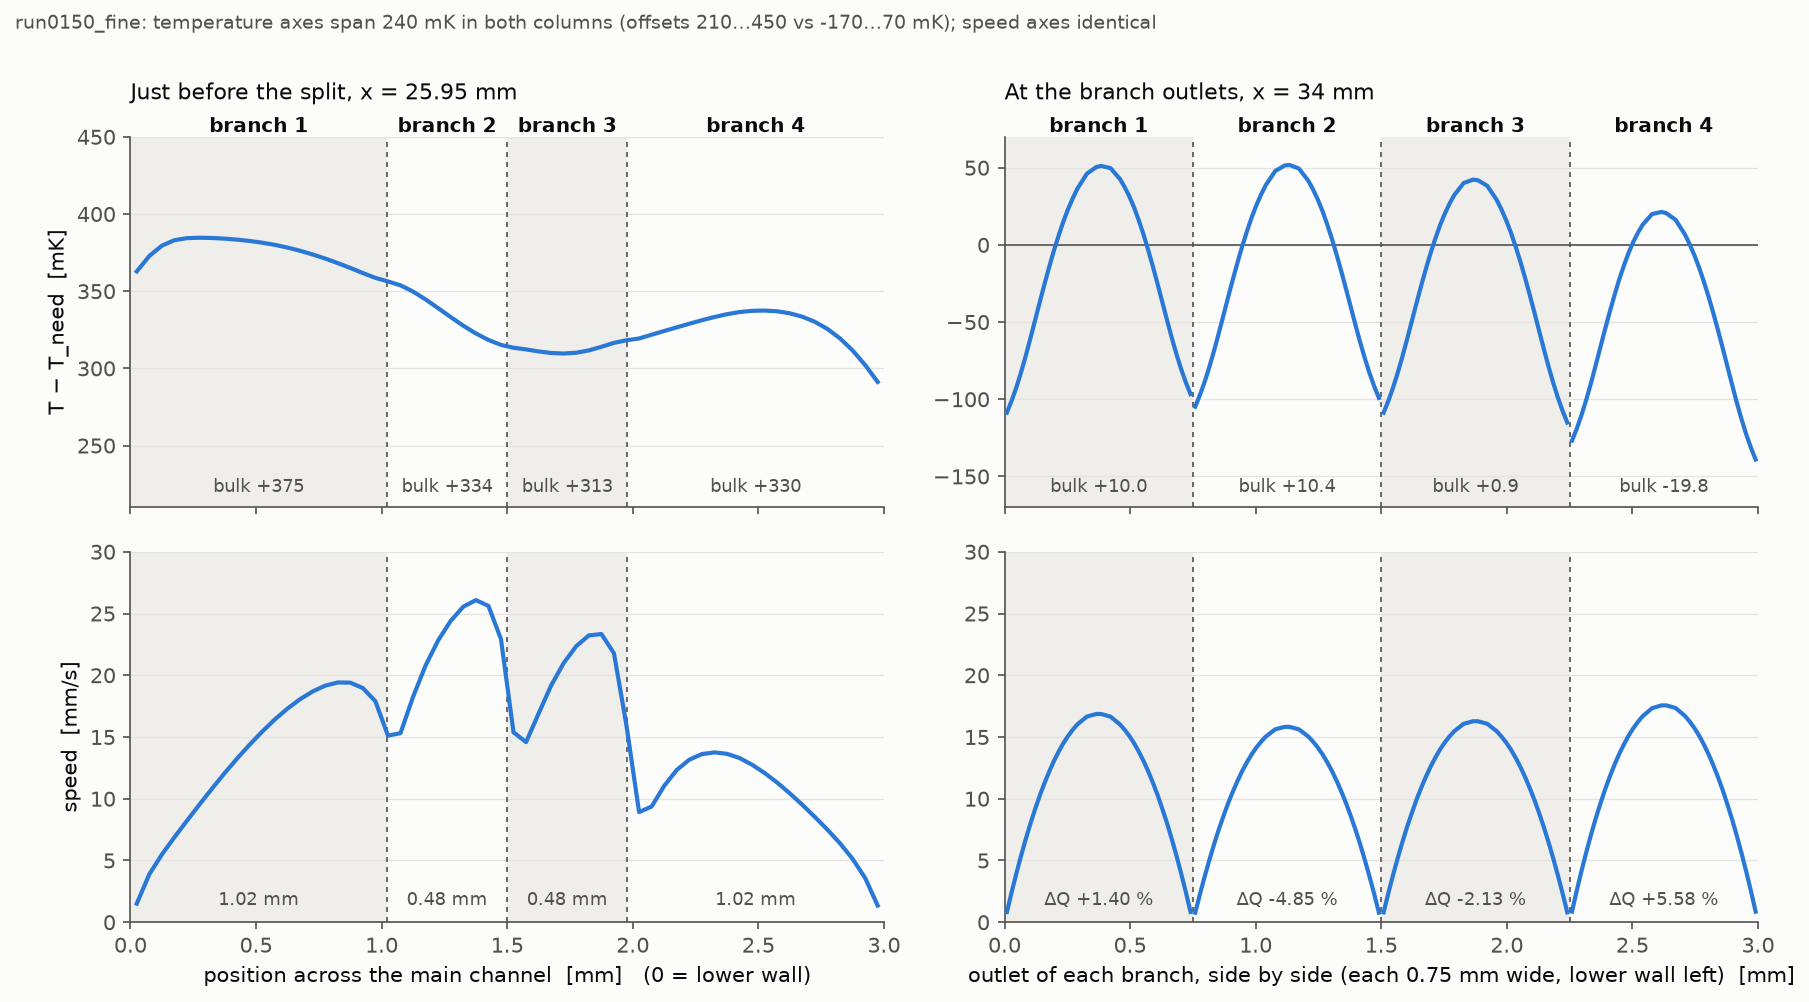
\includegraphics[width=0.9\textwidth]{runs/final_b2d_serp_presplit.png}
\caption{Cross-section just before the split of the same design, cut at the four branch inlets.}
\end{figure}

%=====================================================================
\section{Conclusions}
%=====================================================================
\begin{enumerate}
  \item At 6\,mL/min in a 3\mm{} channel, uniformity is set by how strongly the geometry folds the
        flow. Straight 980/756\mK{} (2D/3D, fully heated), best heater only 388/378\mK, sine
        120\mK, serpentine 6--12\mK{} (2D) and 27\mK{} (3D).
  \item Heat early and mix afterwards. Every optimum puts the heater at the inlet and leaves unheated
        bends or length after it. The heated length is short in the straight channel and
        medium-to-long in the serpentine; it is longest in 3D.
  \item With four branches the serpentine + straight design gives a 30\mK{} temperature spread,
        but a few percent flow imbalance. The straight channel with the analytic opening ratio gives
        the best flow balance but cannot equalize temperature.
  \item With two variables, BO and a grid reach the same valley. Coarse-mesh noise of up to
        1.7$\times$ decides which point inside it wins, so the final ranking must use several fine runs.
\end{enumerate}

\subsection*{Caveats}
\begin{itemize}
  \item In 3D and the branched serpentine the optimum is at a box bound ($\lambda$ min, $A$ max).
  \item The straight references sit at the short end of their heater sweeps. In 2D the 1.2\mm{}
        windows would need more than 99\,$^\circ$C; in 3D the 1.2\mm{} window (93\,$^\circ$C) is the
        shortest tried, so a shorter one may do slightly better.
  \item The branched results are 2D only; 3D secondary flow would change the jet at the fan.
  \item The 3D BO used only 28 coarse runs, and its coarse mesh reads about 30\,\% low.
\end{itemize}

%=====================================================================
\section{Files and how to reproduce}
%=====================================================================
\begin{itemize}
  \item \textbf{Case files:} \texttt{cases/final/*.yaml}, generated by \texttt{cases/final/make\_cases.py}.
  \item \textbf{Driver:} \texttt{scripts/run\_final\_study.sh}; logs in \texttt{runs/final\_logs/}.
  \item \textbf{Single runs:}
  \begin{itemize}
    \item BO: \texttt{.venv/bin/python -m comsol\_opt run cases/final/<case>.yaml}
    \item grid: \texttt{.venv/bin/python -m comsol\_opt.gridcase cases/final/<case>.yaml}
    \item 3D mesh check: \texttt{PYTHONPATH=. .venv/bin/python scripts/mesh\_check\_3d.py}
  \end{itemize}
  \item \textbf{Results:} \texttt{runs/final\_<case>[\_grid]/} (\texttt{history.jsonl}, \texttt{best.json},
        \texttt{fields/*.png}; the solved models \texttt{fields/*.mph} are not in the repository). Fully heated references:
        \texttt{runs/final\_u\{2,3\}d\_straight\_ref\_single/}. 3D mesh check: \texttt{runs/final\_u3d\_meshcheck/}.
  \item \textbf{This report:}
  \begin{itemize}
    \item figures: \texttt{report/make\_figs.py} and \texttt{report/make\_appendix.py};
    \item build: \texttt{tectonic report/report.tex}.
  \end{itemize}
\end{itemize}

\appendix
% generated by make_appendix.py
\section{Field plots of every run}\label{app:fields}
Every plot below is from the fine mesh. Unless noted, the design shown uses the best heater window found by the sweep. Files: \texttt{runs/<run>/fields/}.
\subsection{One outlet, 2D}
\clearpage
\subsubsection*{2D straight reference, fully heated (heater on the whole 24\mm)}
\noindent\texttt{runs/final\_u2d\_straight\_ref\_single}\par\medskip
\begin{figure}[H]\centering
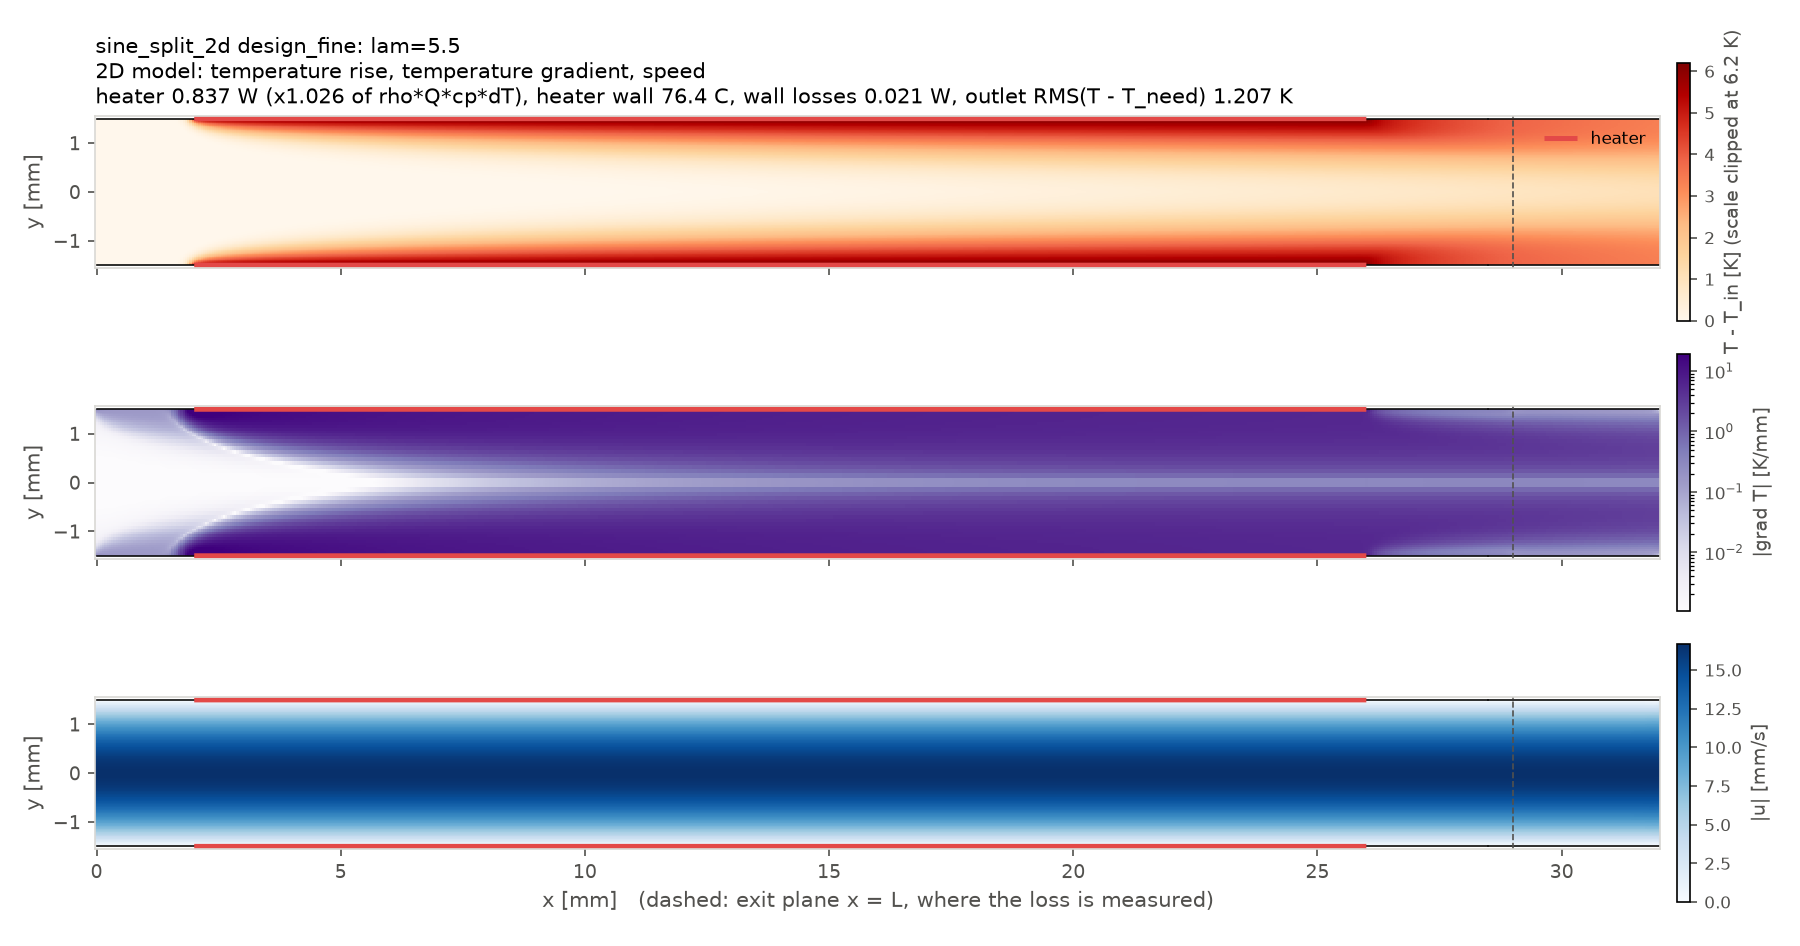
\includegraphics[width=0.95\textwidth,height=0.8\textheight,keepaspectratio]{runs/final_u2d_straight_ref_single_maps.png}
\caption{Temperature rise, temperature gradient and speed (mid-depth plane in 3D). Red: heated wall. The title's ``outlet RMS'' is the area-weighted $\ell_{2,\mathrm{area}}$.}
\end{figure}
\begin{figure}[H]\centering
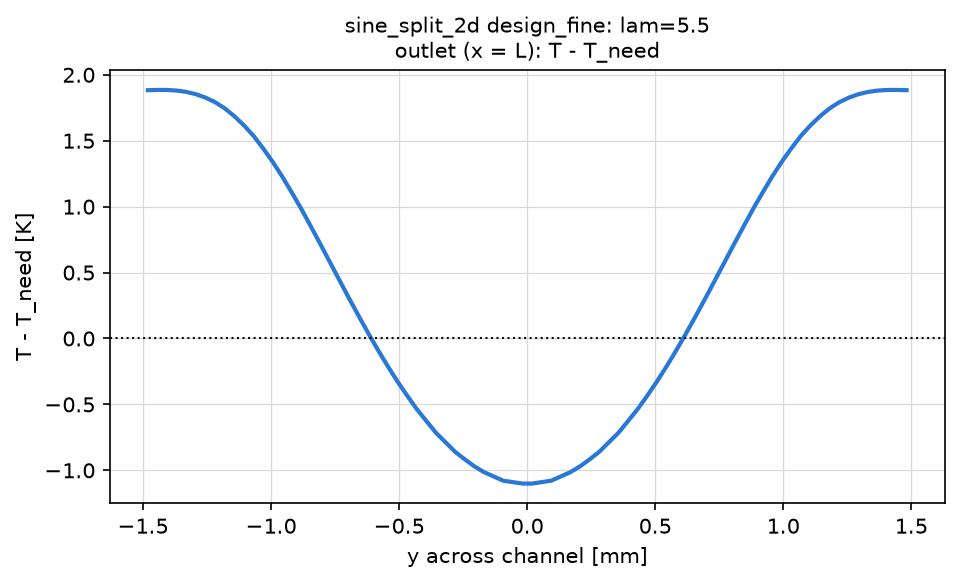
\includegraphics[width=0.75\textwidth,height=0.8\textheight,keepaspectratio]{runs/final_u2d_straight_ref_single_outlet.png}
\caption{Outlet temperature (and, in 3D, the outlet plane).}
\end{figure}
\begin{figure}[H]\centering
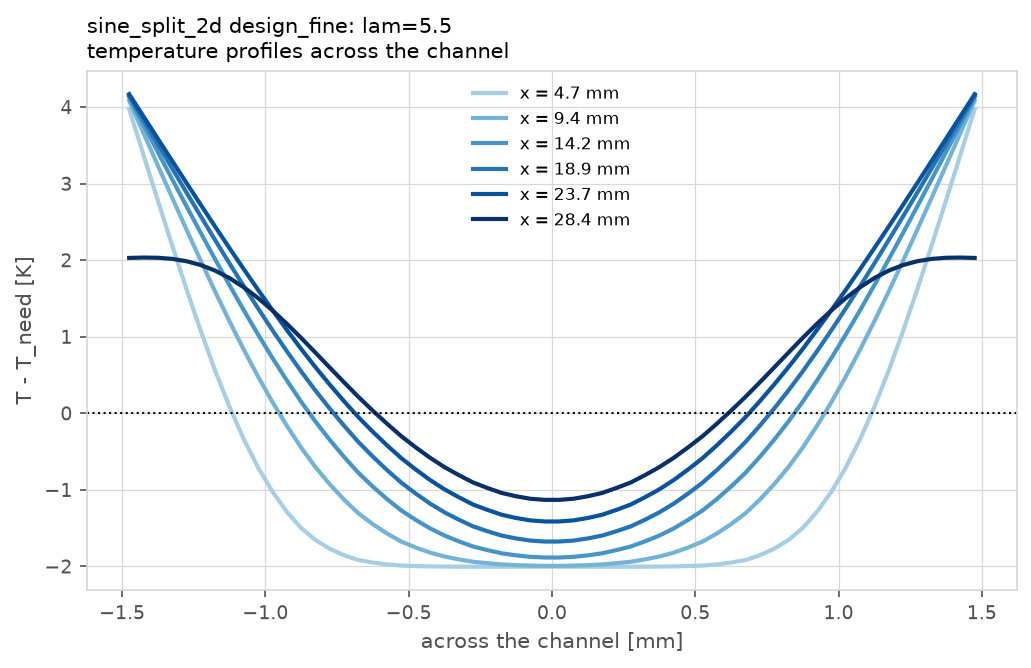
\includegraphics[width=0.62\textwidth,height=0.8\textheight,keepaspectratio]{runs/final_u2d_straight_ref_single_slices.png}
\caption{Temperature profiles across the channel at several $x$ stations.}
\end{figure}
\begin{figure}[H]\centering
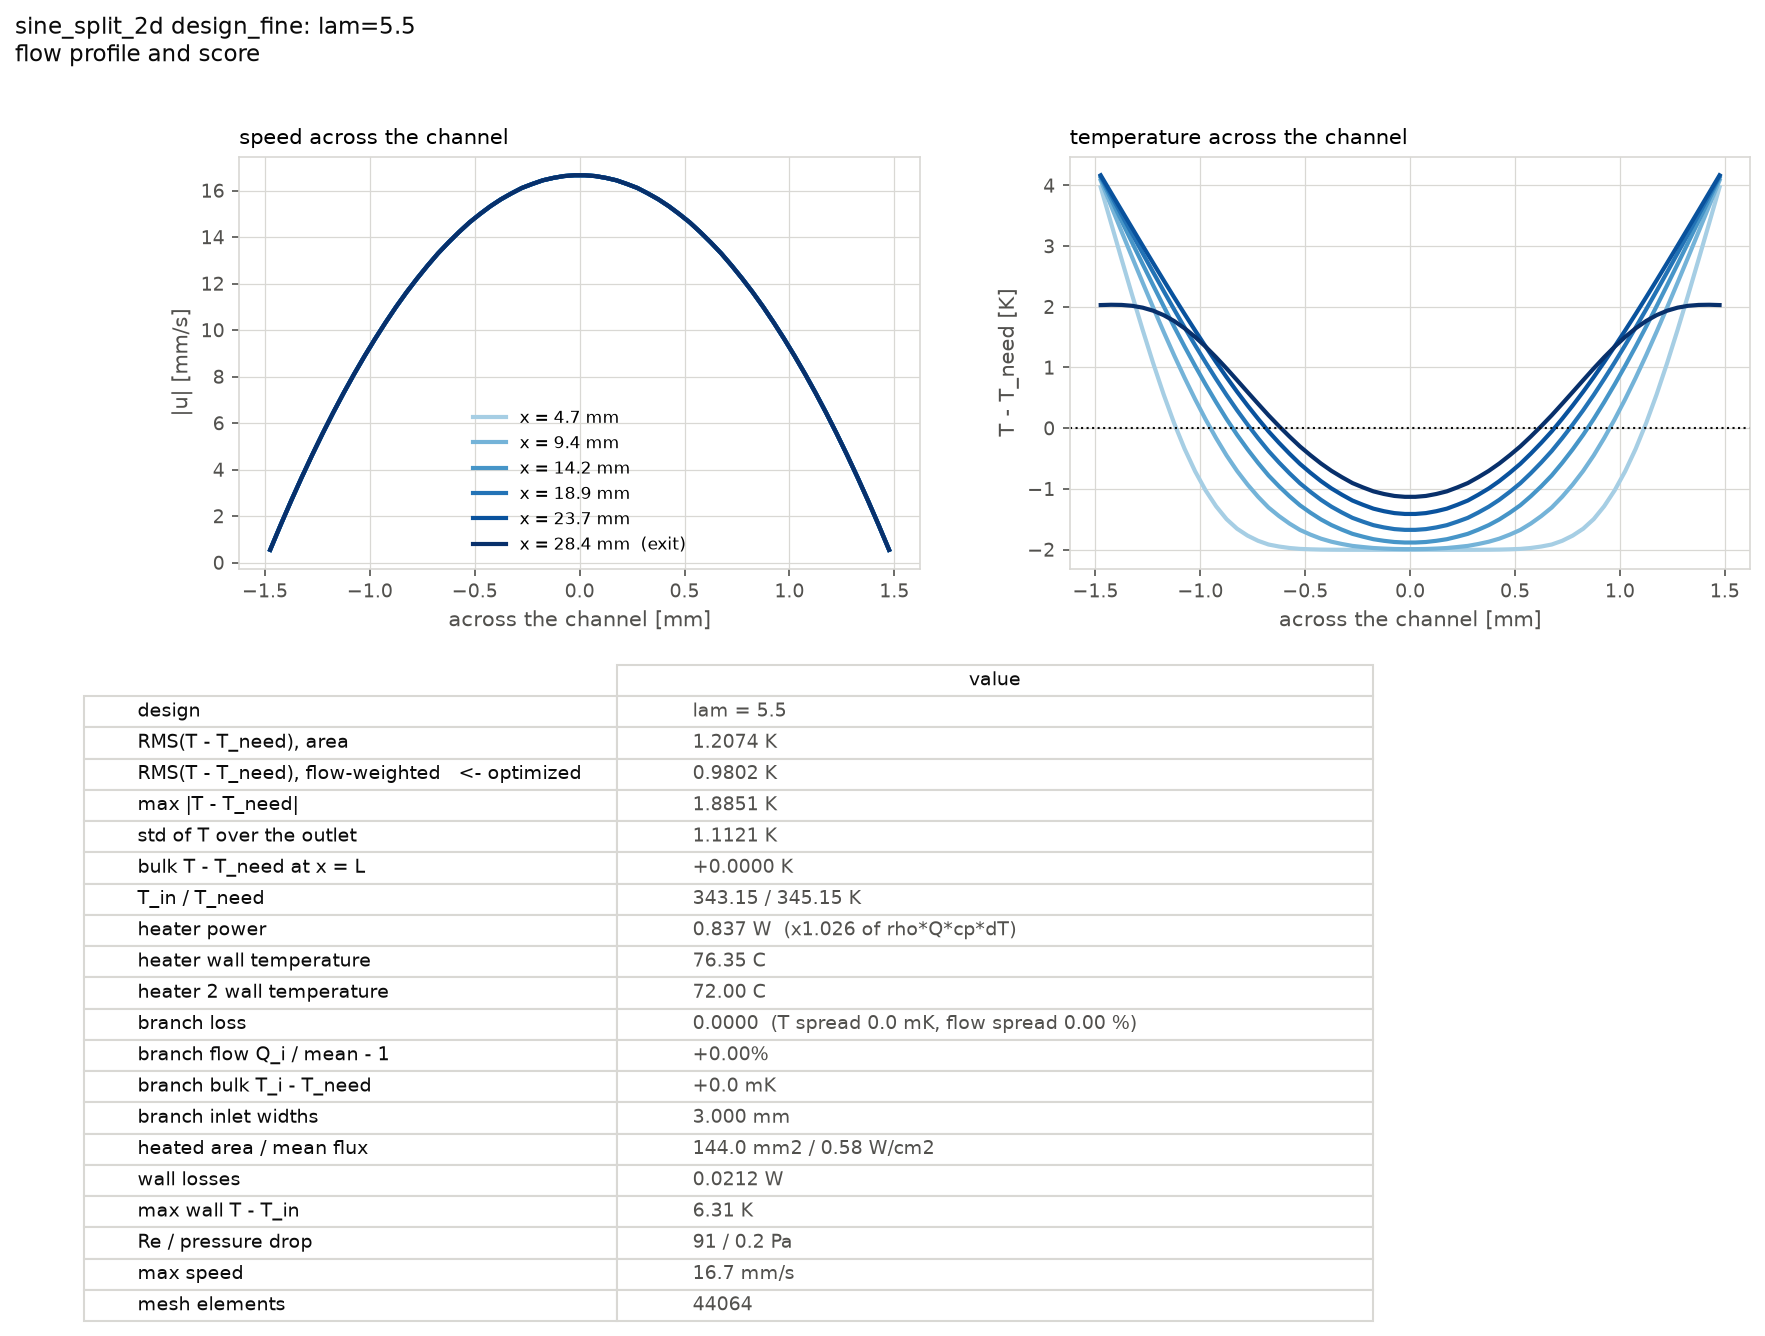
\includegraphics[width=0.8\textwidth,height=0.8\textheight,keepaspectratio]{runs/final_u2d_straight_ref_single_profile.png}
\caption{Speed and temperature across the channel at several $x$ stations, and the full score table of the design.}
\end{figure}
\begin{figure}[H]\centering
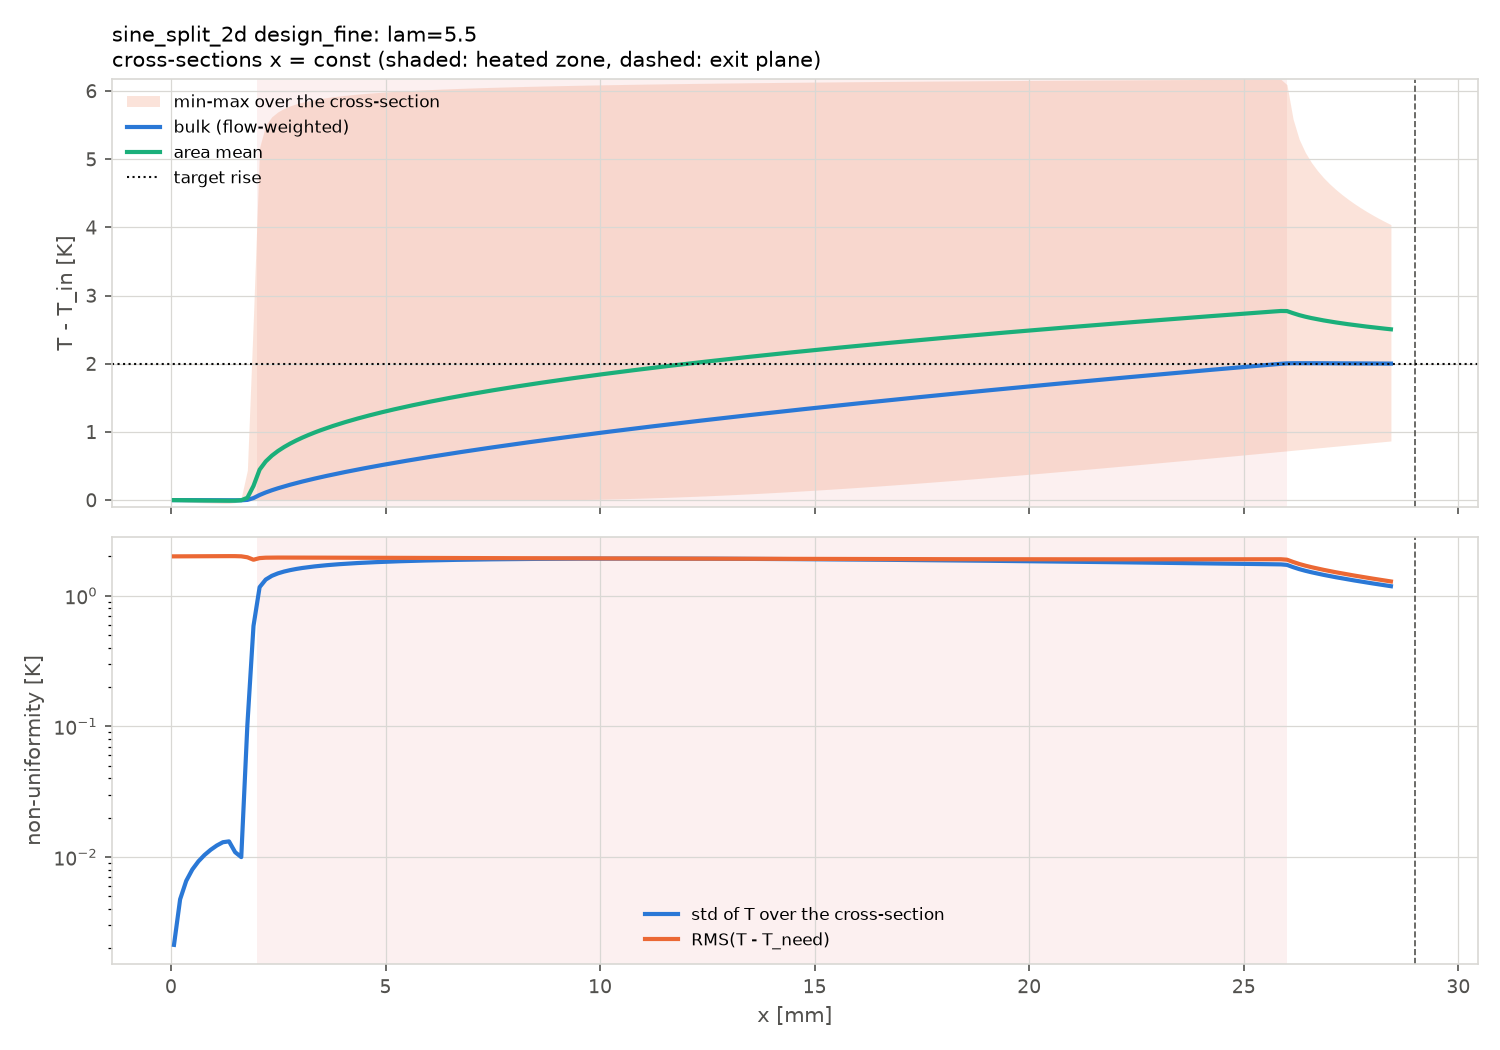
\includegraphics[width=0.8\textwidth,height=0.8\textheight,keepaspectratio]{runs/final_u2d_straight_ref_single_along_x.png}
\caption{Bulk, mean, min and max temperature along the channel.}
\end{figure}
\clearpage
\subsubsection*{2D straight reference, best heater window (start 0, length 10\,\%): 388\mK}
\noindent\texttt{runs/final\_u2d\_straight\_ref}\par\medskip
\begin{figure}[H]\centering
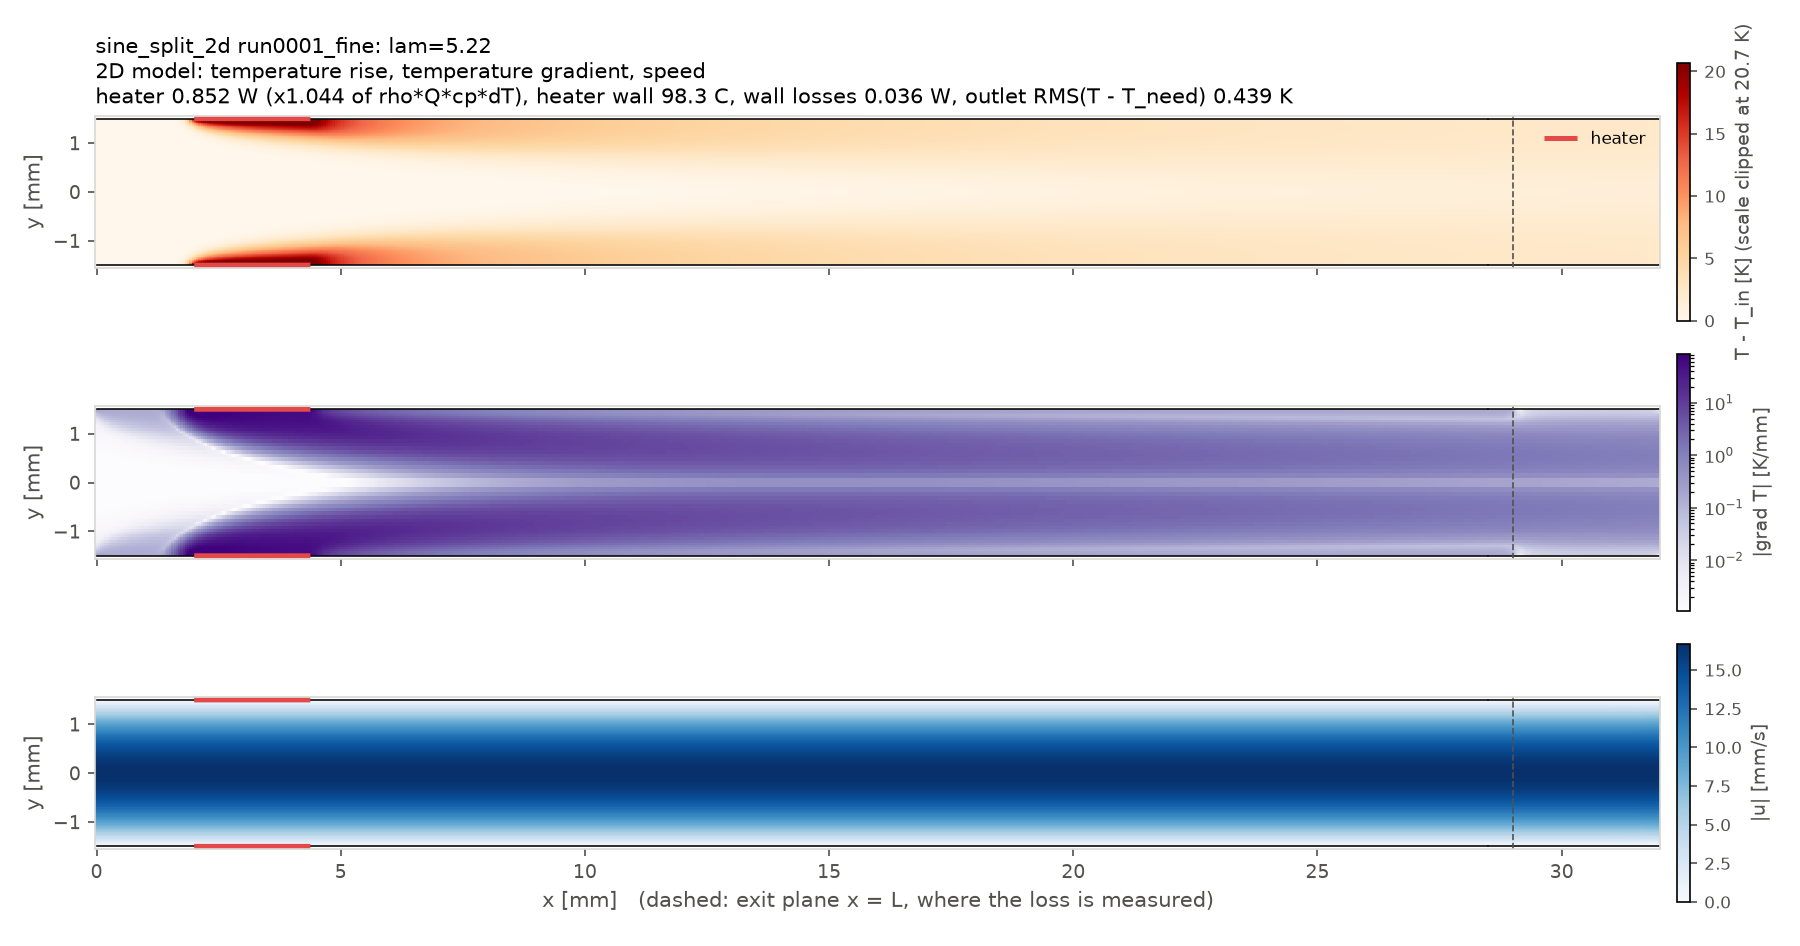
\includegraphics[width=0.95\textwidth,height=0.8\textheight,keepaspectratio]{runs/final_u2d_straight_ref_maps.png}
\caption{Temperature rise, temperature gradient and speed (mid-depth plane in 3D). Red: heated wall. The title's ``outlet RMS'' is the area-weighted $\ell_{2,\mathrm{area}}$.}
\end{figure}
\begin{figure}[H]\centering
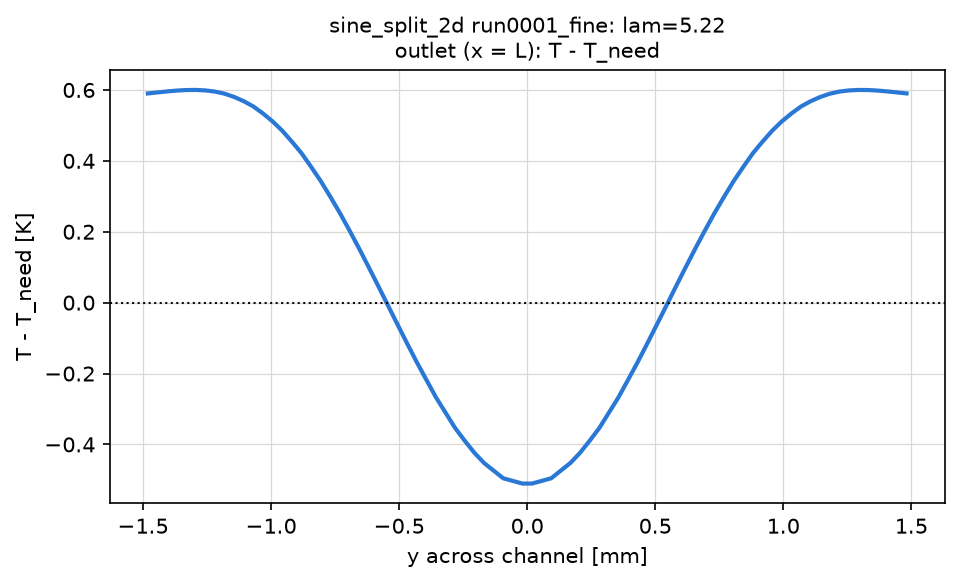
\includegraphics[width=0.75\textwidth,height=0.8\textheight,keepaspectratio]{runs/final_u2d_straight_ref_outlet.png}
\caption{Outlet temperature (and, in 3D, the outlet plane).}
\end{figure}
\begin{figure}[H]\centering
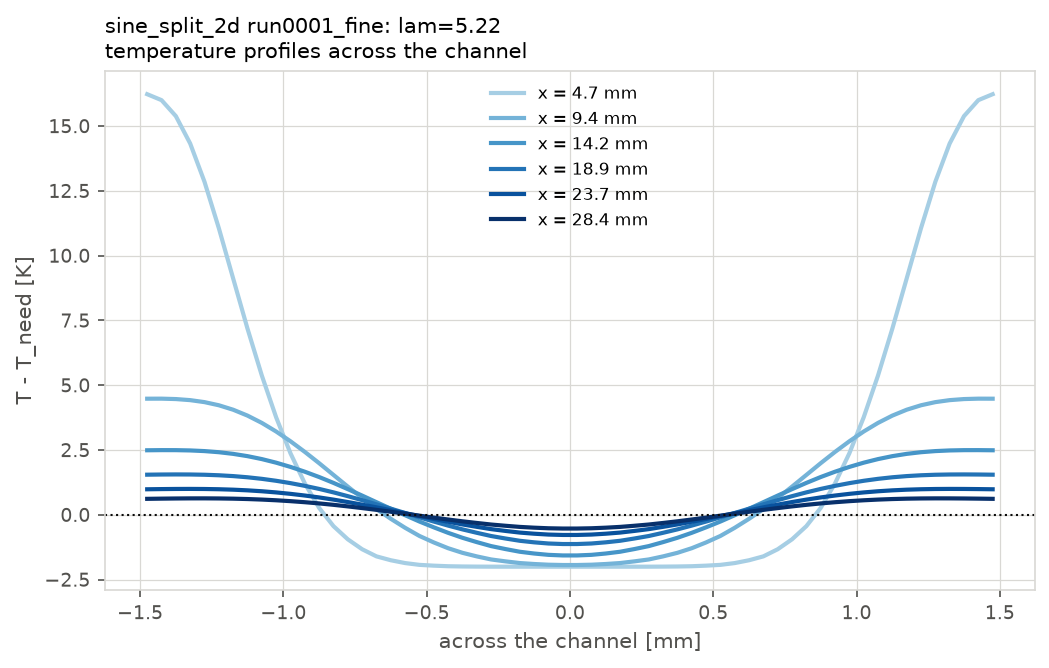
\includegraphics[width=0.62\textwidth,height=0.8\textheight,keepaspectratio]{runs/final_u2d_straight_ref_slices.png}
\caption{Temperature profiles across the channel at several $x$ stations.}
\end{figure}
\begin{figure}[H]\centering
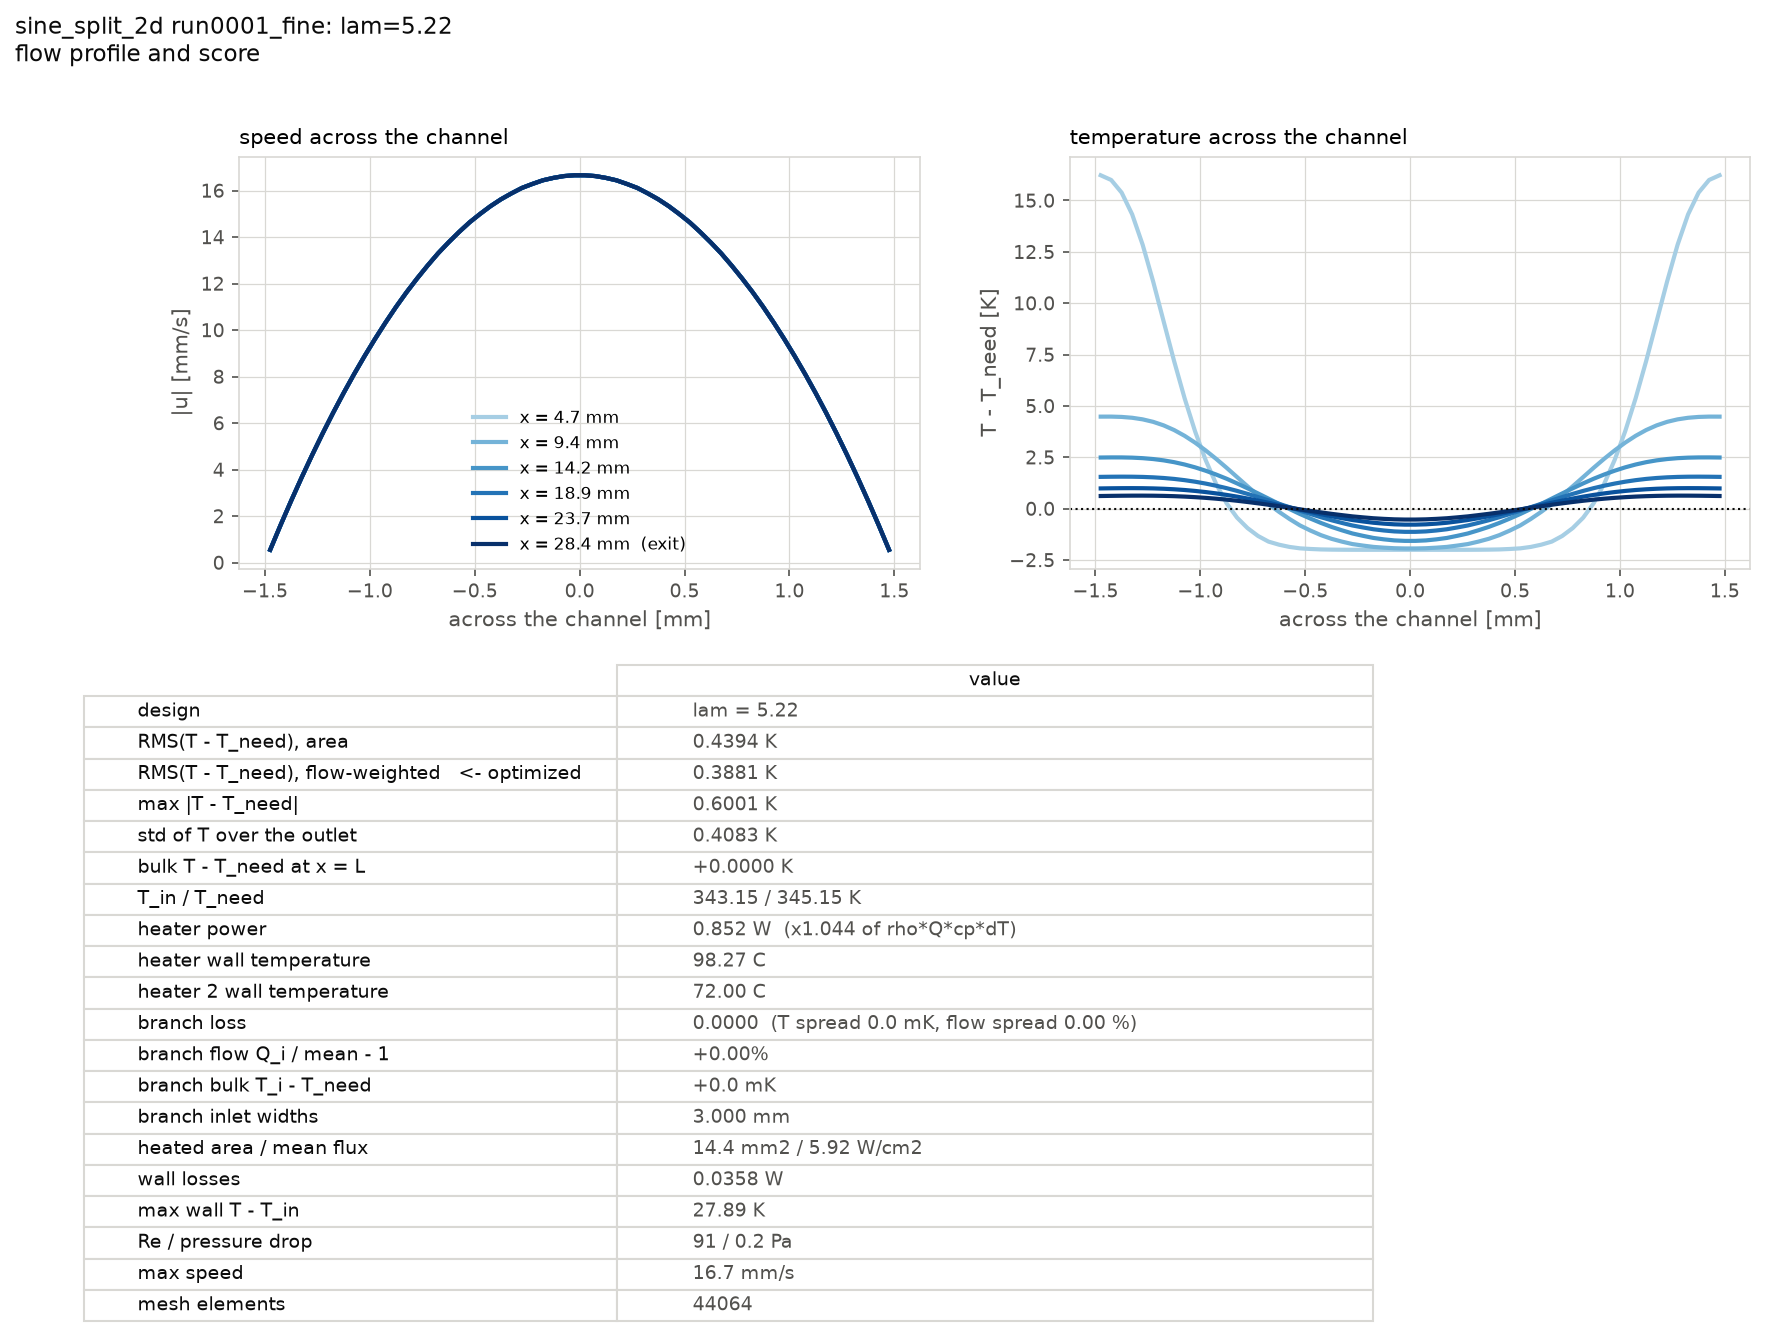
\includegraphics[width=0.8\textwidth,height=0.8\textheight,keepaspectratio]{runs/final_u2d_straight_ref_profile.png}
\caption{Speed and temperature across the channel at several $x$ stations, and the full score table of the design.}
\end{figure}
\begin{figure}[H]\centering
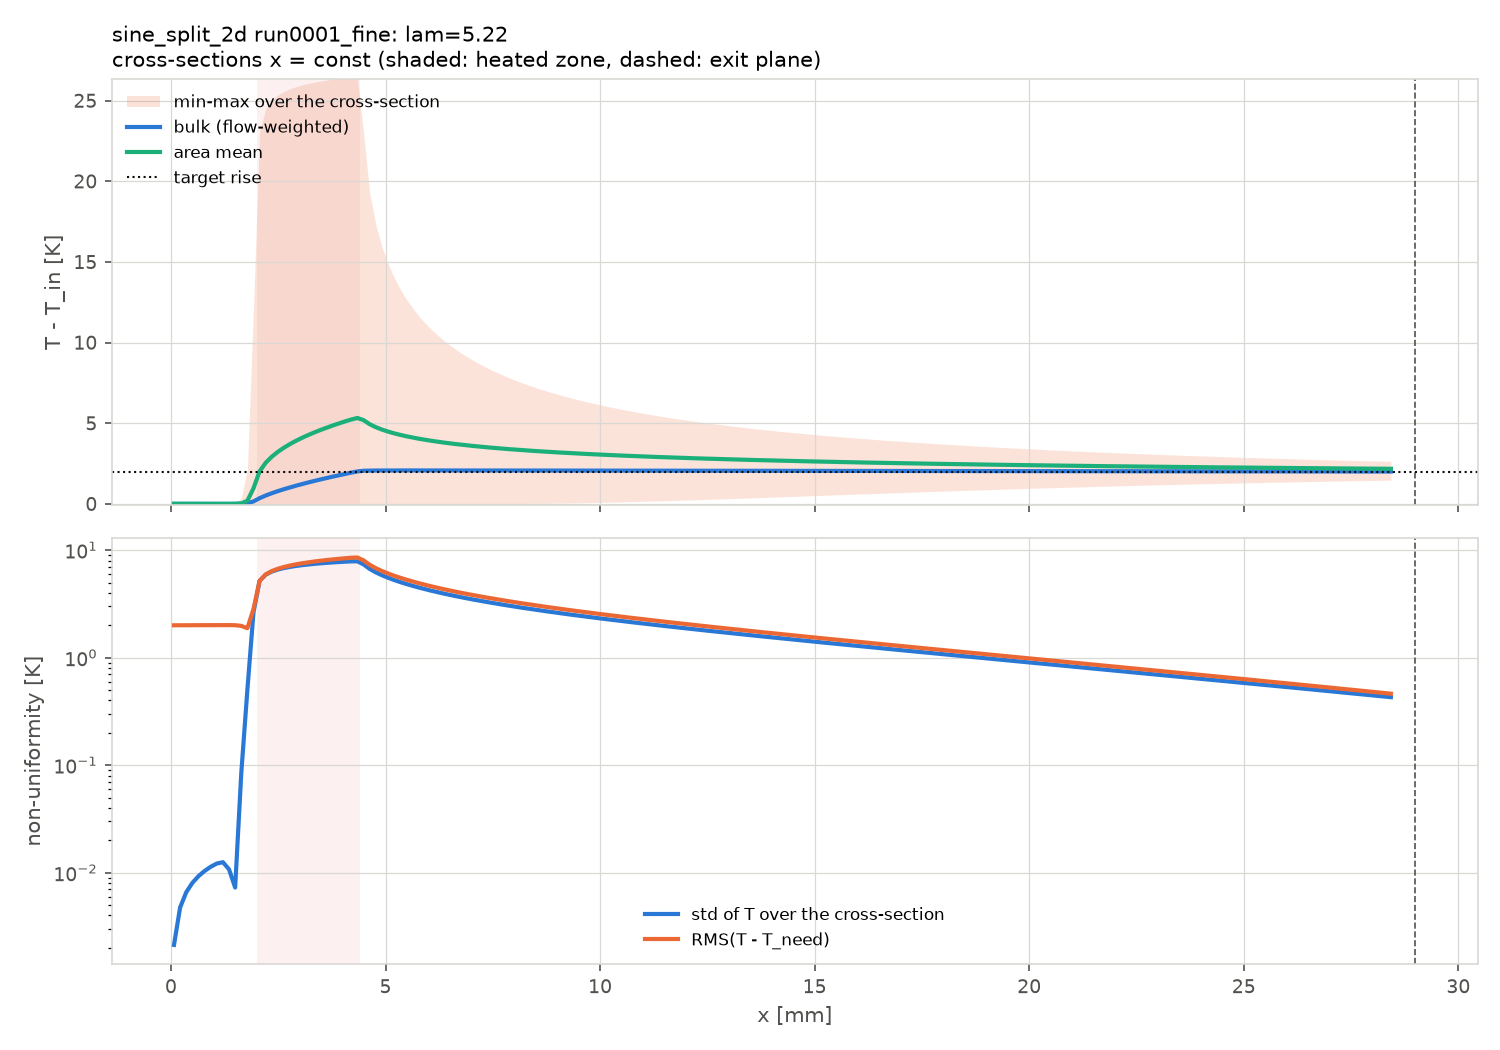
\includegraphics[width=0.8\textwidth,height=0.8\textheight,keepaspectratio]{runs/final_u2d_straight_ref_along_x.png}
\caption{Bulk, mean, min and max temperature along the channel.}
\end{figure}
\clearpage
\subsubsection*{2D sine, BO best \#50 ($\lambda$ 11.14, $a$ 1, heater 30\,\%): 120\mK}
\noindent\texttt{runs/final\_u2d\_sine}\par\medskip
\begin{figure}[H]\centering
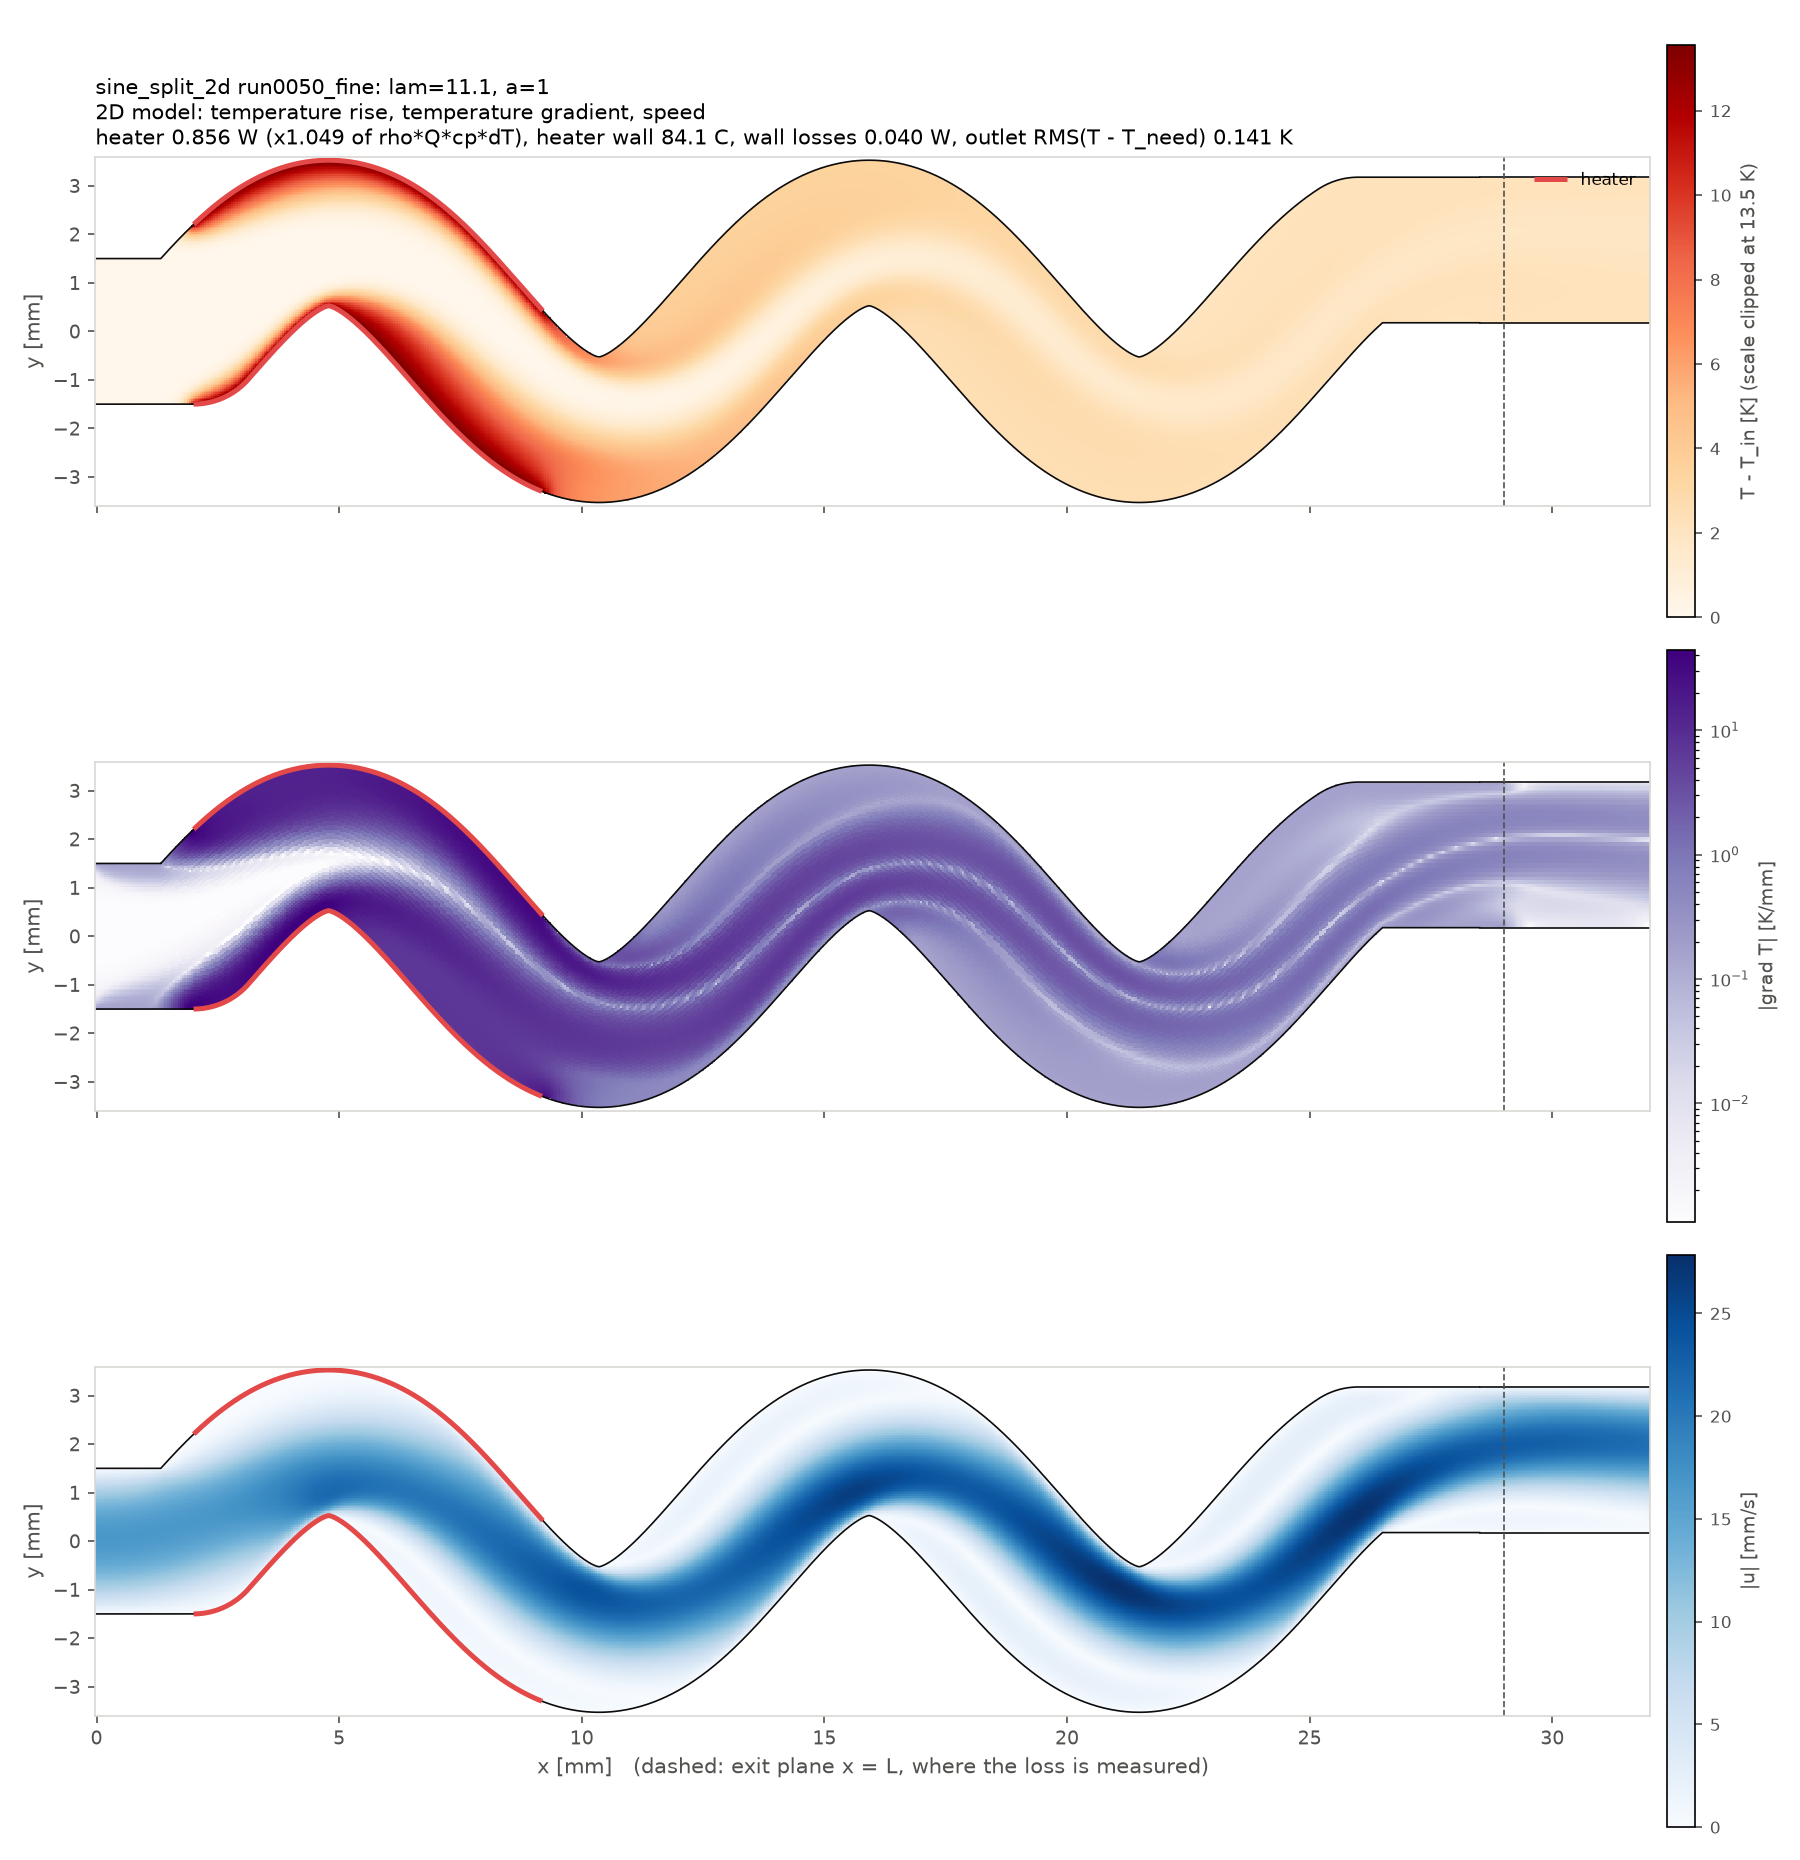
\includegraphics[width=0.95\textwidth,height=0.8\textheight,keepaspectratio]{runs/final_u2d_sine_maps.png}
\caption{Temperature rise, temperature gradient and speed (mid-depth plane in 3D). Red: heated wall. The title's ``outlet RMS'' is the area-weighted $\ell_{2,\mathrm{area}}$.}
\end{figure}
\begin{figure}[H]\centering
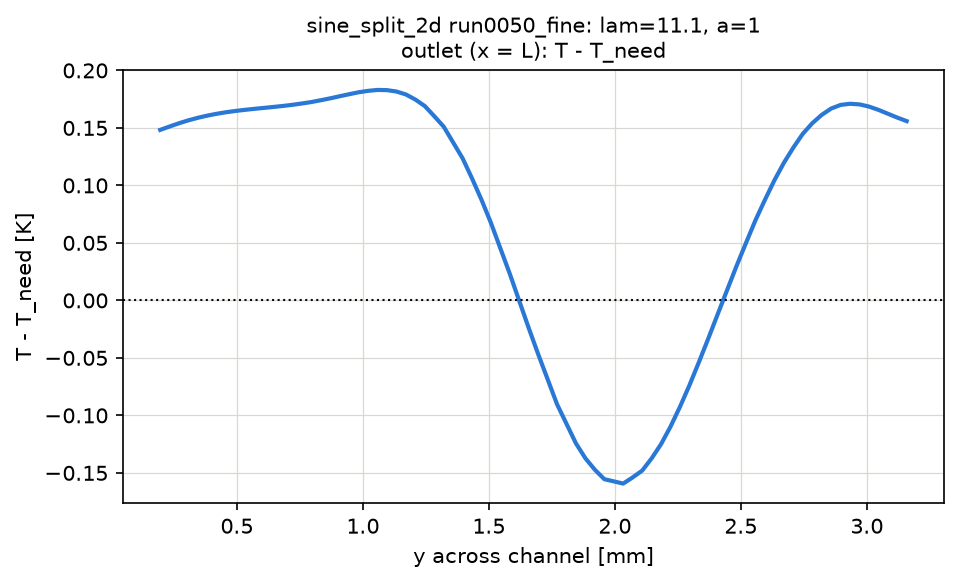
\includegraphics[width=0.75\textwidth,height=0.8\textheight,keepaspectratio]{runs/final_u2d_sine_outlet.png}
\caption{Outlet temperature (and, in 3D, the outlet plane).}
\end{figure}
\begin{figure}[H]\centering
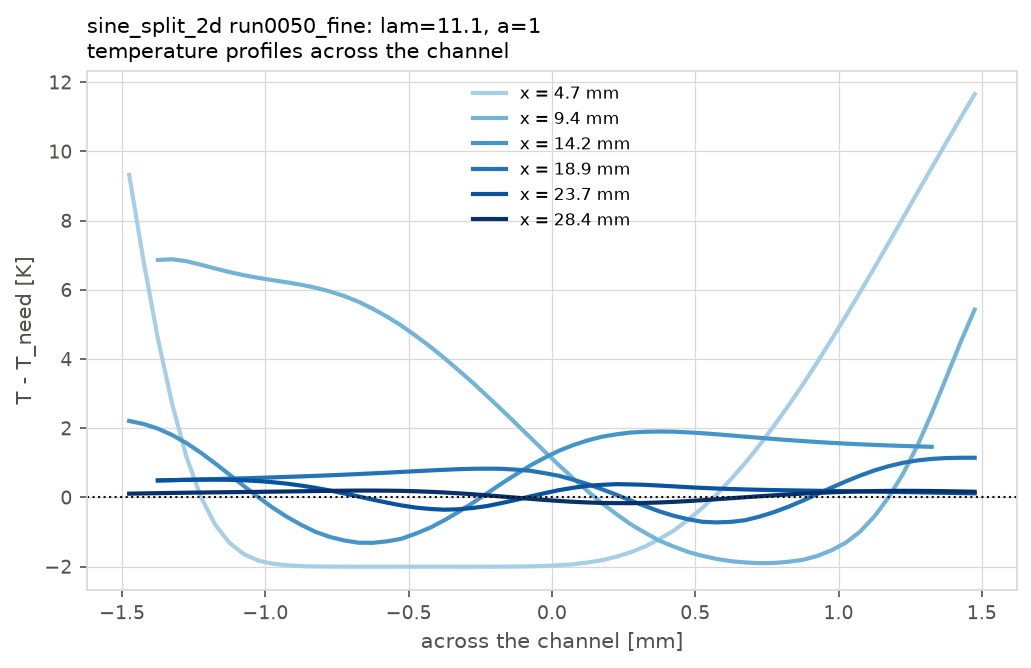
\includegraphics[width=0.62\textwidth,height=0.8\textheight,keepaspectratio]{runs/final_u2d_sine_slices.png}
\caption{Temperature profiles across the channel at several $x$ stations.}
\end{figure}
\begin{figure}[H]\centering
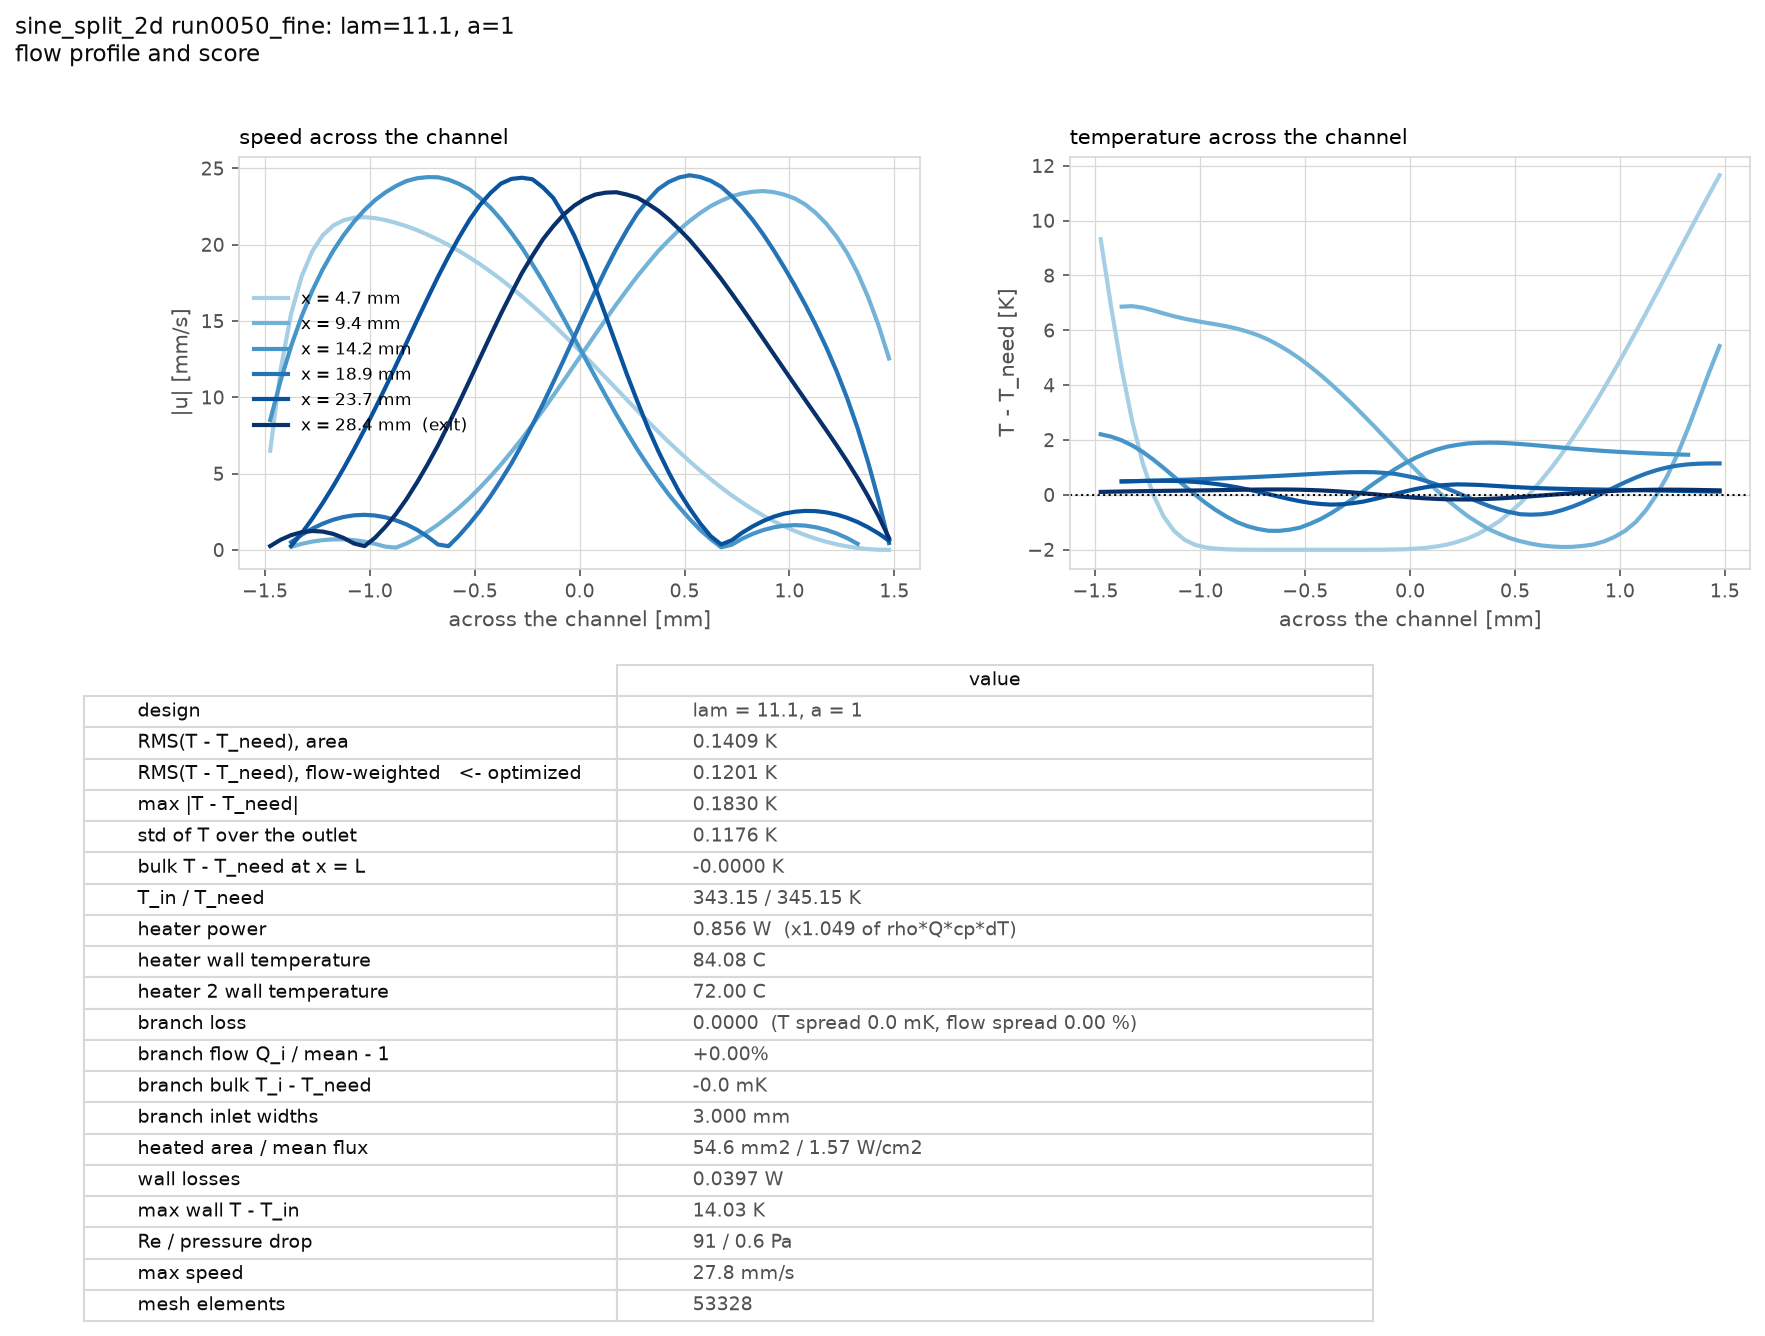
\includegraphics[width=0.8\textwidth,height=0.8\textheight,keepaspectratio]{runs/final_u2d_sine_profile.png}
\caption{Speed and temperature across the channel at several $x$ stations, and the full score table of the design.}
\end{figure}
\begin{figure}[H]\centering
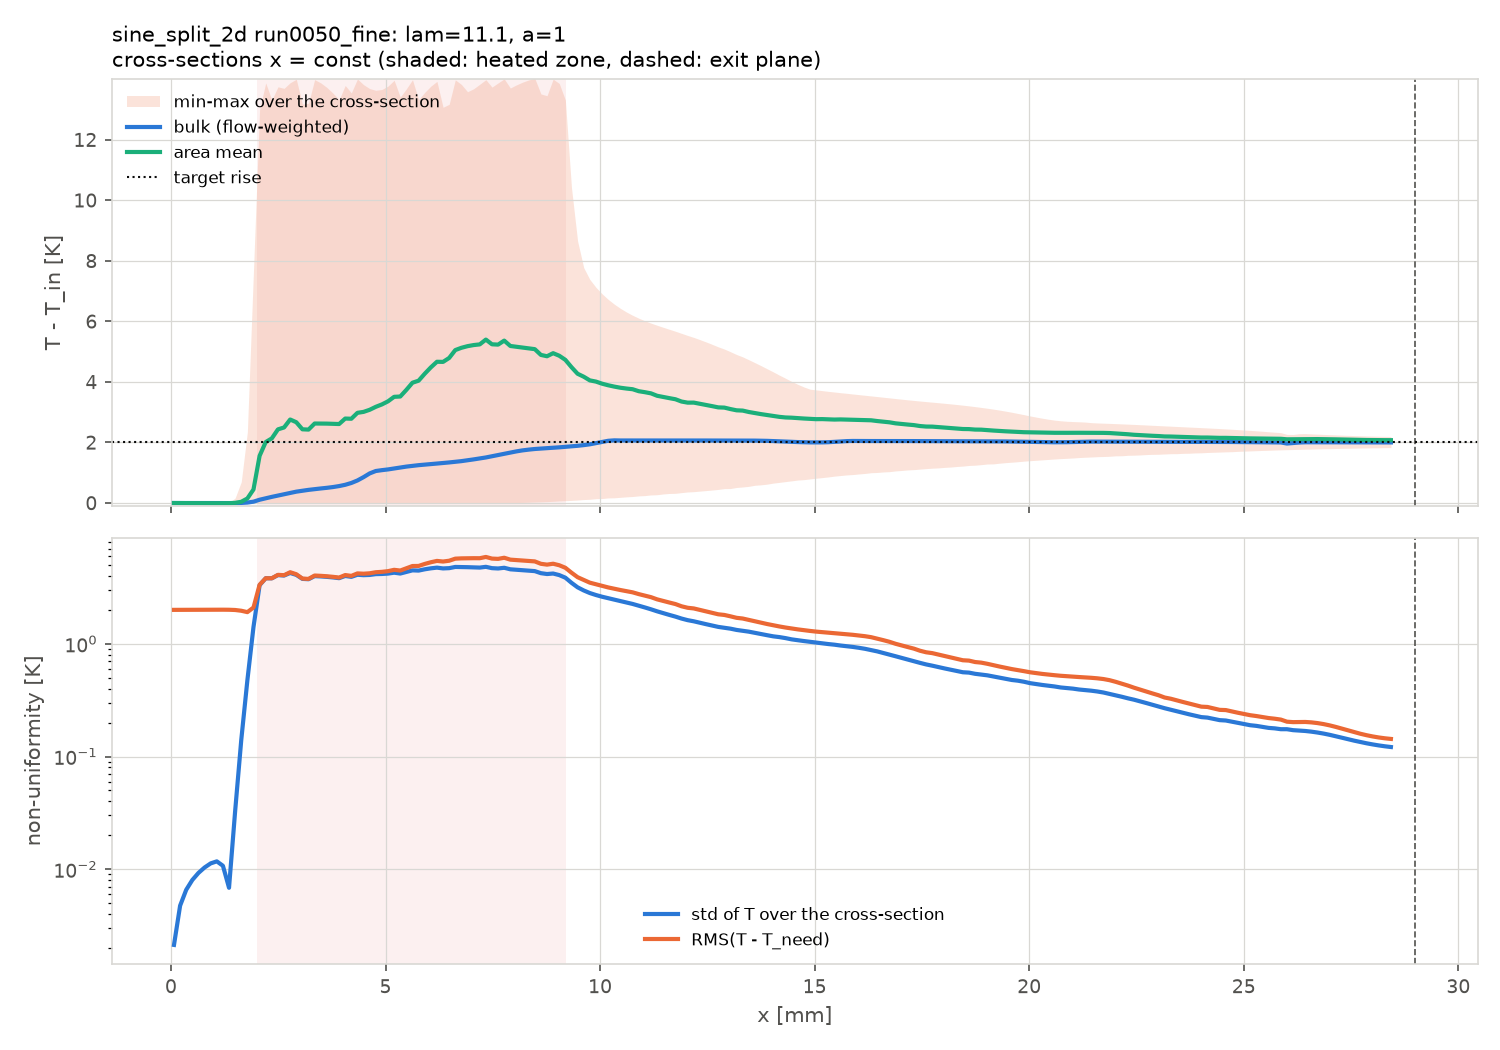
\includegraphics[width=0.8\textwidth,height=0.8\textheight,keepaspectratio]{runs/final_u2d_sine_along_x.png}
\caption{Bulk, mean, min and max temperature along the channel.}
\end{figure}
\begin{figure}[H]\centering
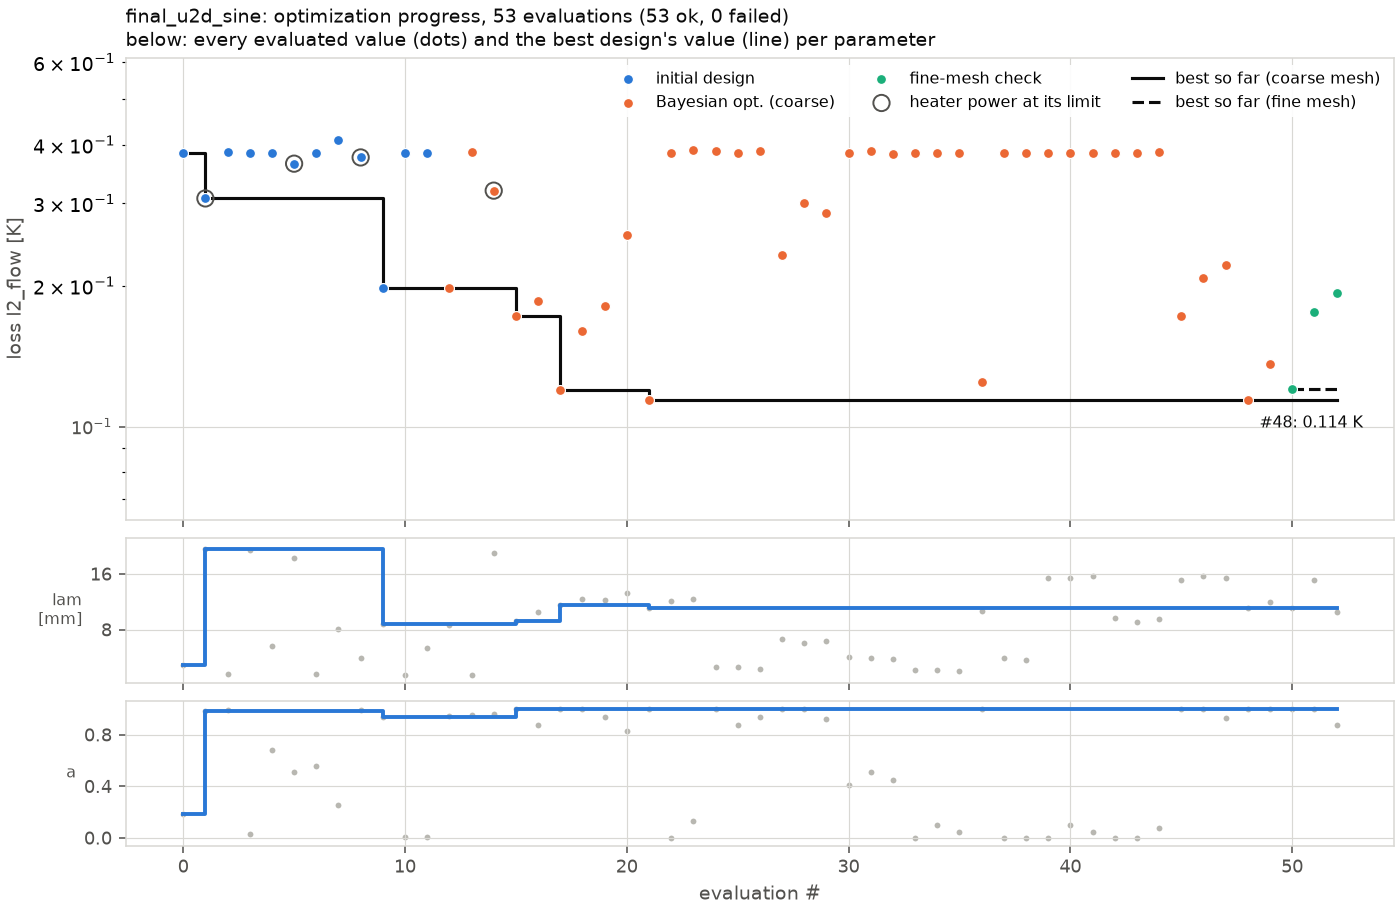
\includegraphics[width=0.85\textwidth]{runs/final_u2d_sine_progress_loss.png}
\caption{Search history: loss of every evaluation, best so far, and the parameters.}
\end{figure}
\clearpage
\subsubsection*{2D sine, grid best \#112 ($\lambda$ 11.10, $a$ 1, heater 30\,\%): 120\mK}
\noindent\texttt{runs/final\_u2d\_sine\_grid}\par\medskip
\begin{figure}[H]\centering
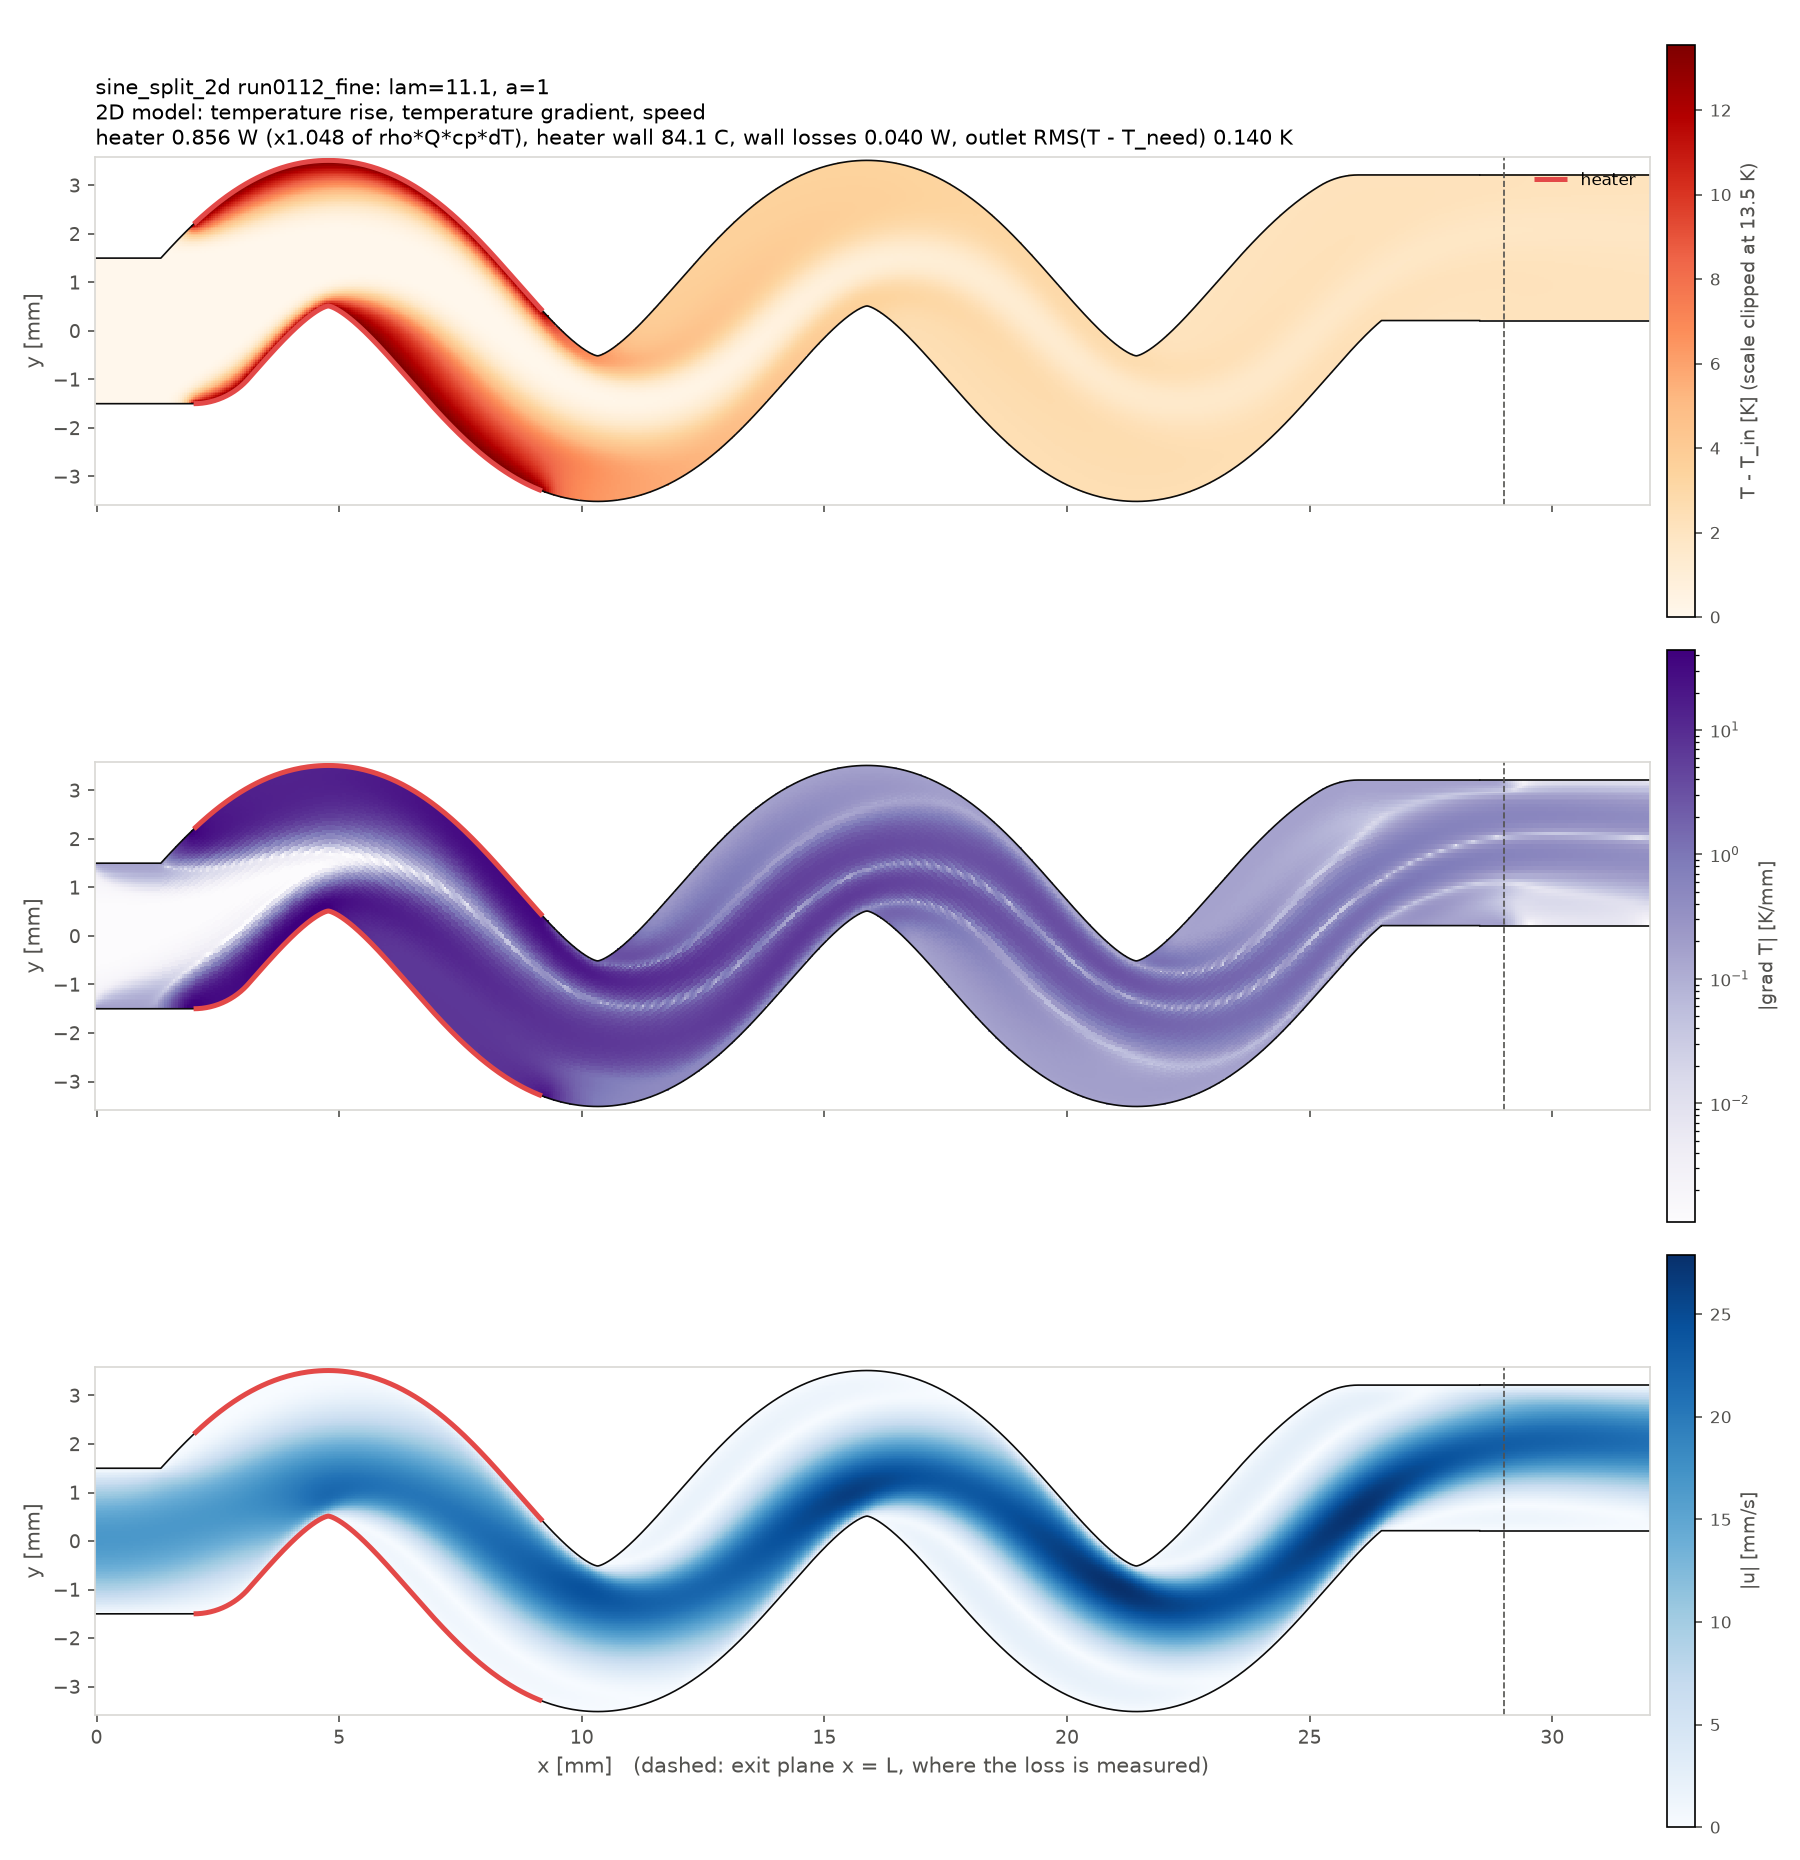
\includegraphics[width=0.95\textwidth,height=0.8\textheight,keepaspectratio]{runs/final_u2d_sine_grid_maps.png}
\caption{Temperature rise, temperature gradient and speed (mid-depth plane in 3D). Red: heated wall. The title's ``outlet RMS'' is the area-weighted $\ell_{2,\mathrm{area}}$.}
\end{figure}
\begin{figure}[H]\centering
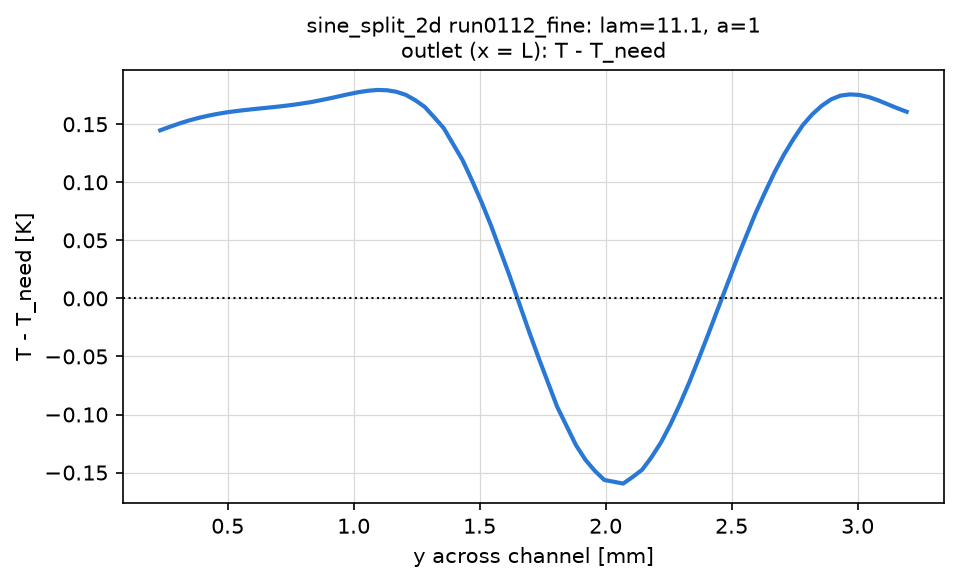
\includegraphics[width=0.75\textwidth,height=0.8\textheight,keepaspectratio]{runs/final_u2d_sine_grid_outlet.png}
\caption{Outlet temperature (and, in 3D, the outlet plane).}
\end{figure}
\begin{figure}[H]\centering
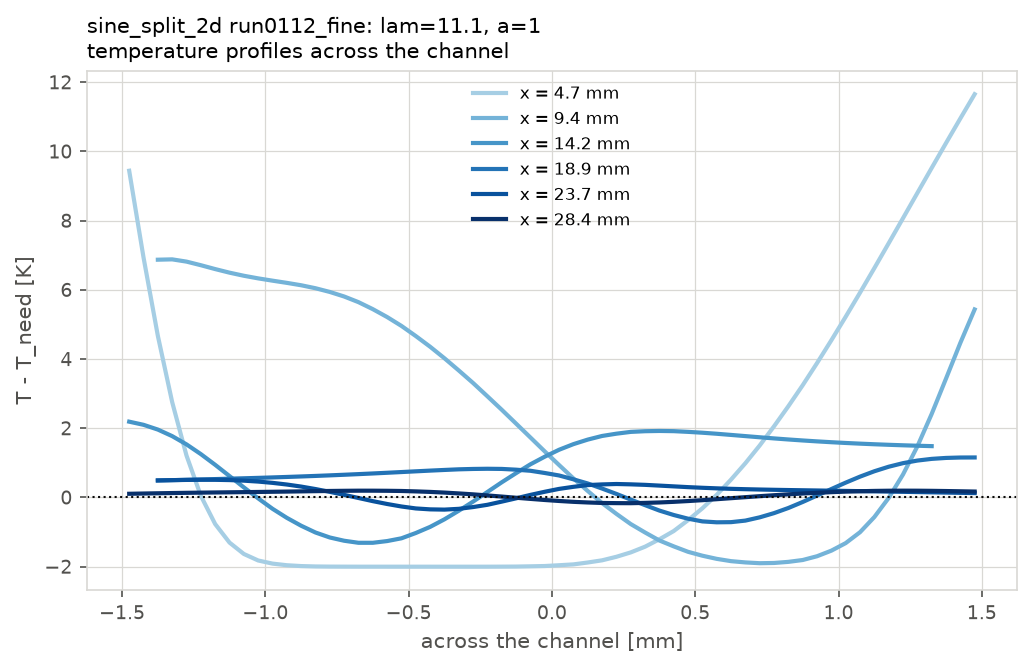
\includegraphics[width=0.62\textwidth,height=0.8\textheight,keepaspectratio]{runs/final_u2d_sine_grid_slices.png}
\caption{Temperature profiles across the channel at several $x$ stations.}
\end{figure}
\begin{figure}[H]\centering
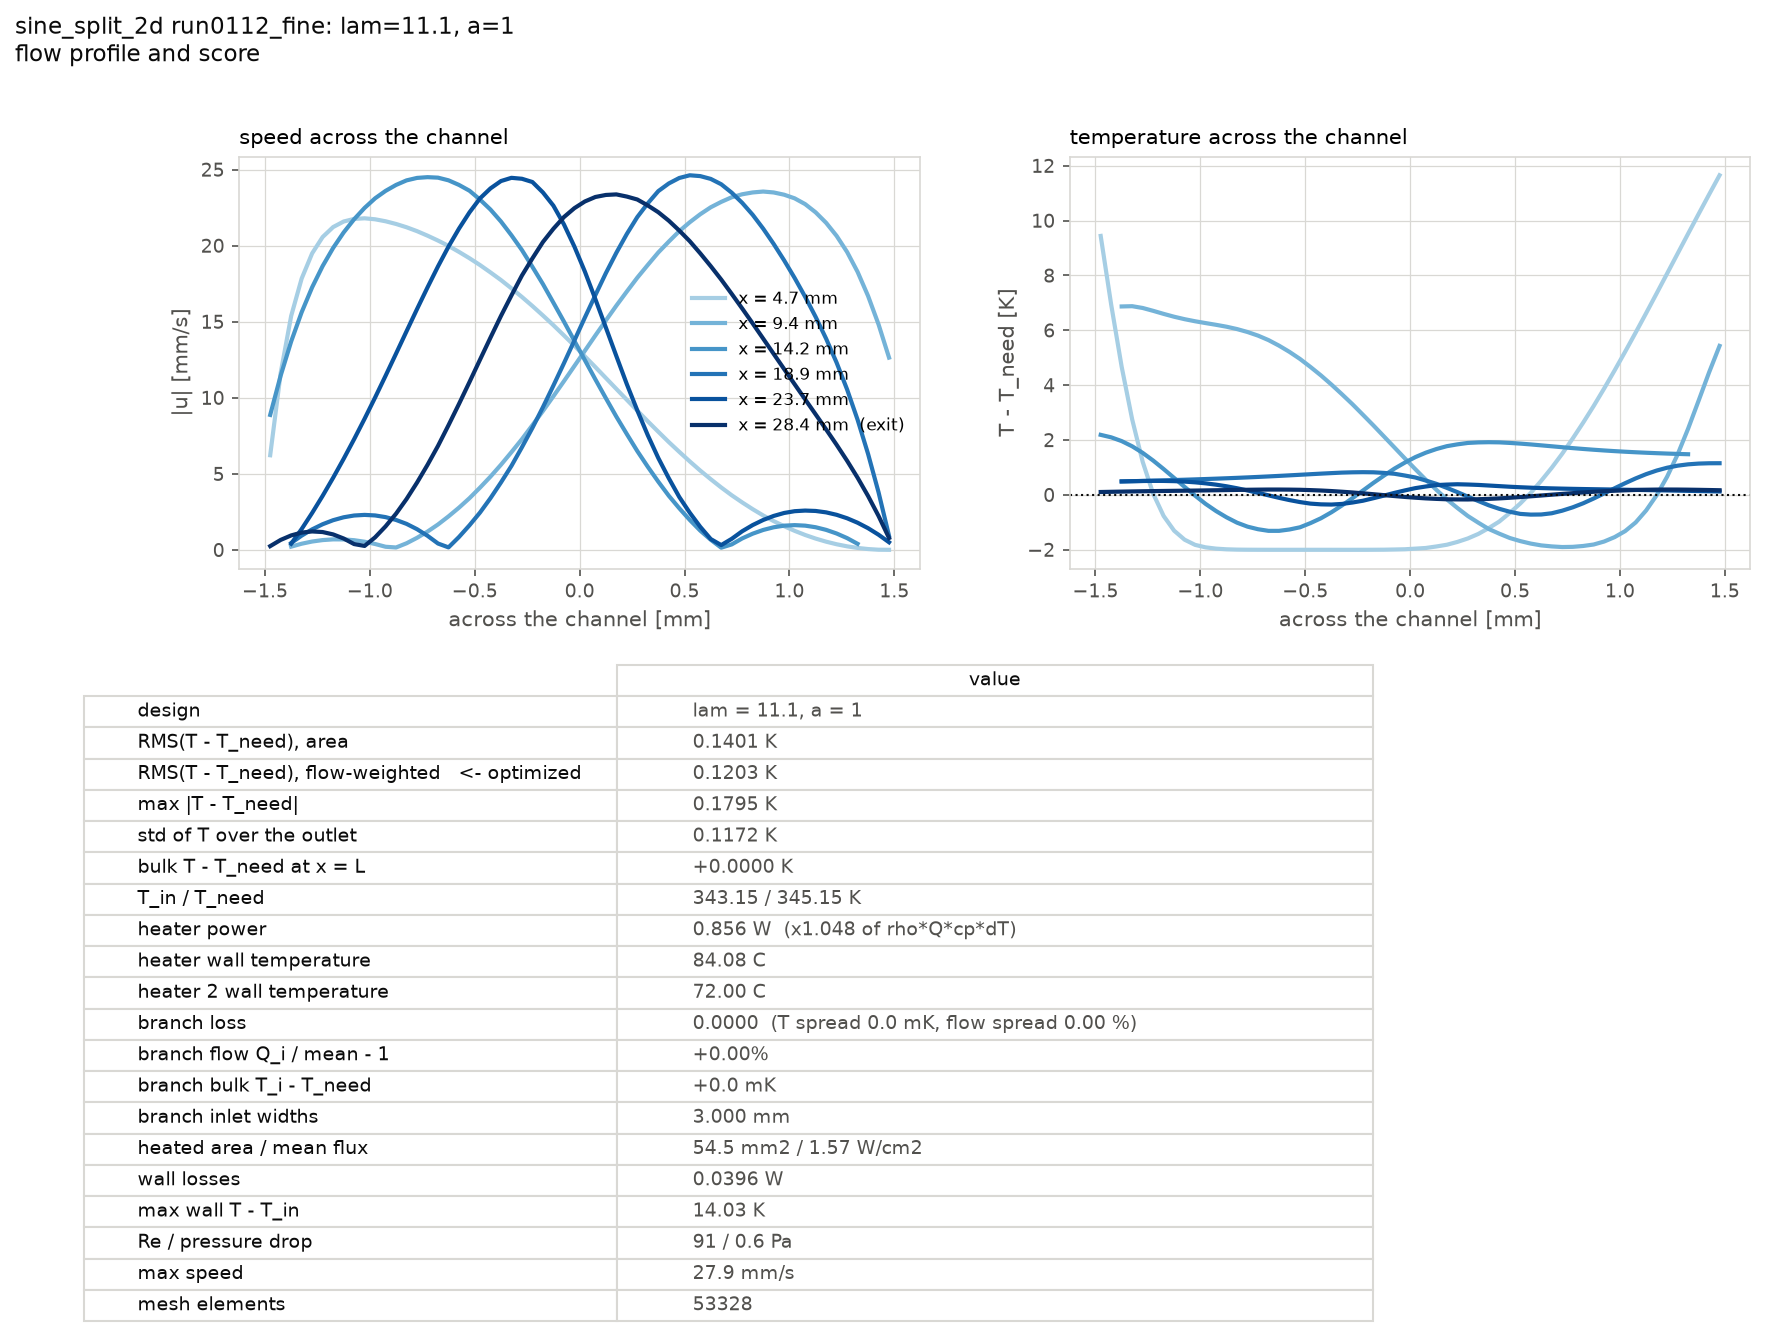
\includegraphics[width=0.8\textwidth,height=0.8\textheight,keepaspectratio]{runs/final_u2d_sine_grid_profile.png}
\caption{Speed and temperature across the channel at several $x$ stations, and the full score table of the design.}
\end{figure}
\begin{figure}[H]\centering
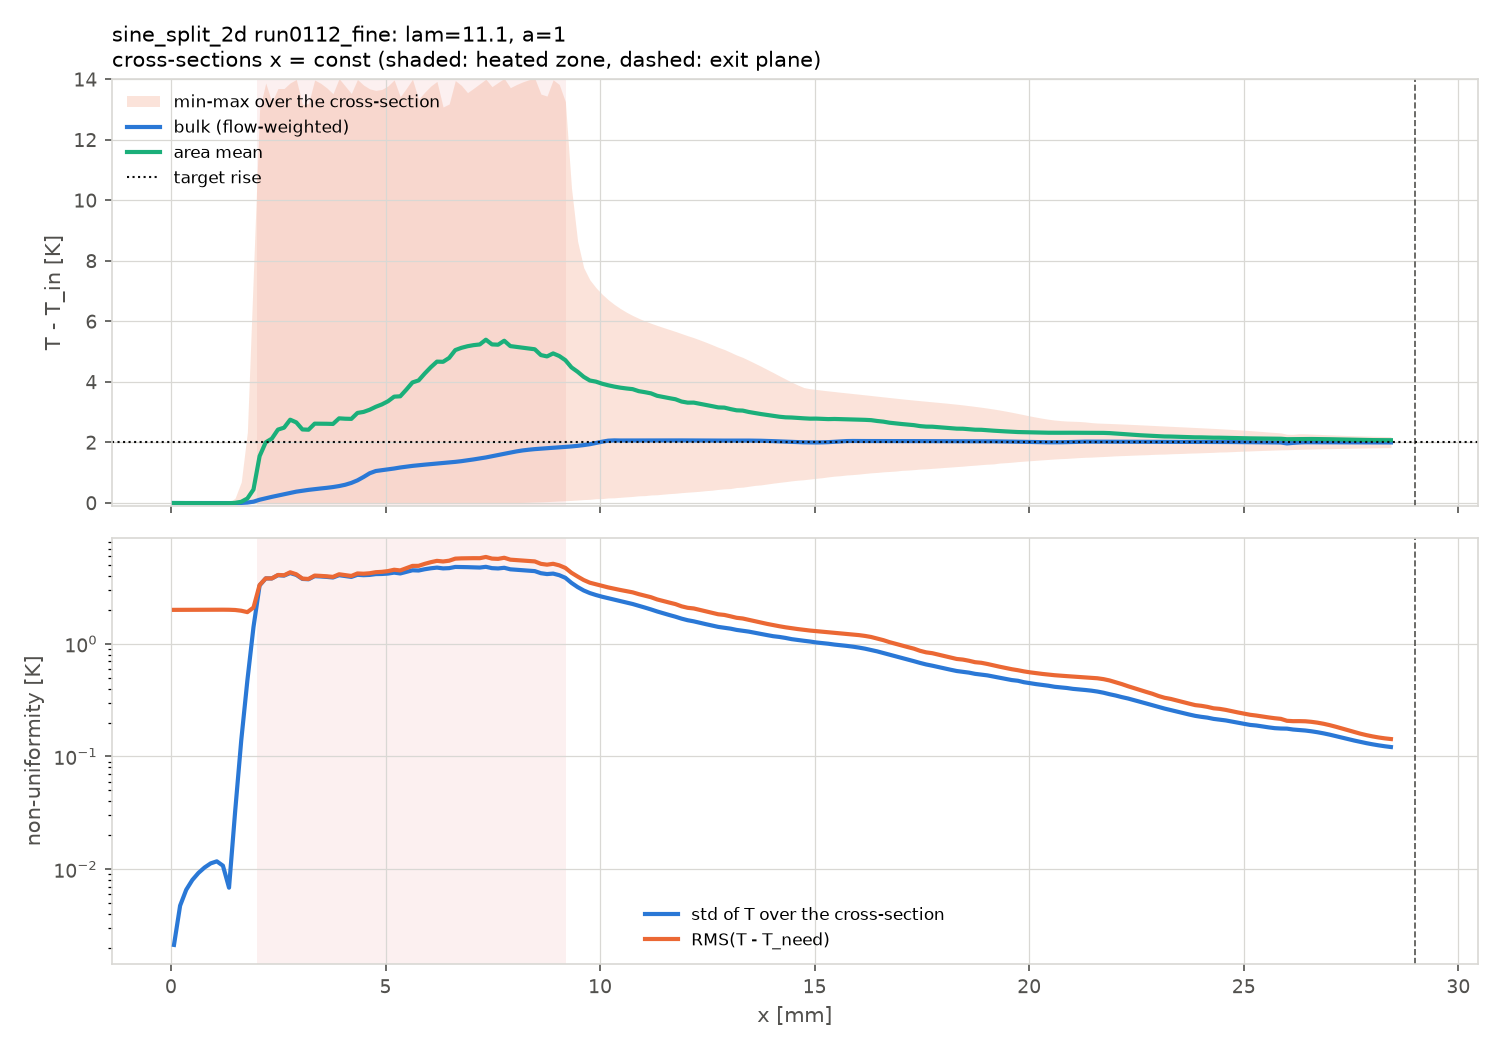
\includegraphics[width=0.8\textwidth,height=0.8\textheight,keepaspectratio]{runs/final_u2d_sine_grid_along_x.png}
\caption{Bulk, mean, min and max temperature along the channel.}
\end{figure}
\begin{figure}[H]\centering
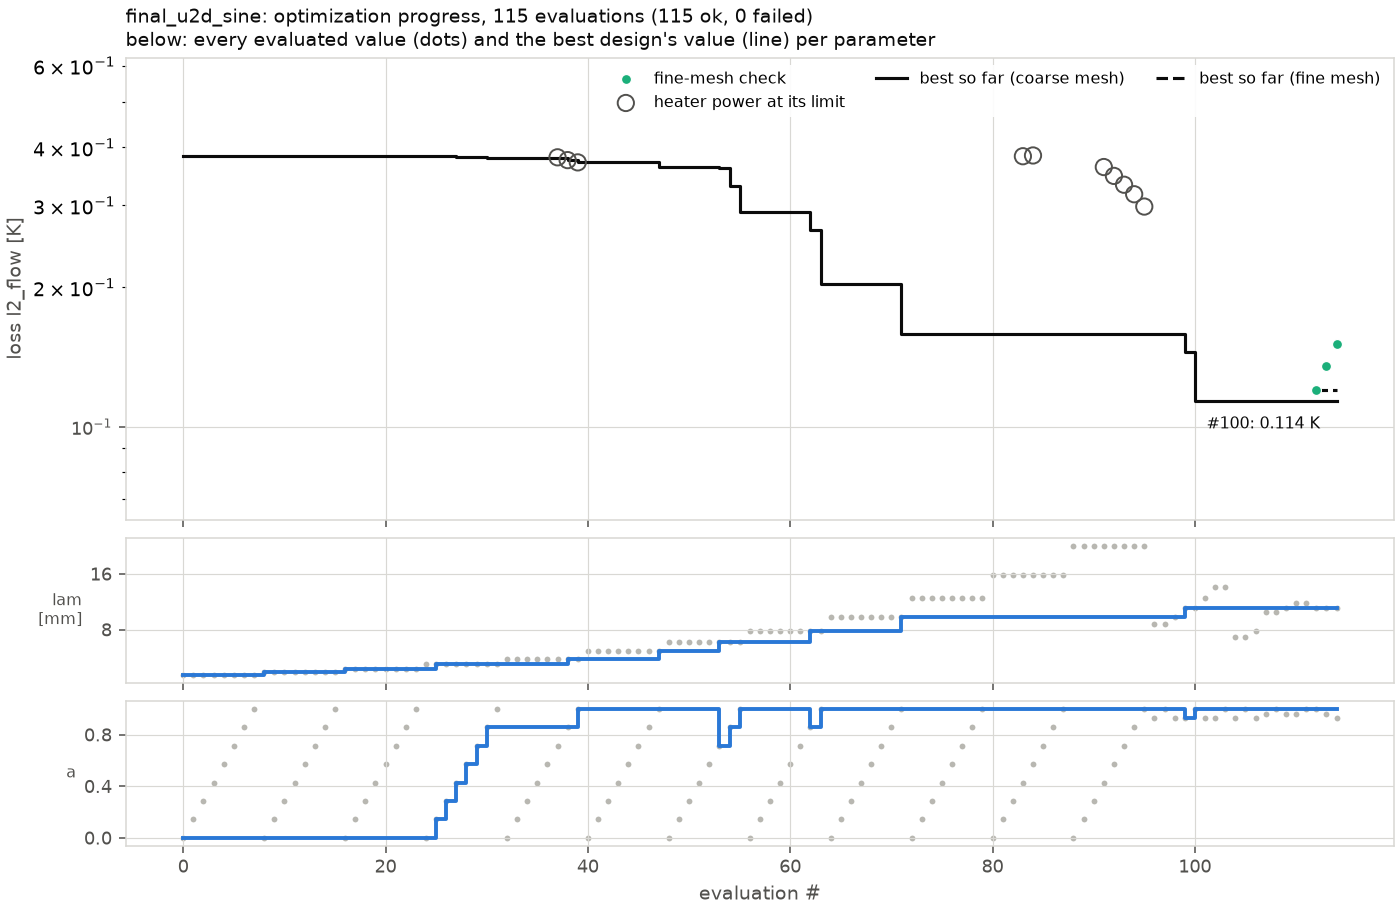
\includegraphics[width=0.85\textwidth]{runs/final_u2d_sine_grid_progress_loss.png}
\caption{Search history: loss of every evaluation, best so far, and the parameters.}
\end{figure}
\clearpage
\subsubsection*{2D serpentine, BO best \#51 ($\lambda$ 8.72, $A$ 3.10, heater 60\,\%): 11.9\mK}
\noindent\texttt{runs/final\_u2d\_serp}\par\medskip
\begin{figure}[H]\centering
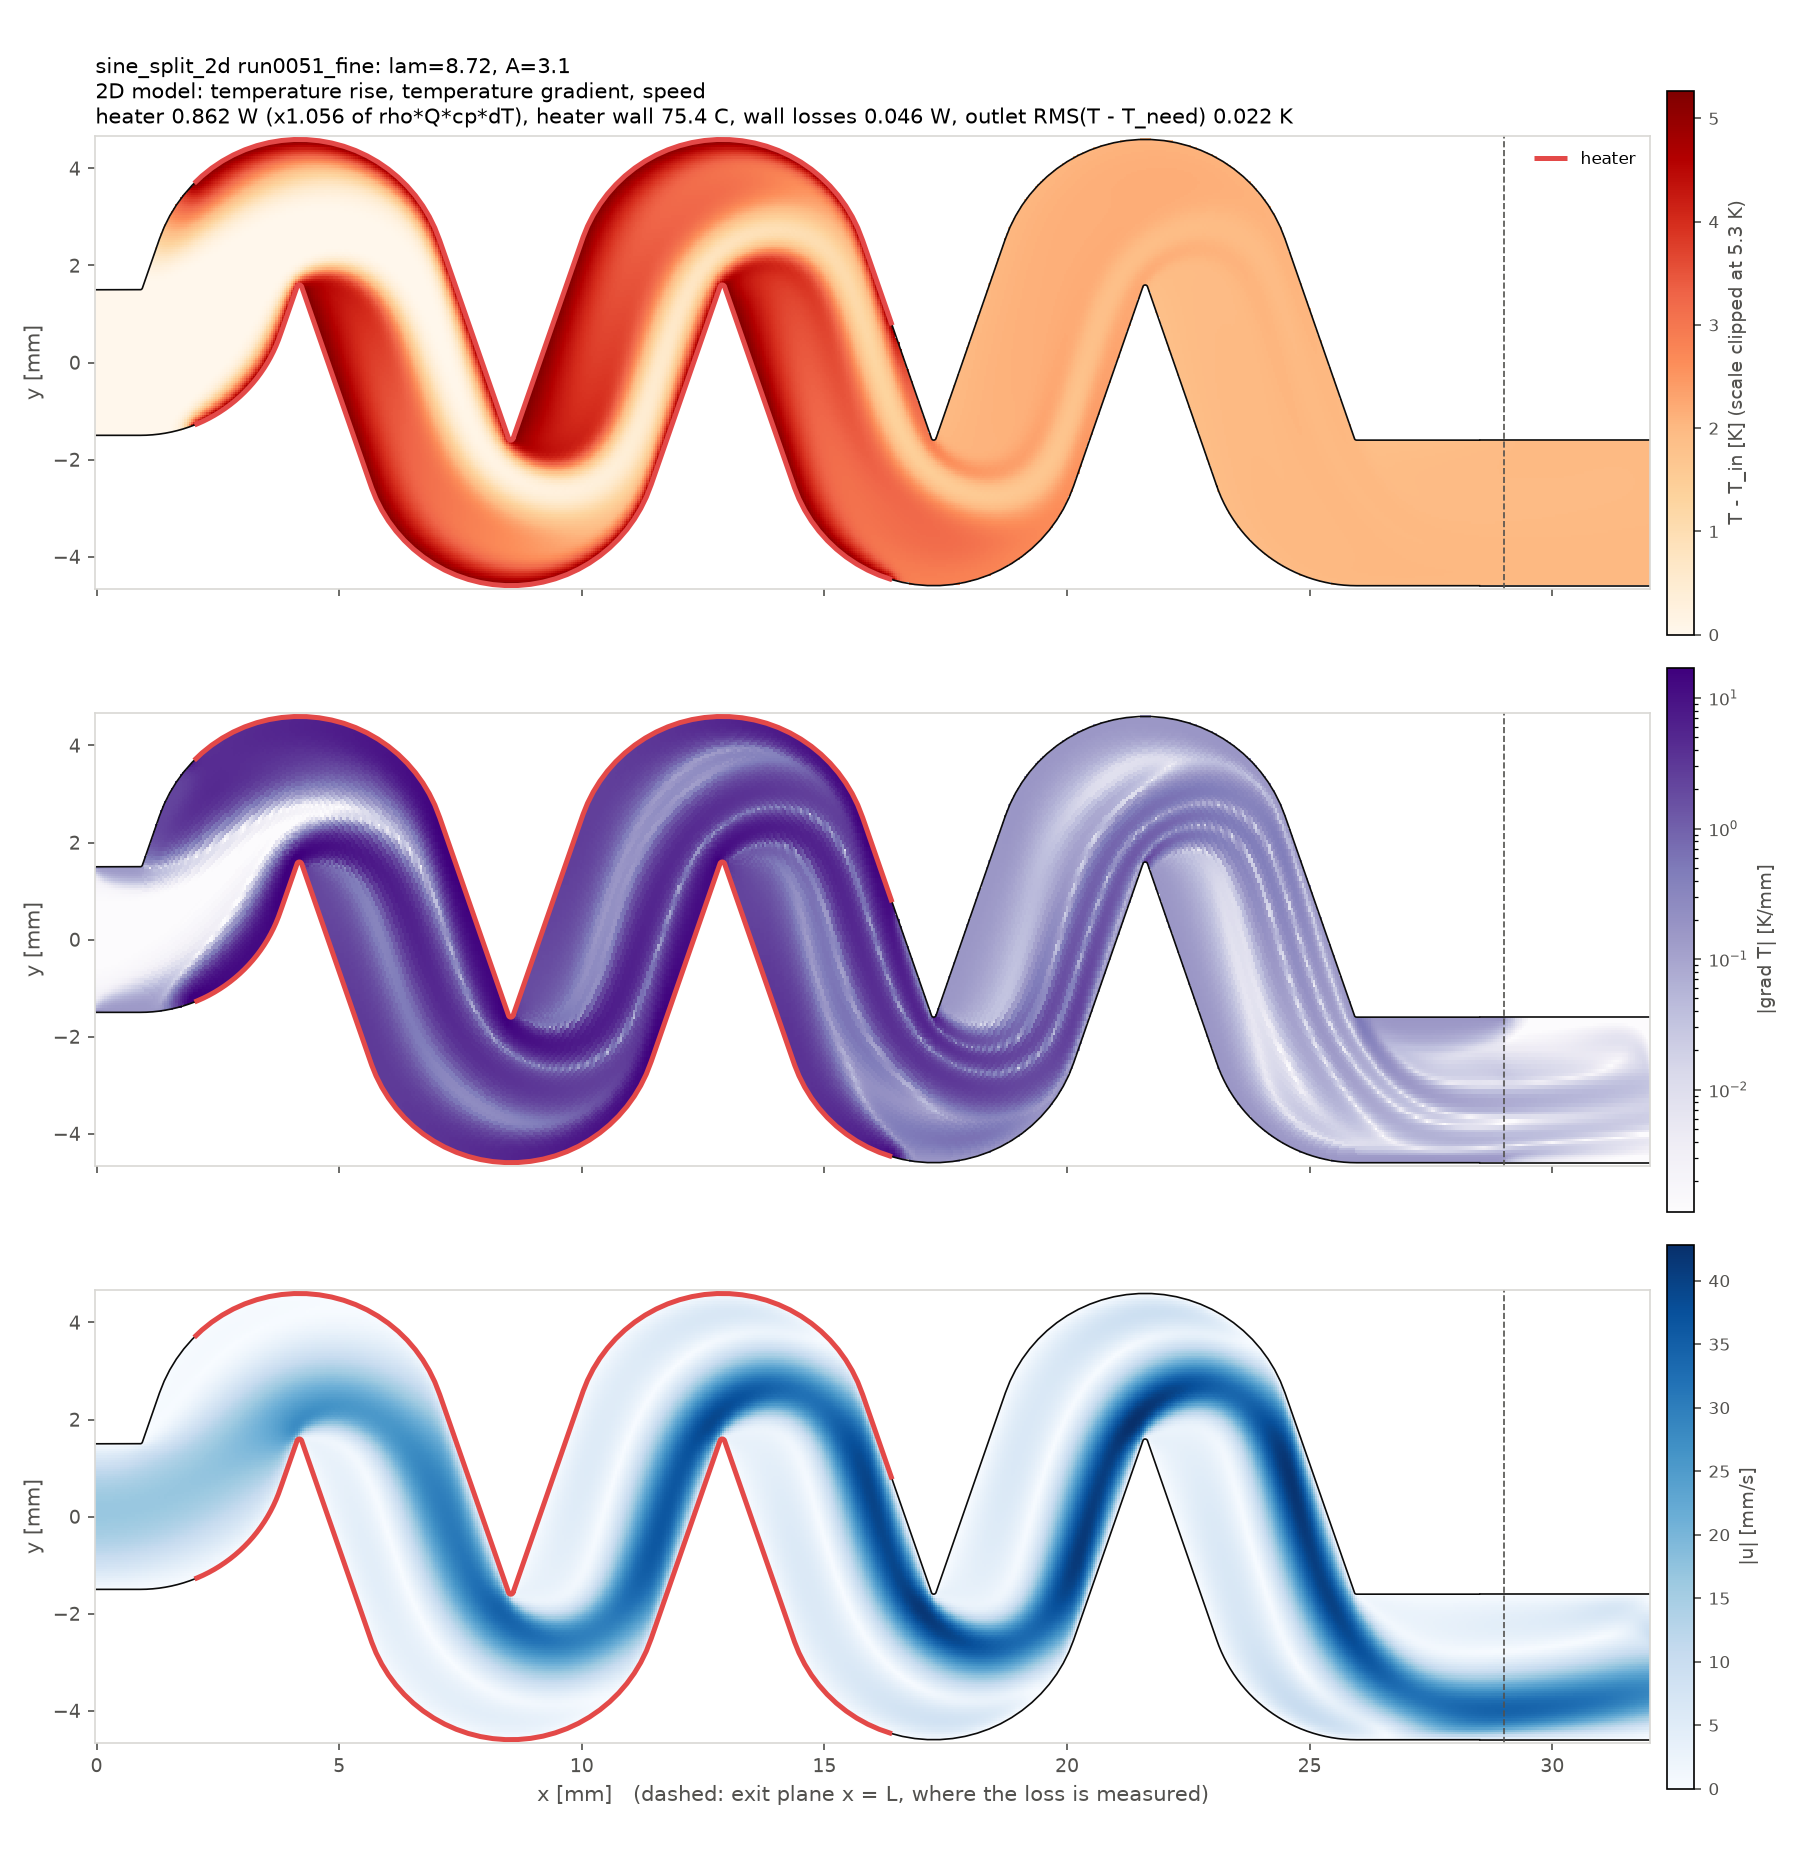
\includegraphics[width=0.95\textwidth,height=0.8\textheight,keepaspectratio]{runs/final_u2d_serp_maps.png}
\caption{Temperature rise, temperature gradient and speed (mid-depth plane in 3D). Red: heated wall. The title's ``outlet RMS'' is the area-weighted $\ell_{2,\mathrm{area}}$.}
\end{figure}
\begin{figure}[H]\centering
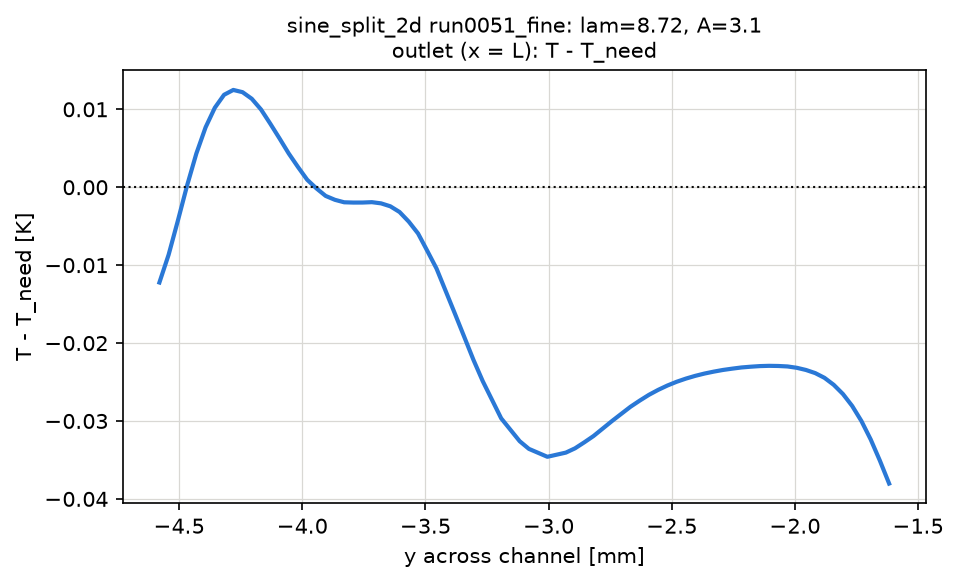
\includegraphics[width=0.75\textwidth,height=0.8\textheight,keepaspectratio]{runs/final_u2d_serp_outlet.png}
\caption{Outlet temperature (and, in 3D, the outlet plane).}
\end{figure}
\begin{figure}[H]\centering
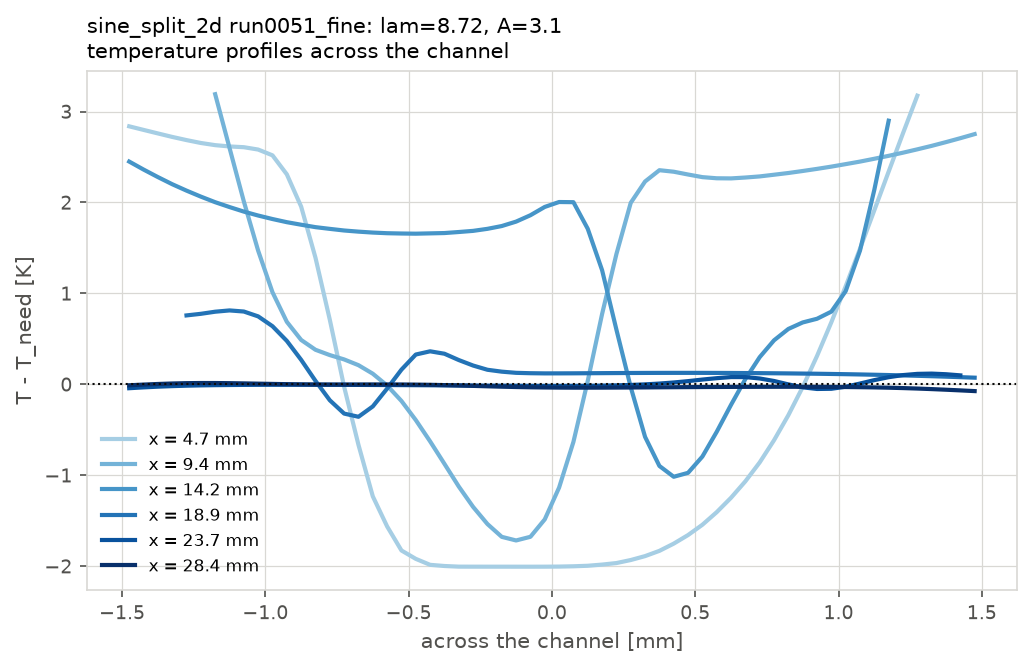
\includegraphics[width=0.62\textwidth,height=0.8\textheight,keepaspectratio]{runs/final_u2d_serp_slices.png}
\caption{Temperature profiles across the channel at several $x$ stations.}
\end{figure}
\begin{figure}[H]\centering
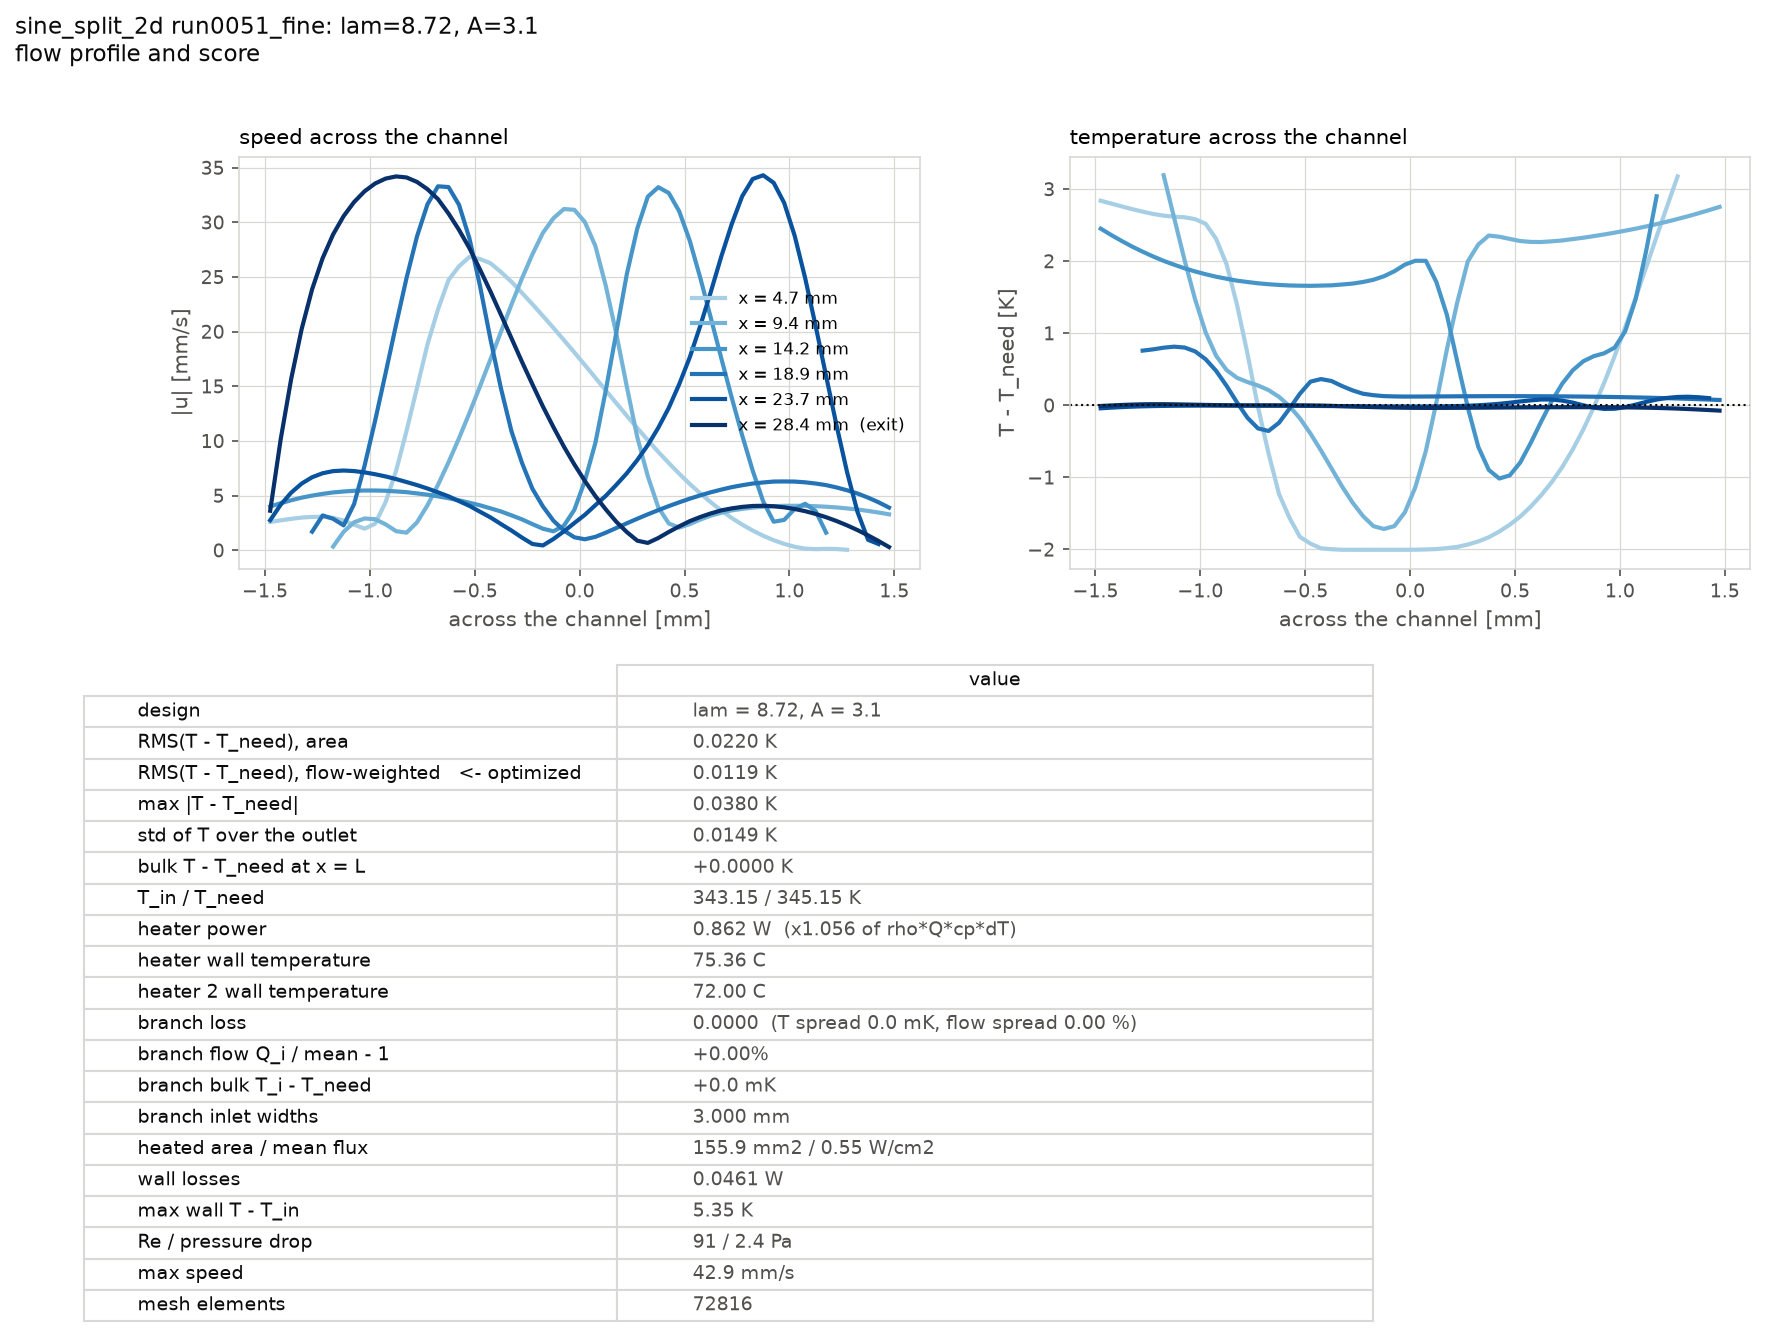
\includegraphics[width=0.8\textwidth,height=0.8\textheight,keepaspectratio]{runs/final_u2d_serp_profile.png}
\caption{Speed and temperature across the channel at several $x$ stations, and the full score table of the design.}
\end{figure}
\begin{figure}[H]\centering
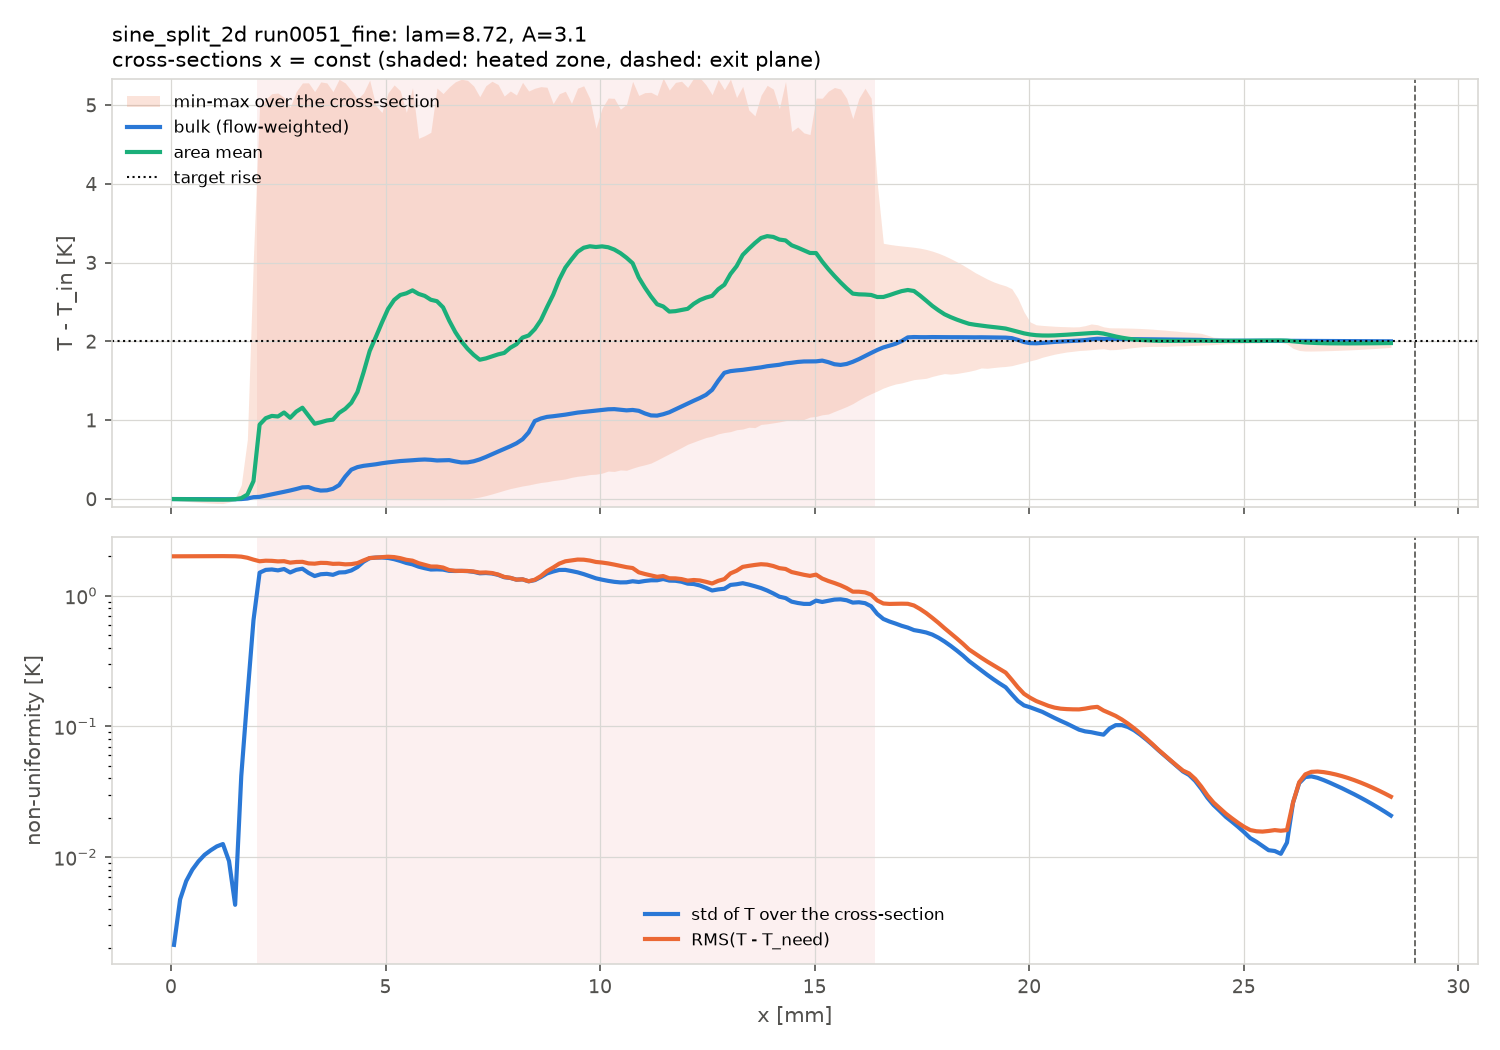
\includegraphics[width=0.8\textwidth,height=0.8\textheight,keepaspectratio]{runs/final_u2d_serp_along_x.png}
\caption{Bulk, mean, min and max temperature along the channel.}
\end{figure}
\begin{figure}[H]\centering
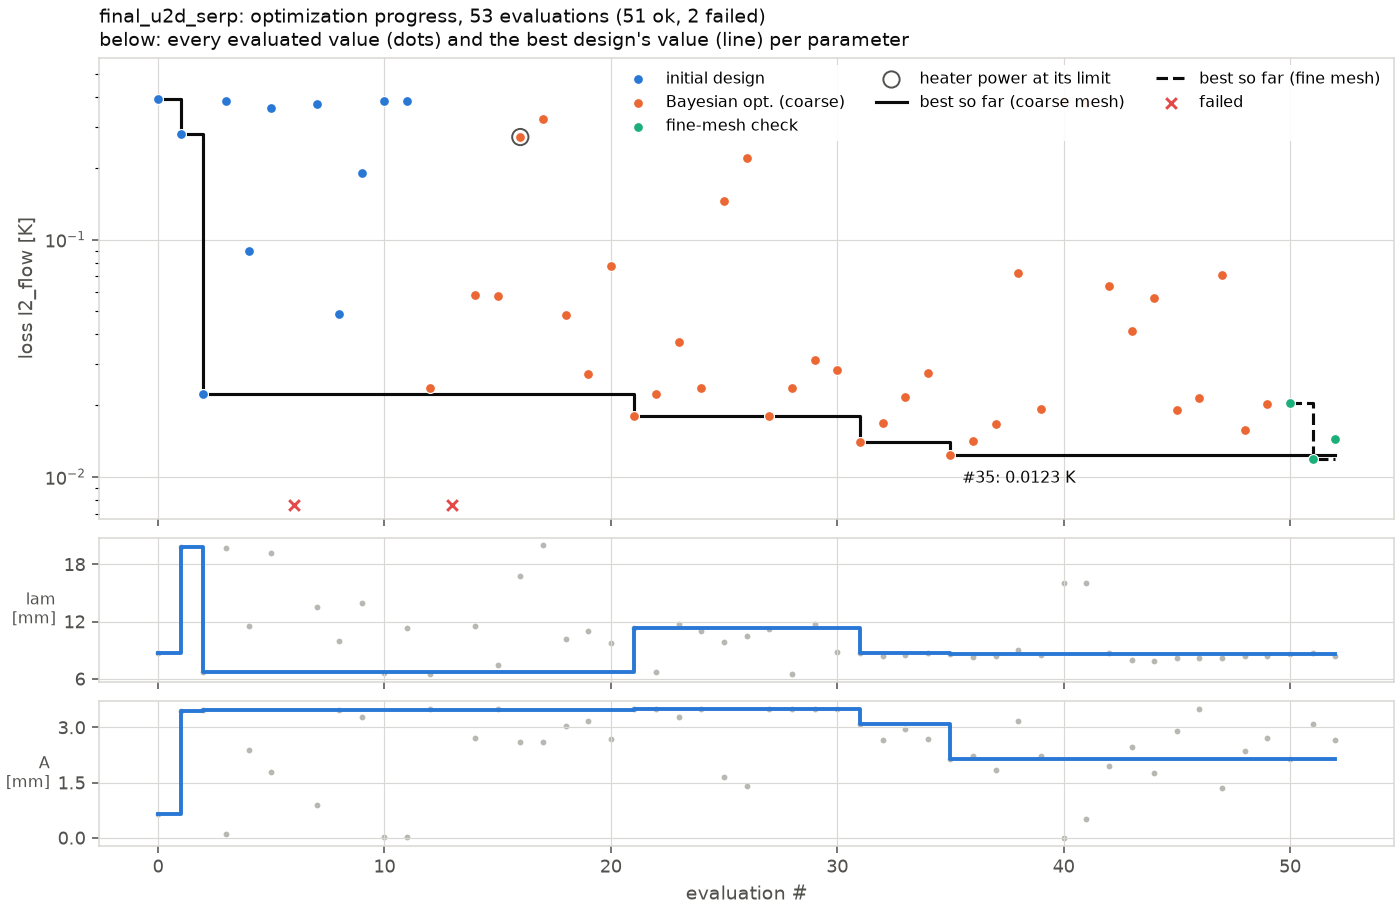
\includegraphics[width=0.85\textwidth]{runs/final_u2d_serp_progress_loss.png}
\caption{Search history: loss of every evaluation, best so far, and the parameters.}
\end{figure}
\clearpage
\subsubsection*{2D serpentine, grid best \#108 ($\lambda$ 8.34, $A$ 2.13, heater 40\,\%): 6.3\mK}
\noindent\texttt{runs/final\_u2d\_serp\_grid}\par\medskip
\begin{figure}[H]\centering
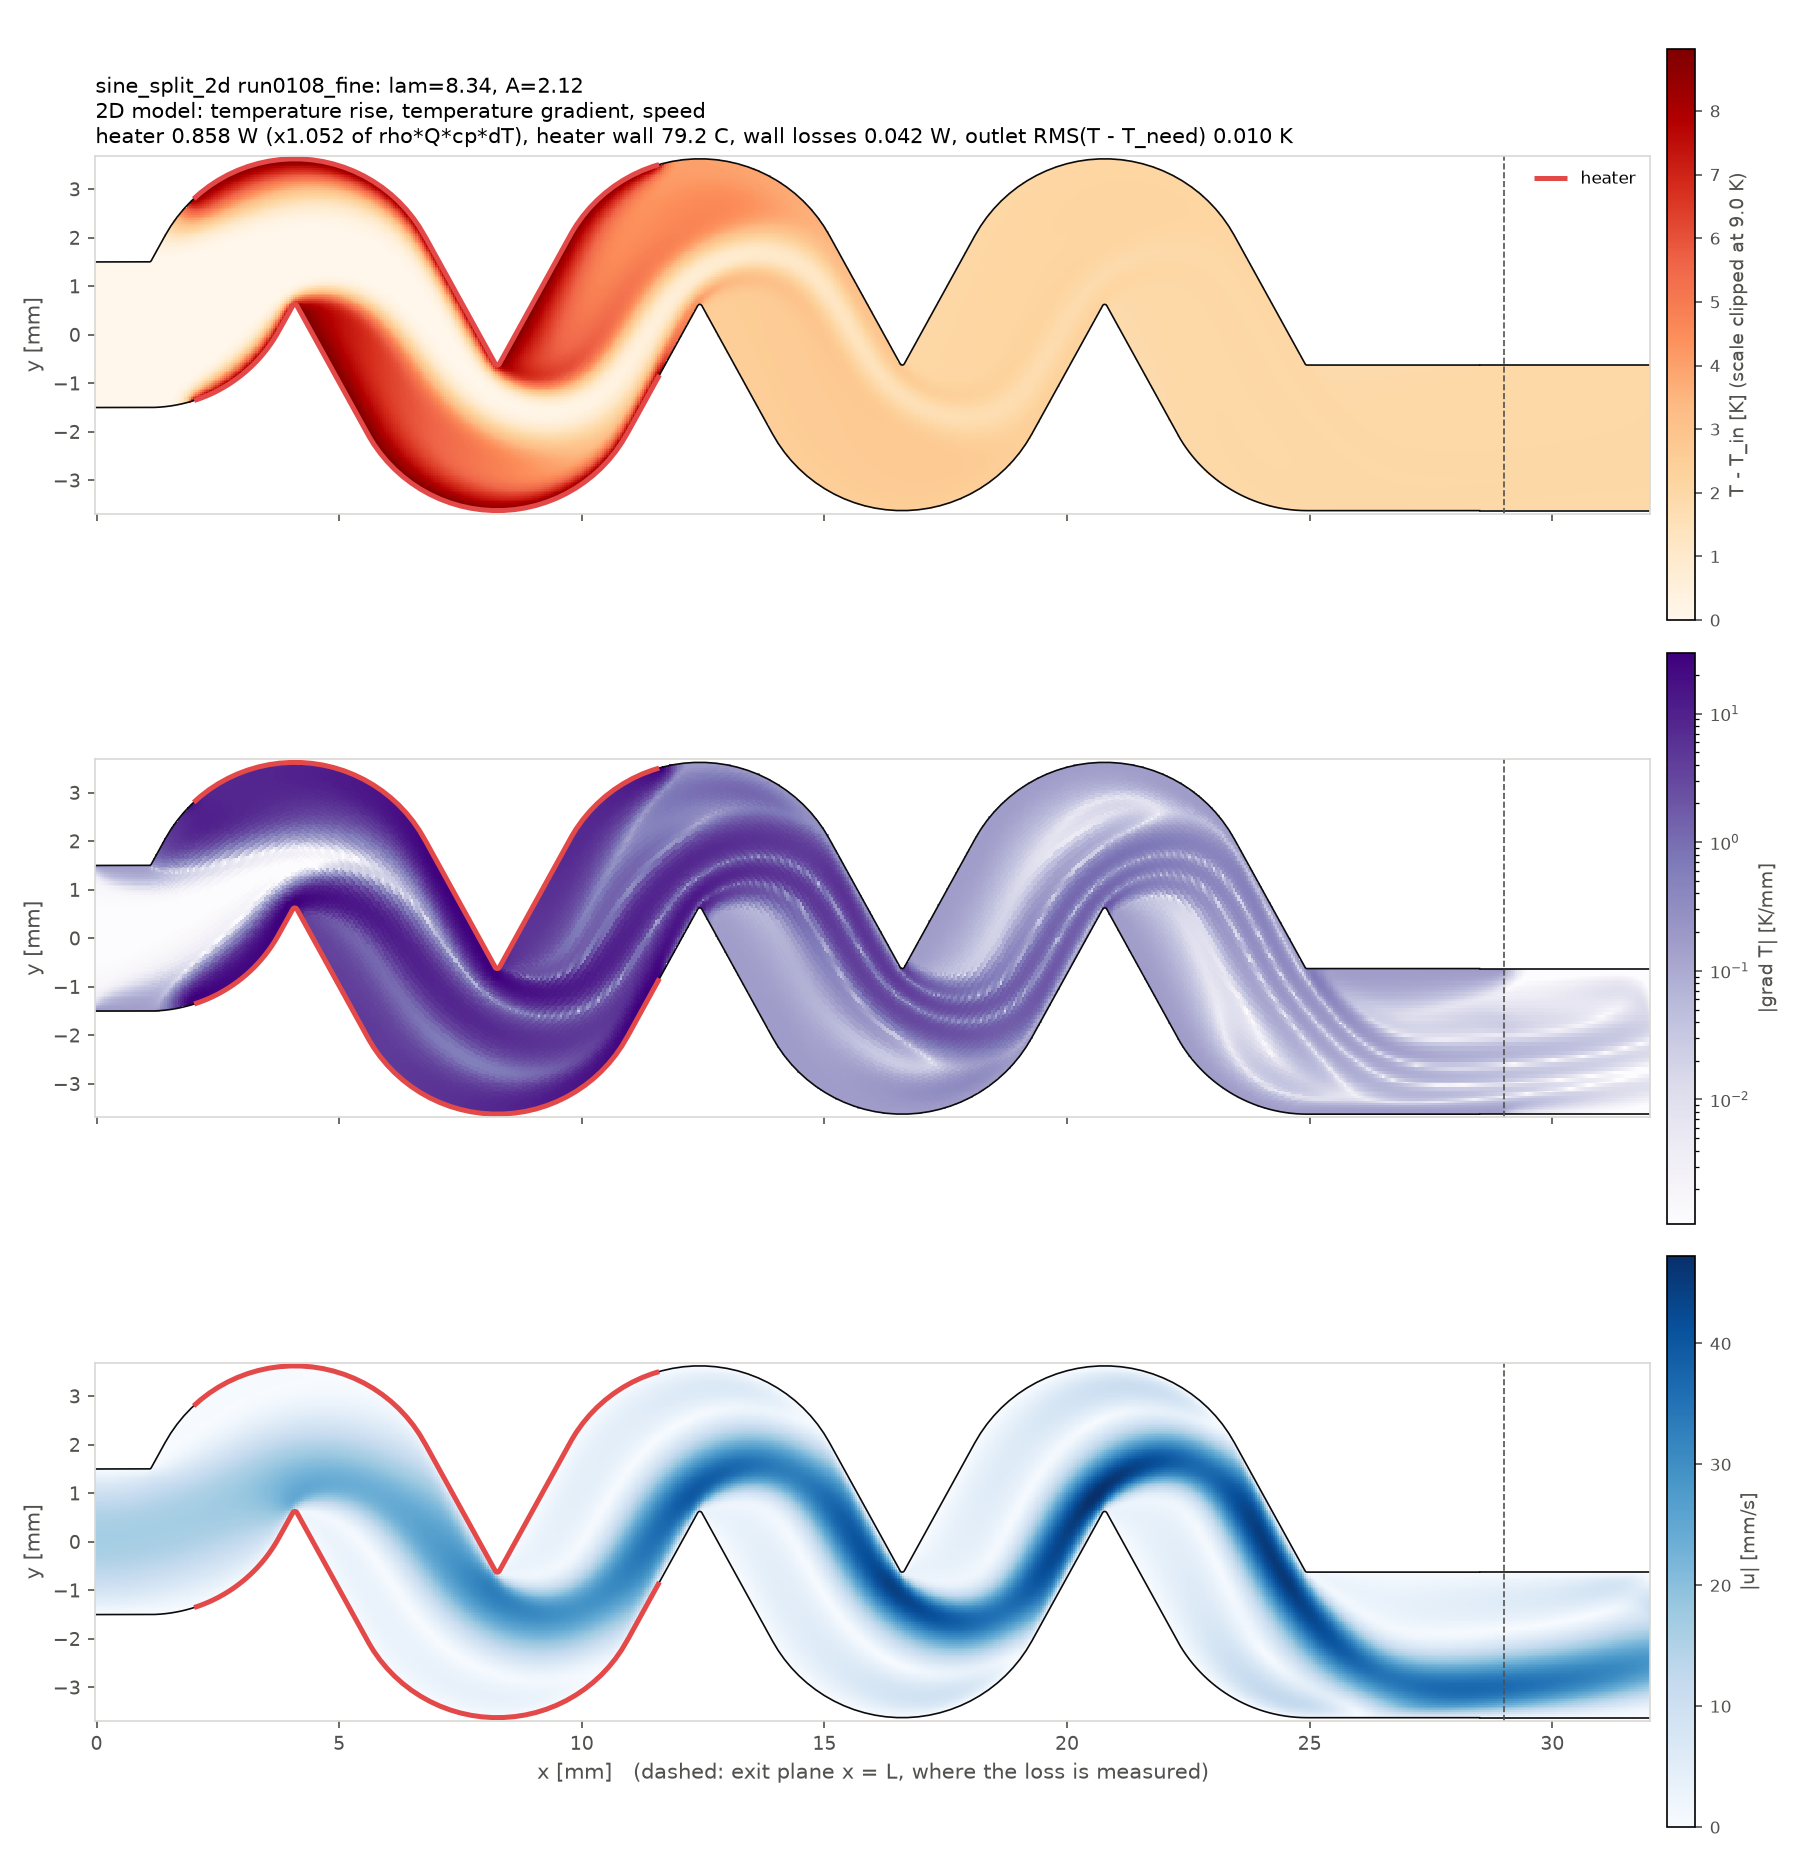
\includegraphics[width=0.95\textwidth,height=0.8\textheight,keepaspectratio]{runs/final_u2d_serp_grid_maps.png}
\caption{Temperature rise, temperature gradient and speed (mid-depth plane in 3D). Red: heated wall. The title's ``outlet RMS'' is the area-weighted $\ell_{2,\mathrm{area}}$.}
\end{figure}
\begin{figure}[H]\centering
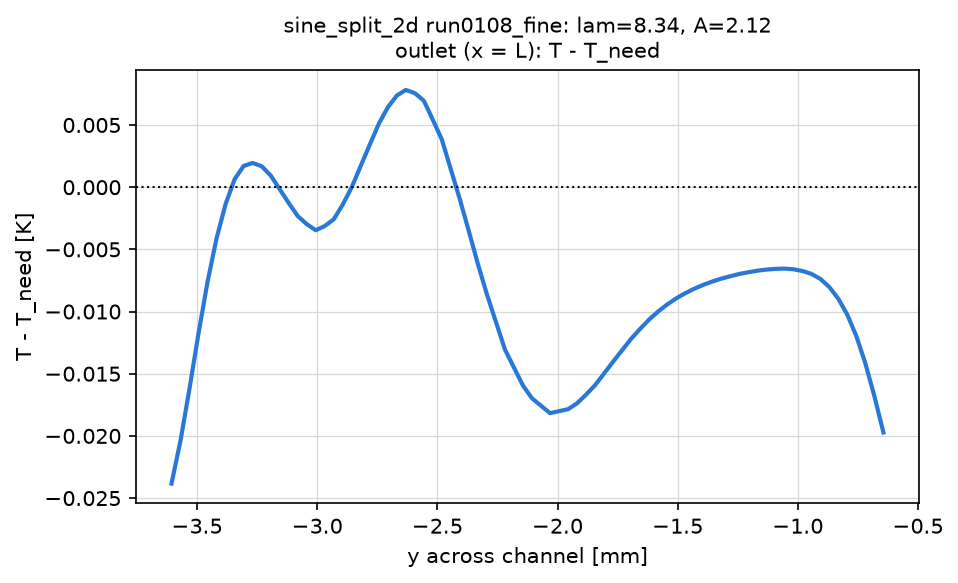
\includegraphics[width=0.75\textwidth,height=0.8\textheight,keepaspectratio]{runs/final_u2d_serp_grid_outlet.png}
\caption{Outlet temperature (and, in 3D, the outlet plane).}
\end{figure}
\begin{figure}[H]\centering
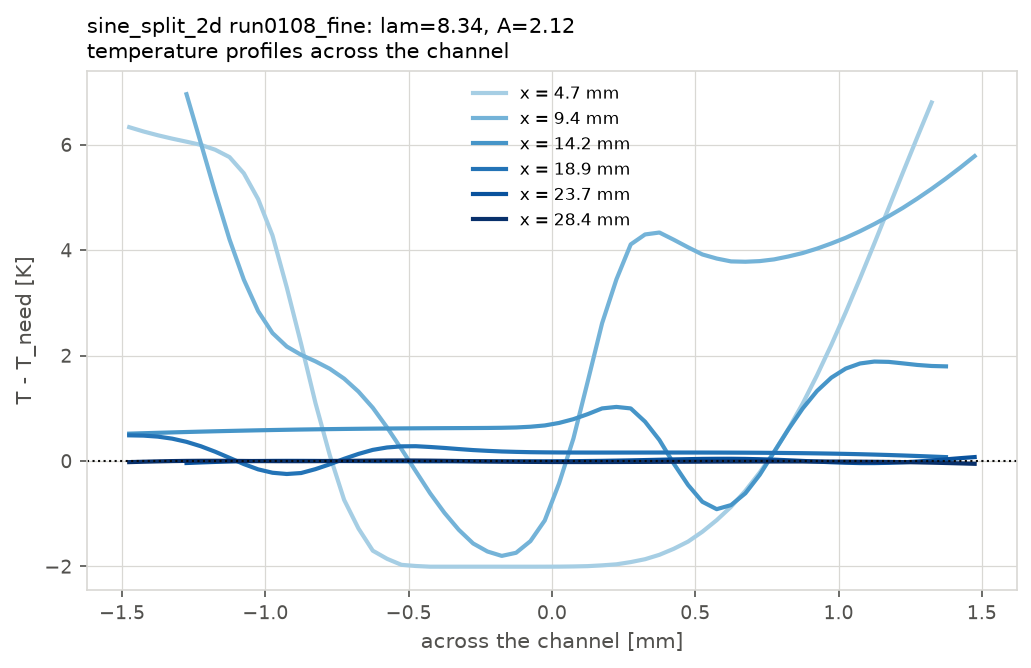
\includegraphics[width=0.62\textwidth,height=0.8\textheight,keepaspectratio]{runs/final_u2d_serp_grid_slices.png}
\caption{Temperature profiles across the channel at several $x$ stations.}
\end{figure}
\begin{figure}[H]\centering
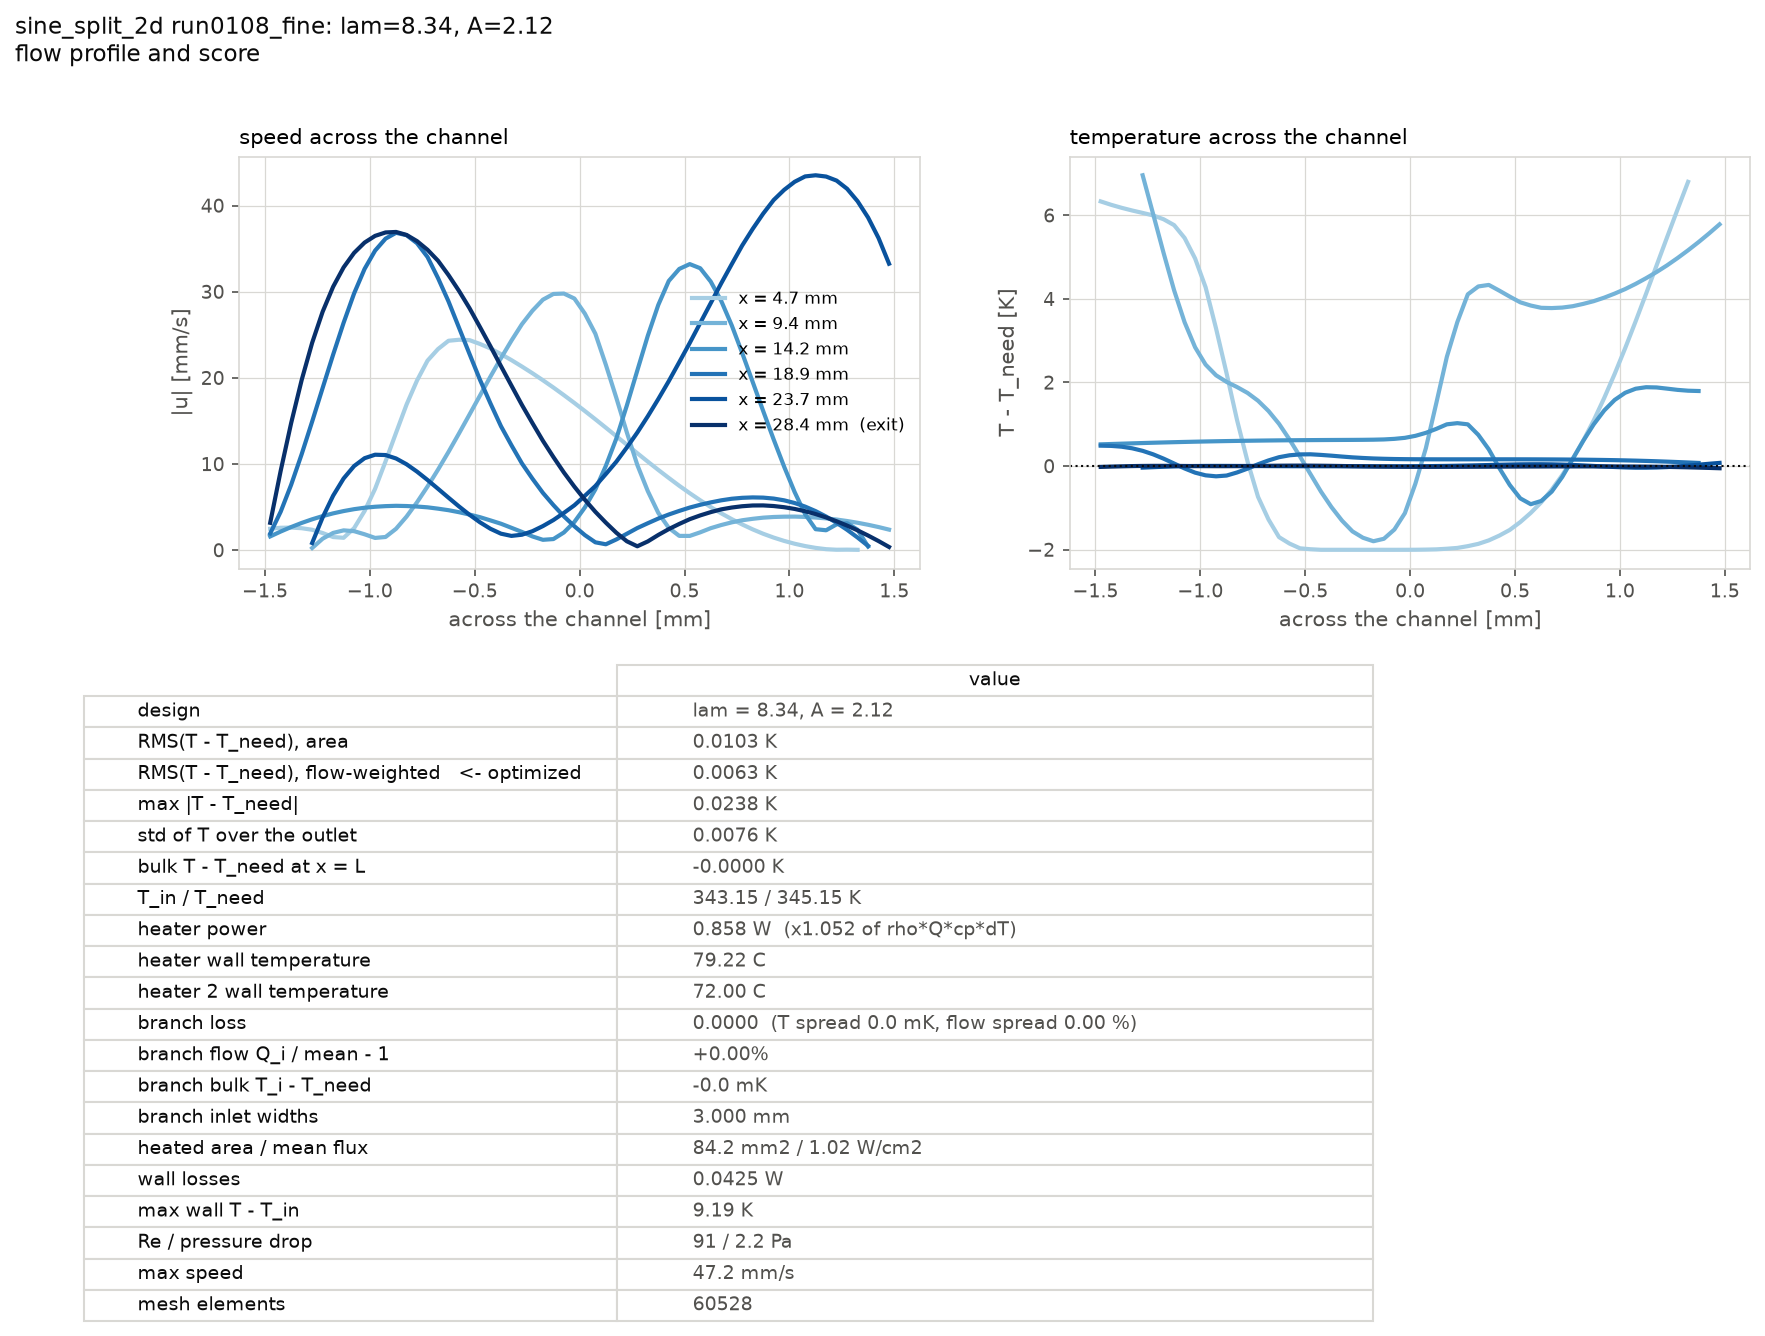
\includegraphics[width=0.8\textwidth,height=0.8\textheight,keepaspectratio]{runs/final_u2d_serp_grid_profile.png}
\caption{Speed and temperature across the channel at several $x$ stations, and the full score table of the design.}
\end{figure}
\begin{figure}[H]\centering
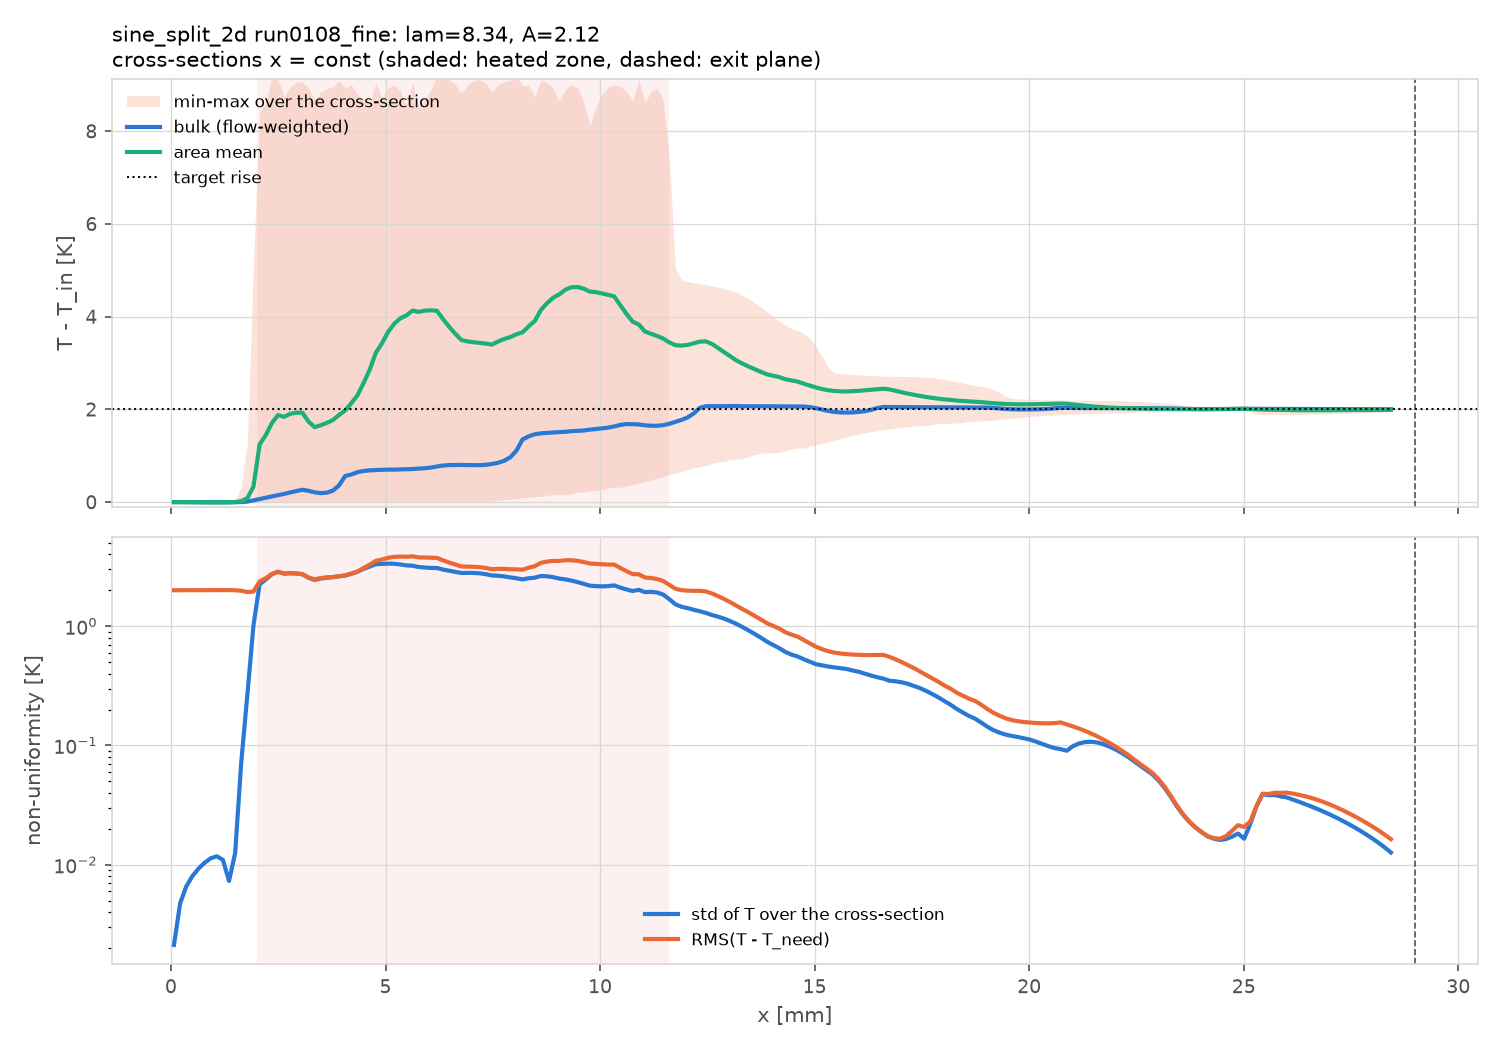
\includegraphics[width=0.8\textwidth,height=0.8\textheight,keepaspectratio]{runs/final_u2d_serp_grid_along_x.png}
\caption{Bulk, mean, min and max temperature along the channel.}
\end{figure}
\begin{figure}[H]\centering
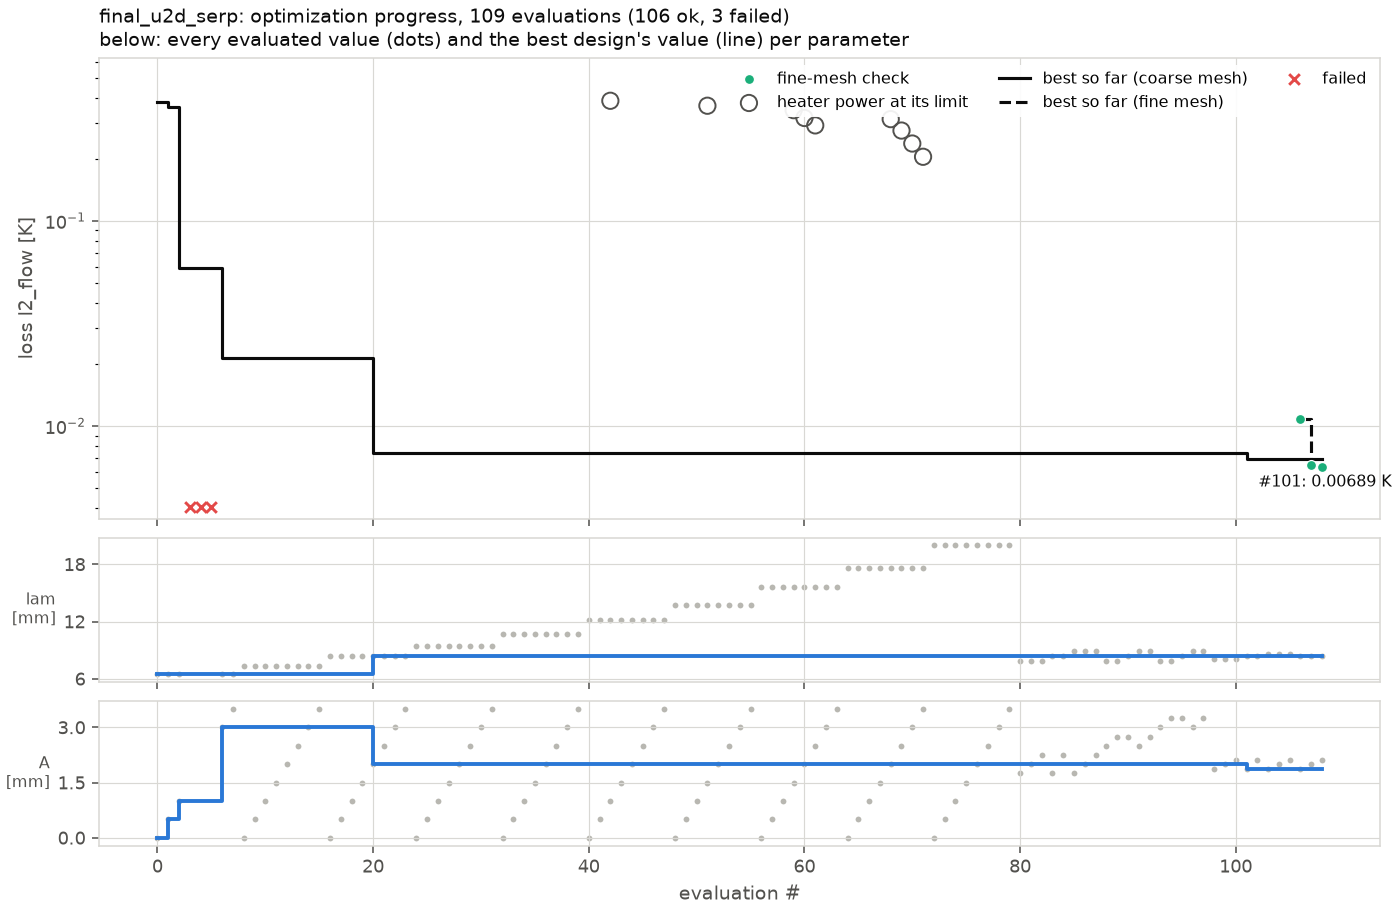
\includegraphics[width=0.85\textwidth]{runs/final_u2d_serp_grid_progress_loss.png}
\caption{Search history: loss of every evaluation, best so far, and the parameters.}
\end{figure}
\subsection{One outlet, 3D (depth 3\,mm)}
\clearpage
\subsubsection*{3D straight reference, fully heated (heater on all four walls, 24\mm)}
\noindent\texttt{runs/final\_u3d\_straight\_ref\_single}\par\medskip
\begin{figure}[H]\centering
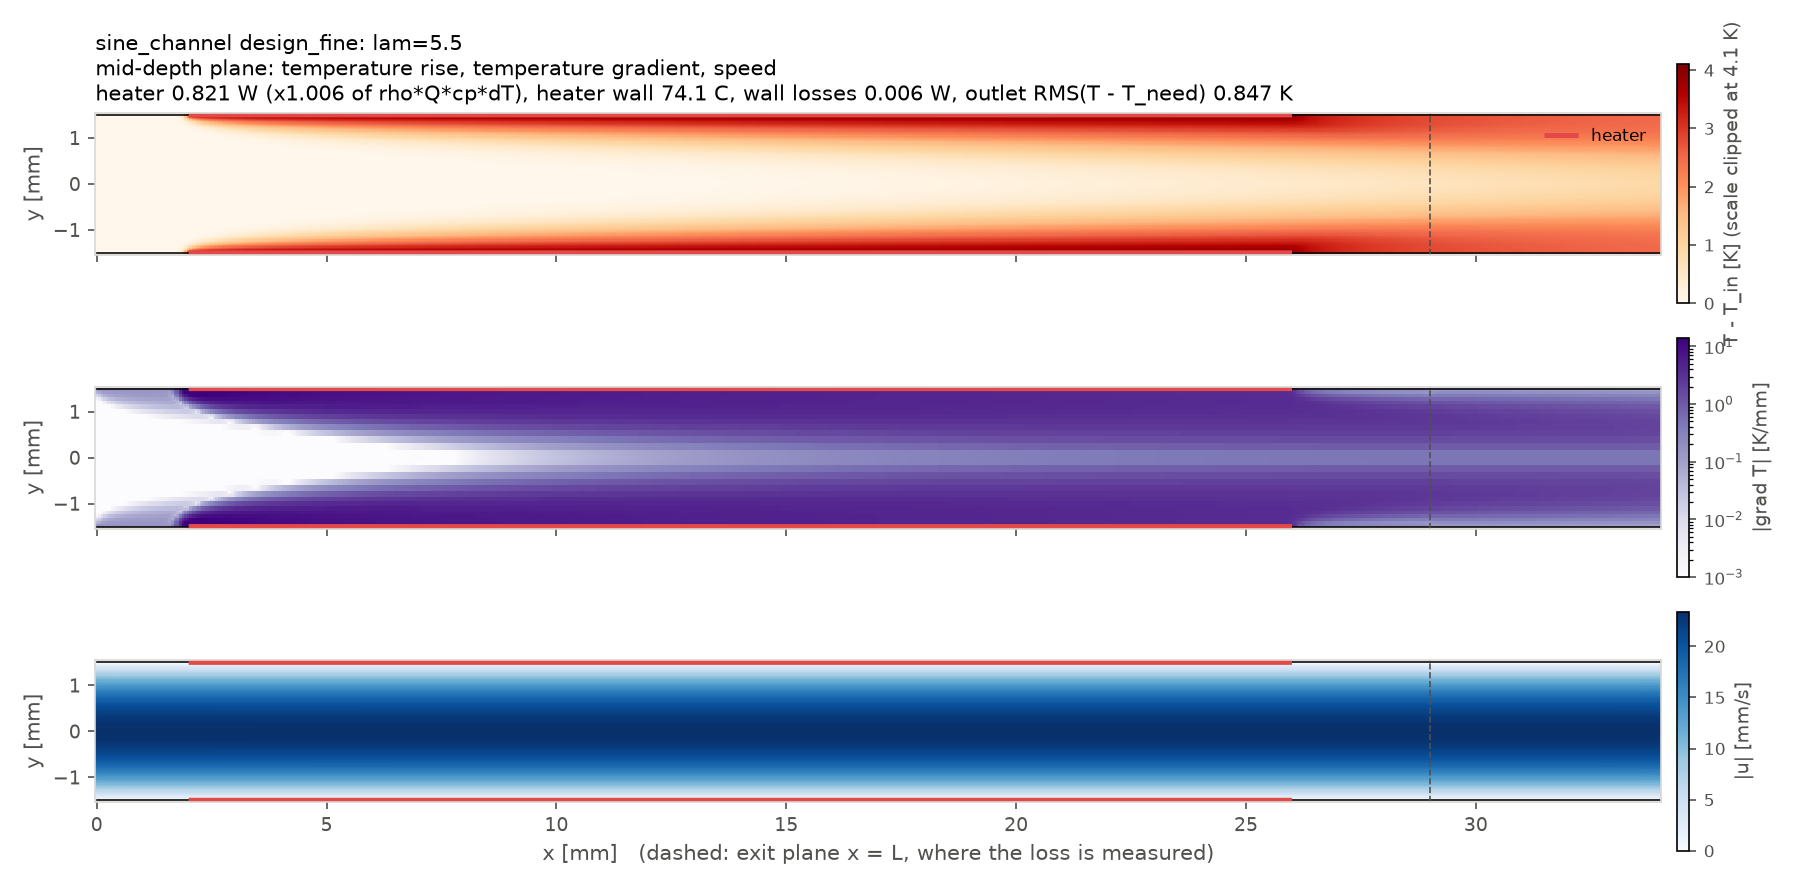
\includegraphics[width=0.95\textwidth,height=0.8\textheight,keepaspectratio]{runs/final_u3d_straight_ref_single_maps.png}
\caption{Temperature rise, temperature gradient and speed (mid-depth plane in 3D). Red: heated wall. The title's ``outlet RMS'' is the area-weighted $\ell_{2,\mathrm{area}}$.}
\end{figure}
\begin{figure}[H]\centering
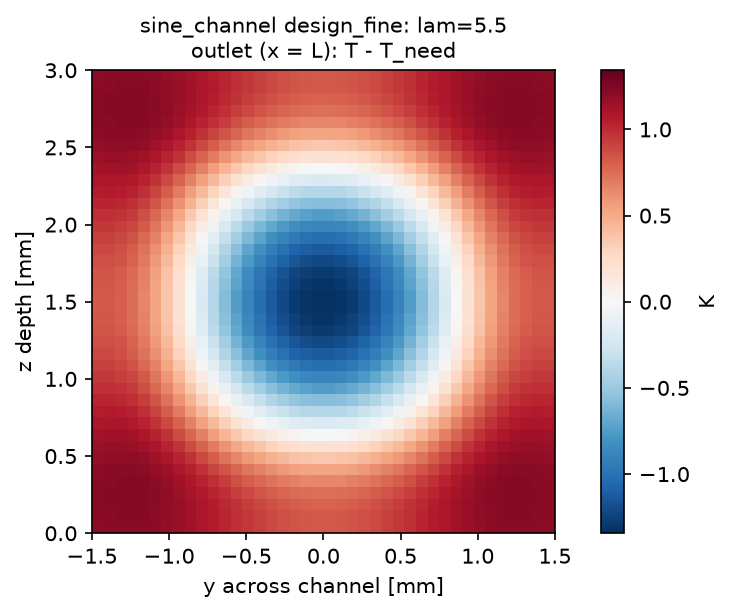
\includegraphics[width=0.75\textwidth,height=0.8\textheight,keepaspectratio]{runs/final_u3d_straight_ref_single_outlet.png}
\caption{Outlet temperature (and, in 3D, the outlet plane).}
\end{figure}
\begin{figure}[H]\centering
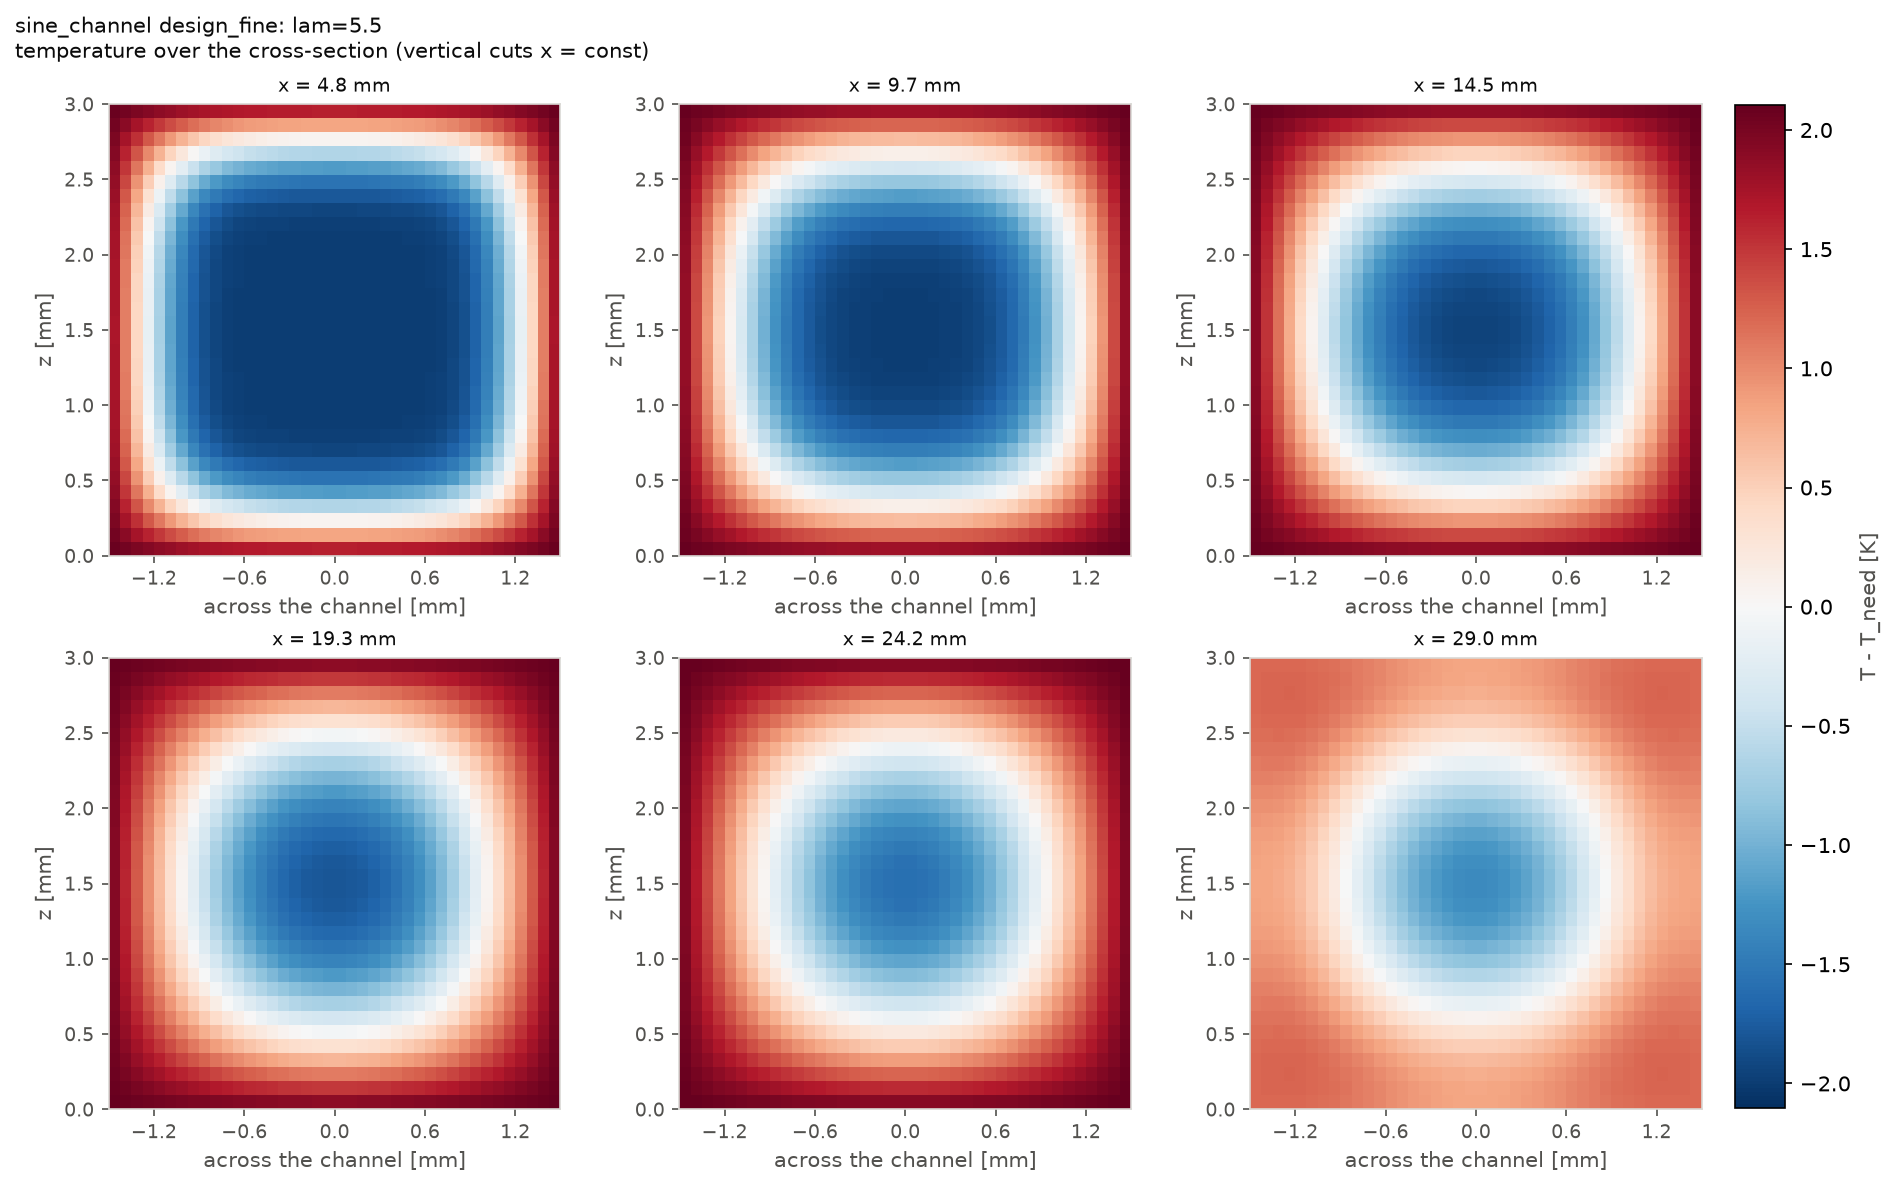
\includegraphics[width=0.62\textwidth,height=0.8\textheight,keepaspectratio]{runs/final_u3d_straight_ref_single_slices.png}
\caption{Temperature profiles across the channel at several $x$ stations.}
\end{figure}
\begin{figure}[H]\centering
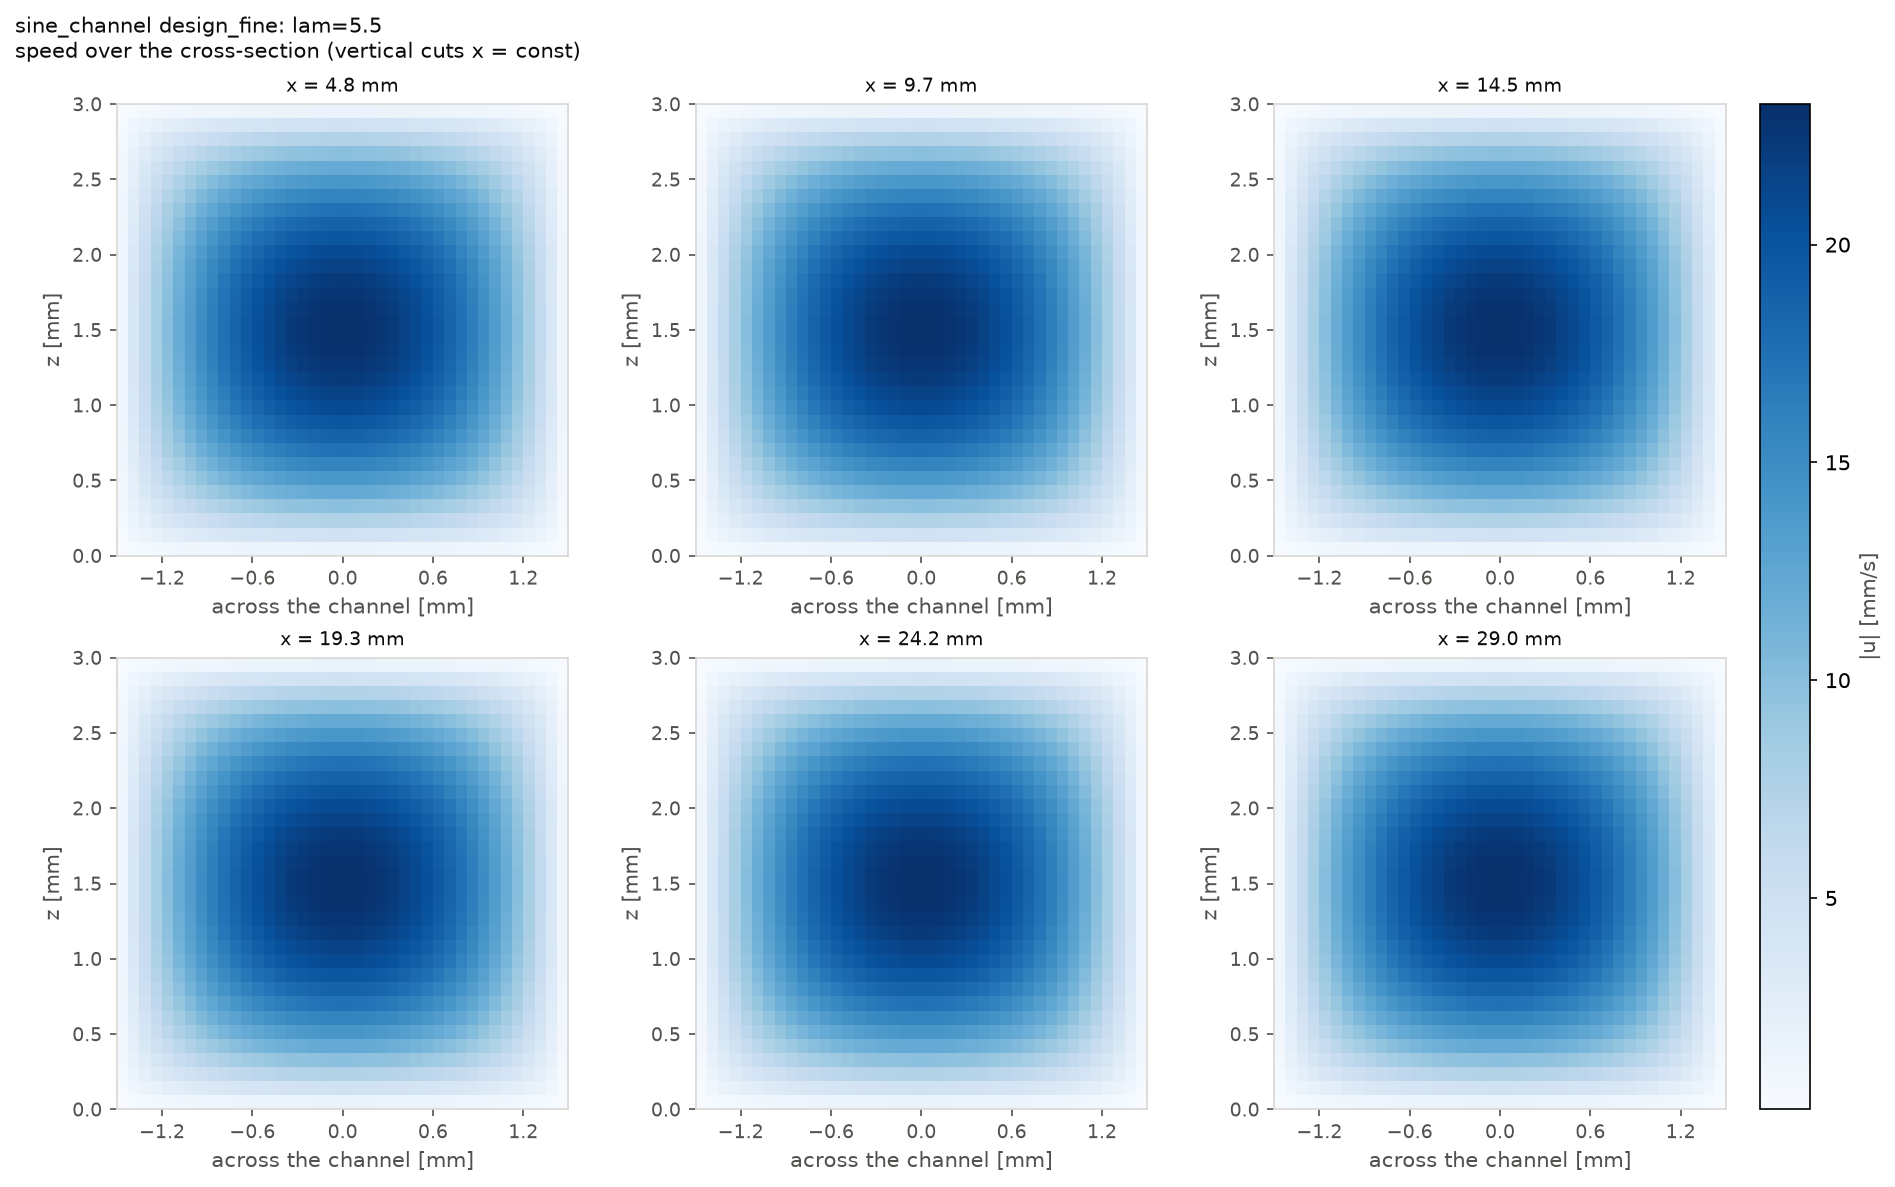
\includegraphics[width=0.85\textwidth,height=0.8\textheight,keepaspectratio]{runs/final_u3d_straight_ref_single_slices_u.png}
\caption{Velocity on cross-sections (3D).}
\end{figure}
\begin{figure}[H]\centering
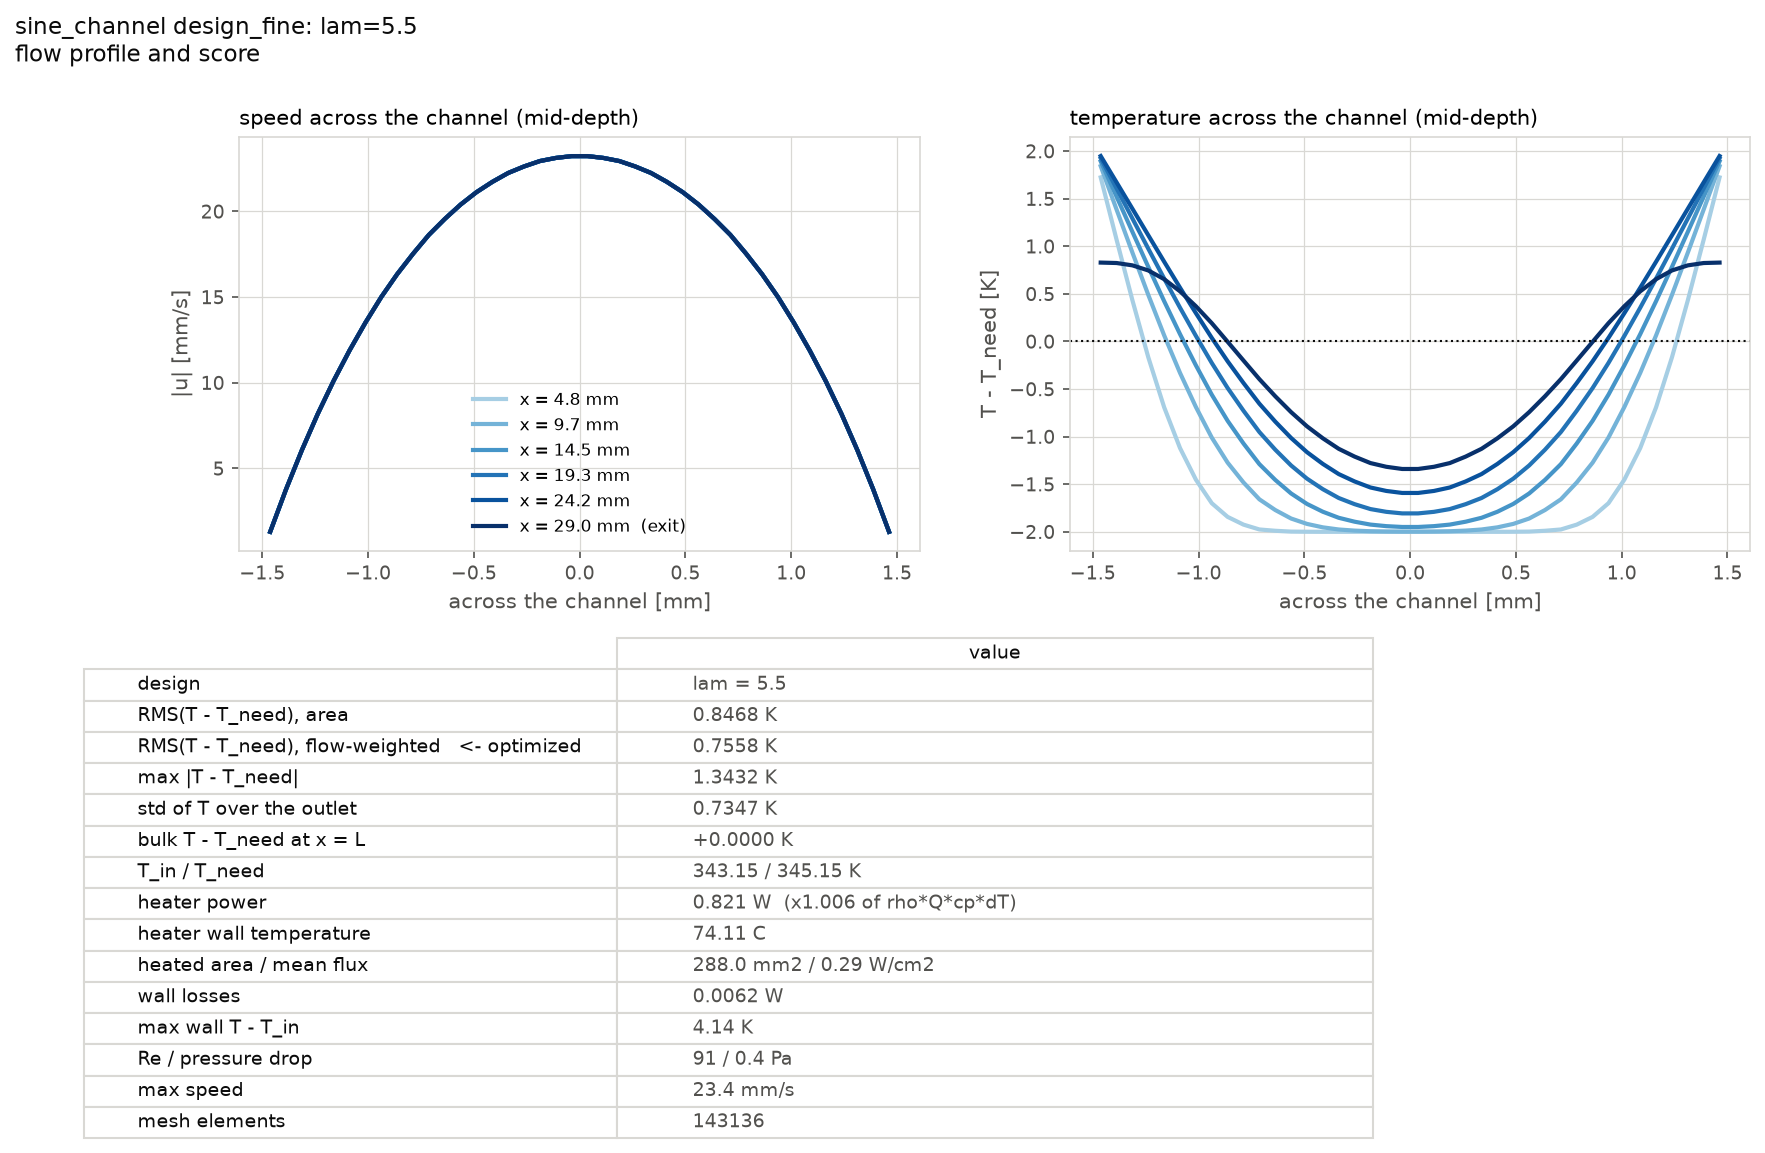
\includegraphics[width=0.8\textwidth,height=0.8\textheight,keepaspectratio]{runs/final_u3d_straight_ref_single_profile.png}
\caption{Speed and temperature across the channel at several $x$ stations, and the full score table of the design.}
\end{figure}
\begin{figure}[H]\centering
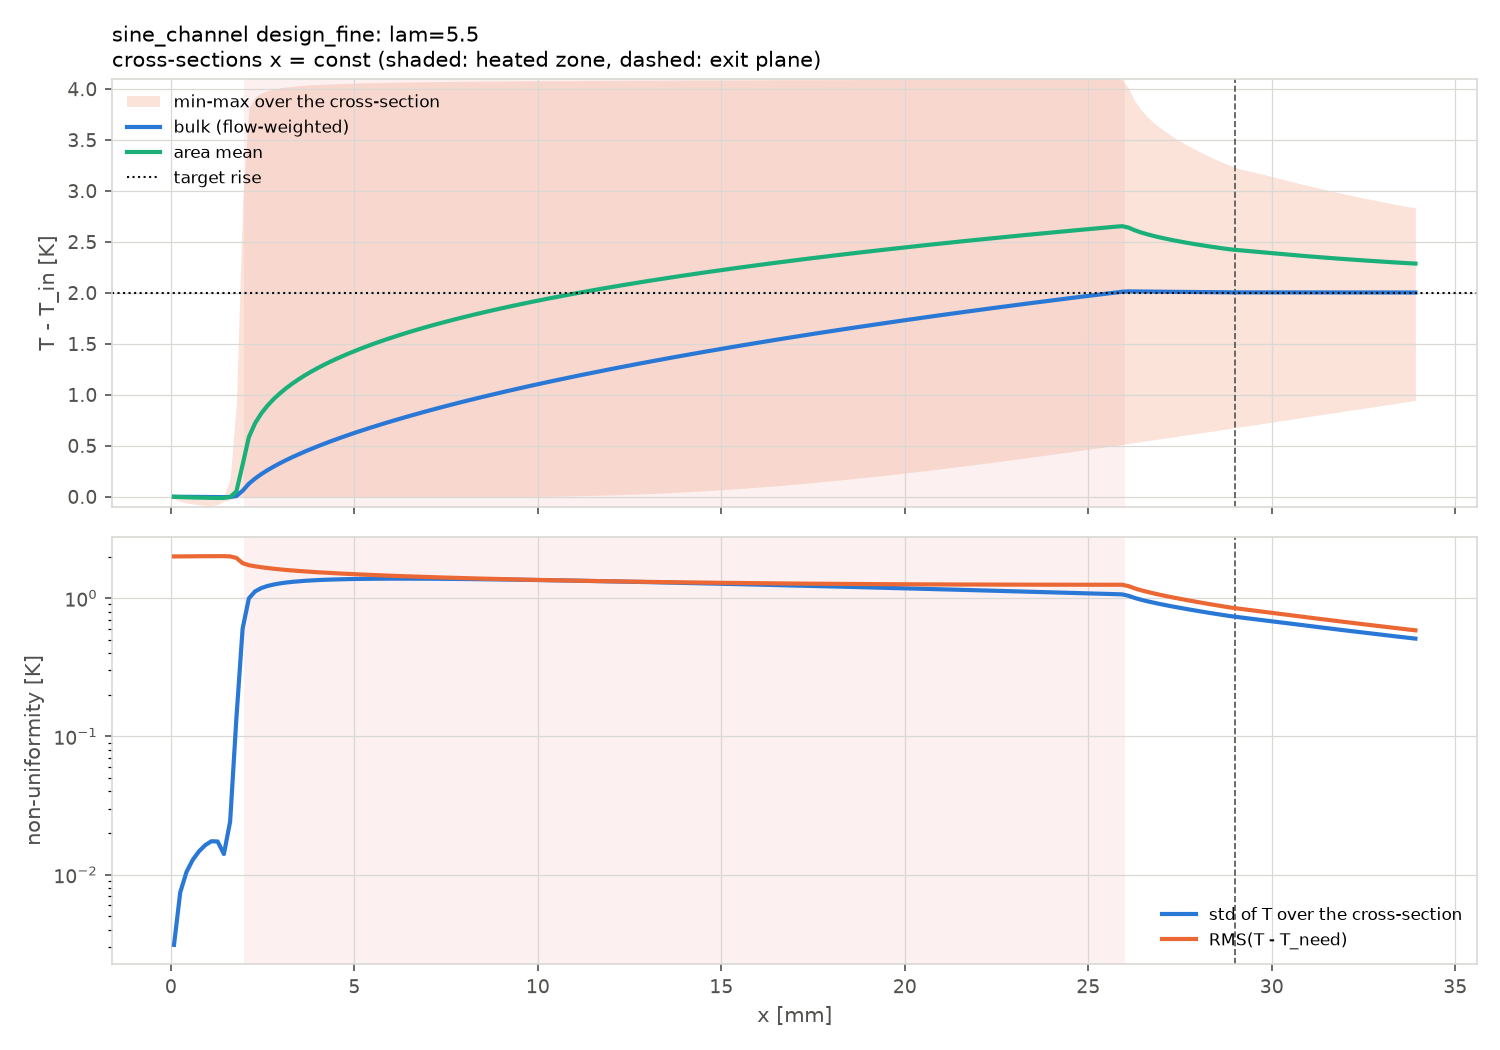
\includegraphics[width=0.8\textwidth,height=0.8\textheight,keepaspectratio]{runs/final_u3d_straight_ref_single_along_x.png}
\caption{Bulk, mean, min and max temperature along the channel.}
\end{figure}
\clearpage
\subsubsection*{3D straight reference, best heater window (1.2\mm{} at the start): 378\mK}
\noindent\texttt{runs/final\_u3d\_straight\_ref}\par\medskip
\begin{figure}[H]\centering
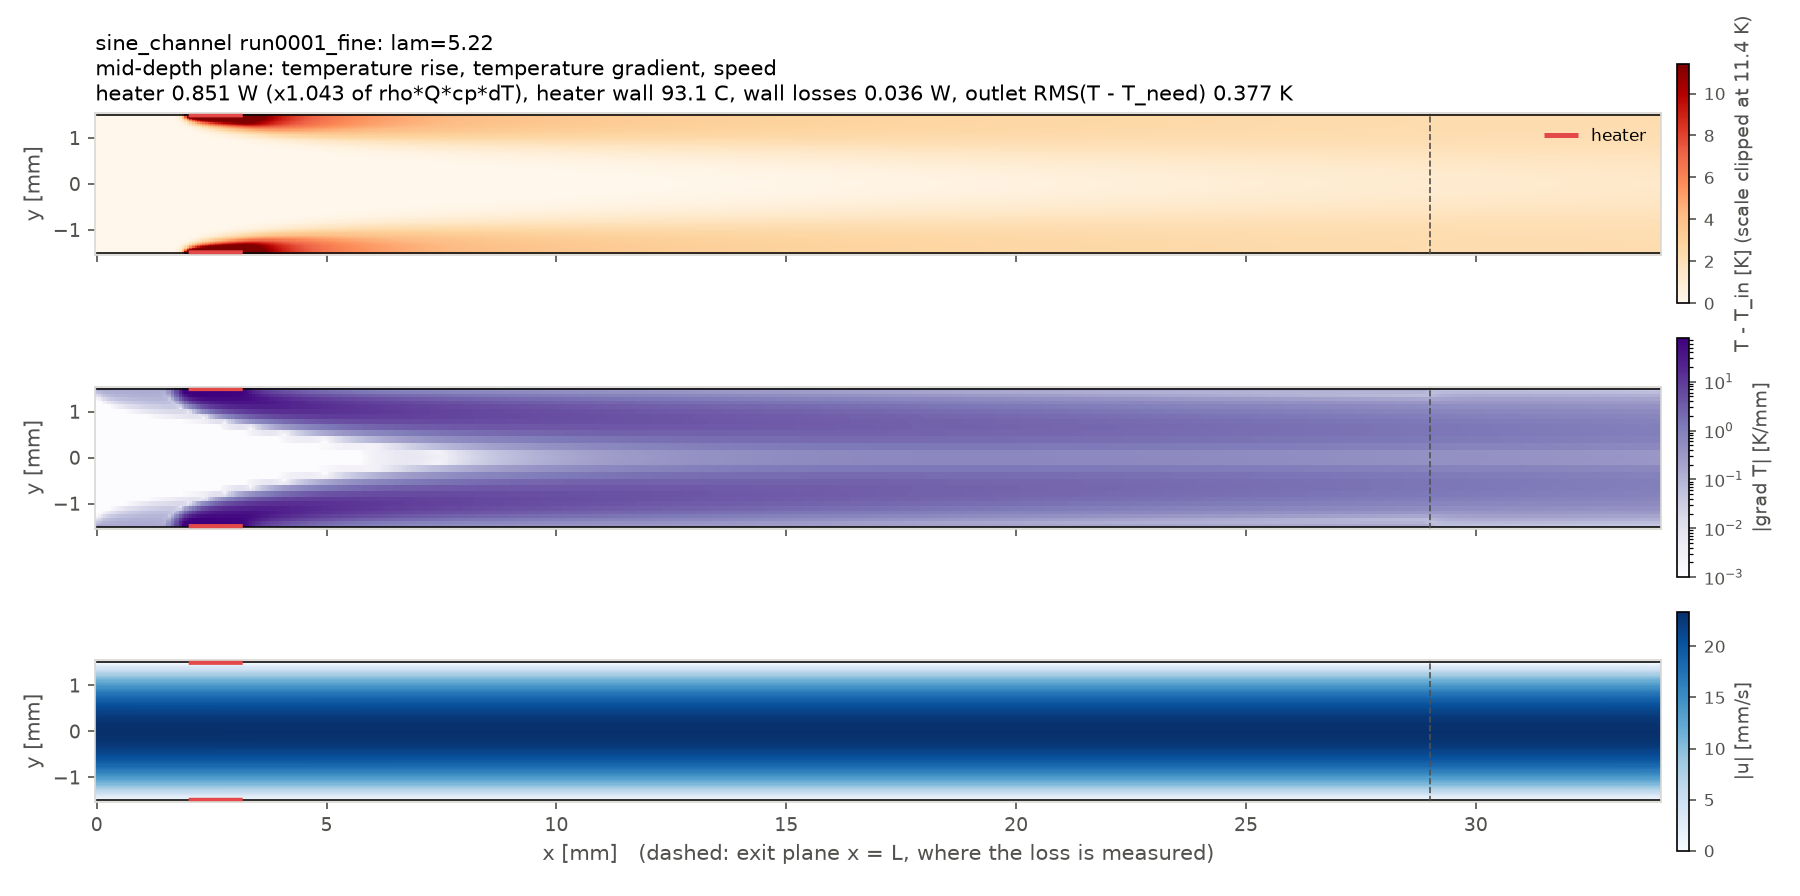
\includegraphics[width=0.95\textwidth,height=0.8\textheight,keepaspectratio]{runs/final_u3d_straight_ref_maps.png}
\caption{Temperature rise, temperature gradient and speed (mid-depth plane in 3D). Red: heated wall. The title's ``outlet RMS'' is the area-weighted $\ell_{2,\mathrm{area}}$.}
\end{figure}
\begin{figure}[H]\centering
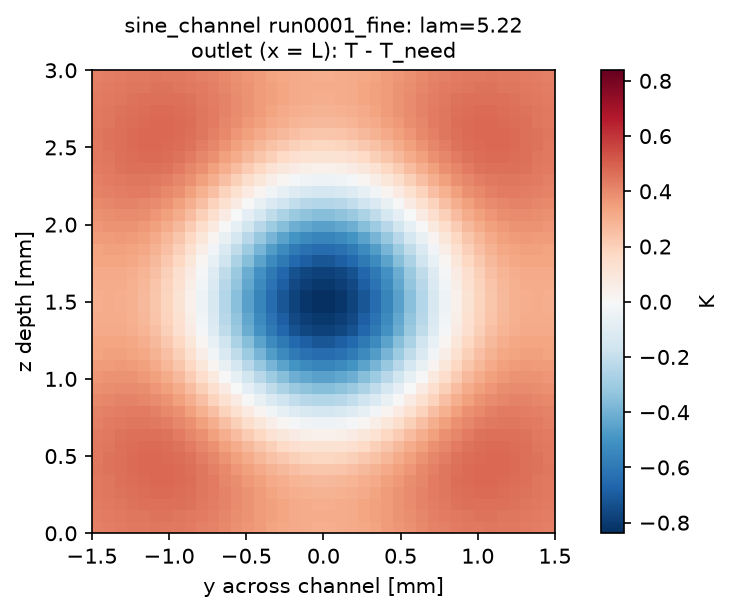
\includegraphics[width=0.75\textwidth,height=0.8\textheight,keepaspectratio]{runs/final_u3d_straight_ref_outlet.png}
\caption{Outlet temperature (and, in 3D, the outlet plane).}
\end{figure}
\begin{figure}[H]\centering
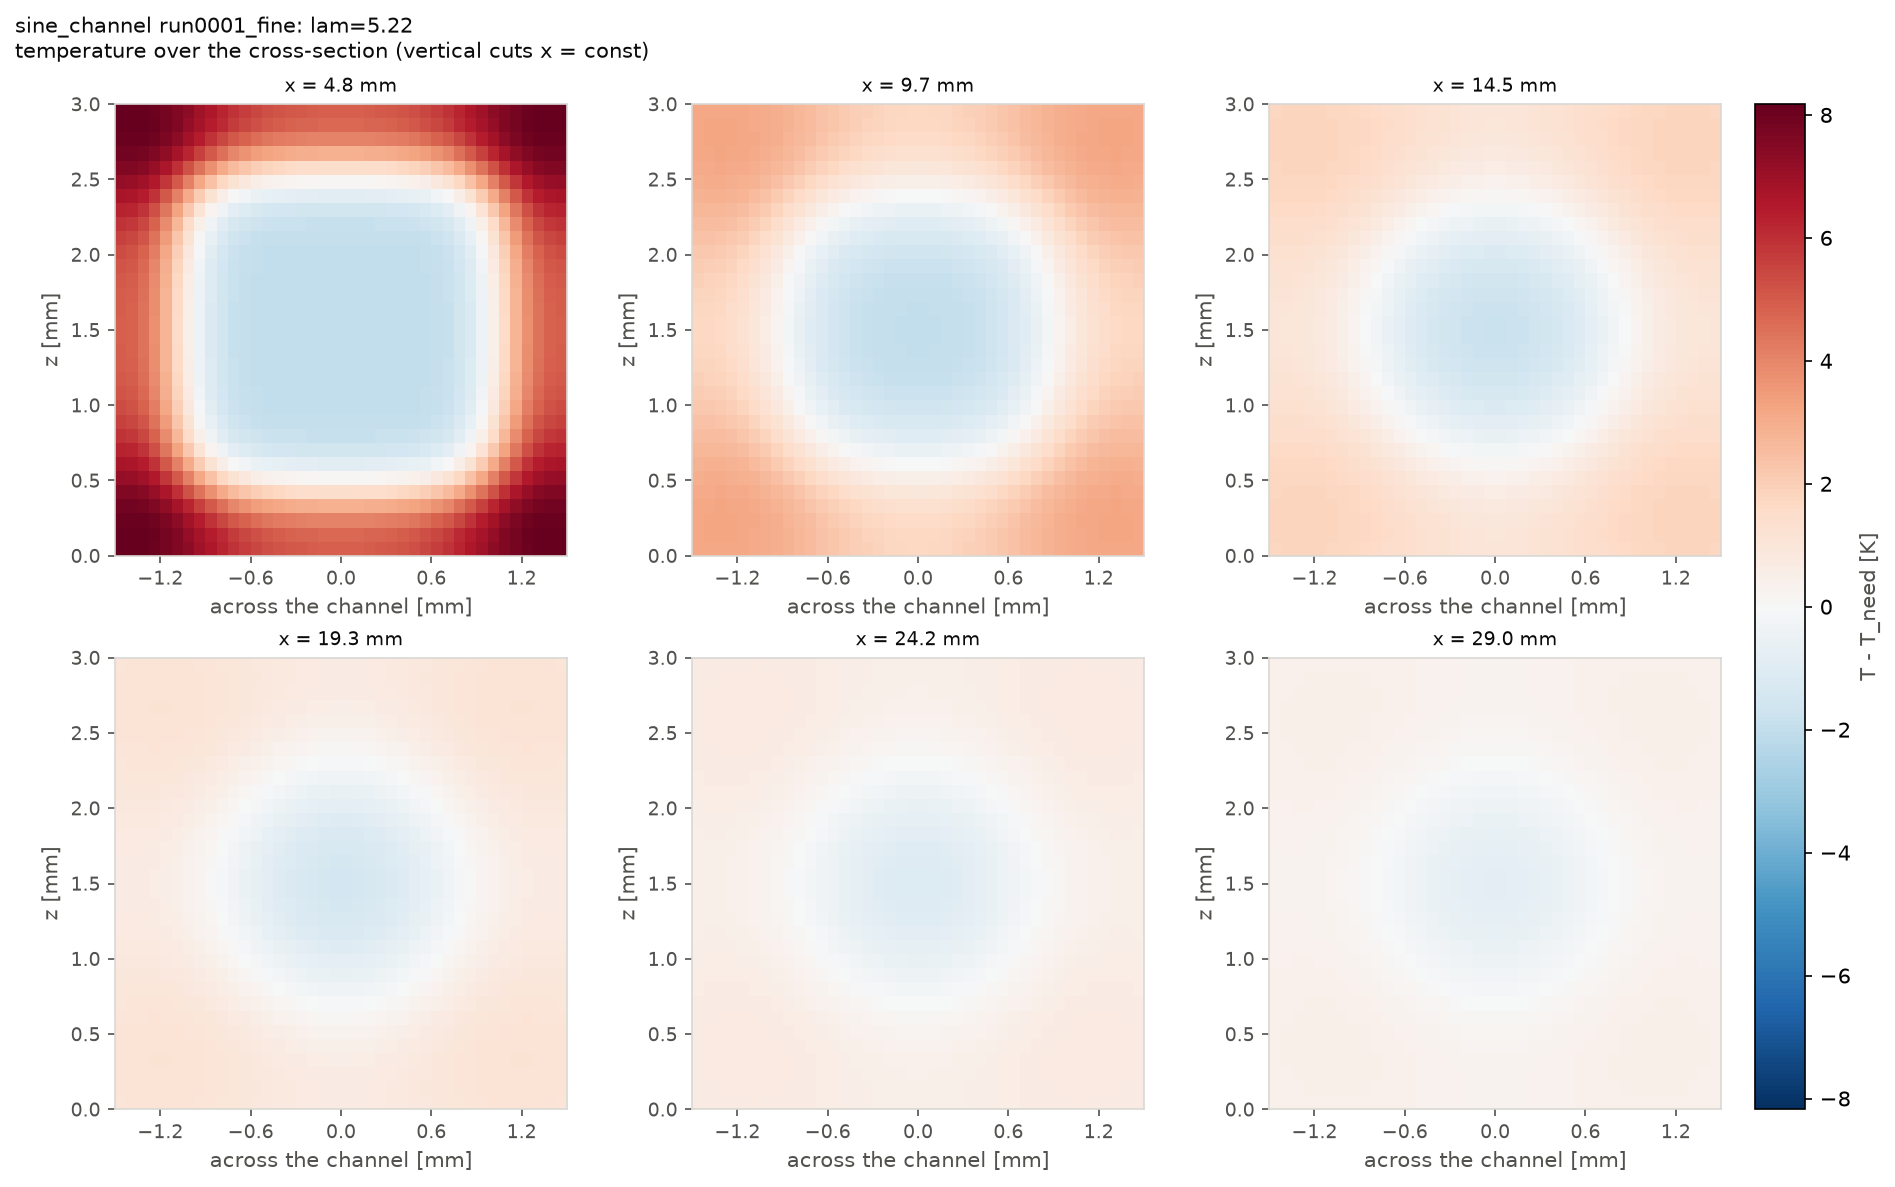
\includegraphics[width=0.62\textwidth,height=0.8\textheight,keepaspectratio]{runs/final_u3d_straight_ref_slices.png}
\caption{Temperature profiles across the channel at several $x$ stations.}
\end{figure}
\begin{figure}[H]\centering
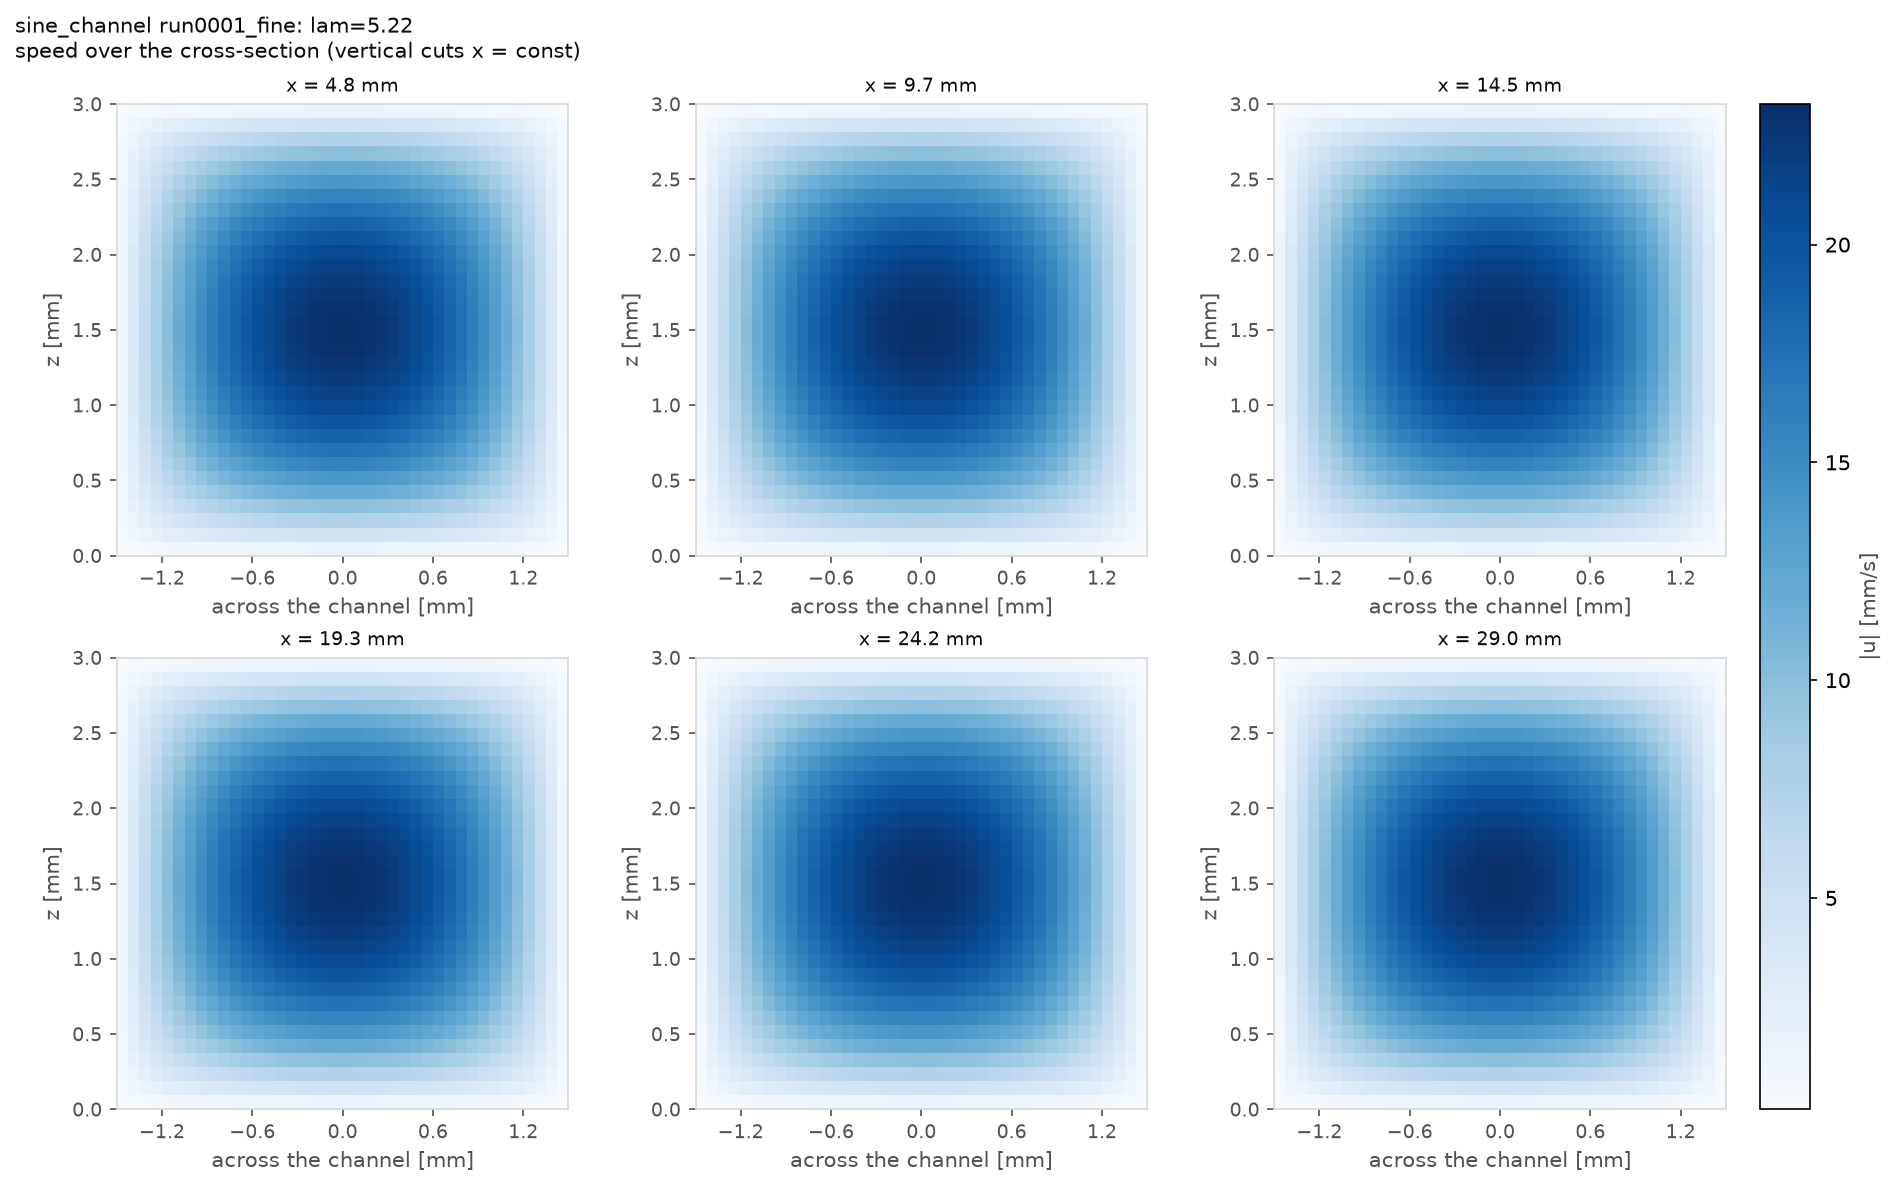
\includegraphics[width=0.85\textwidth,height=0.8\textheight,keepaspectratio]{runs/final_u3d_straight_ref_slices_u.png}
\caption{Velocity on cross-sections (3D).}
\end{figure}
\begin{figure}[H]\centering
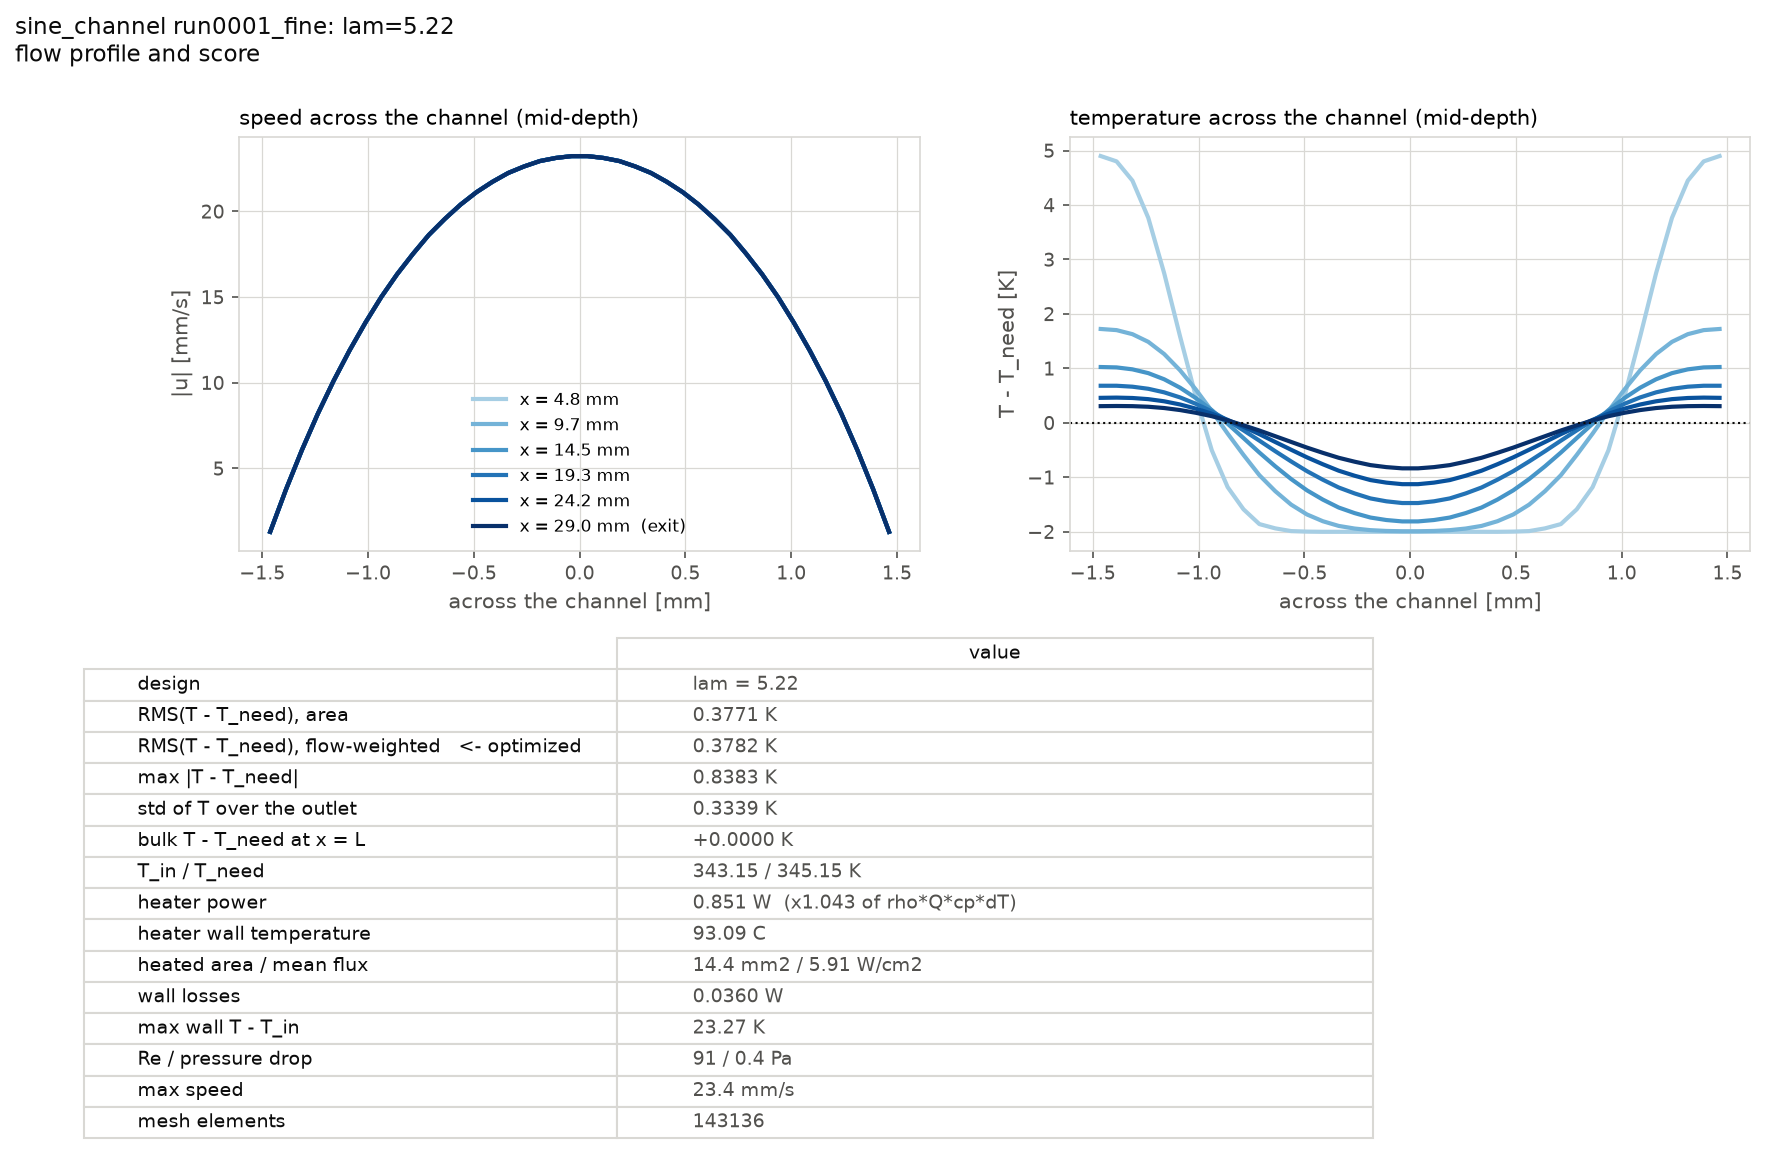
\includegraphics[width=0.8\textwidth,height=0.8\textheight,keepaspectratio]{runs/final_u3d_straight_ref_profile.png}
\caption{Speed and temperature across the channel at several $x$ stations, and the full score table of the design.}
\end{figure}
\begin{figure}[H]\centering
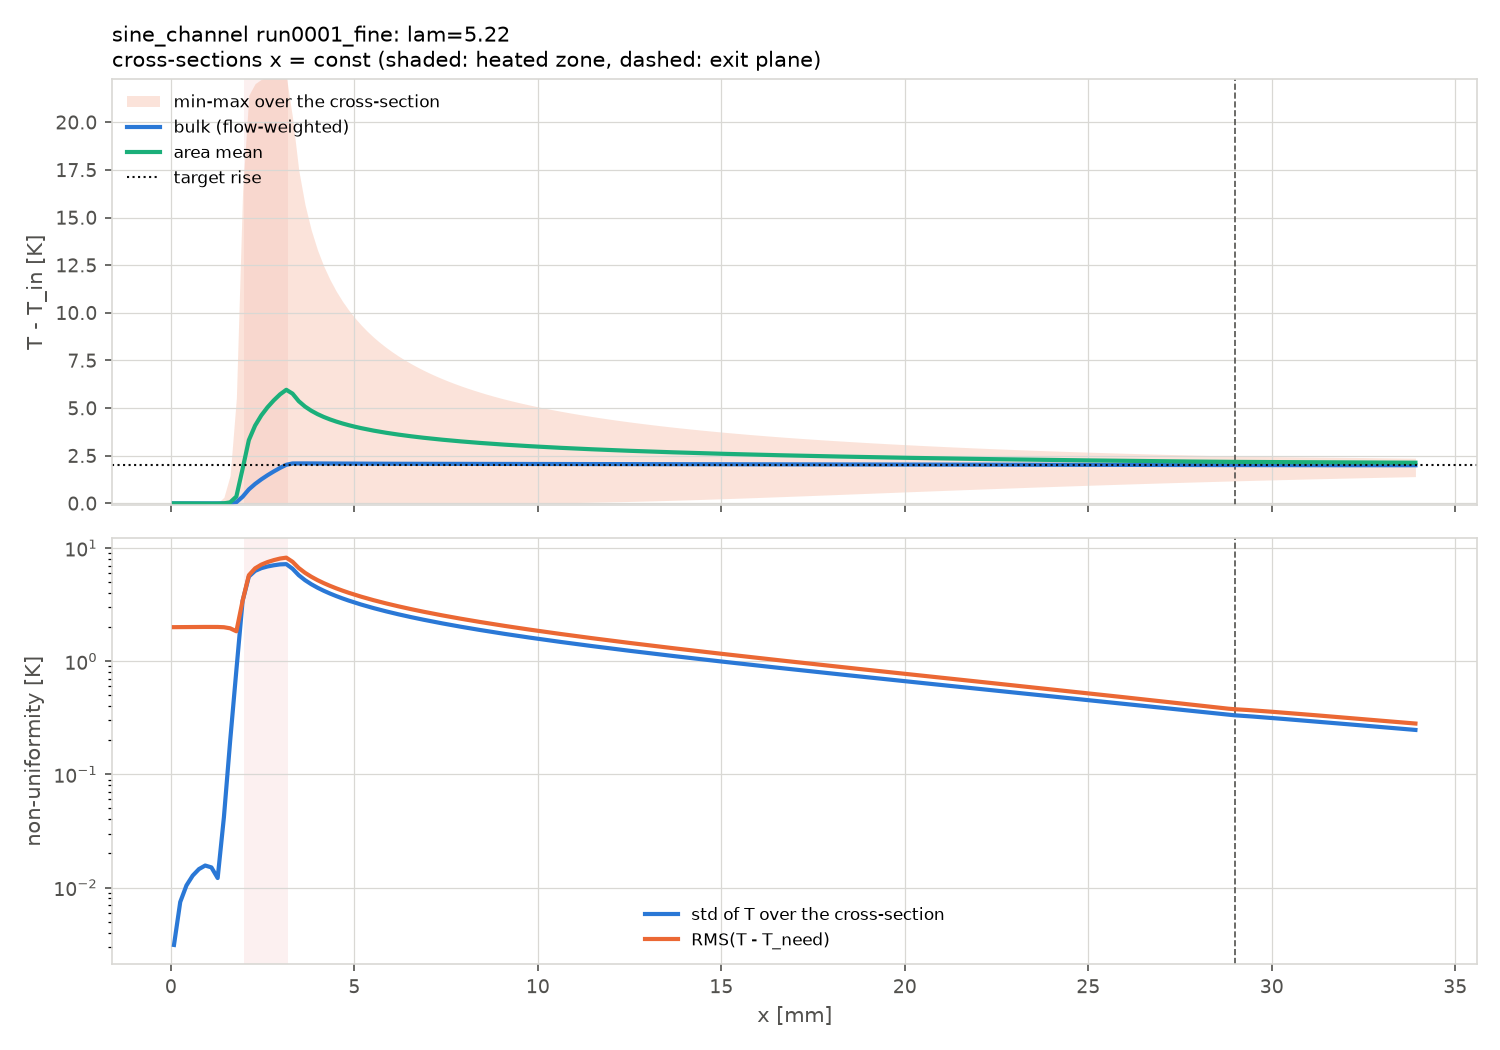
\includegraphics[width=0.8\textwidth,height=0.8\textheight,keepaspectratio]{runs/final_u3d_straight_ref_along_x.png}
\caption{Bulk, mean, min and max temperature along the channel.}
\end{figure}
\clearpage
\subsubsection*{3D serpentine, BO best \#29 ($\lambda$ 7.26, $A$ 3.5, heater 19.2\mm): 27.4\mK}
\noindent\texttt{runs/final\_u3d\_serp}\par\medskip
\begin{figure}[H]\centering
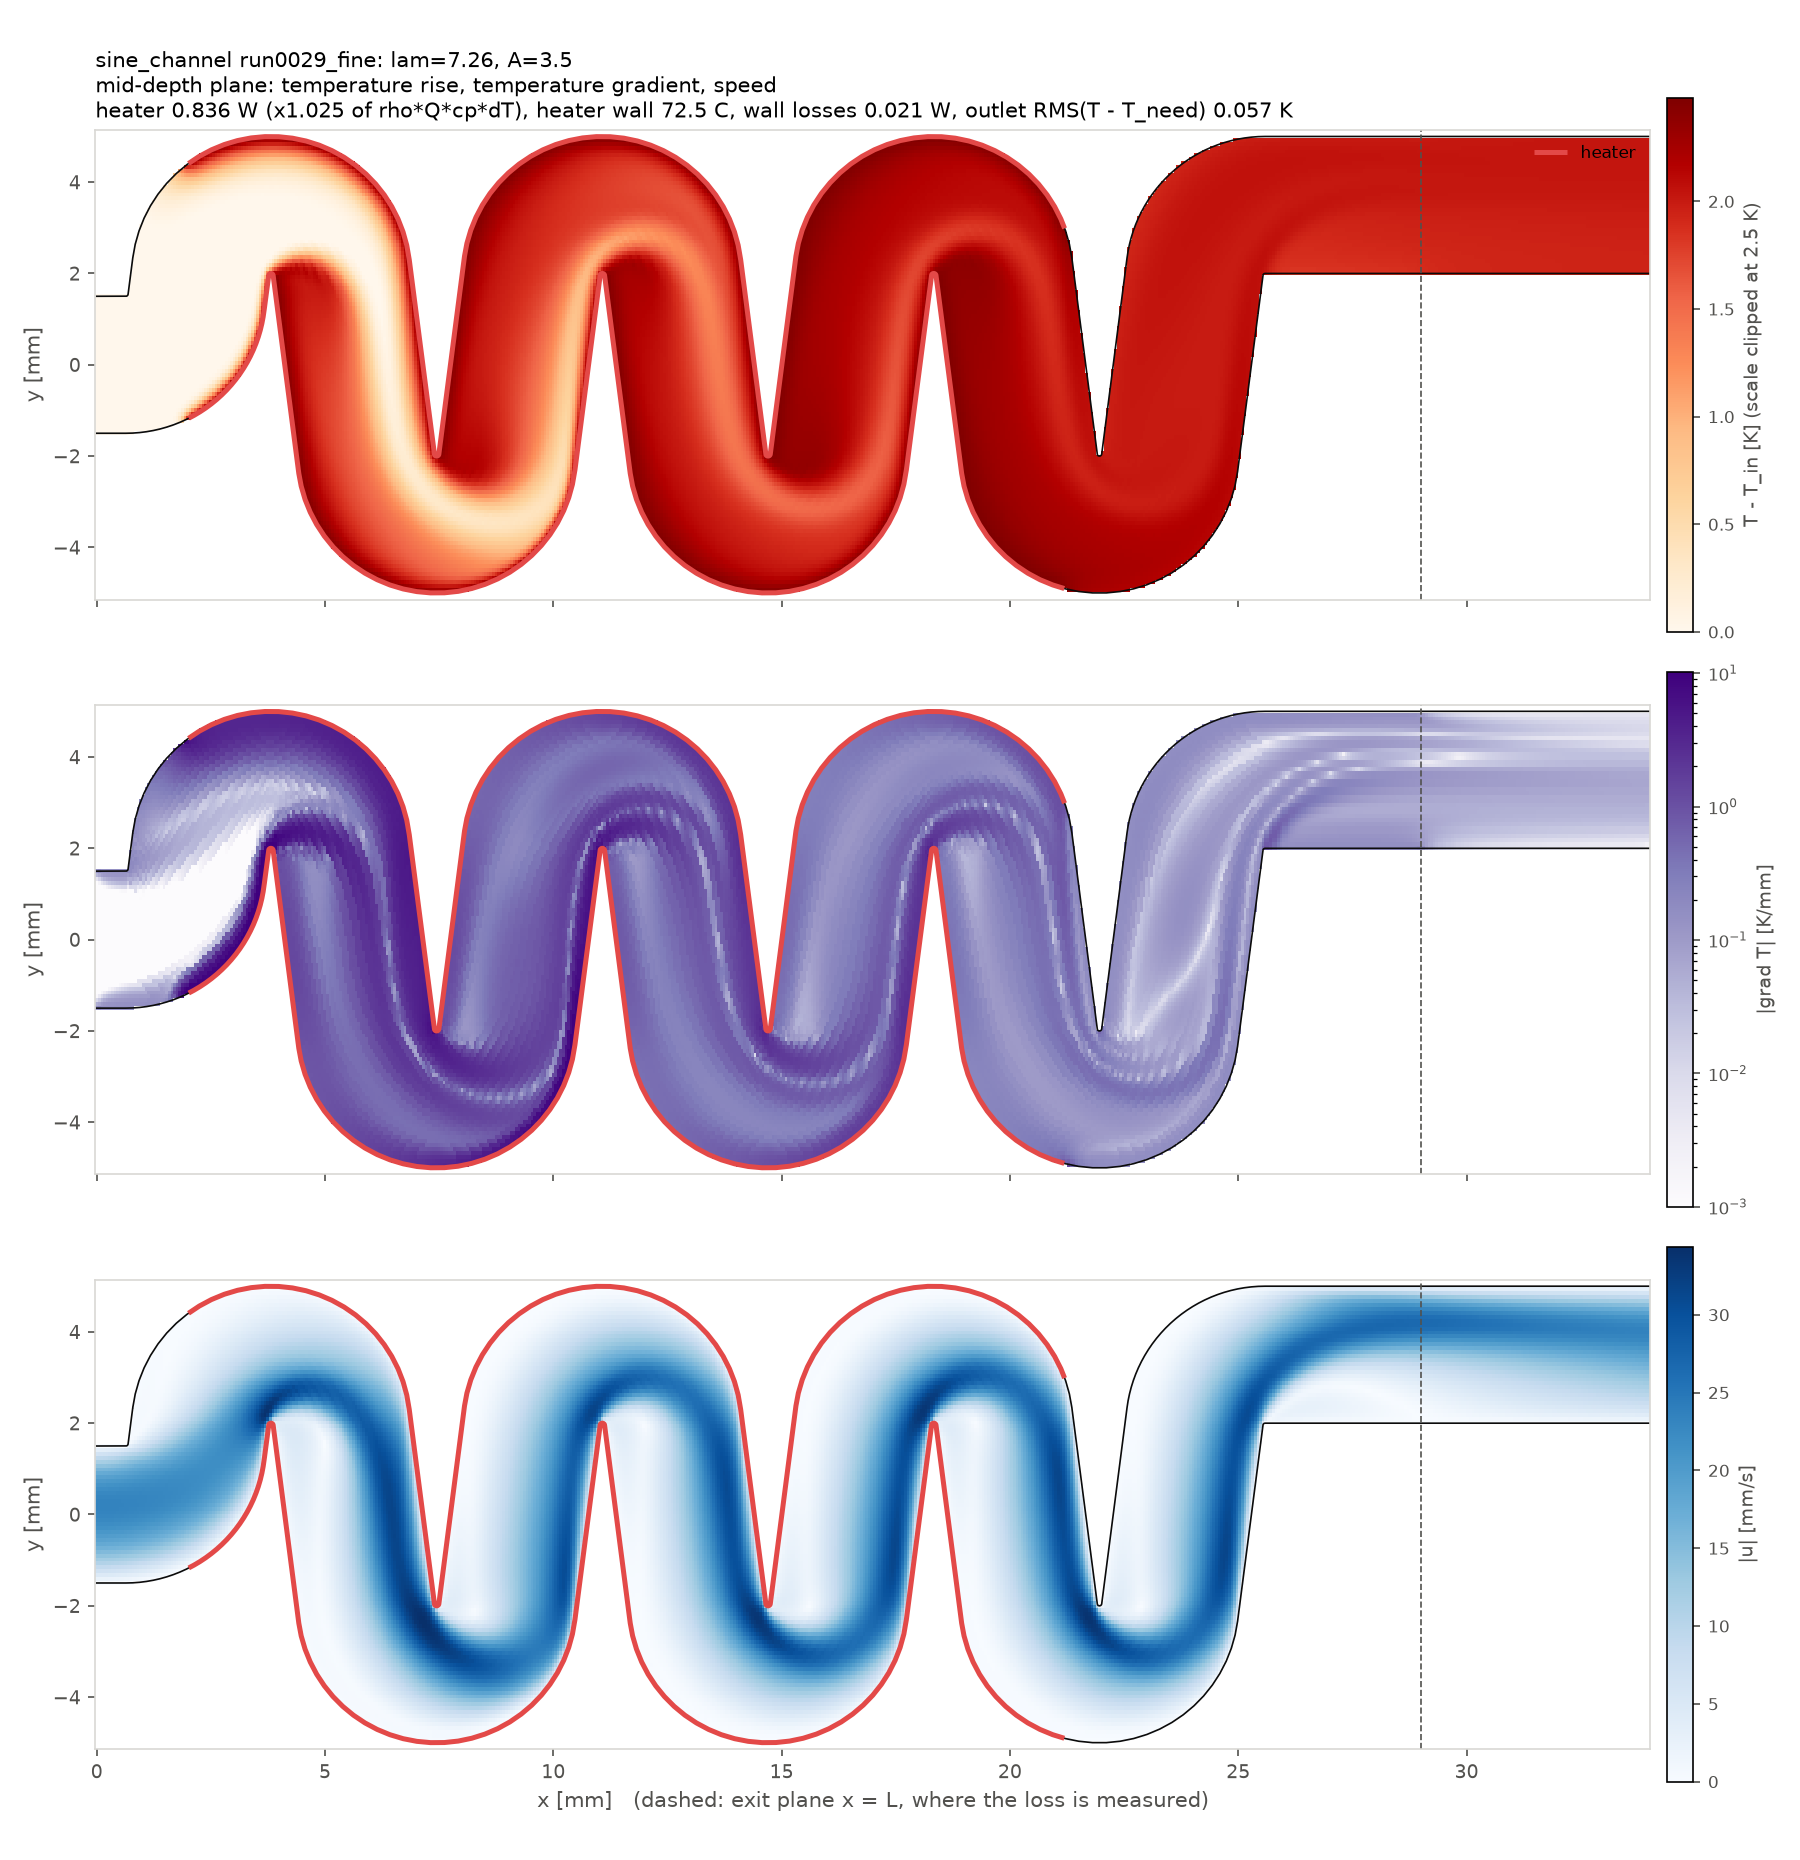
\includegraphics[width=0.95\textwidth,height=0.8\textheight,keepaspectratio]{runs/final_u3d_serp_maps.png}
\caption{Temperature rise, temperature gradient and speed (mid-depth plane in 3D). Red: heated wall. The title's ``outlet RMS'' is the area-weighted $\ell_{2,\mathrm{area}}$.}
\end{figure}
\begin{figure}[H]\centering
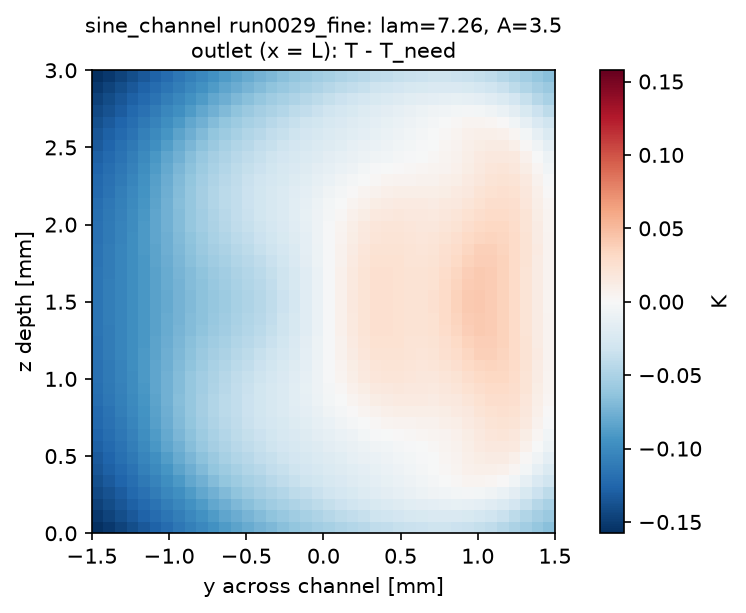
\includegraphics[width=0.75\textwidth,height=0.8\textheight,keepaspectratio]{runs/final_u3d_serp_outlet.png}
\caption{Outlet temperature (and, in 3D, the outlet plane).}
\end{figure}
\begin{figure}[H]\centering
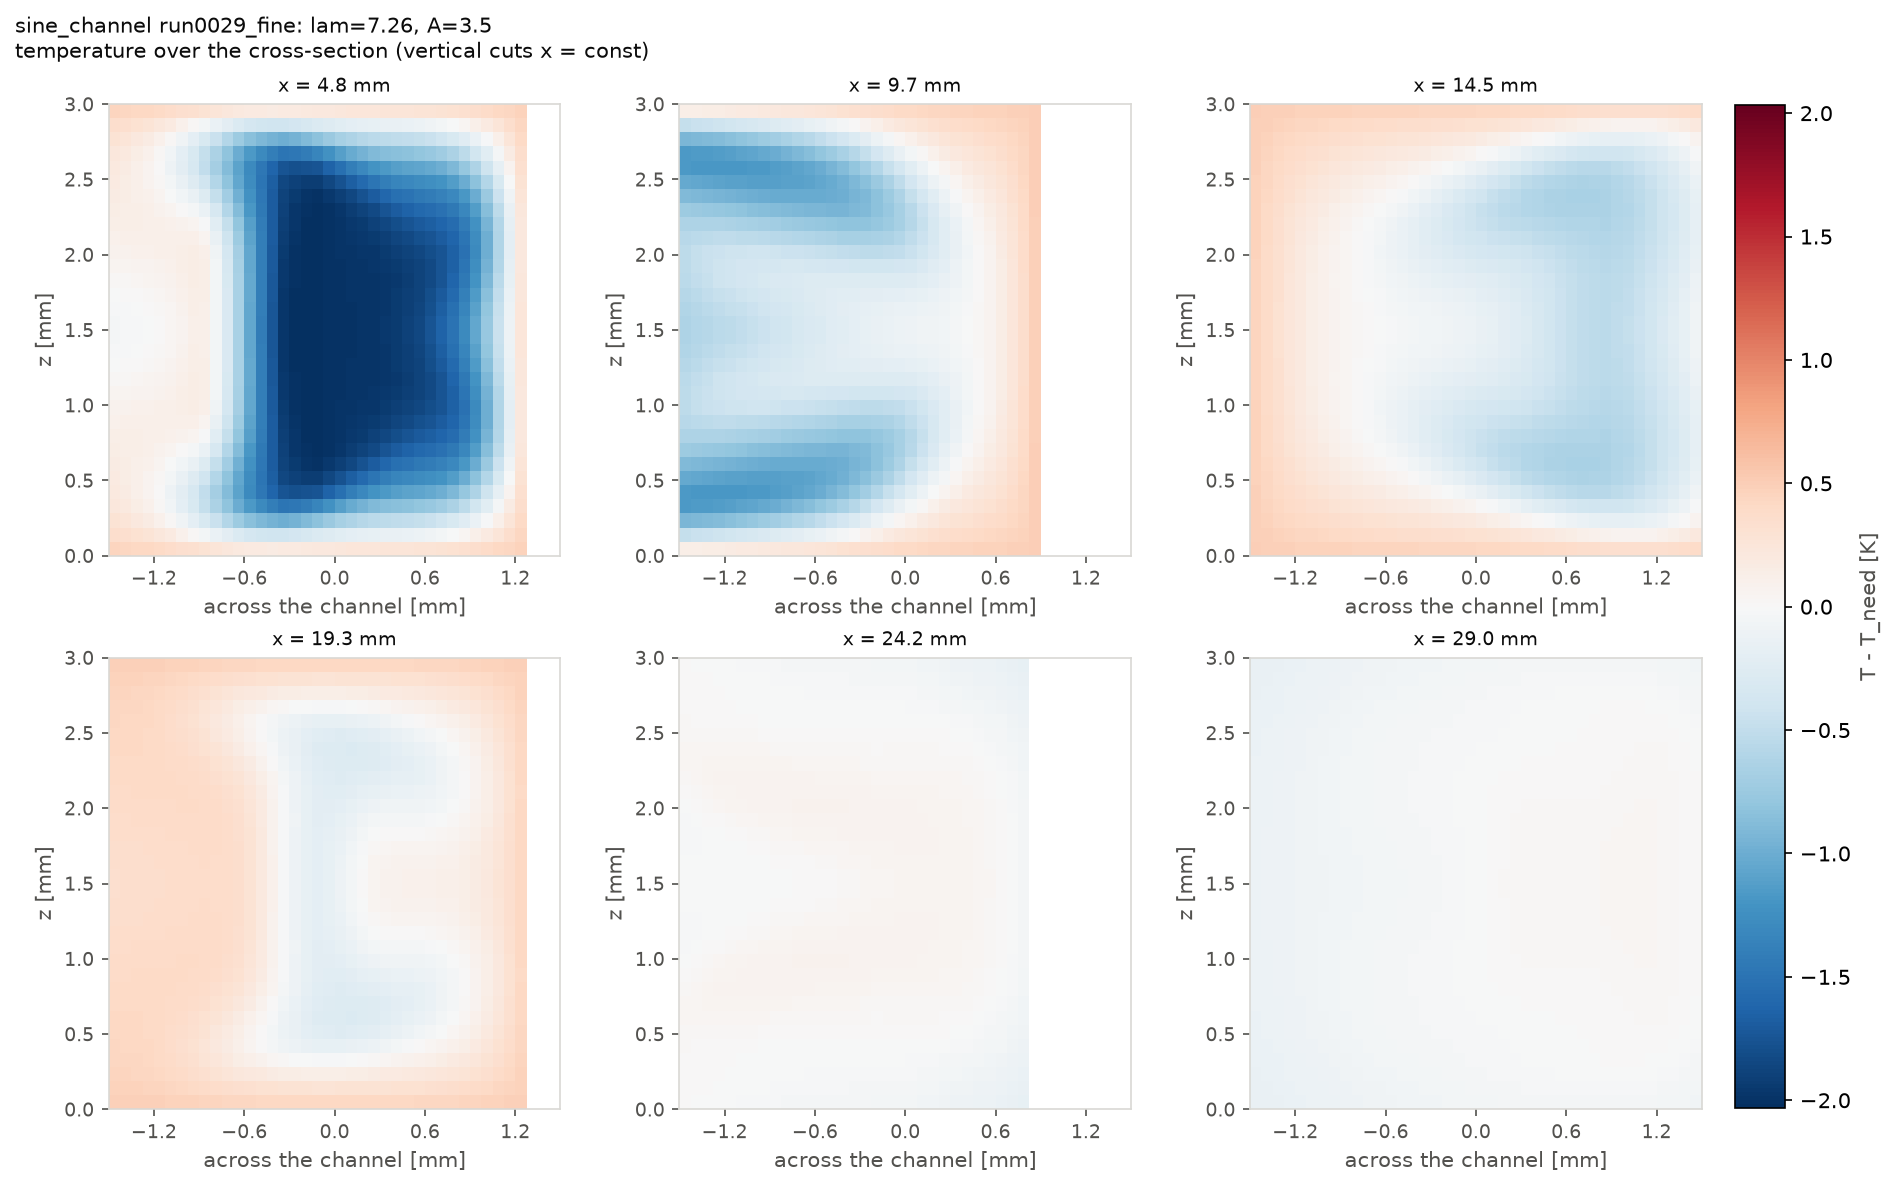
\includegraphics[width=0.62\textwidth,height=0.8\textheight,keepaspectratio]{runs/final_u3d_serp_slices.png}
\caption{Temperature profiles across the channel at several $x$ stations.}
\end{figure}
\begin{figure}[H]\centering
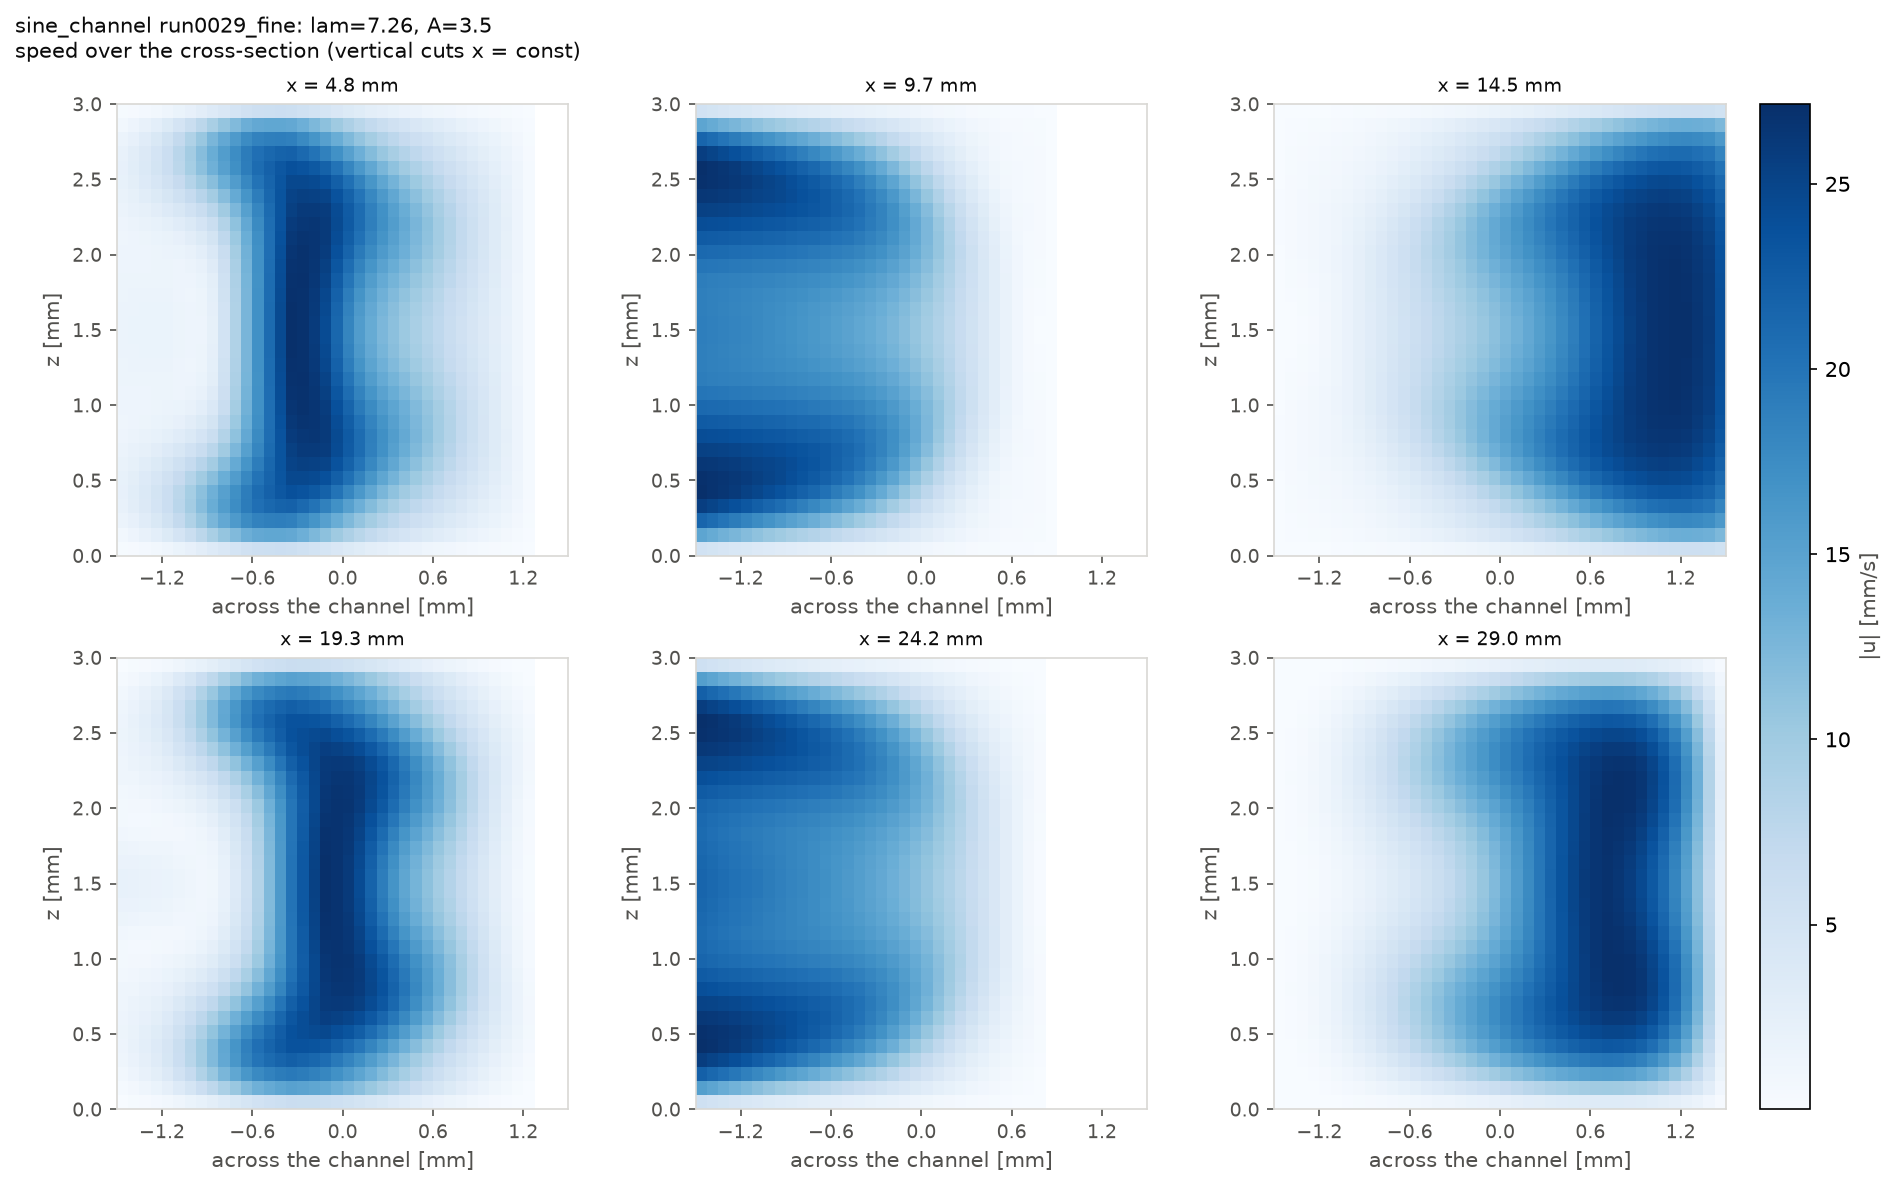
\includegraphics[width=0.85\textwidth,height=0.8\textheight,keepaspectratio]{runs/final_u3d_serp_slices_u.png}
\caption{Velocity on cross-sections (3D).}
\end{figure}
\begin{figure}[H]\centering
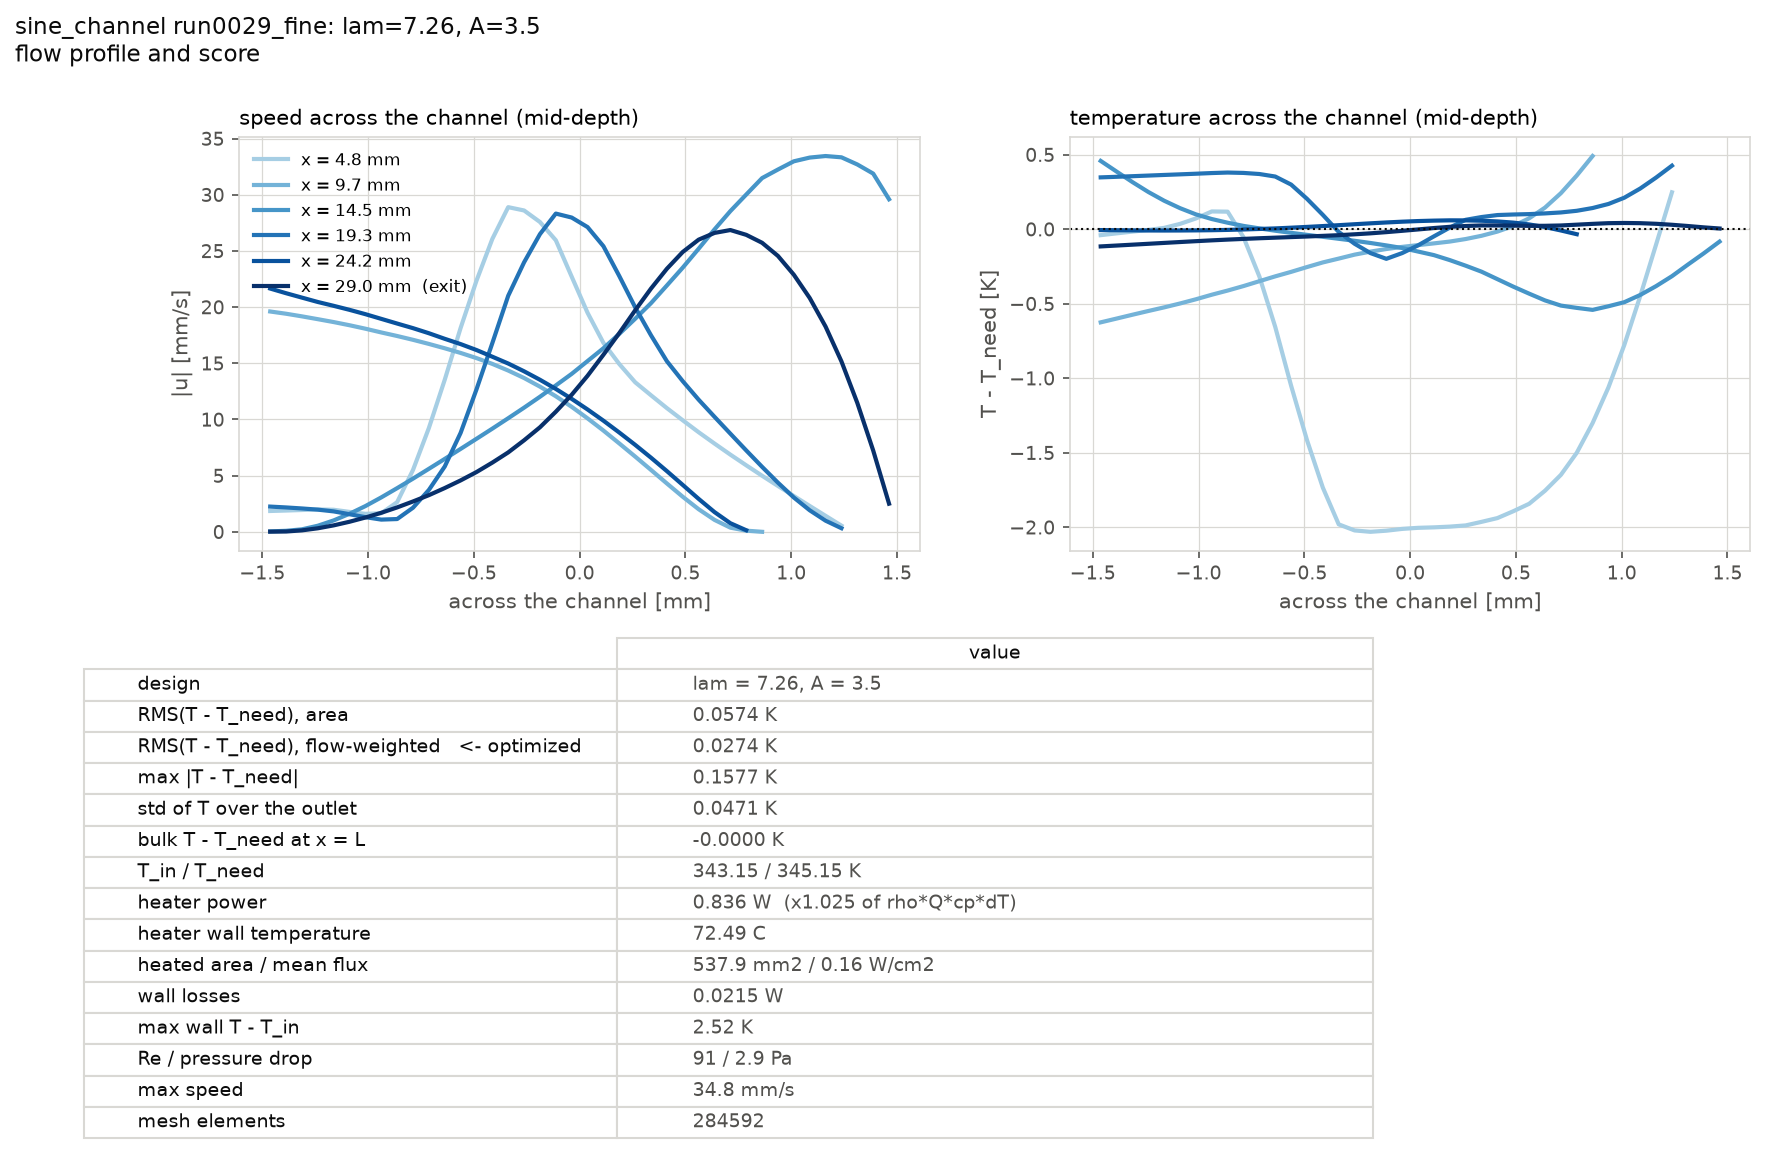
\includegraphics[width=0.8\textwidth,height=0.8\textheight,keepaspectratio]{runs/final_u3d_serp_profile.png}
\caption{Speed and temperature across the channel at several $x$ stations, and the full score table of the design.}
\end{figure}
\begin{figure}[H]\centering
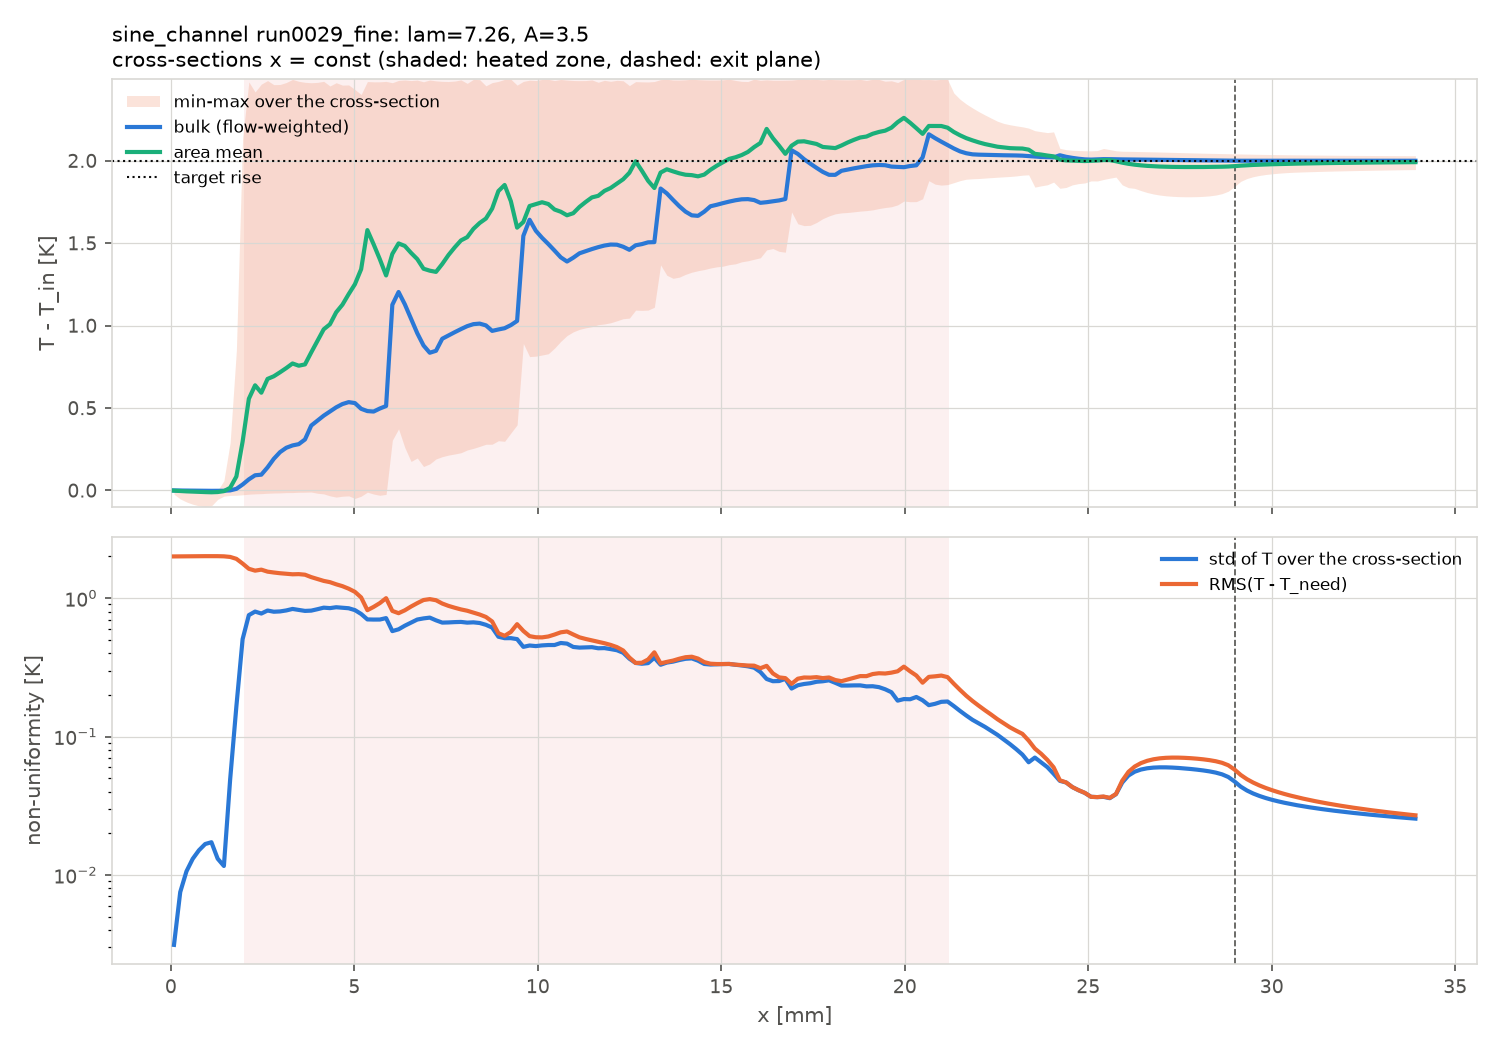
\includegraphics[width=0.8\textwidth,height=0.8\textheight,keepaspectratio]{runs/final_u3d_serp_along_x.png}
\caption{Bulk, mean, min and max temperature along the channel.}
\end{figure}
\begin{figure}[H]\centering
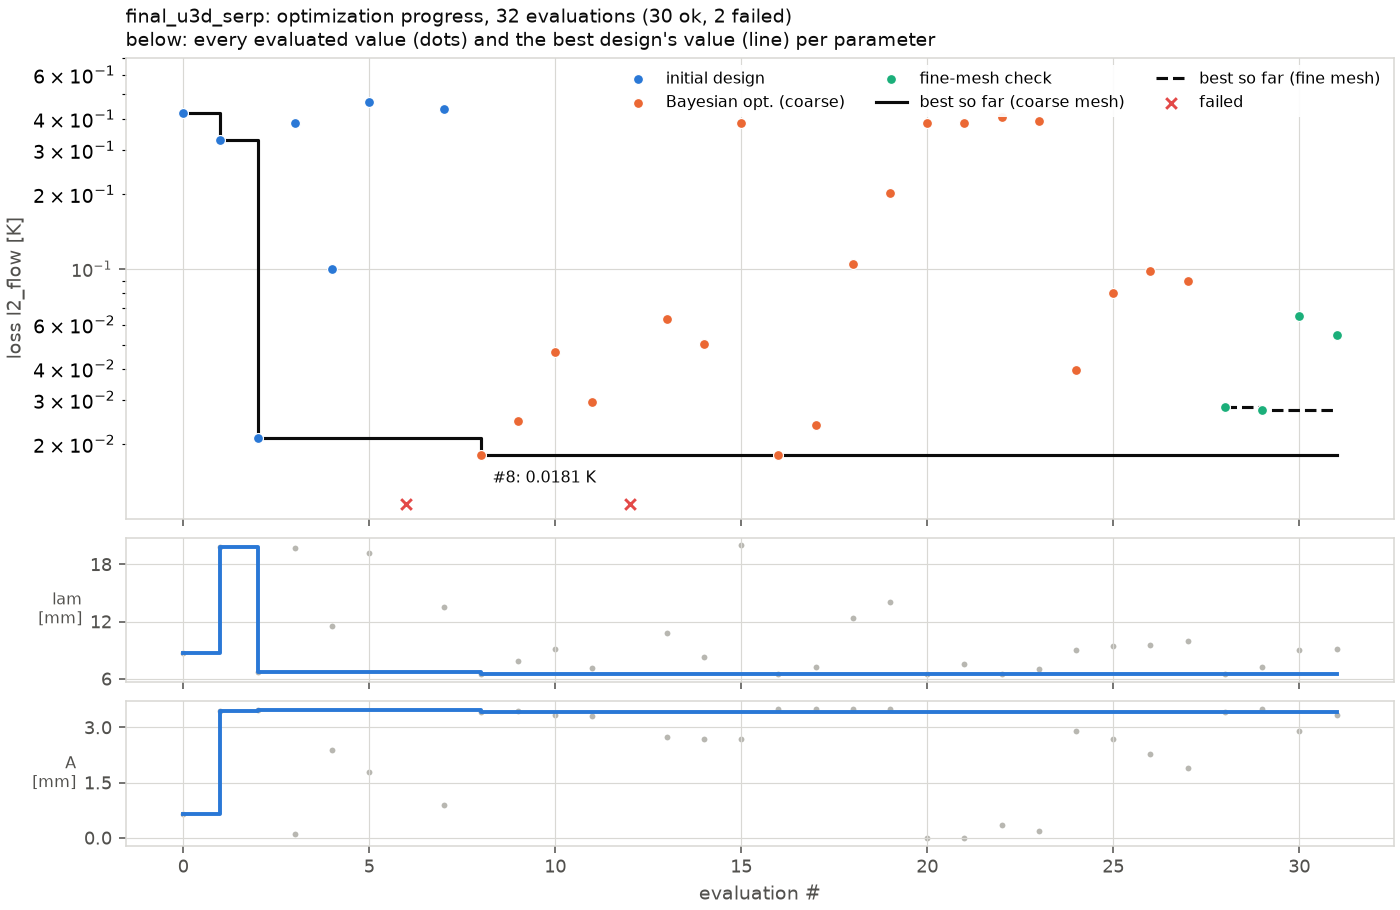
\includegraphics[width=0.85\textwidth]{runs/final_u3d_serp_progress_loss.png}
\caption{Search history: loss of every evaluation, best so far, and the parameters.}
\end{figure}
\subsection{Four branches, 2D}
\clearpage
\subsubsection*{Branched straight reference, analytic openings $\rho$ 0.532, fully heated: spread 970\mK, flow 0.87\,\%}
\noindent\texttt{runs/final\_b2d\_straight\_ref}\par\medskip
\begin{figure}[H]\centering
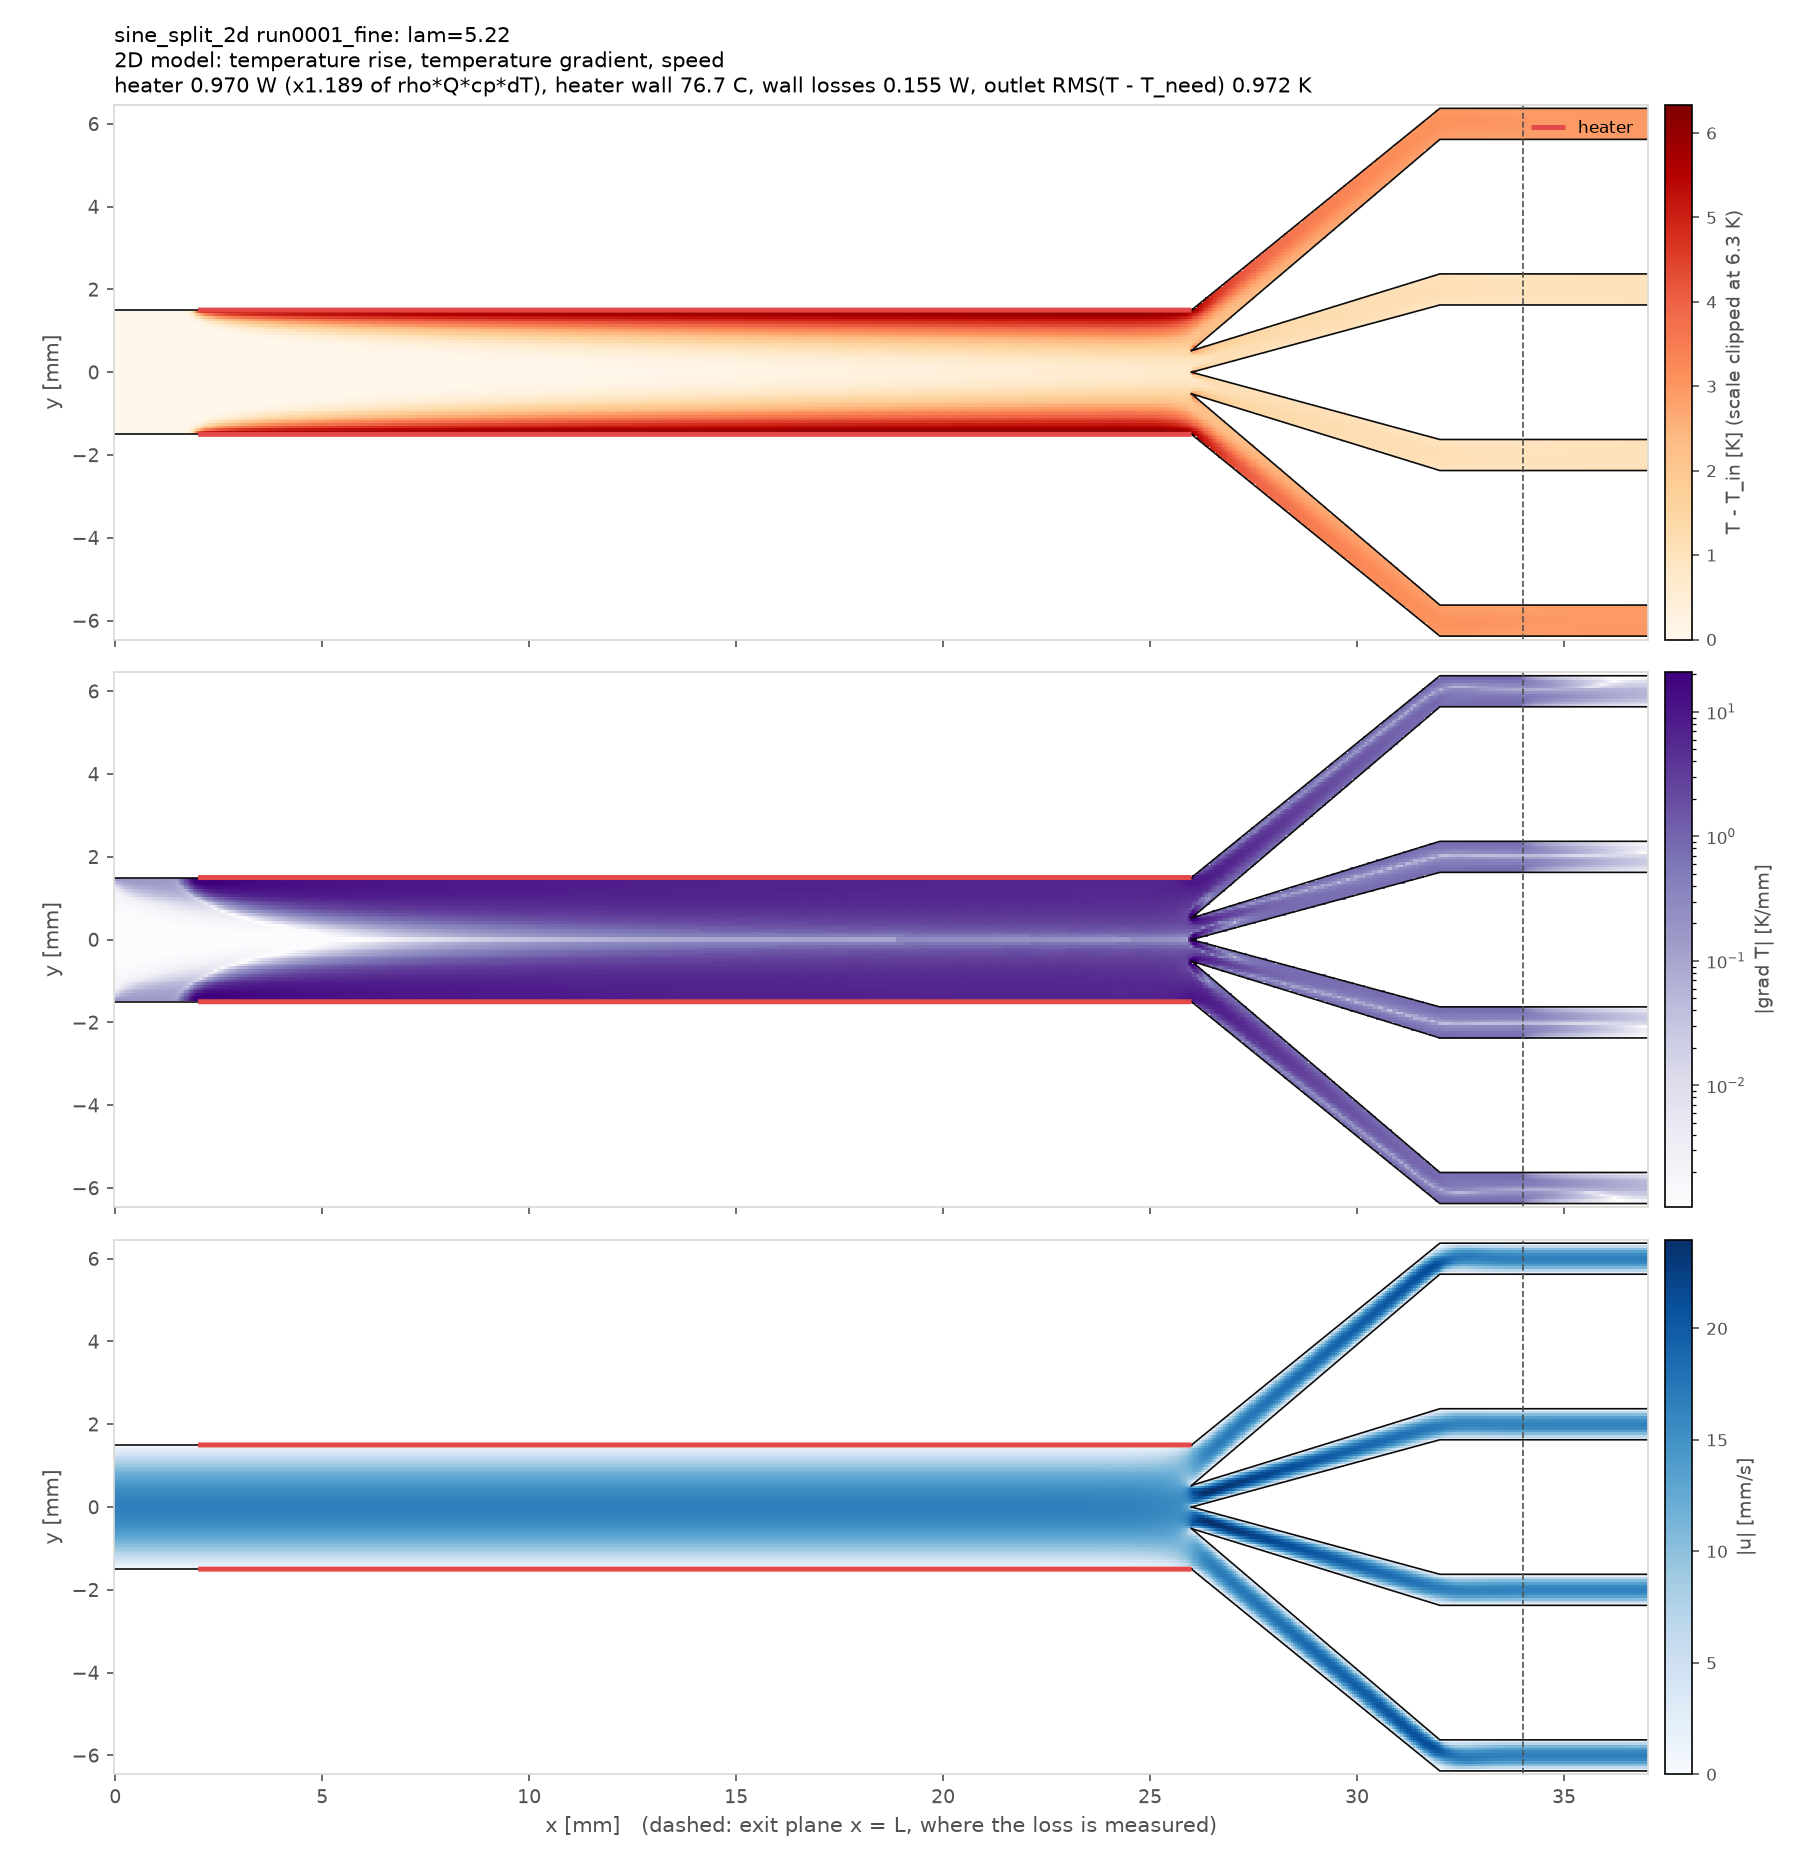
\includegraphics[width=0.95\textwidth,height=0.8\textheight,keepaspectratio]{runs/final_b2d_straight_ref_maps.png}
\caption{Temperature rise, temperature gradient and speed (mid-depth plane in 3D). Red: heated wall. The title's ``outlet RMS'' is the area-weighted $\ell_{2,\mathrm{area}}$.}
\end{figure}
\begin{figure}[H]\centering
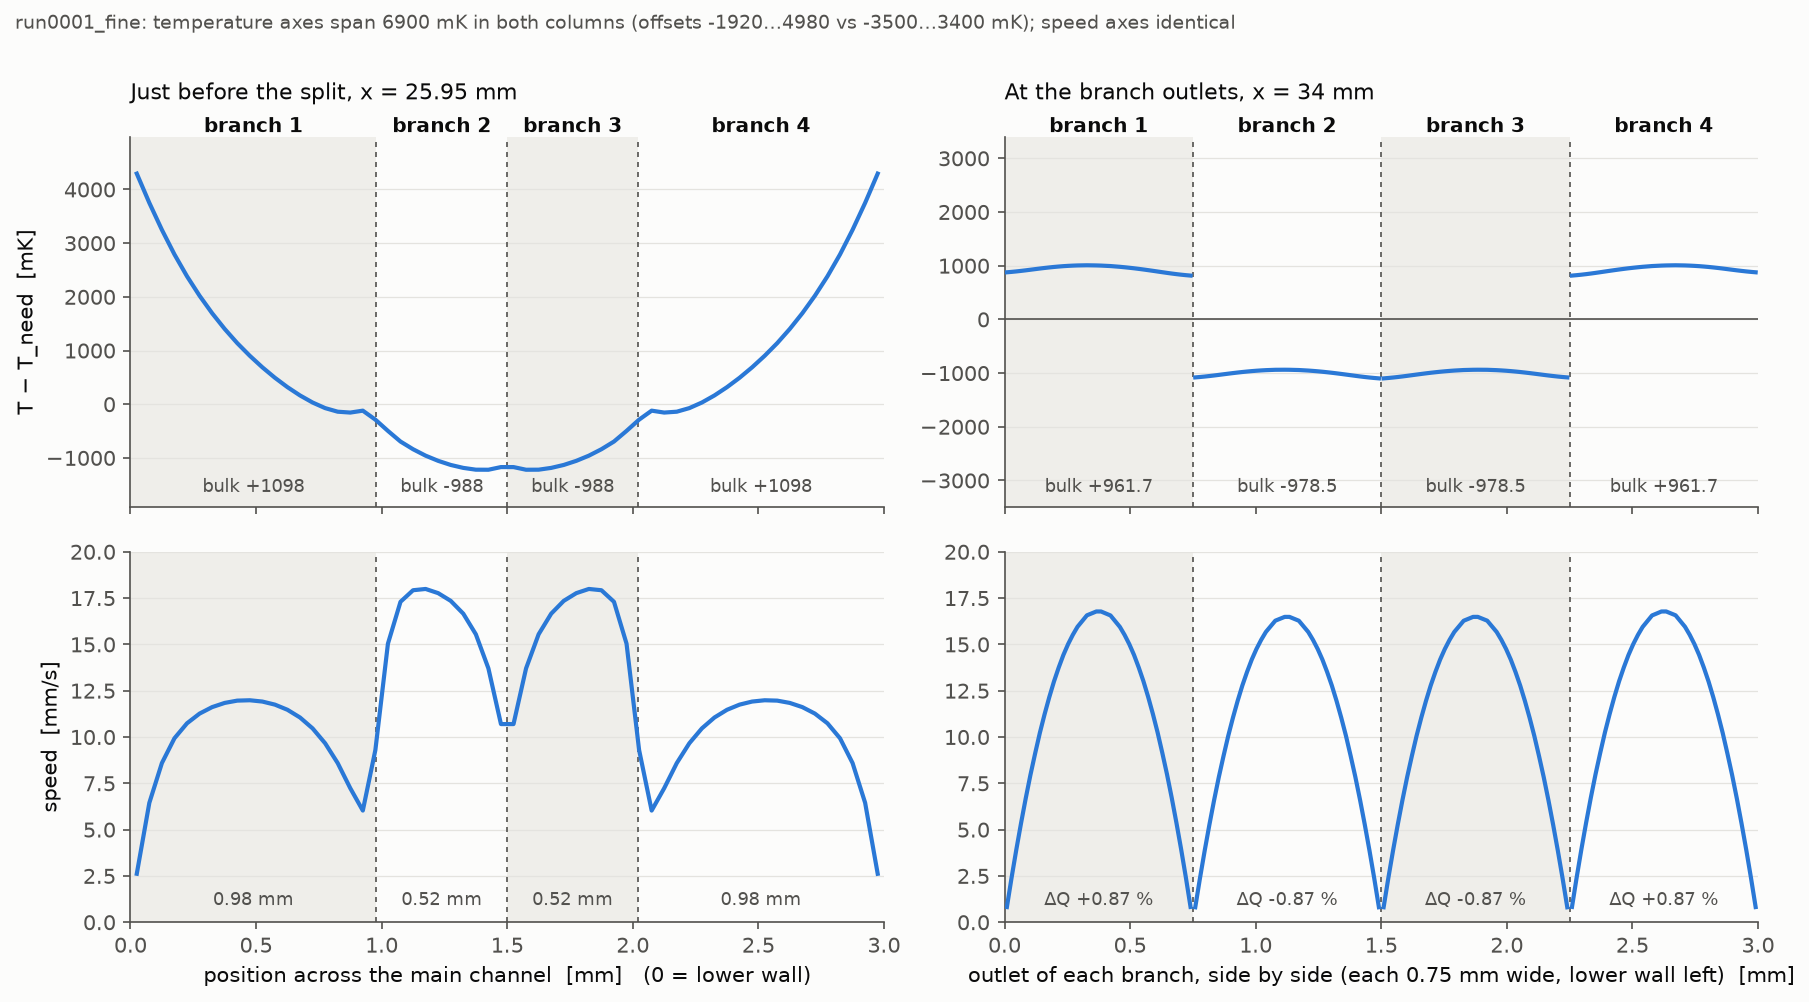
\includegraphics[width=0.95\textwidth,height=0.8\textheight,keepaspectratio]{runs/final_b2d_straight_ref_presplit.png}
\caption{Cross-section just before the split, cut into the four branch inlets, next to each branch outlet.}
\end{figure}
\begin{figure}[H]\centering
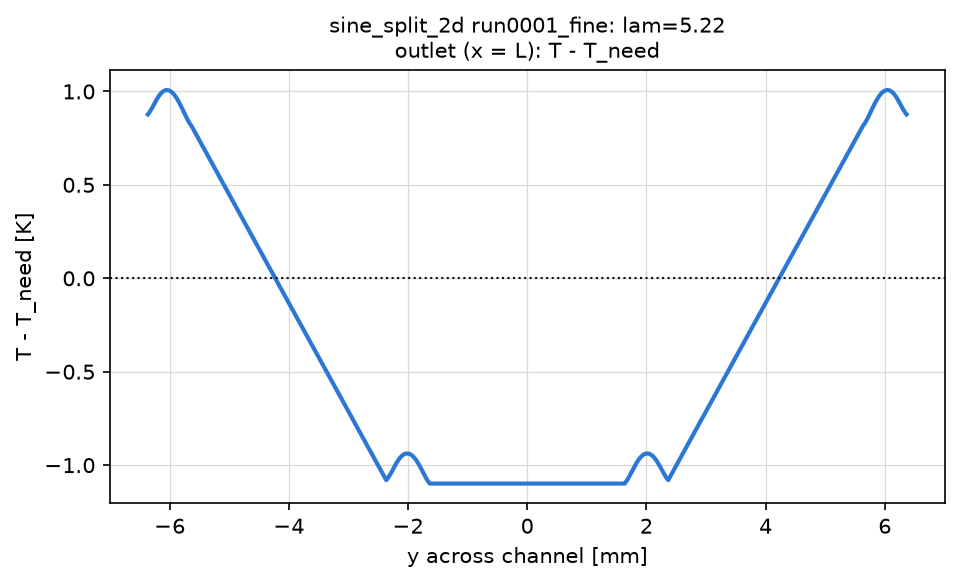
\includegraphics[width=0.75\textwidth,height=0.8\textheight,keepaspectratio]{runs/final_b2d_straight_ref_outlet.png}
\caption{Outlet temperature (and, in 3D, the outlet plane).}
\end{figure}
\begin{figure}[H]\centering
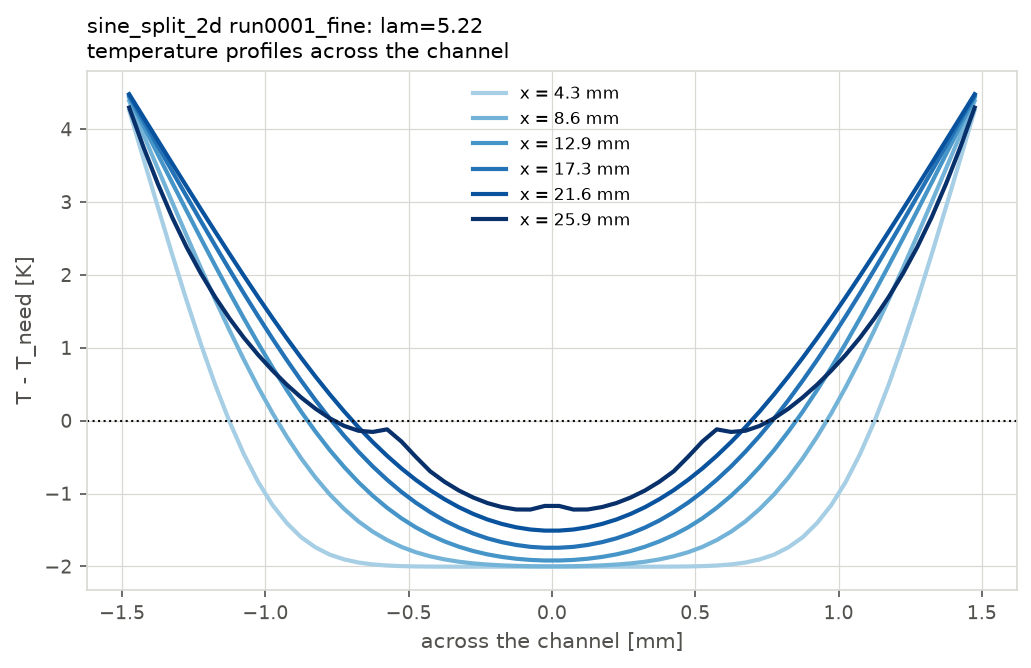
\includegraphics[width=0.62\textwidth,height=0.8\textheight,keepaspectratio]{runs/final_b2d_straight_ref_slices.png}
\caption{Temperature profiles across the channel at several $x$ stations.}
\end{figure}
\begin{figure}[H]\centering
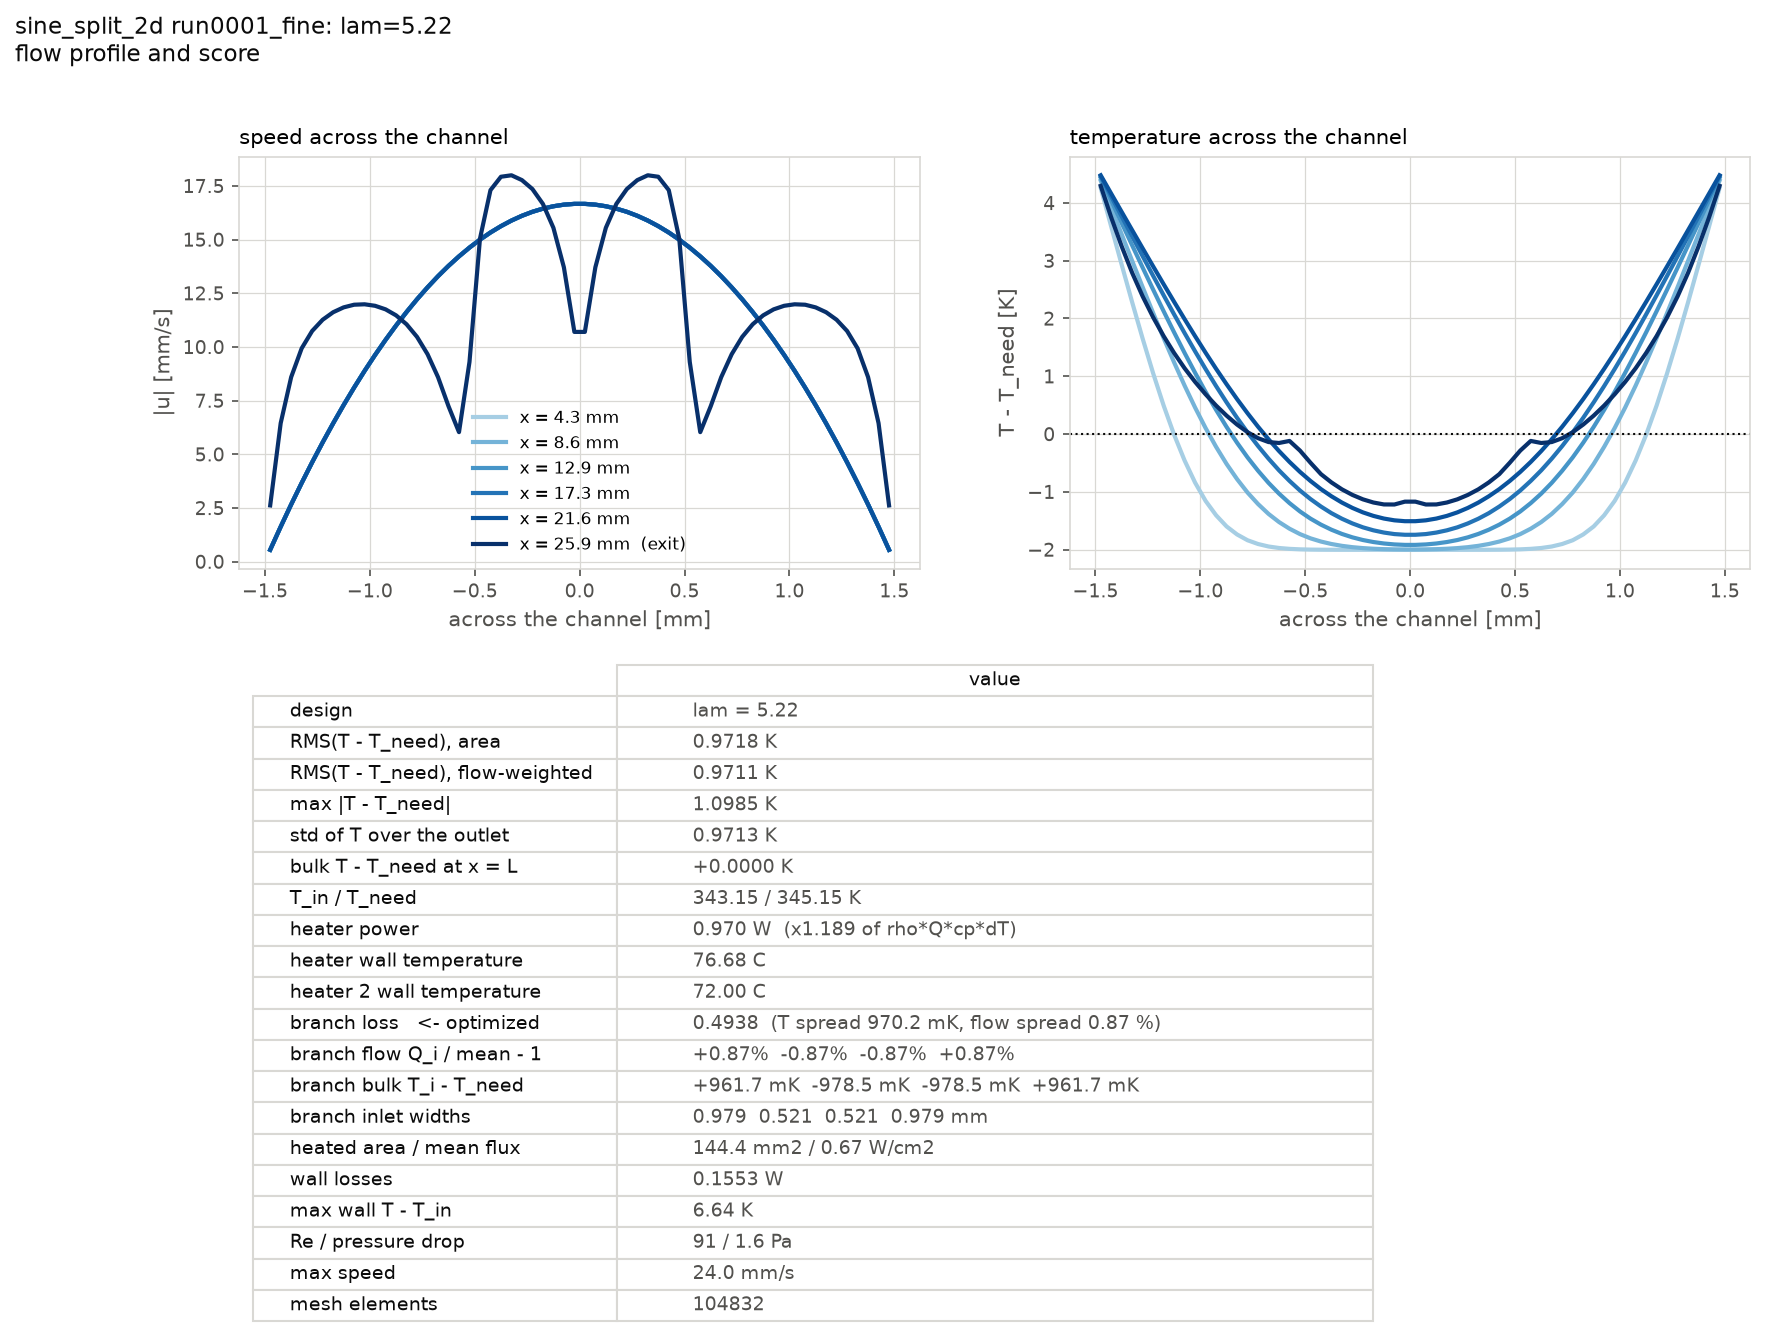
\includegraphics[width=0.8\textwidth,height=0.8\textheight,keepaspectratio]{runs/final_b2d_straight_ref_profile.png}
\caption{Speed and temperature across the channel at several $x$ stations, and the full score table of the design.}
\end{figure}
\begin{figure}[H]\centering
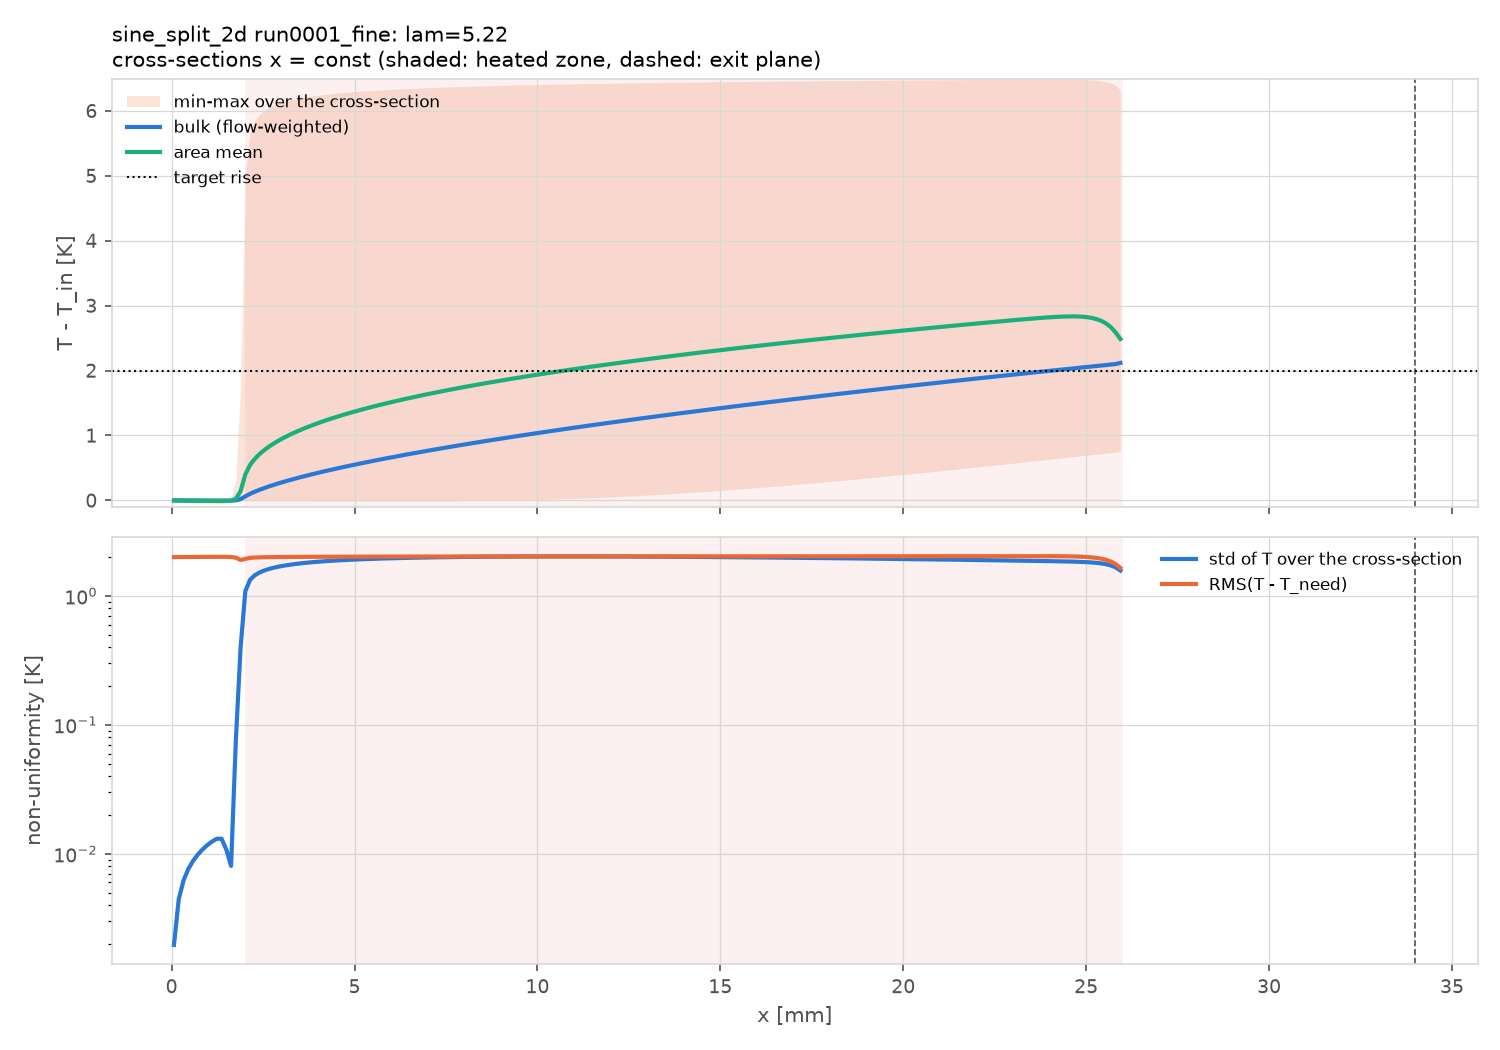
\includegraphics[width=0.8\textwidth,height=0.8\textheight,keepaspectratio]{runs/final_b2d_straight_ref_along_x.png}
\caption{Bulk, mean, min and max temperature along the channel.}
\end{figure}
\clearpage
\subsubsection*{Branched straight, BO best \#16 ($\rho$ 0.540, heater 2.4\mm, clamped at 99\,$^\circ$C): 515\mK, 0.16\,\%}
\noindent\texttt{runs/final\_b2d\_straight}\par\medskip
\begin{figure}[H]\centering
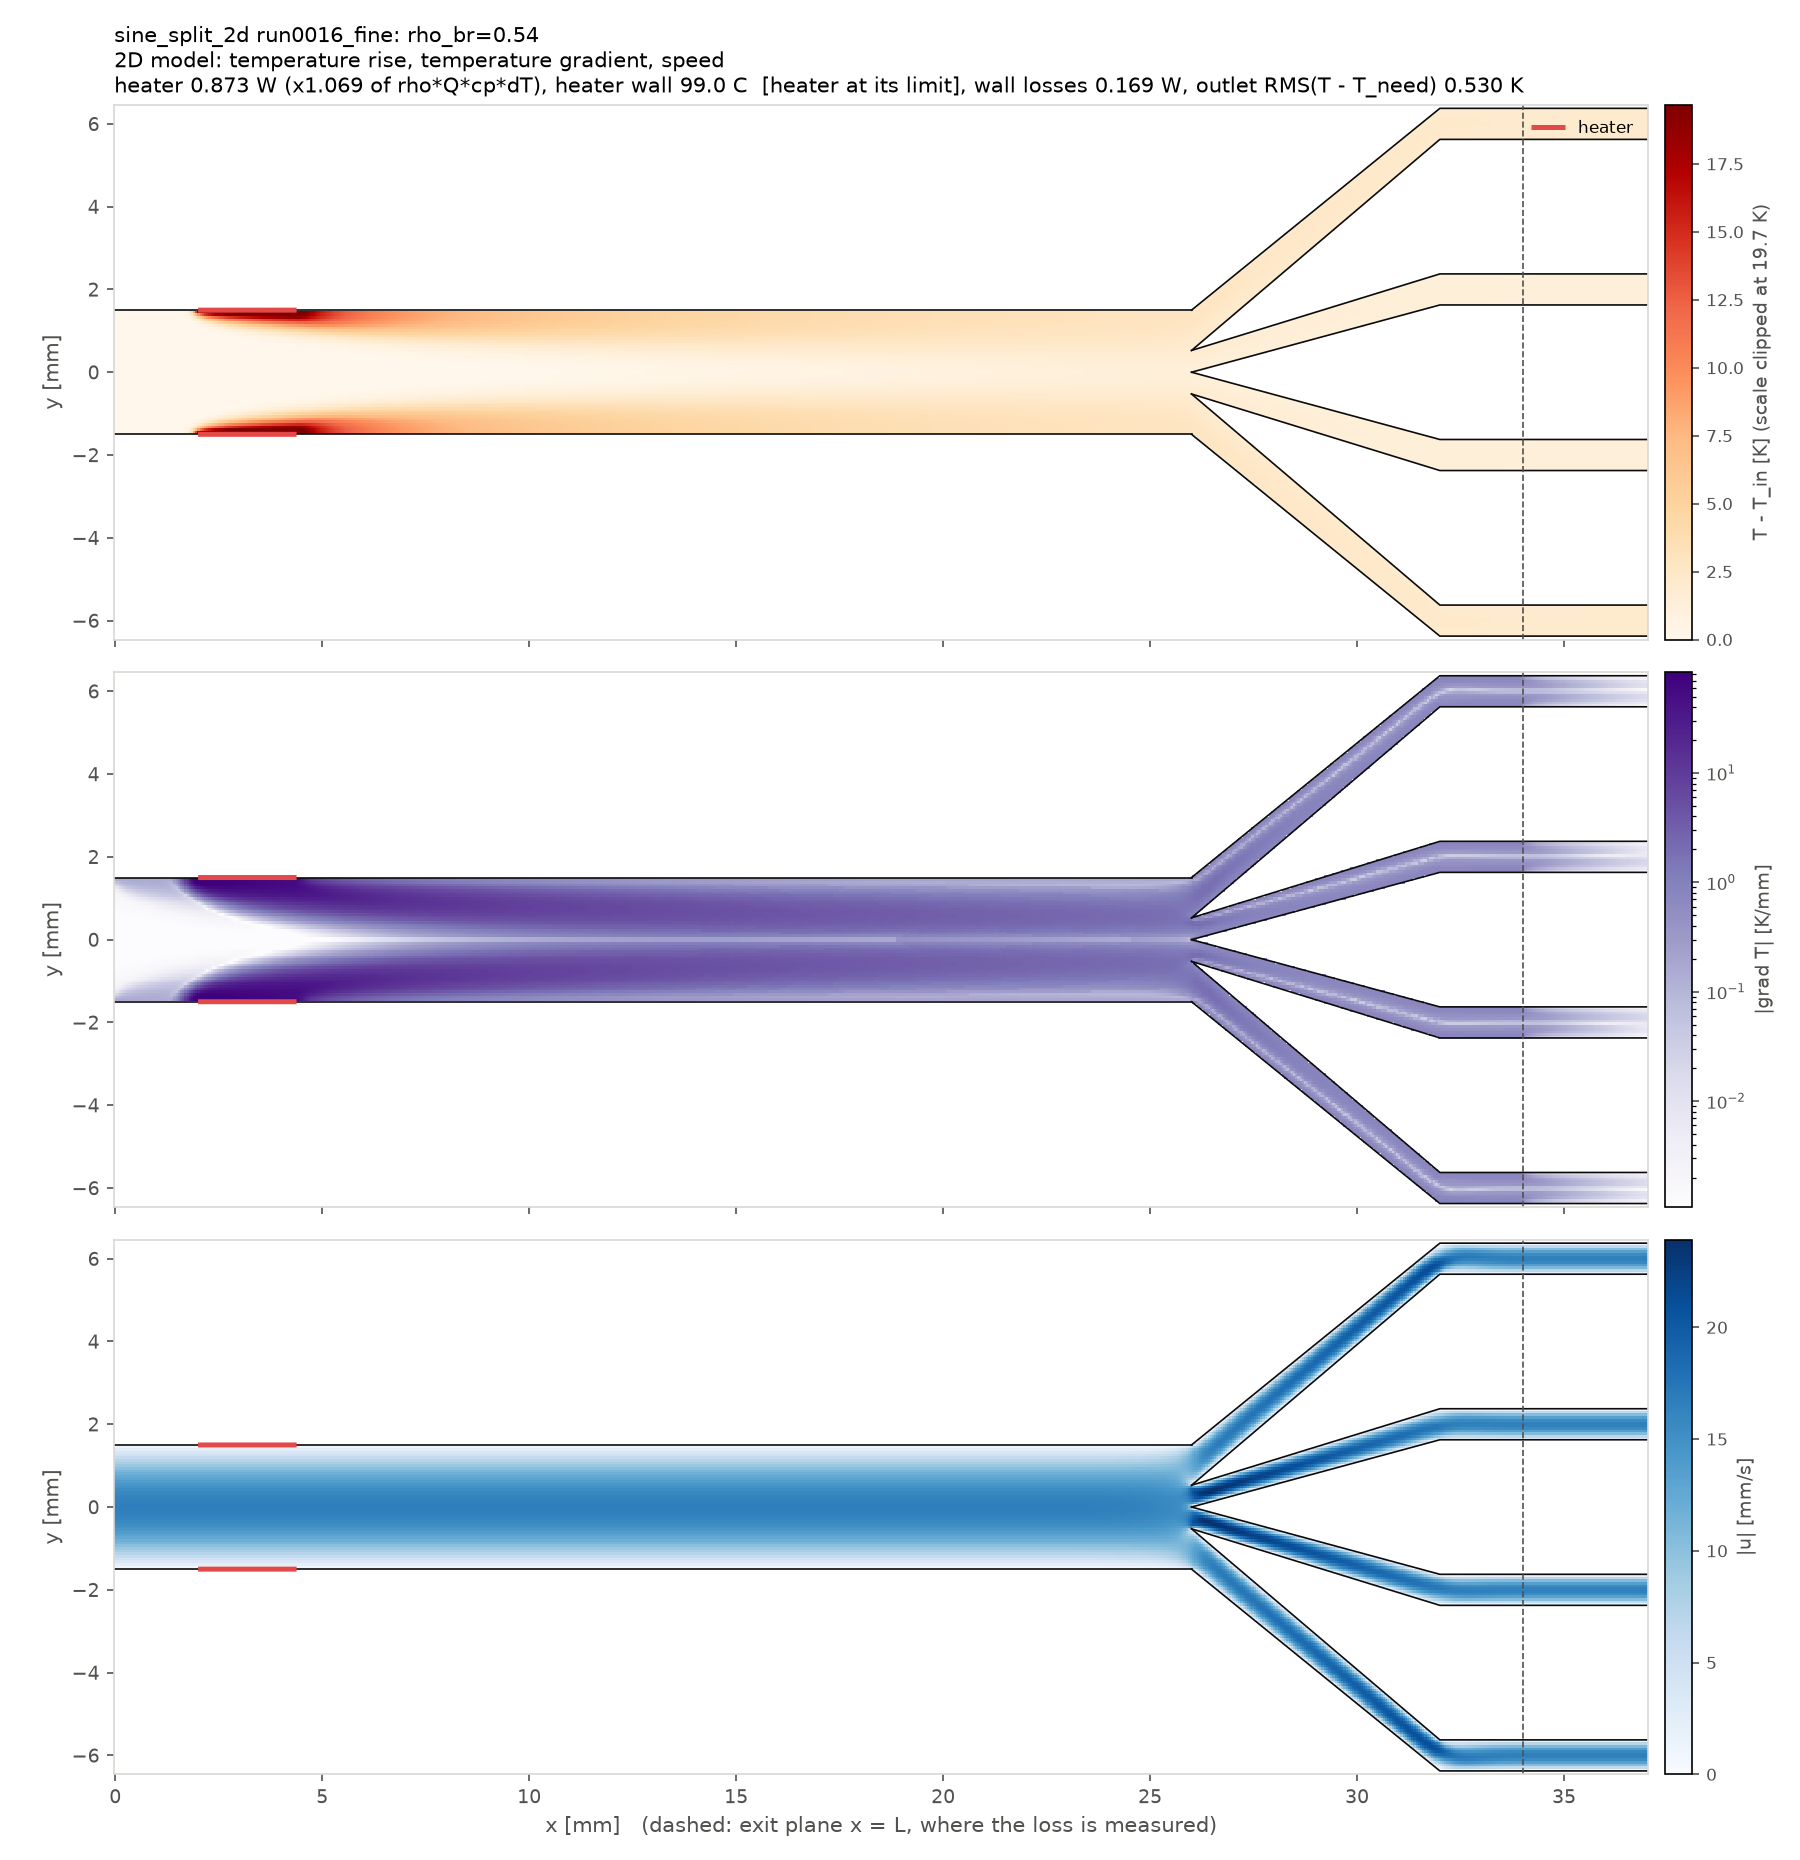
\includegraphics[width=0.95\textwidth,height=0.8\textheight,keepaspectratio]{runs/final_b2d_straight_maps.png}
\caption{Temperature rise, temperature gradient and speed (mid-depth plane in 3D). Red: heated wall. The title's ``outlet RMS'' is the area-weighted $\ell_{2,\mathrm{area}}$.}
\end{figure}
\begin{figure}[H]\centering
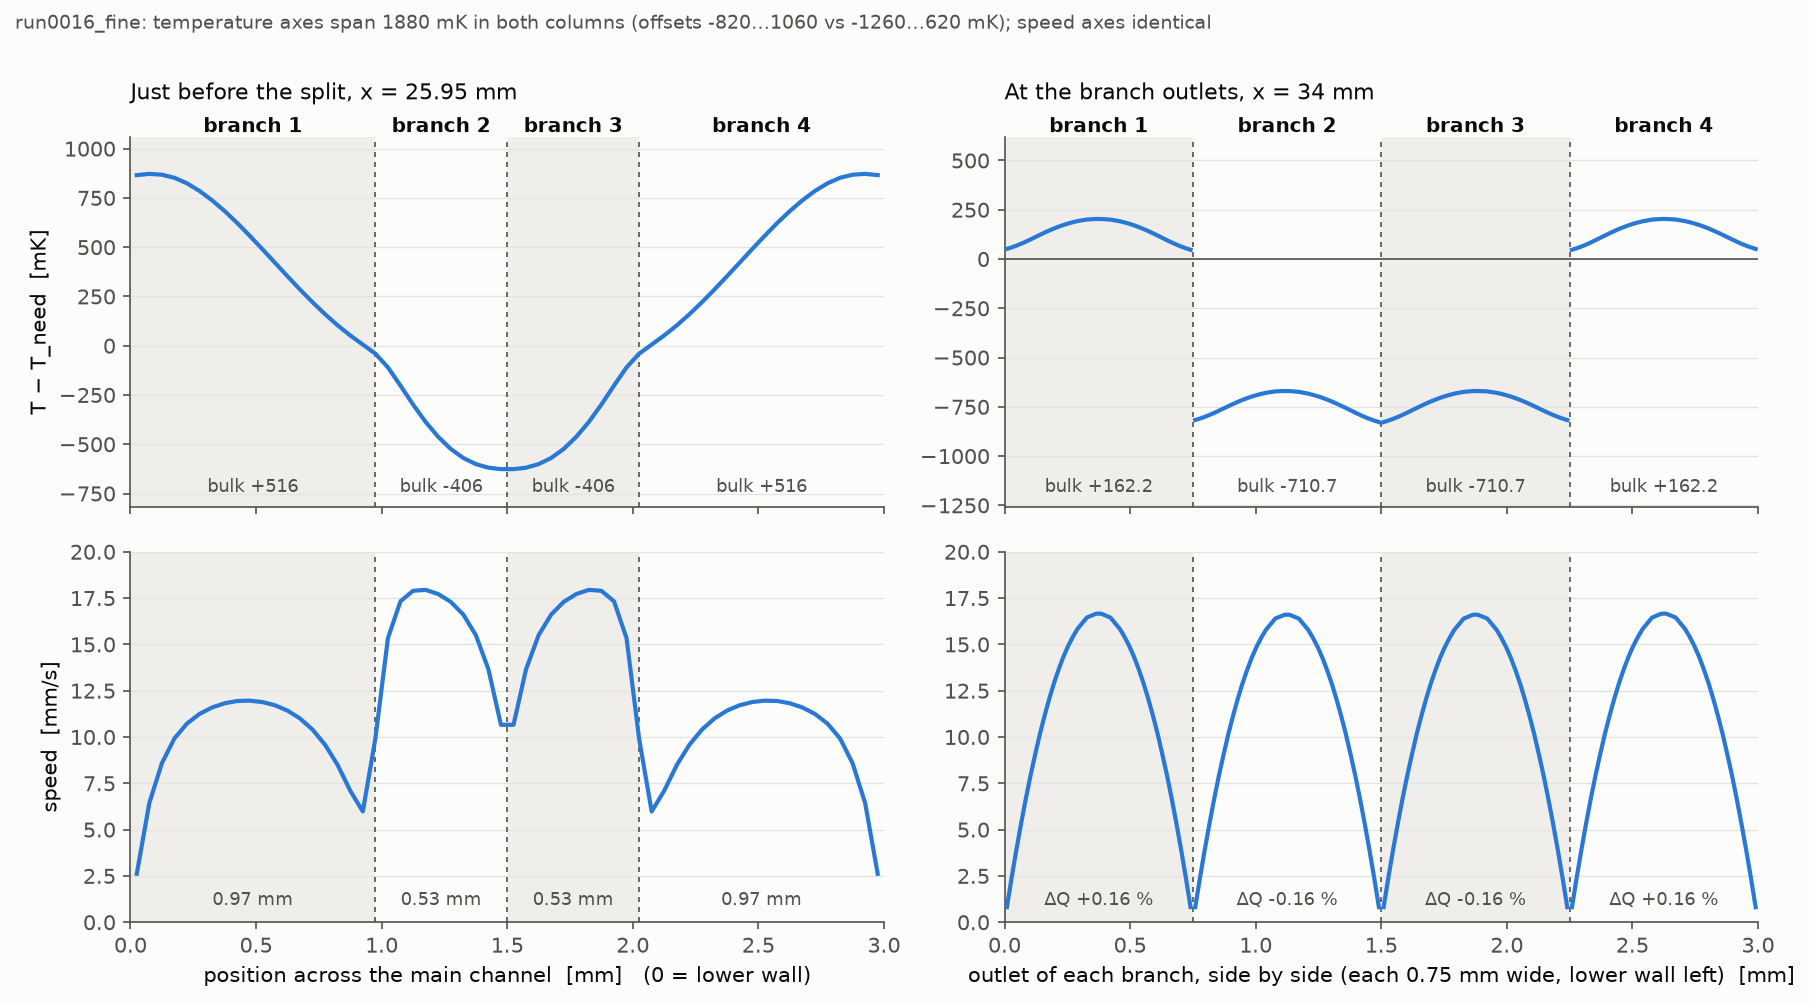
\includegraphics[width=0.95\textwidth,height=0.8\textheight,keepaspectratio]{runs/final_b2d_straight_presplit.png}
\caption{Cross-section just before the split, cut into the four branch inlets, next to each branch outlet.}
\end{figure}
\begin{figure}[H]\centering
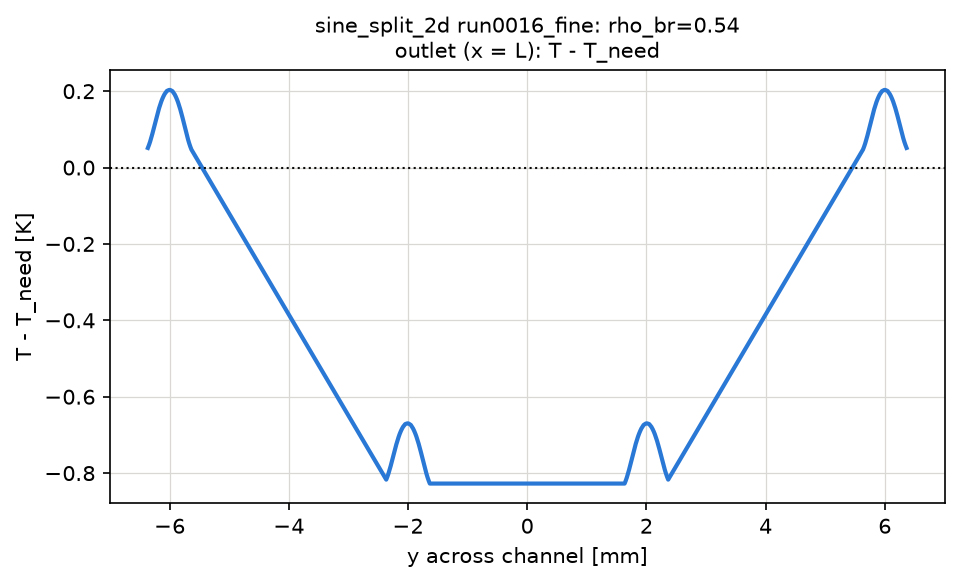
\includegraphics[width=0.75\textwidth,height=0.8\textheight,keepaspectratio]{runs/final_b2d_straight_outlet.png}
\caption{Outlet temperature (and, in 3D, the outlet plane).}
\end{figure}
\begin{figure}[H]\centering
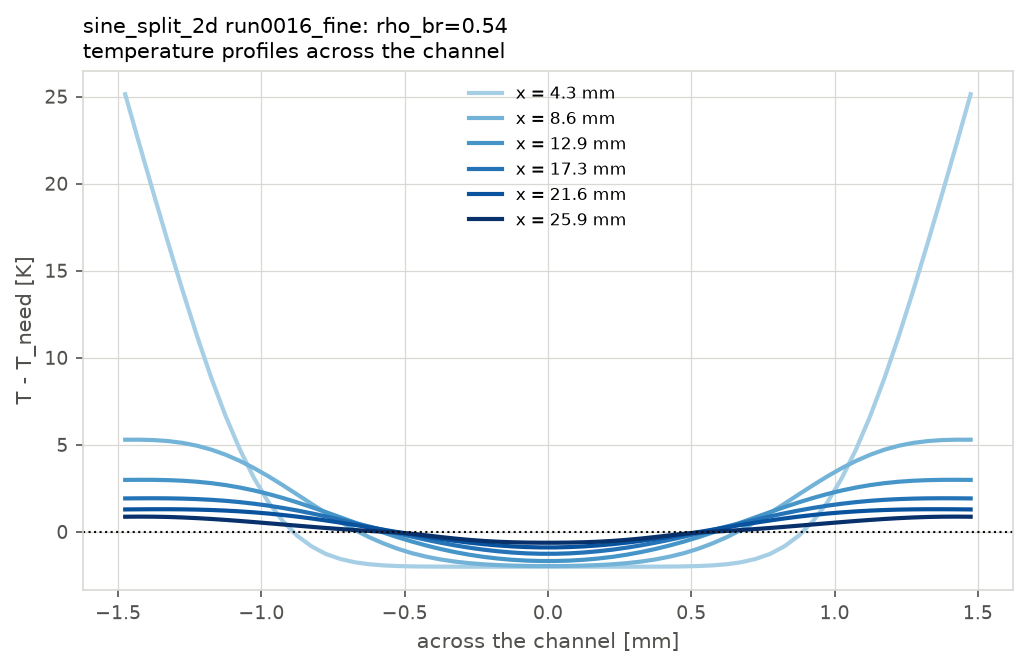
\includegraphics[width=0.62\textwidth,height=0.8\textheight,keepaspectratio]{runs/final_b2d_straight_slices.png}
\caption{Temperature profiles across the channel at several $x$ stations.}
\end{figure}
\begin{figure}[H]\centering
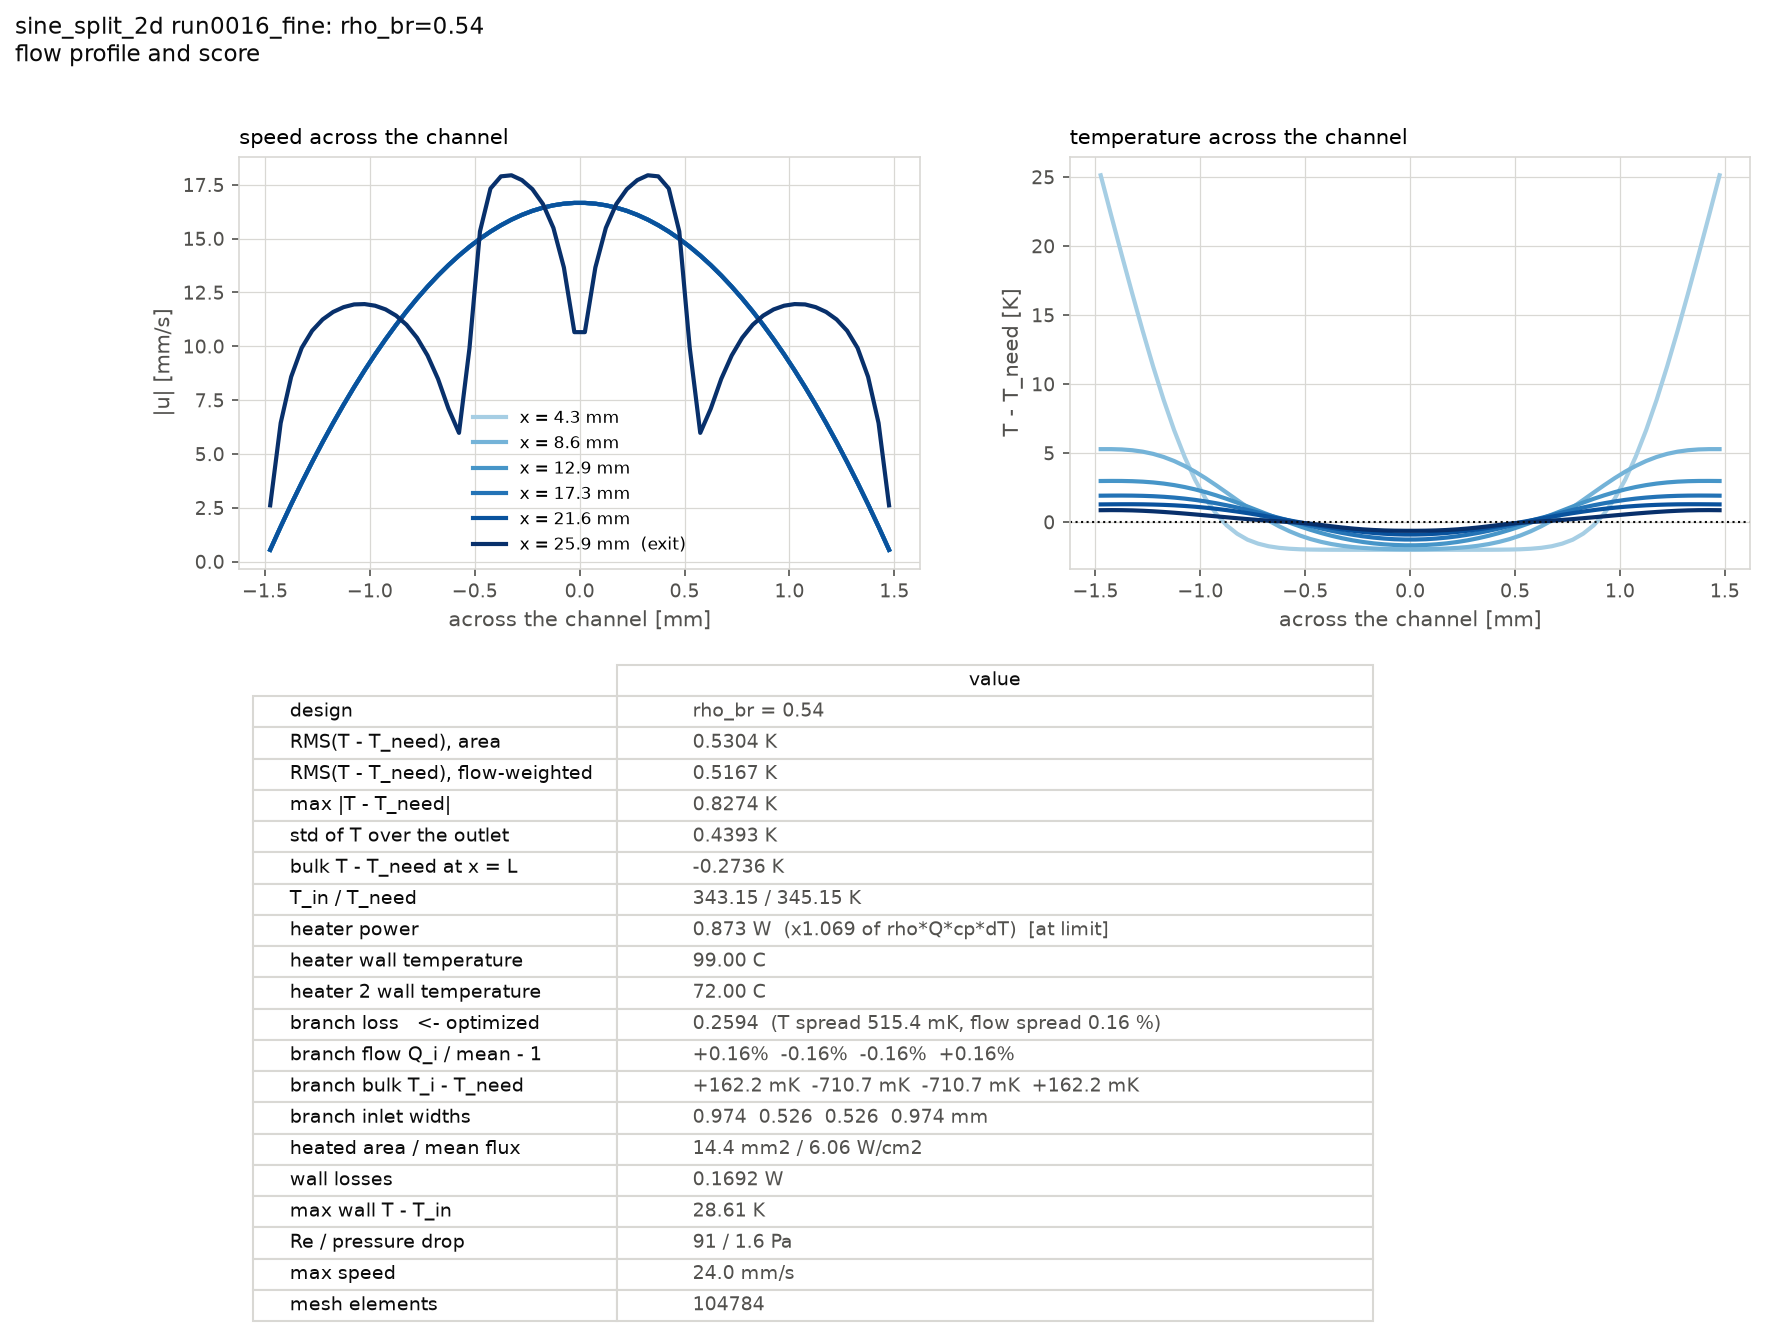
\includegraphics[width=0.8\textwidth,height=0.8\textheight,keepaspectratio]{runs/final_b2d_straight_profile.png}
\caption{Speed and temperature across the channel at several $x$ stations, and the full score table of the design.}
\end{figure}
\begin{figure}[H]\centering
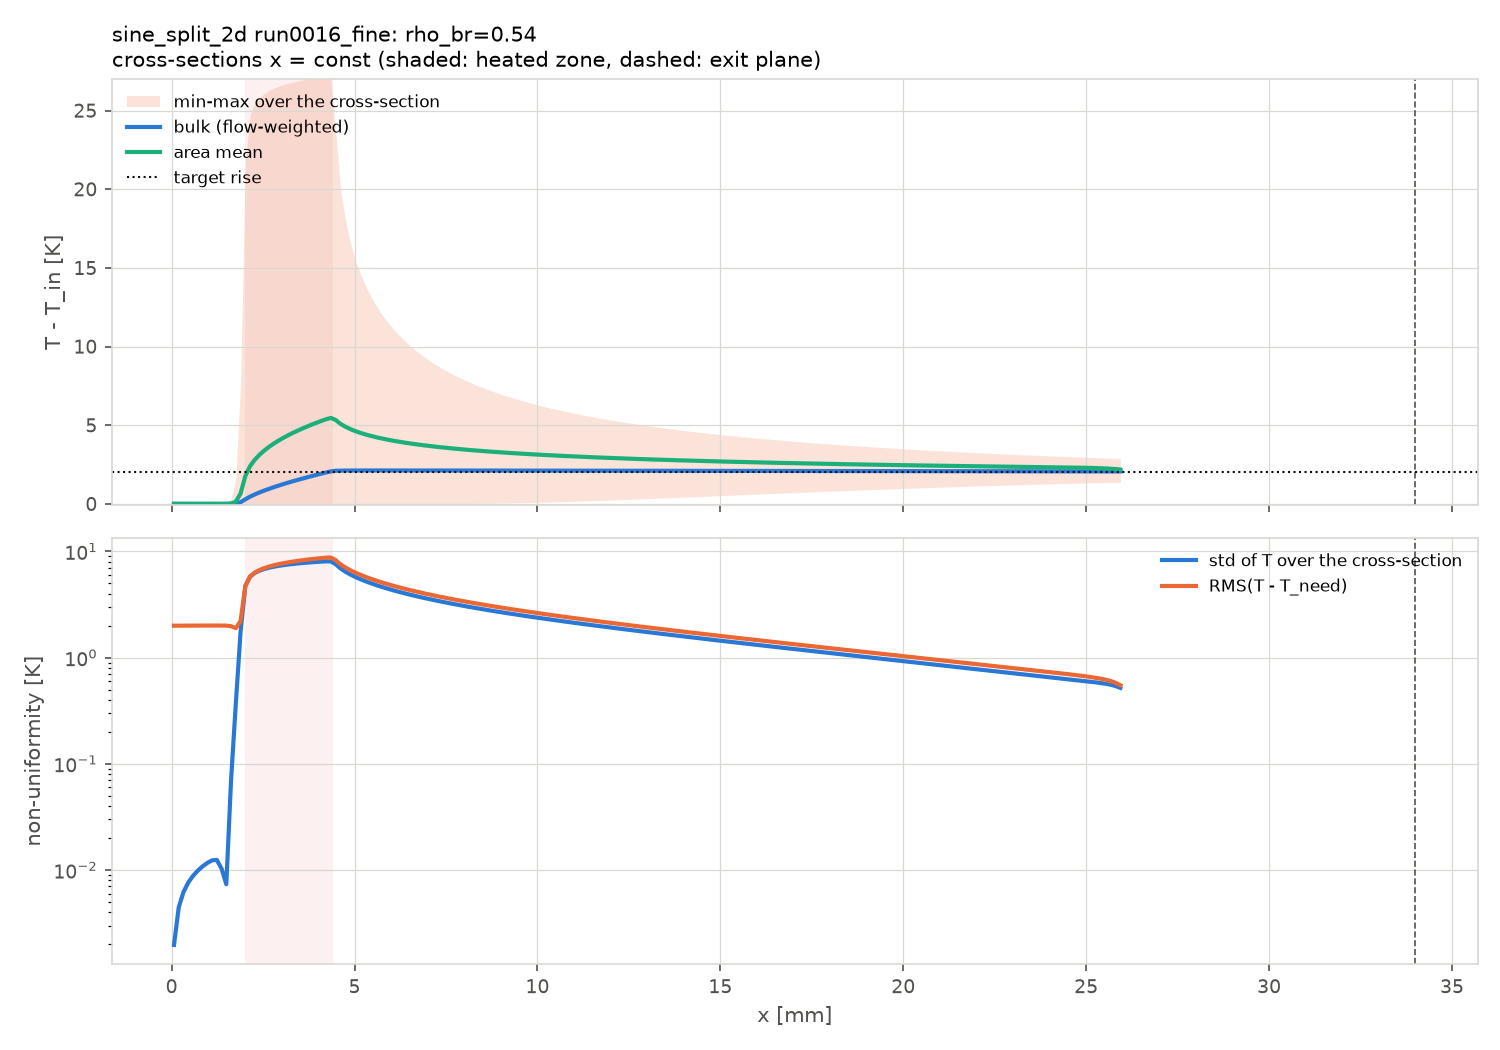
\includegraphics[width=0.8\textwidth,height=0.8\textheight,keepaspectratio]{runs/final_b2d_straight_along_x.png}
\caption{Bulk, mean, min and max temperature along the channel.}
\end{figure}
\begin{figure}[H]\centering
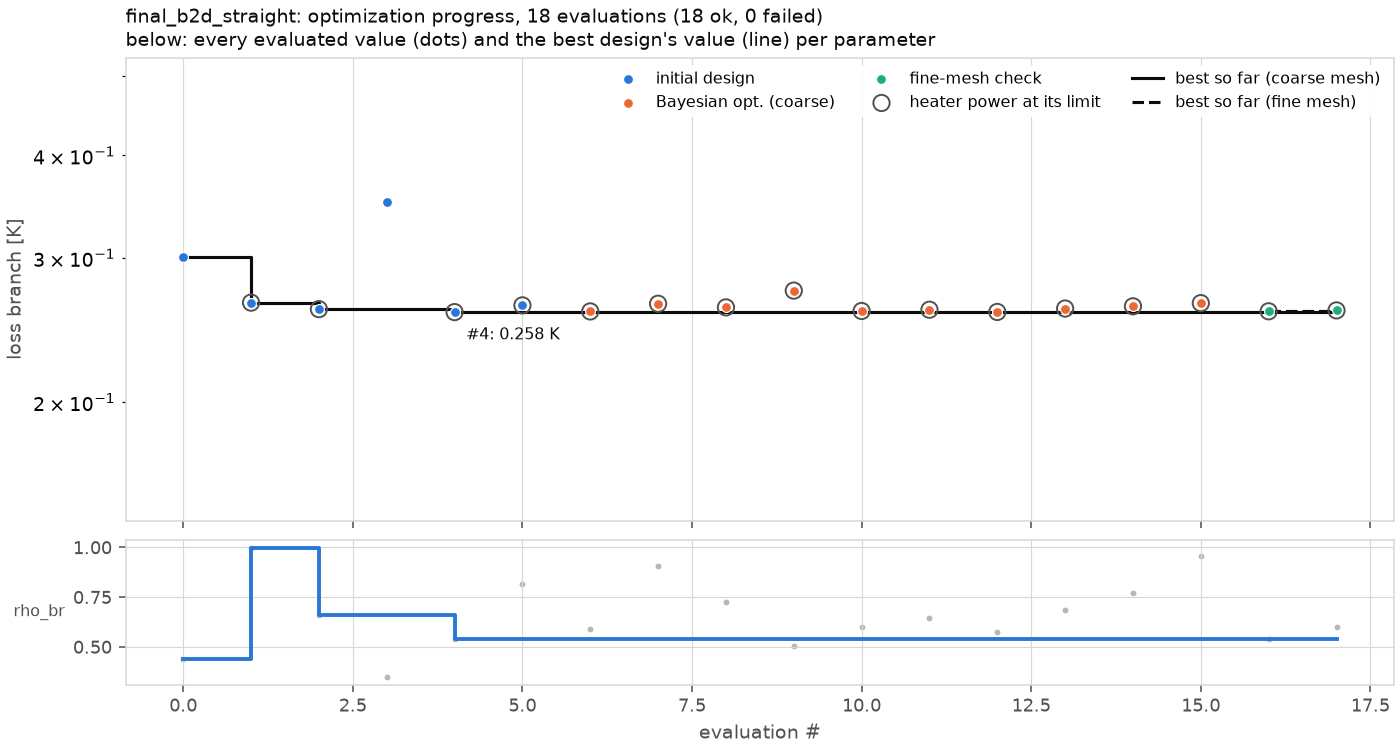
\includegraphics[width=0.85\textwidth]{runs/final_b2d_straight_progress_loss.png}
\caption{Search history: loss of every evaluation, best so far, and the parameters.}
\end{figure}
\clearpage
\subsubsection*{Branched sine + straight, BO best \#150: 116\mK, 0.82\,\%}
\noindent\texttt{runs/final\_b2d\_sine}\par\medskip
\begin{figure}[H]\centering
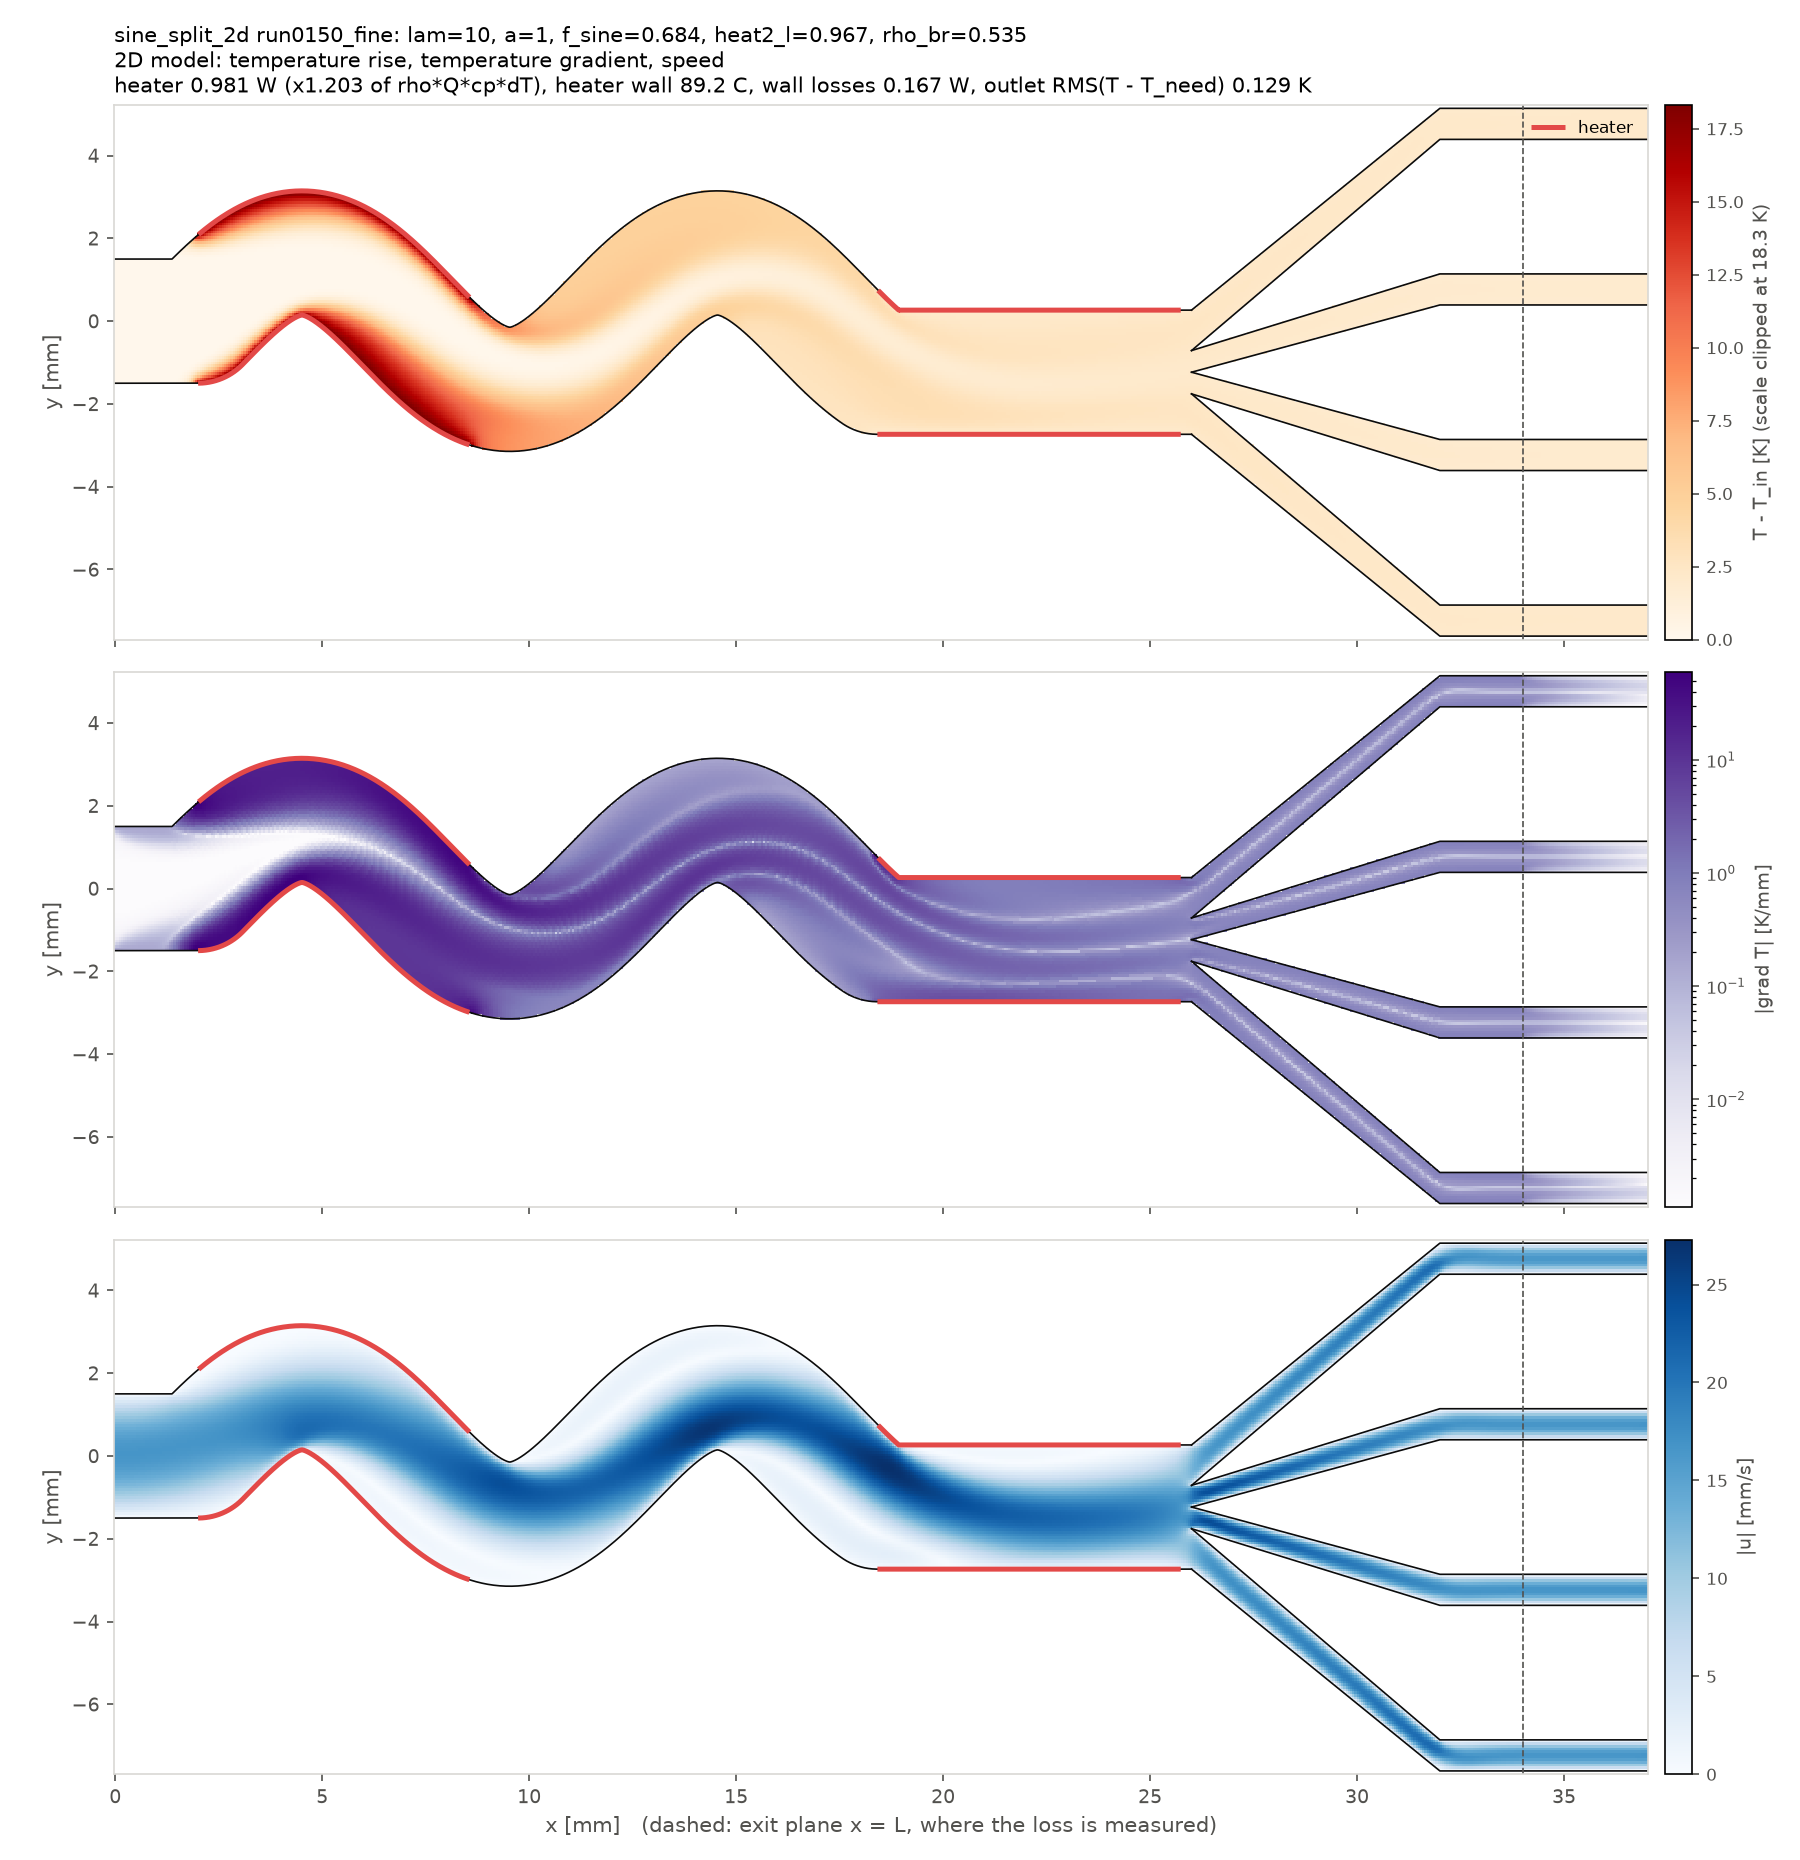
\includegraphics[width=0.95\textwidth,height=0.8\textheight,keepaspectratio]{runs/final_b2d_sine_maps.png}
\caption{Temperature rise, temperature gradient and speed (mid-depth plane in 3D). Red: heated wall. The title's ``outlet RMS'' is the area-weighted $\ell_{2,\mathrm{area}}$.}
\end{figure}
\begin{figure}[H]\centering
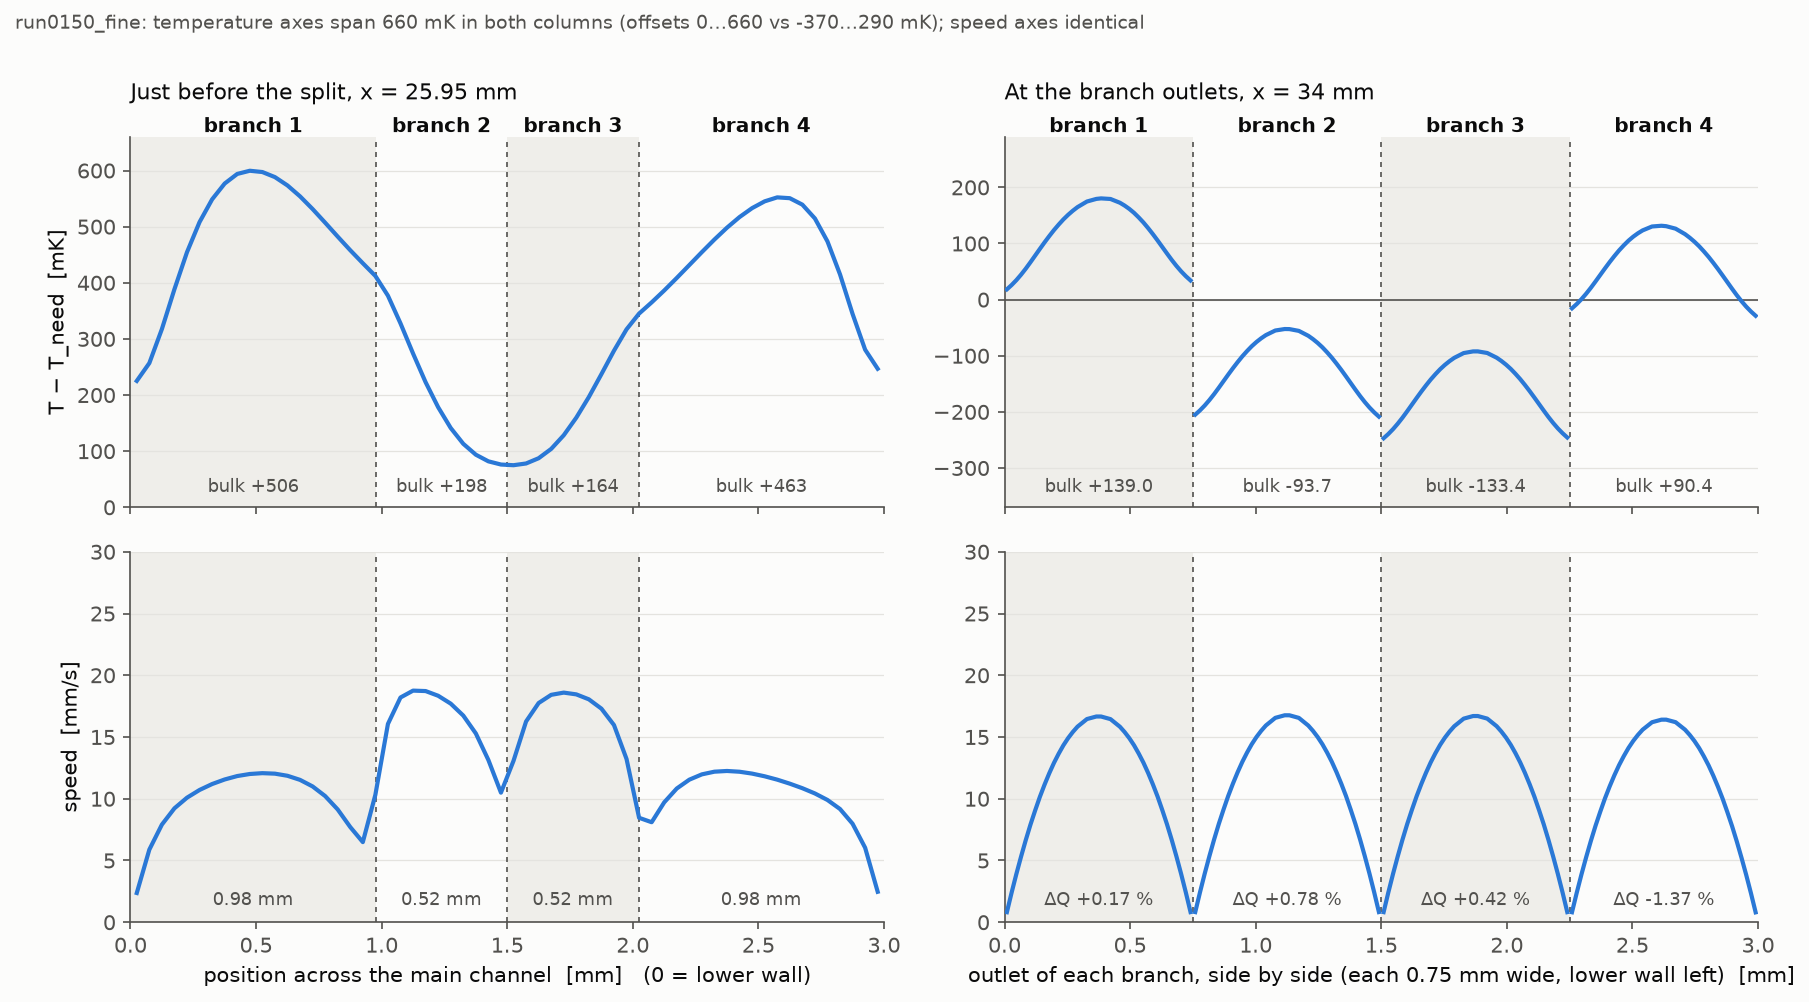
\includegraphics[width=0.95\textwidth,height=0.8\textheight,keepaspectratio]{runs/final_b2d_sine_presplit.png}
\caption{Cross-section just before the split, cut into the four branch inlets, next to each branch outlet.}
\end{figure}
\begin{figure}[H]\centering
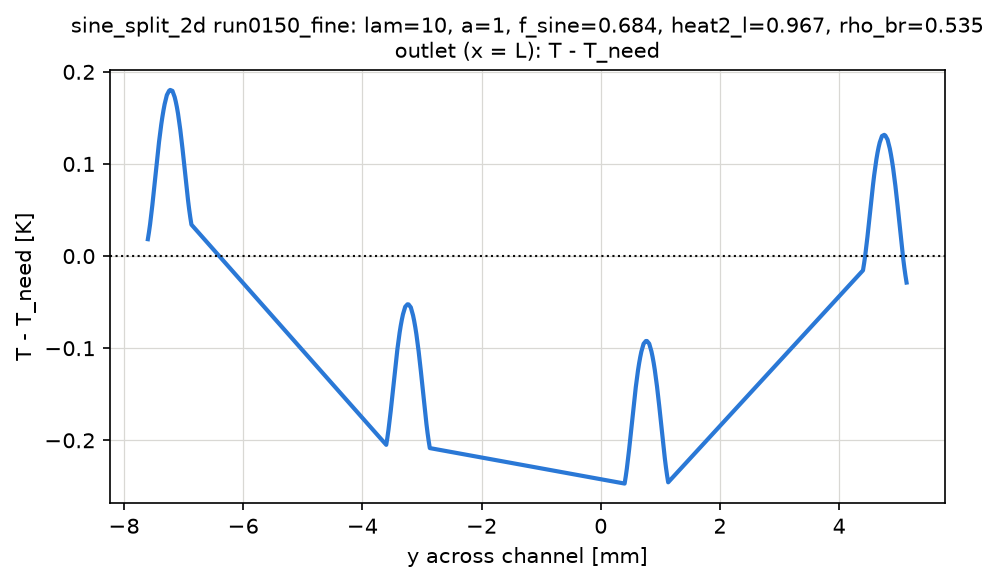
\includegraphics[width=0.75\textwidth,height=0.8\textheight,keepaspectratio]{runs/final_b2d_sine_outlet.png}
\caption{Outlet temperature (and, in 3D, the outlet plane).}
\end{figure}
\begin{figure}[H]\centering
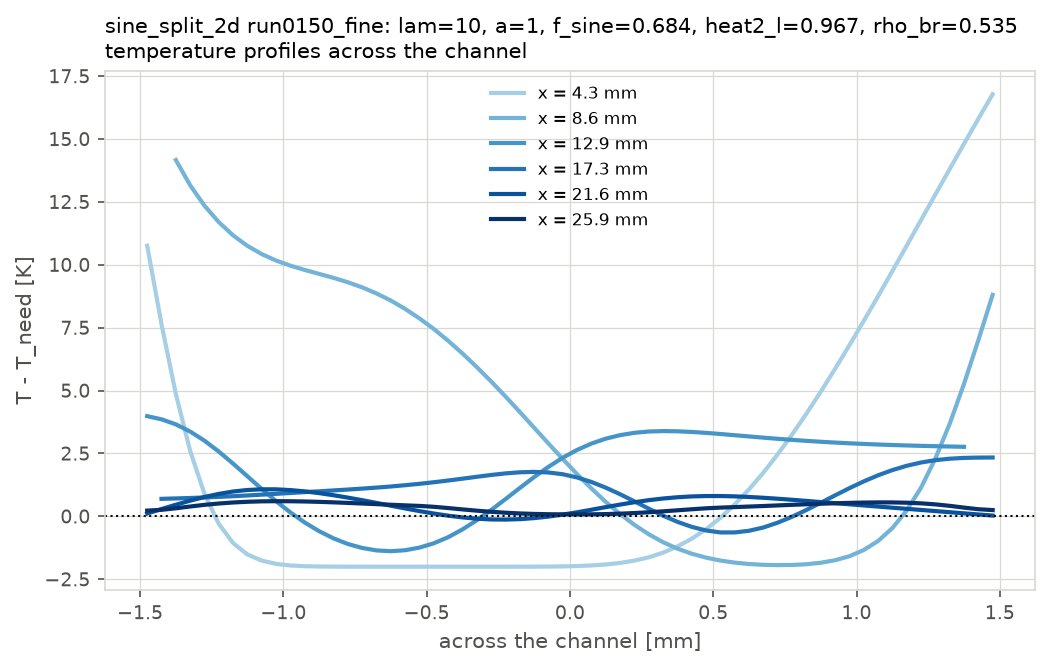
\includegraphics[width=0.62\textwidth,height=0.8\textheight,keepaspectratio]{runs/final_b2d_sine_slices.png}
\caption{Temperature profiles across the channel at several $x$ stations.}
\end{figure}
\begin{figure}[H]\centering
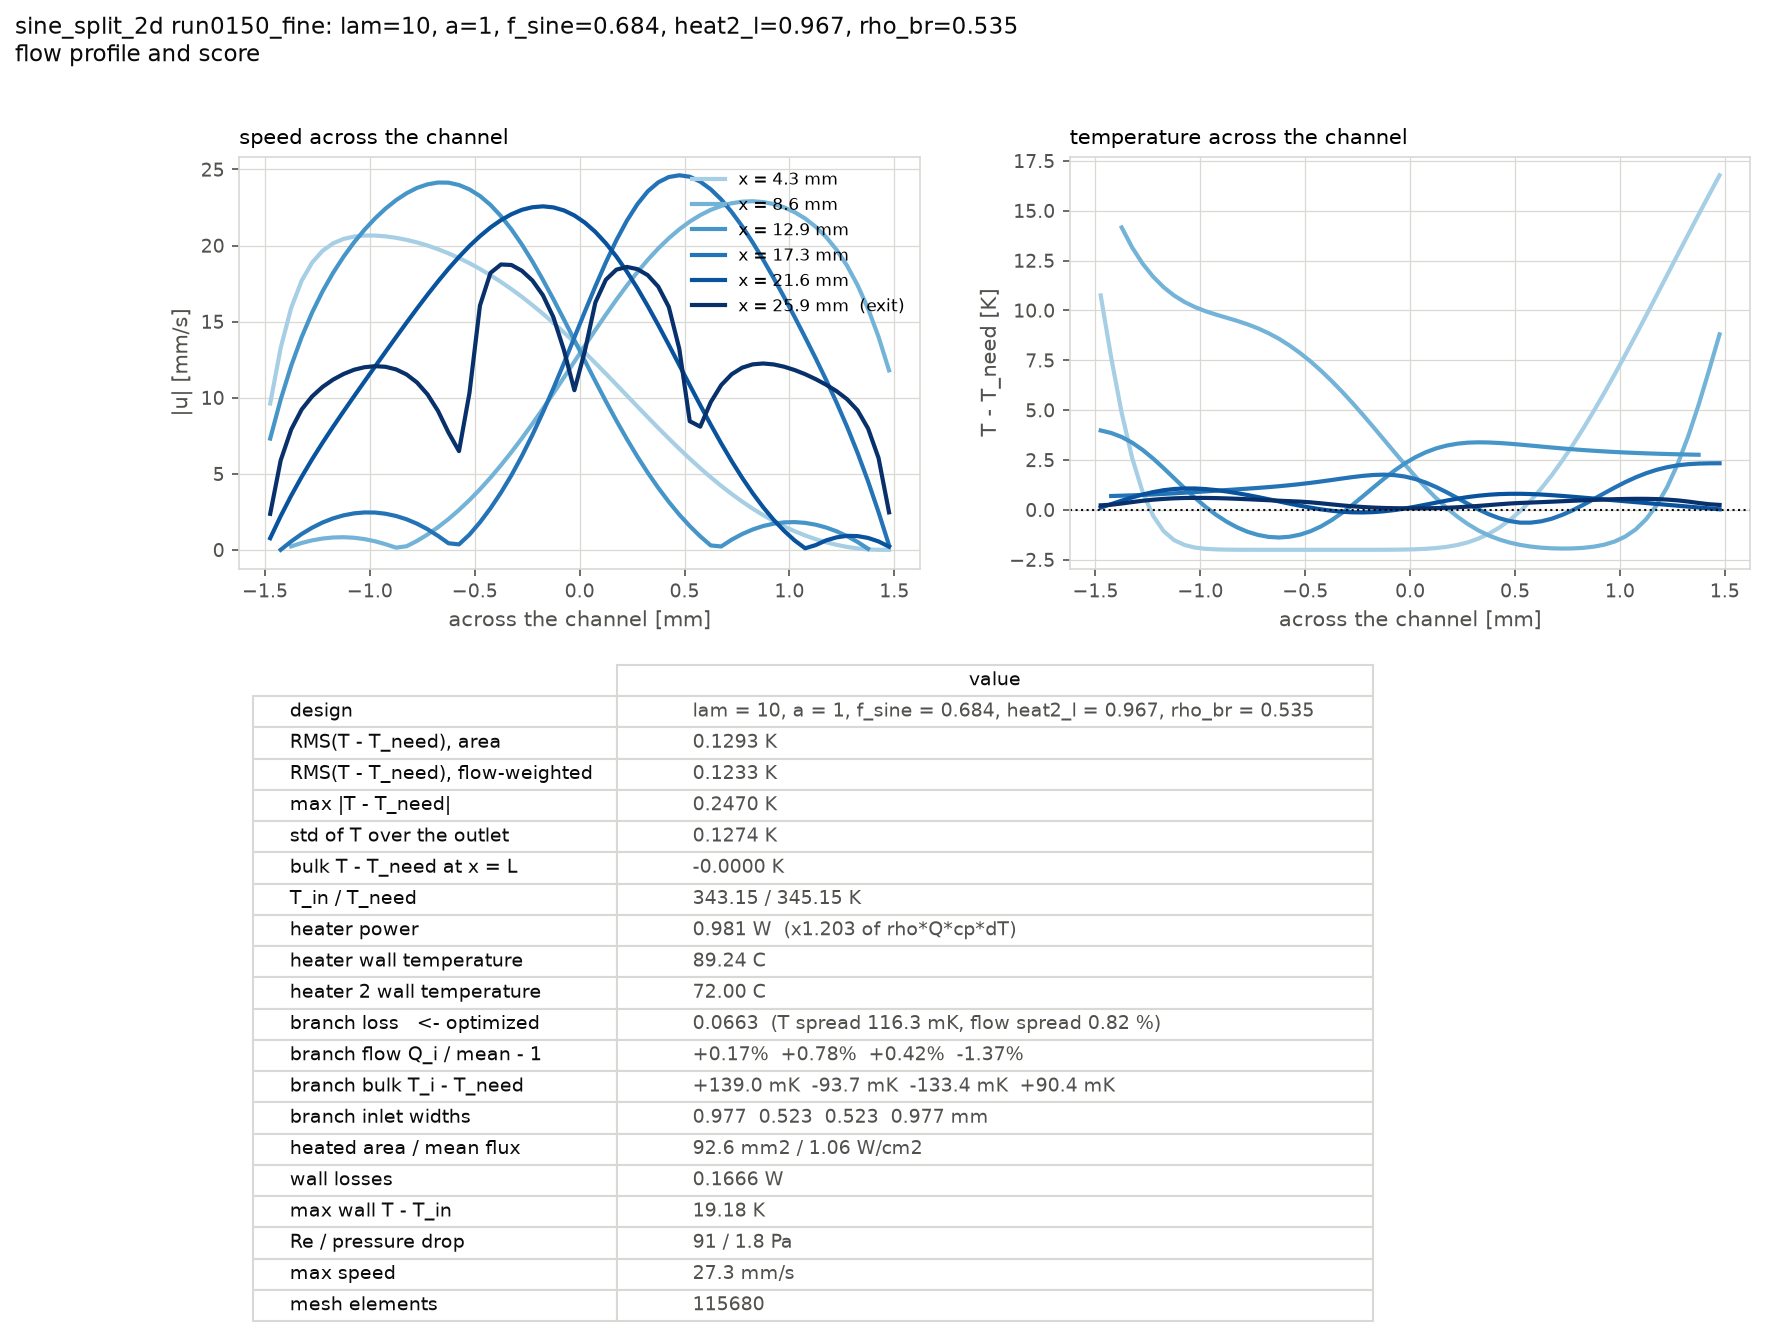
\includegraphics[width=0.8\textwidth,height=0.8\textheight,keepaspectratio]{runs/final_b2d_sine_profile.png}
\caption{Speed and temperature across the channel at several $x$ stations, and the full score table of the design.}
\end{figure}
\begin{figure}[H]\centering
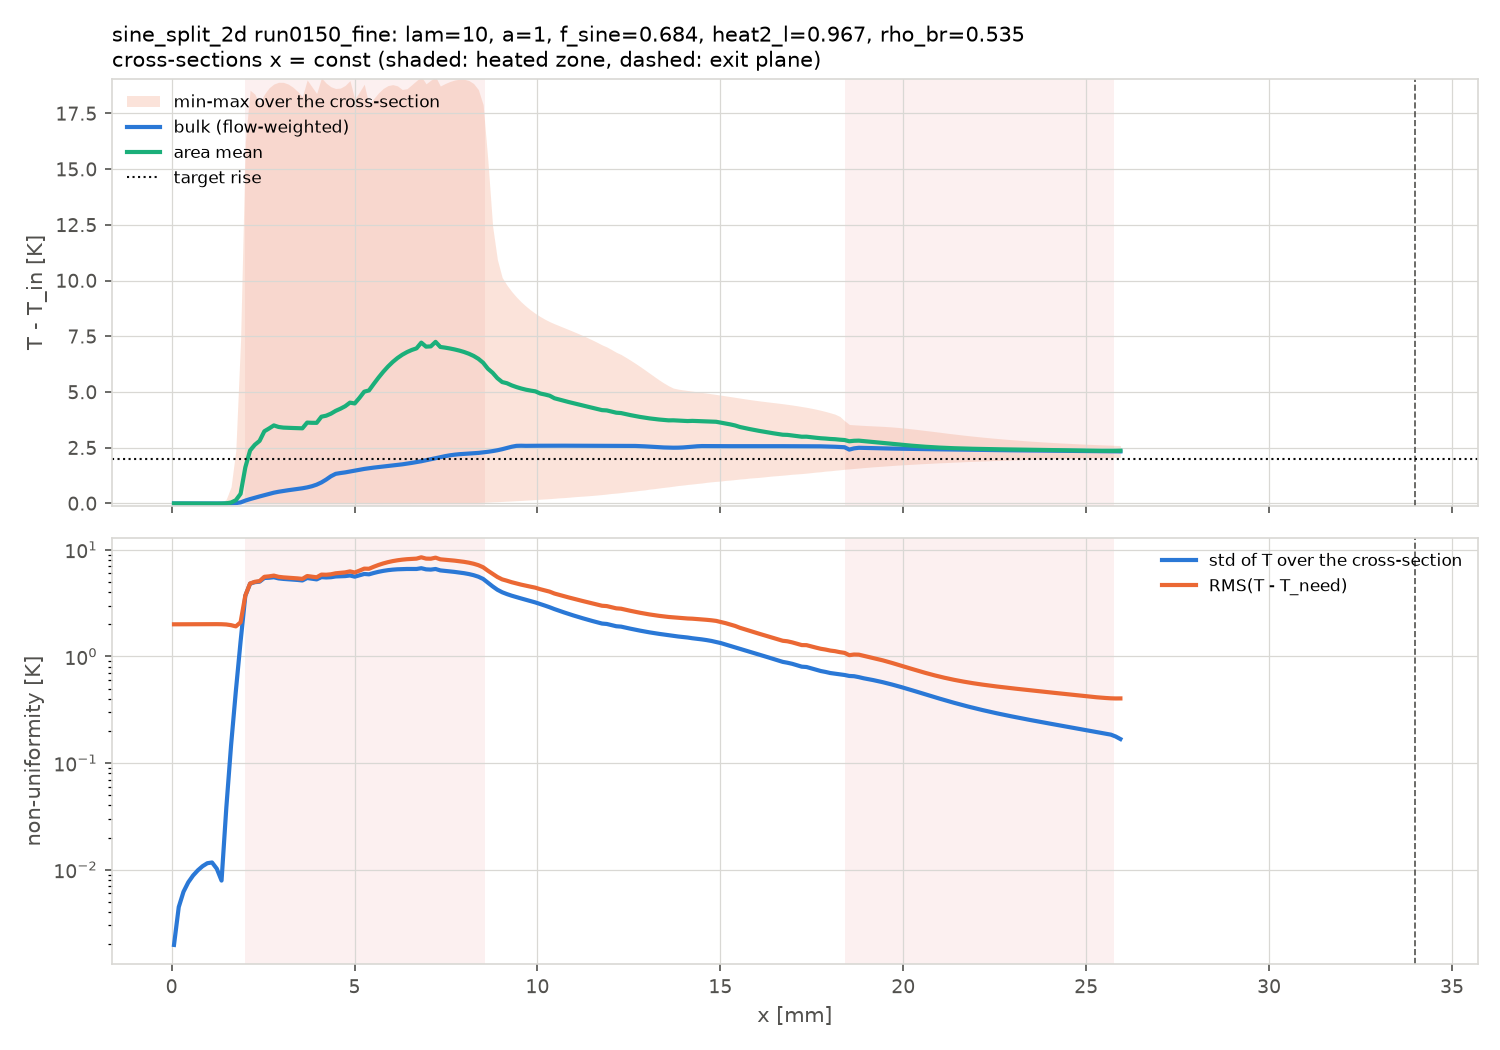
\includegraphics[width=0.8\textwidth,height=0.8\textheight,keepaspectratio]{runs/final_b2d_sine_along_x.png}
\caption{Bulk, mean, min and max temperature along the channel.}
\end{figure}
\begin{figure}[H]\centering
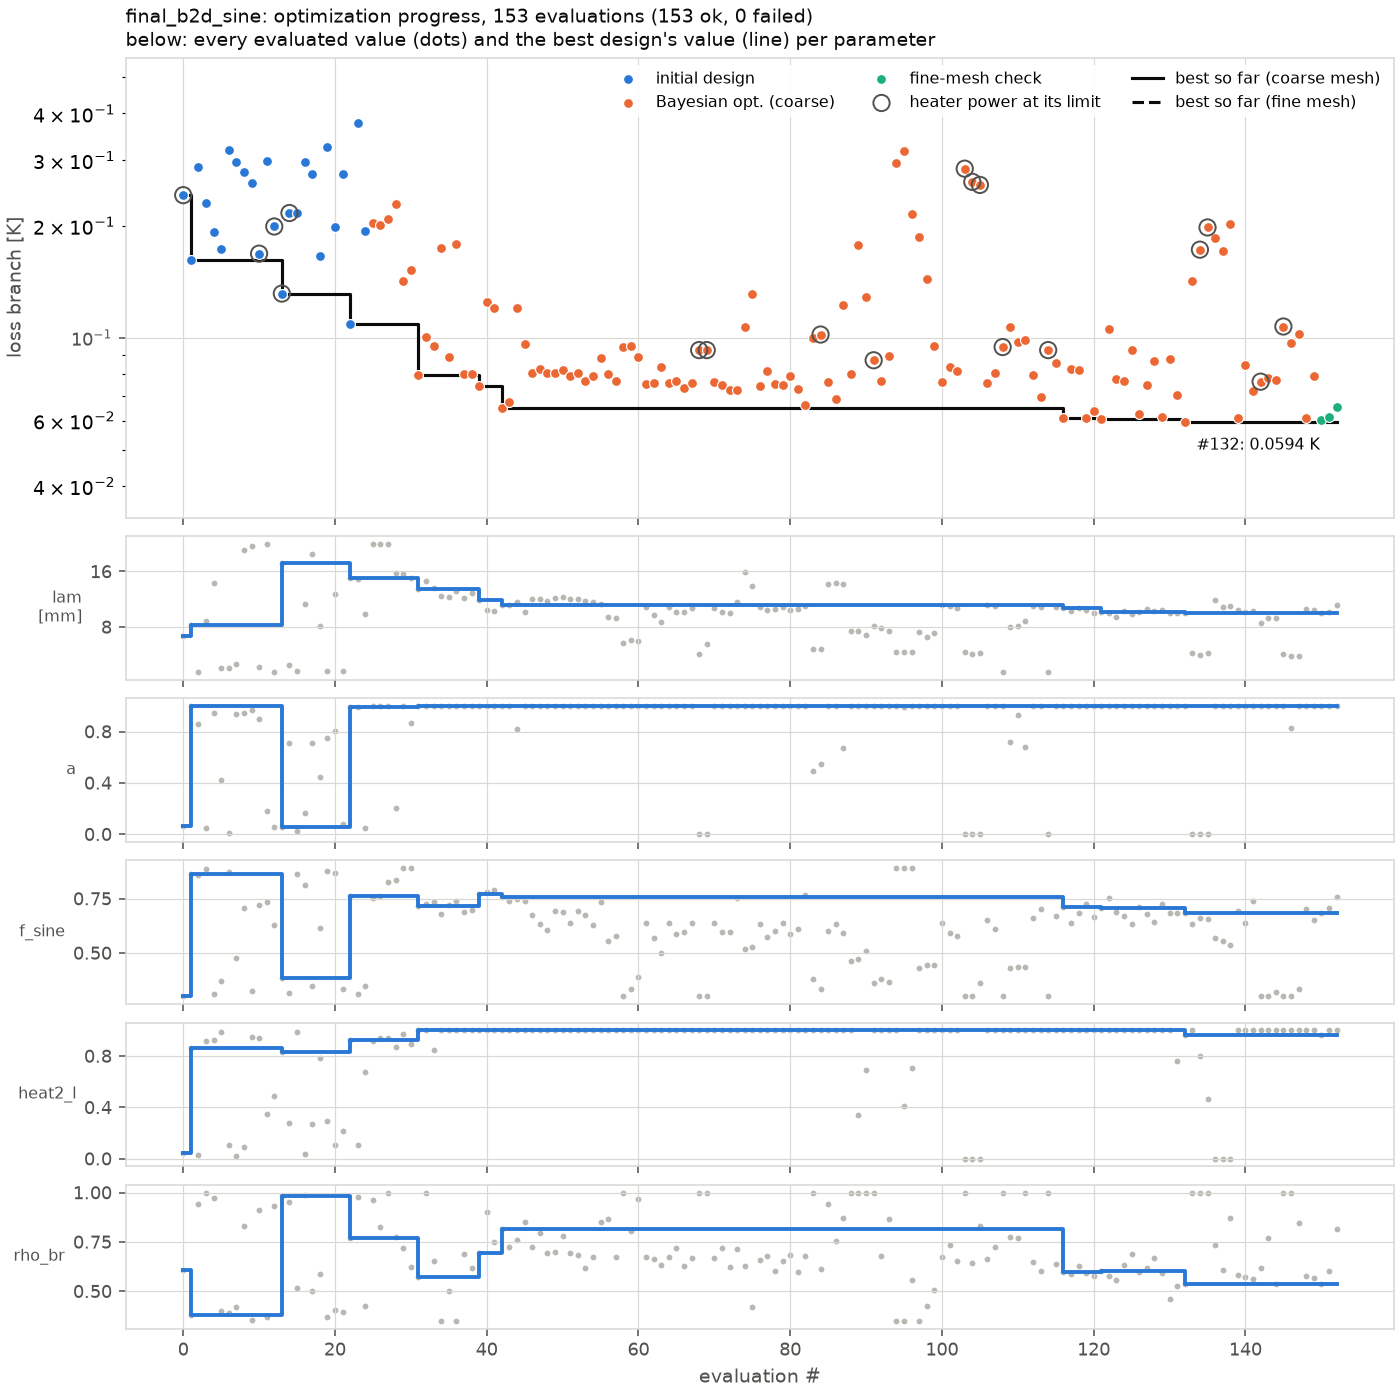
\includegraphics[width=0.85\textwidth]{runs/final_b2d_sine_progress_loss.png}
\caption{Search history: loss of every evaluation, best so far, and the parameters.}
\end{figure}
\clearpage
\subsubsection*{Branched serpentine + straight, BO best \#150: 12.3\mK, 3.9\,\%}
\noindent\texttt{runs/final\_b2d\_serp}\par\medskip
\begin{figure}[H]\centering
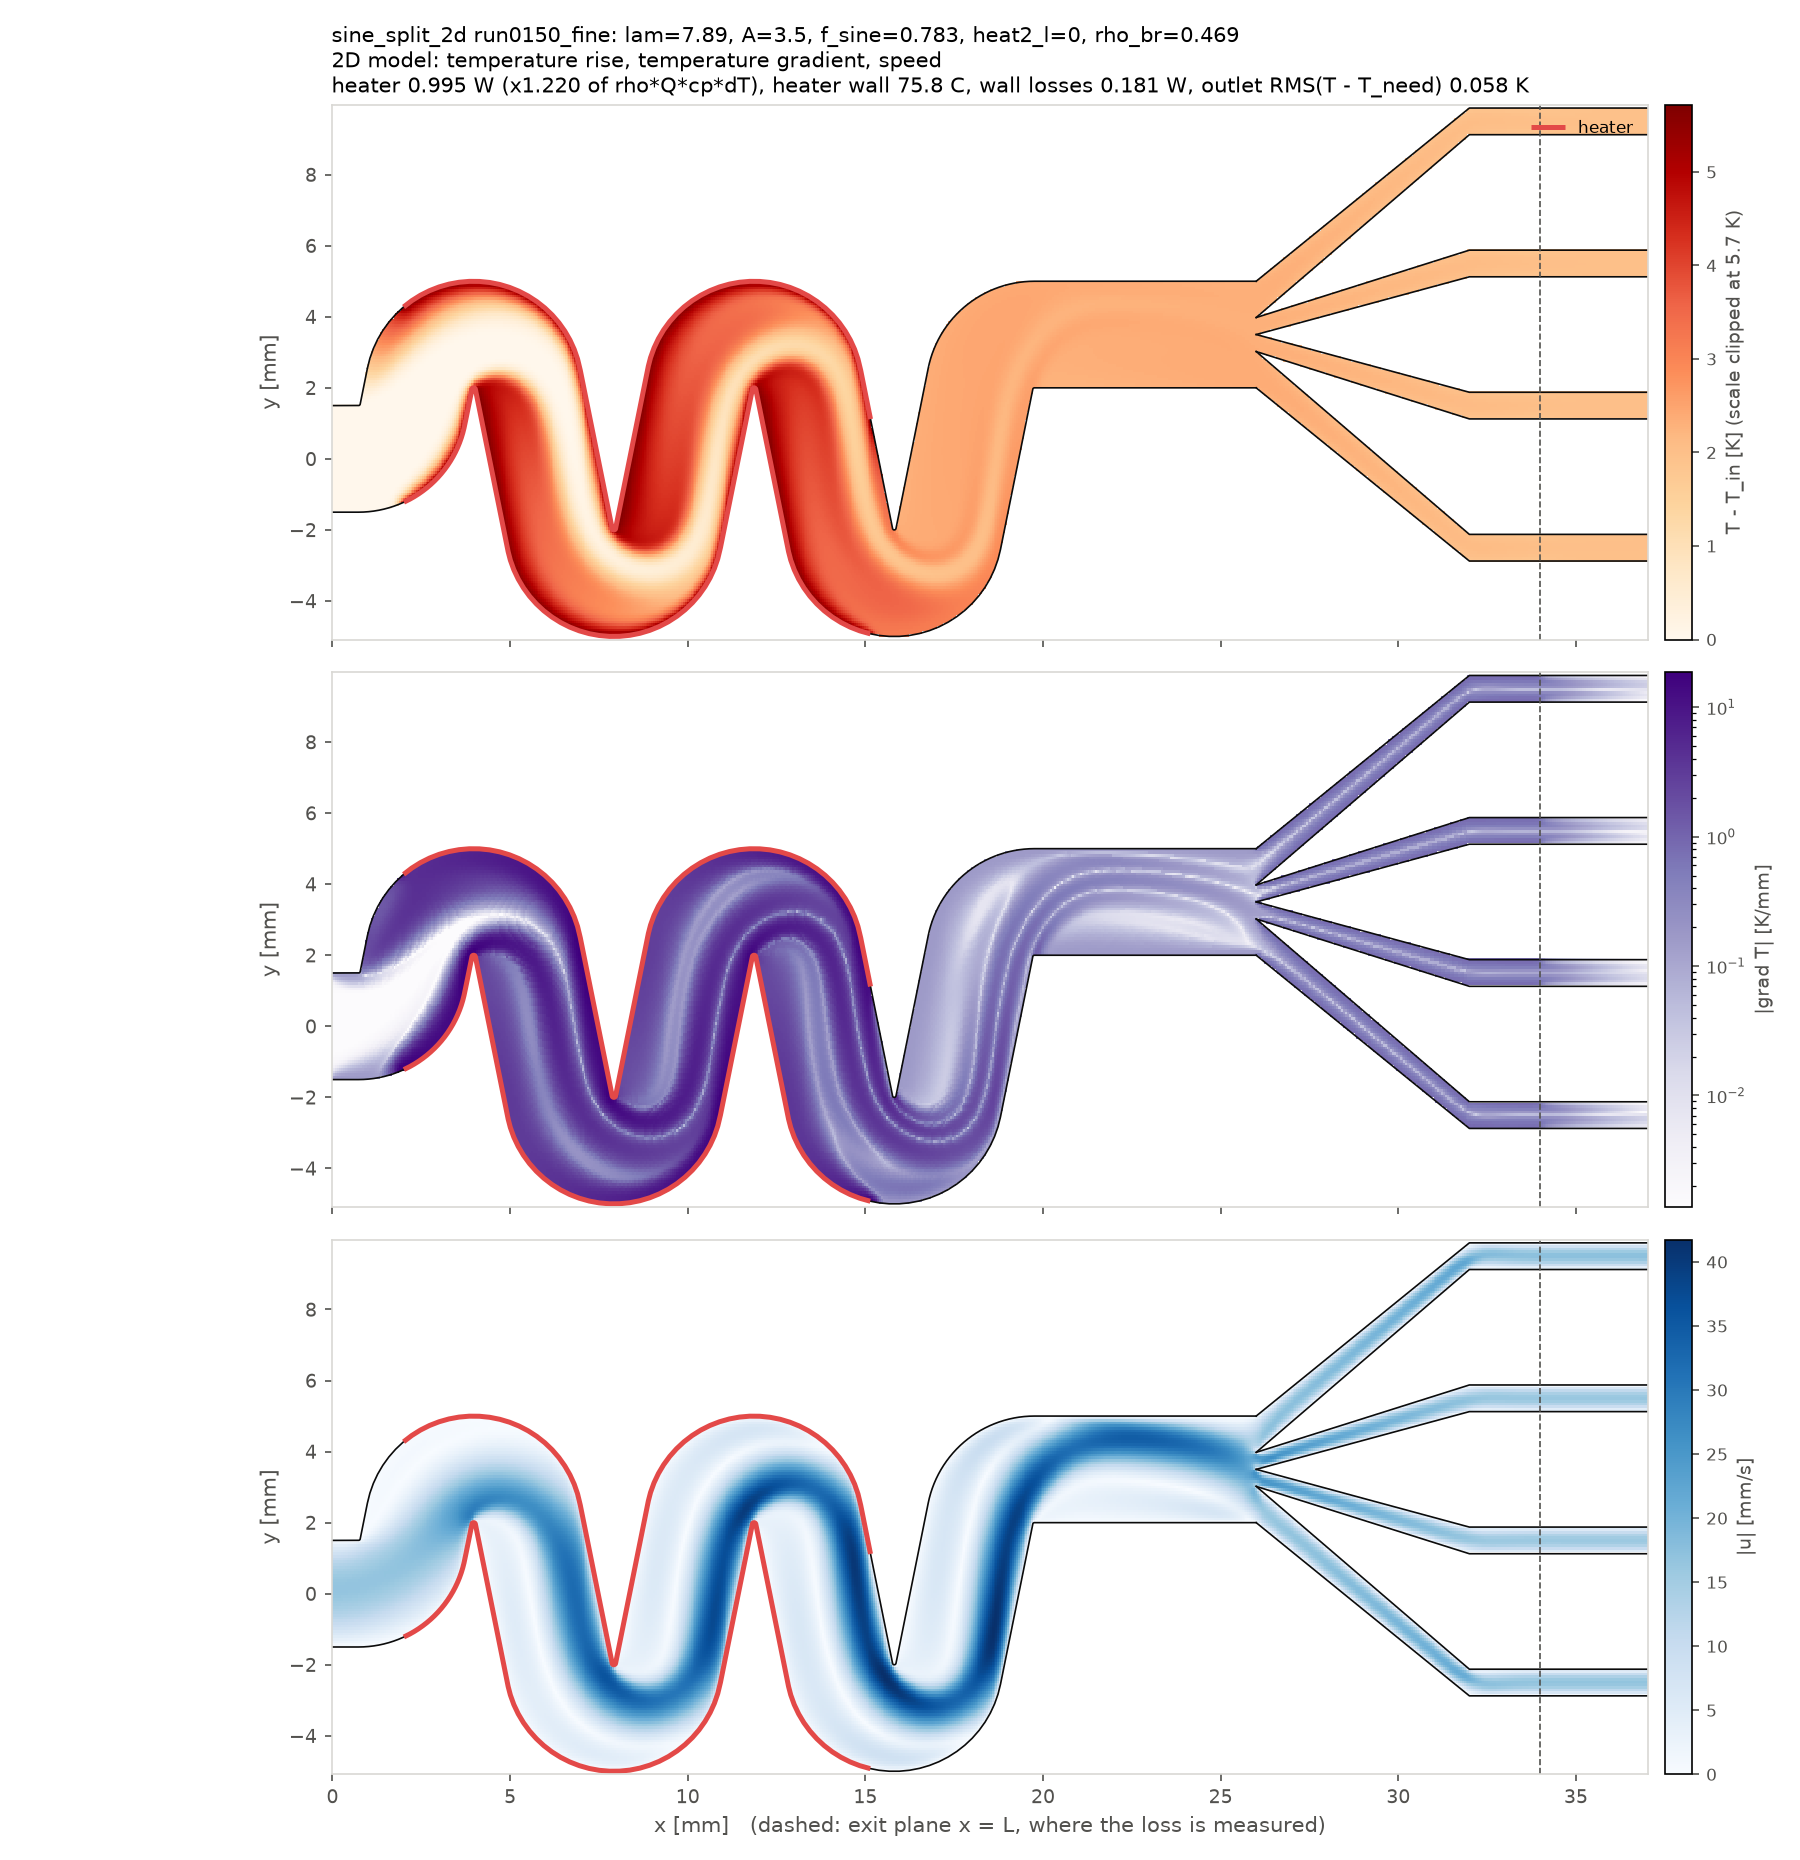
\includegraphics[width=0.95\textwidth,height=0.8\textheight,keepaspectratio]{runs/final_b2d_serp_maps.png}
\caption{Temperature rise, temperature gradient and speed (mid-depth plane in 3D). Red: heated wall. The title's ``outlet RMS'' is the area-weighted $\ell_{2,\mathrm{area}}$.}
\end{figure}
\begin{figure}[H]\centering
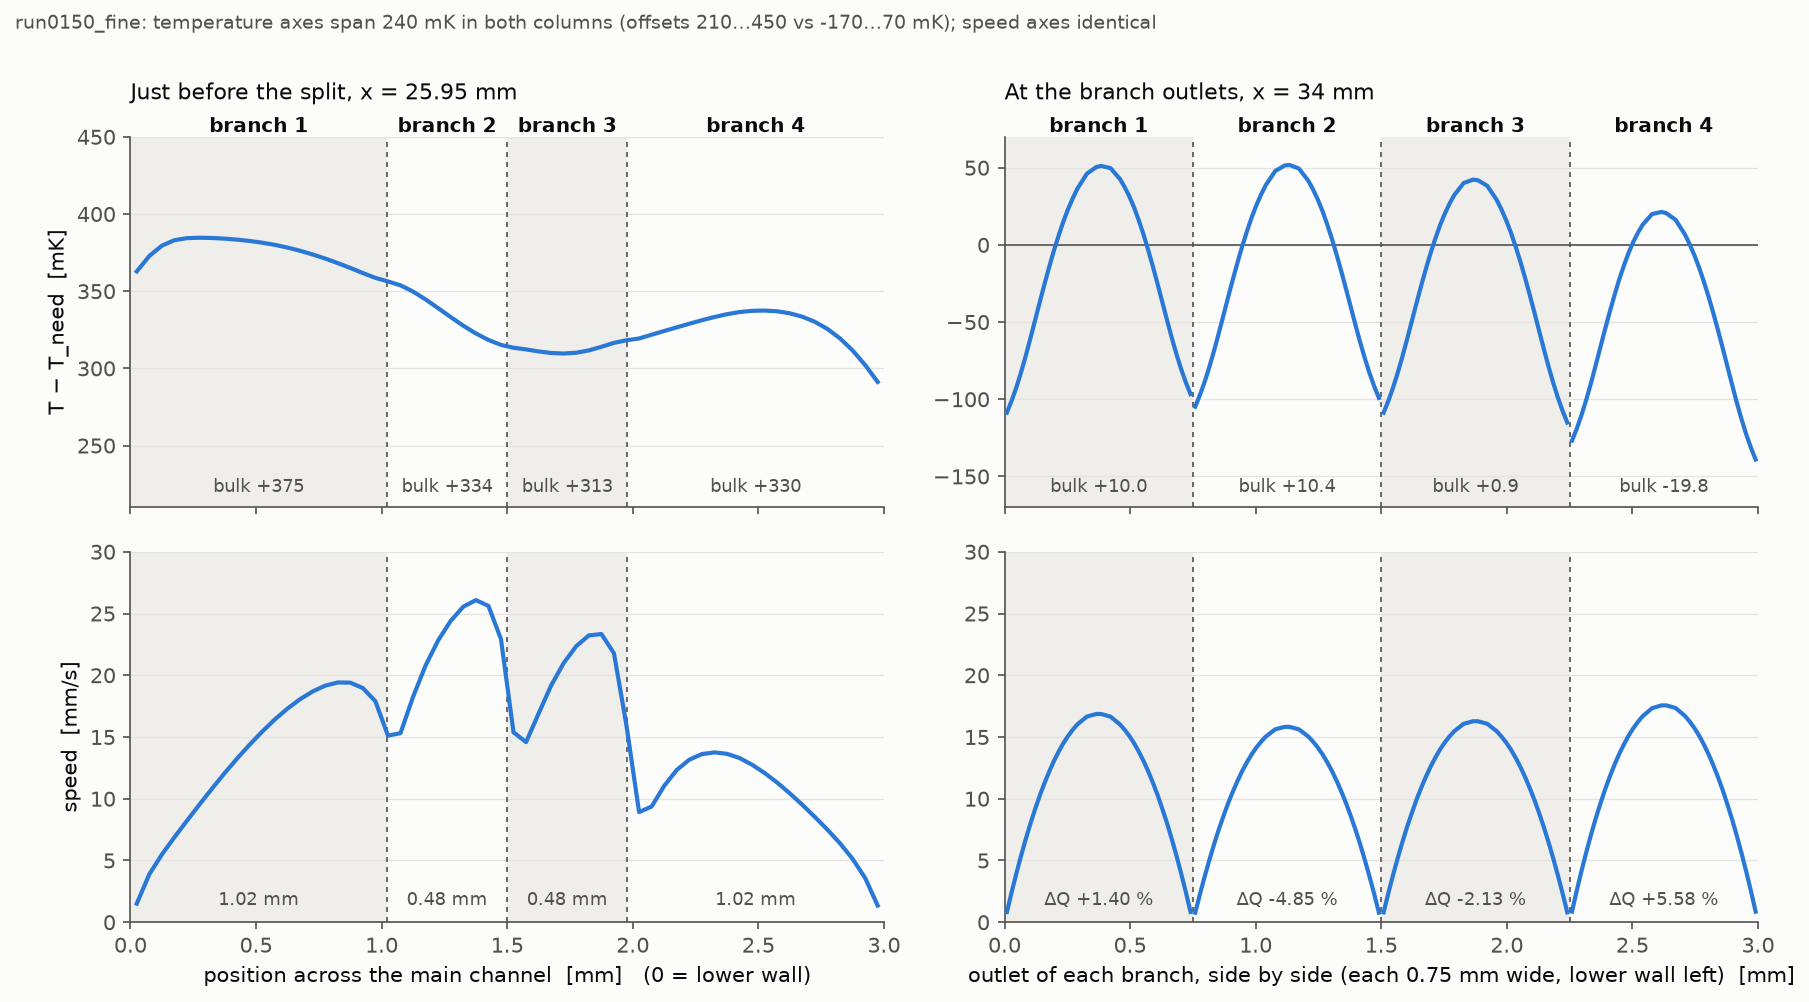
\includegraphics[width=0.95\textwidth,height=0.8\textheight,keepaspectratio]{runs/final_b2d_serp_presplit.png}
\caption{Cross-section just before the split, cut into the four branch inlets, next to each branch outlet.}
\end{figure}
\begin{figure}[H]\centering
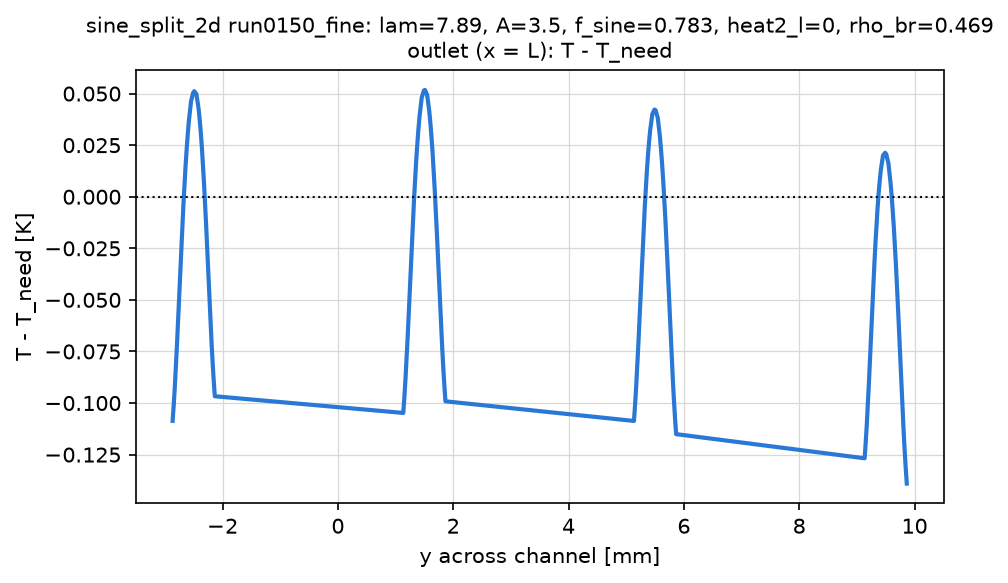
\includegraphics[width=0.75\textwidth,height=0.8\textheight,keepaspectratio]{runs/final_b2d_serp_outlet.png}
\caption{Outlet temperature (and, in 3D, the outlet plane).}
\end{figure}
\begin{figure}[H]\centering
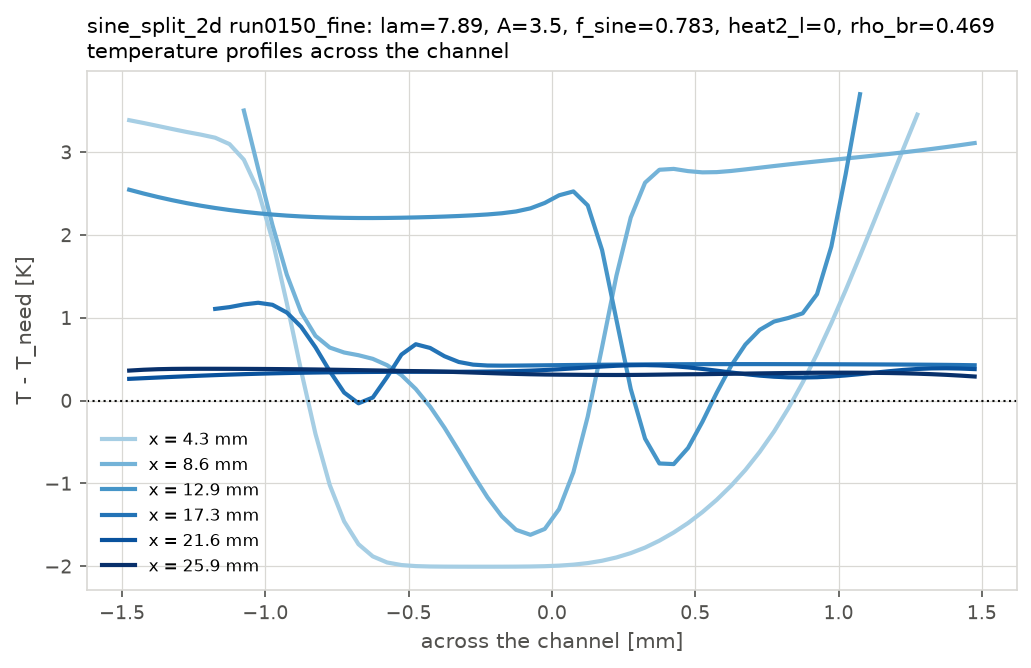
\includegraphics[width=0.62\textwidth,height=0.8\textheight,keepaspectratio]{runs/final_b2d_serp_slices.png}
\caption{Temperature profiles across the channel at several $x$ stations.}
\end{figure}
\begin{figure}[H]\centering
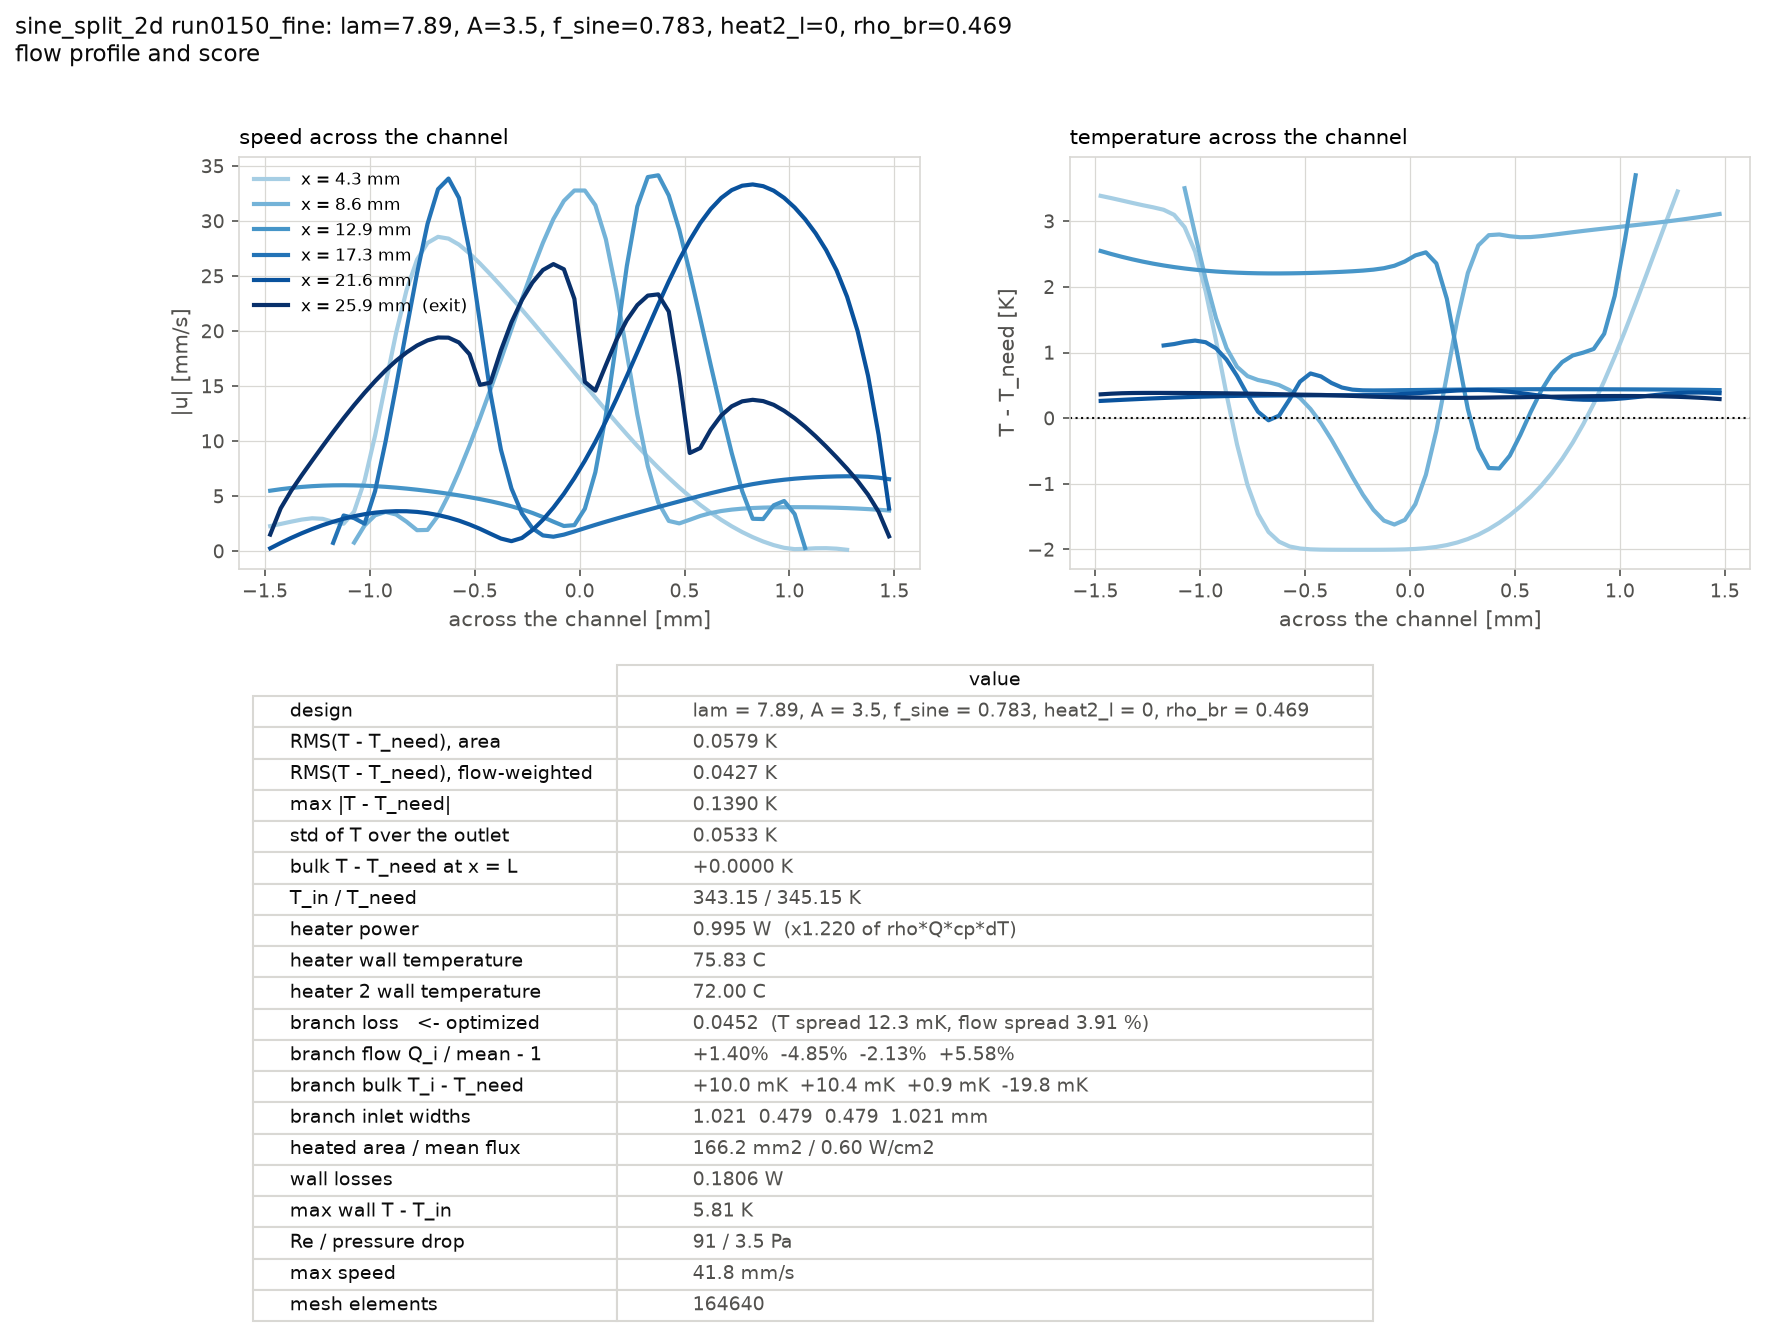
\includegraphics[width=0.8\textwidth,height=0.8\textheight,keepaspectratio]{runs/final_b2d_serp_profile.png}
\caption{Speed and temperature across the channel at several $x$ stations, and the full score table of the design.}
\end{figure}
\begin{figure}[H]\centering
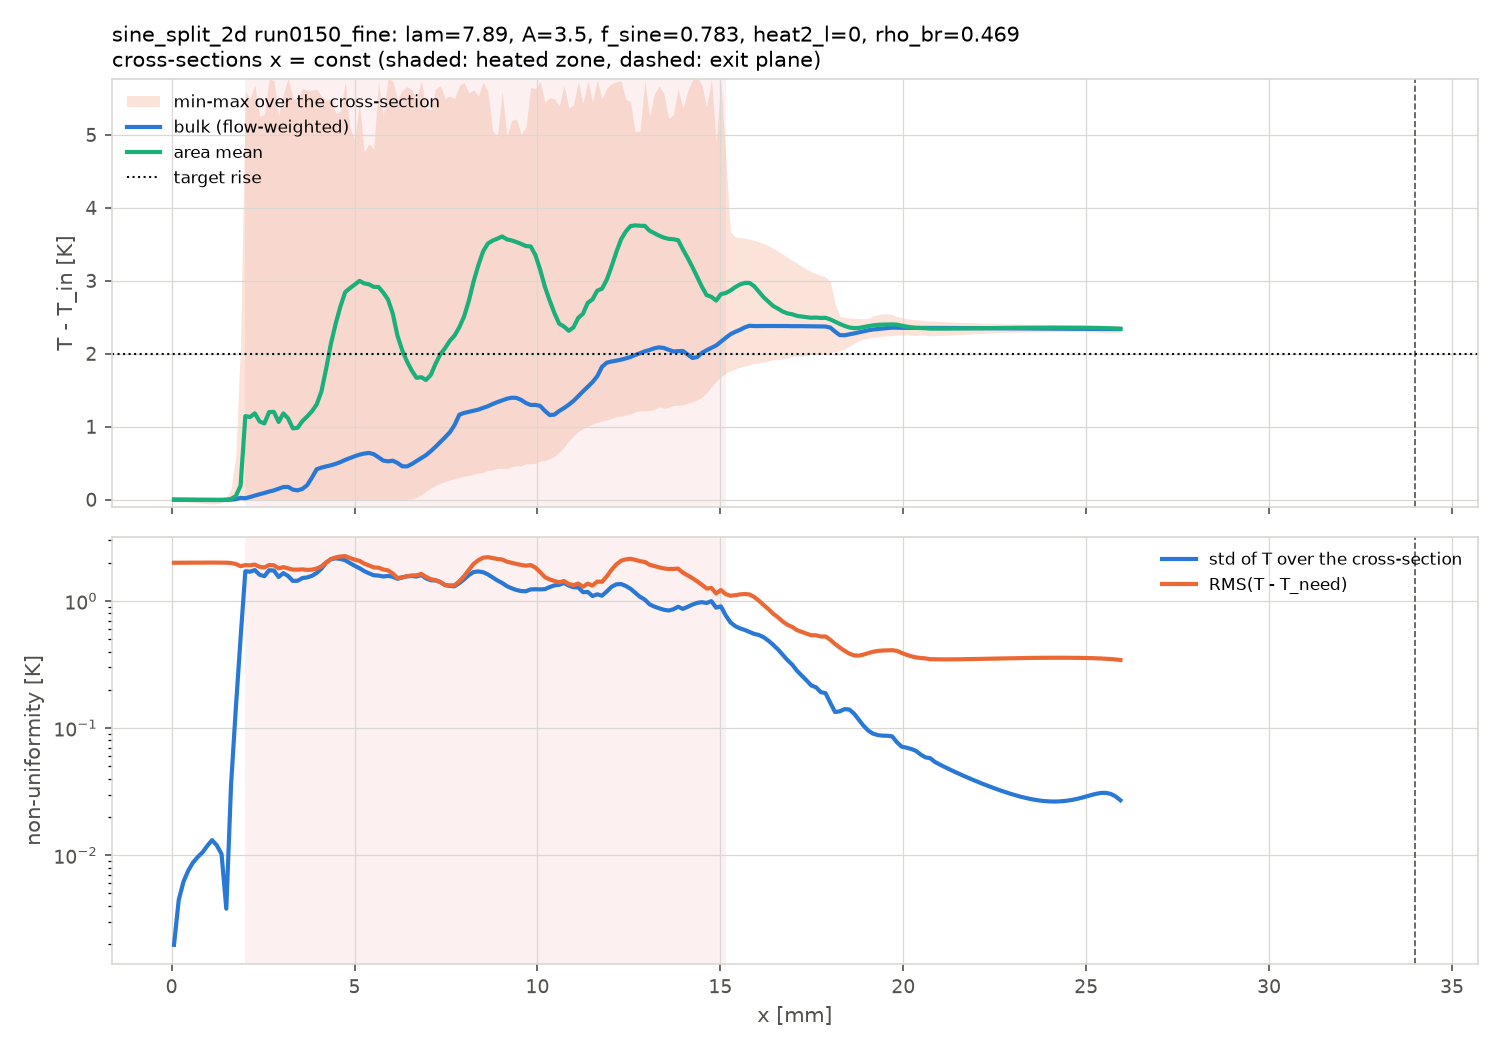
\includegraphics[width=0.8\textwidth,height=0.8\textheight,keepaspectratio]{runs/final_b2d_serp_along_x.png}
\caption{Bulk, mean, min and max temperature along the channel.}
\end{figure}
\begin{figure}[H]\centering
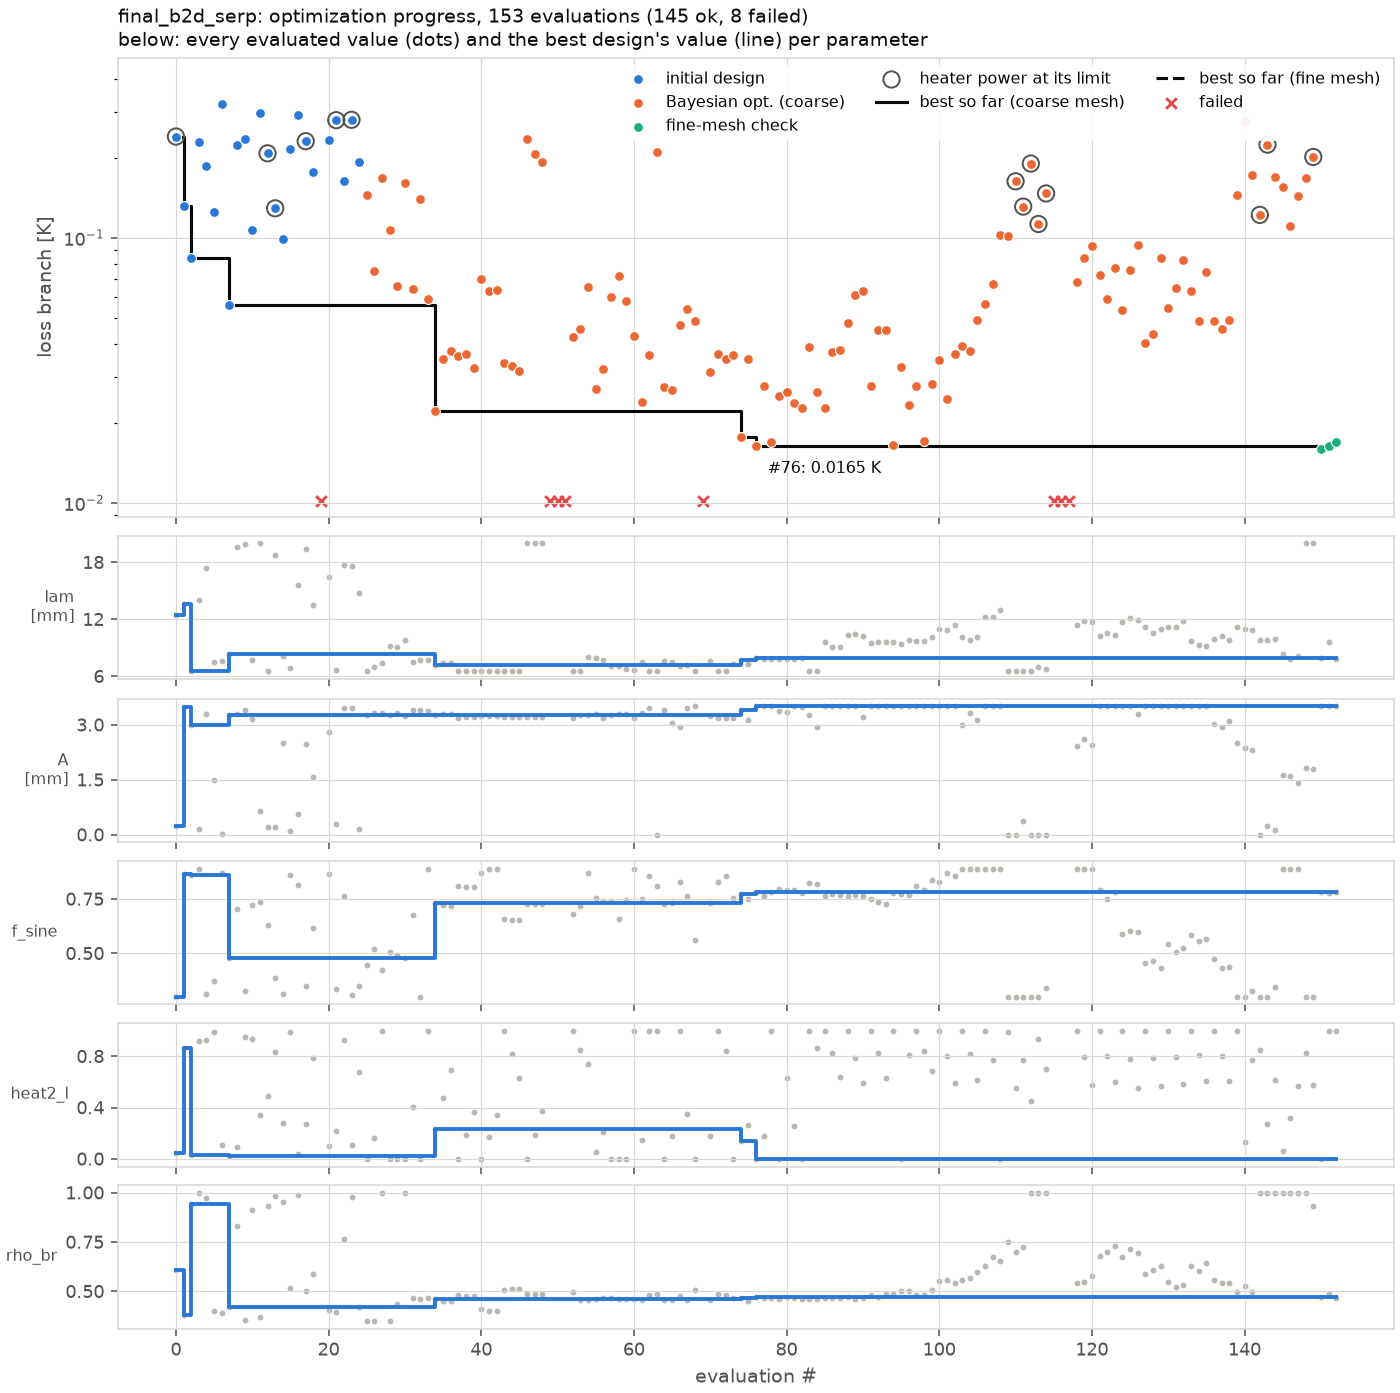
\includegraphics[width=0.85\textwidth]{runs/final_b2d_serp_progress_loss.png}
\caption{Search history: loss of every evaluation, best so far, and the parameters.}
\end{figure}


\end{document}
